\documentclass[12pt, twoside, bahasa]{report}
\title{Buku Tesis}

% Jika pakai windows untuk run pertama kali dan error.
% Mohon cek miktex console jika compiler latex nya menggunakan miktex.

\usepackage[indonesian]{babel}
\usepackage[pdfauthor={Nur Rohman Widiyanto},bookmarksnumbered,pdfborder={0 0 0}]{hyperref}
\usepackage[ruled,lined,commentsnumbered,linesnumbered]{algorithm2e}
\usepackage[utf8]{inputenc}
\usepackage{graphicx}
\usepackage{rotating}
\usepackage{booktabs}
\usepackage[ruled,lined,commentsnumbered,linesnumbered]{algorithm2e}
\usepackage{algpseudocode}
\usepackage{makeidx}
\makeindex
\usepackage{epsfig}
\usepackage{subfig}
\usepackage{pdflscape}
\usepackage[doublespacing]{setspace}
\setstretch{1.5}
\usepackage{type1cm}
\usepackage{lettrine}
\usepackage{hyperref}
\usepackage[pageref]{backref}
\usepackage{multirow}
\usepackage[table,xcdraw]{xcolor}
\usepackage{fancyhdr}
\usepackage{etoolbox}
\usepackage{url}
\usepackage{longtable}
\usepackage{float}
\usepackage{morefloats}
\floatstyle{boxed}
\newfloat{program}{thp}{lop}
\floatname{program}{Program}
\usepackage{amsmath}
\usepackage{amsfonts}
\usepackage{amssymb}
\usepackage{nccmath}
\usepackage{enumitem}
\usepackage{nonfloat}
\usepackage{ulem}
\usepackage[final]{pdfpages}
\usepackage{titlesec}
\usepackage{array}
\usepackage{multicol}
\usepackage{listings}
\usepackage{wrapfig}
\usepackage{array,tabularx}
\usepackage{lscape}
\usepackage{longtable}
\usepackage{caption}
\usepackage[export]{adjustbox}
\usepackage{ragged2e}
\usepackage{epsfig}
\usepackage{subfig}
\usepackage[top=35mm,left=40mm,right=30mm,bottom=30mm]{geometry}
\usepackage{pdflscape}
\usepackage[doublespacing]{setspace}
\setstretch{1.5}
\usepackage{type1cm}
\usepackage{lettrine}
\usepackage[pageref]{backref}
\usepackage{multirow}
\usepackage[table,xcdraw]{xcolor}
\usepackage{fancyhdr}
\usepackage{etoolbox}
\usepackage{url}
\usepackage{longtable}
\usepackage{float}
\usepackage{morefloats}
\floatstyle{boxed}
\newfloat{program}{thp}{lop}
\floatname{program}{Program}
\usepackage{enumitem}
\usepackage{nonfloat}
\usepackage{ulem}
\usepackage{titlesec}
\usepackage{array}
\usepackage{multicol}
\usepackage{listings}
\usepackage{wrapfig}
\usepackage{array,tabularx}
\usepackage{lscape}
\usepackage{longtable}
\usepackage{natbib}
\usepackage[export]{adjustbox}
\usepackage{ragged2e}
\usepackage[utf8]{inputenc}
\usepackage{afterpage}
\usepackage{nameref}

% Background untuk pengesahan
\usepackage{eso-pic}
\newcommand\BackgroundImage{
	\put(0,0){
		\parbox[b][\paperheight]{\paperwidth}{
			\vfill
			\centering
			
\includegraphics[height=\paperheight,
			keepaspectratio]{lainnya/img/pengesahan_edit.jpg}
			\vfill
		}
	}
}

% Sub sub section indent
\usepackage{changepage}
\newenvironment{subs}
{\adjustwidth{2em}{0pt}}
{\endadjustwidth}


% Set paper size and margin
\usepackage{geometry}
\geometry{
	a4paper,
	left=40mm,
	top=35mm,
	right=30mm,
	bottom=30mm,
}

% Line spacing
\linespread{1.5}

% fix titlesec bug
\makeatletter
\patchcmd{\ttlh@hang}{\parindent\z@}{\parindent\z@\leavevmode}{}{}
\patchcmd{\ttlh@hang}{\noindent}{}{}{}
\makeatother

% Pengaturan format Chapter dan Section
\titleformat{\chapter}[display]{\bfseries\Large}{BAB \centering\thechapter}{0ex}{\vspace{0ex}\centering}[\vspace{3ex}]
\titlespacing*{\chapter}{0pt}{-4ex}{0pt}
\titleformat{\section}{\bfseries\large}{\MakeUppercase{\thesection}}{1ex}{}
\titlespacing{\section}{0pt}{0pt}{1ex}
\titlespacing{\subsection}{0pt}{0pt}{1ex}
\titlespacing{\subsubsection}{0pt}{0pt}{1ex} 

% Keterangan rumus
\newenvironment{conditions}
{\par\vspace{\abovedisplayskip}\noindent
	\tabularx{\columnwidth}{>{$}l<{$} @{${}={}$} >{\raggedright\arraybackslash}X}}
{\endtabularx\par\vspace{\belowdisplayskip}}

% Caption label bold
\usepackage[labelfont=bf]{caption}
\captionsetup{labelfont=bf}

% Jarak caption dengan obyek
\captionsetup[figure]{font=small,skip=15pt}
\captionsetup[table]{font=small,skip=15pt}

% Caption nama
\renewcommand{\figurename}{Gambar}
\renewcommand{\tablename}{Tabel}
\renewcommand{\lstlistingname}{Kode}

% Cek nomor halaman
\usepackage{changepage}

% Cek spelling
\usepackage{lipsum}
\hyphenation{meng-gerak-kan mem-per-kenal-kan pe-ri-la-ku di-je-las-kan mem-bu-tuh-kan me-ne-rap-kan hu-jan di-nya-ta-kan va-ria-bel nor-vig per-hi-tung-an chal-leng-ing al-go-rit-ma deng-an dung-eon me-nye-le-sai-kan gen-re ber-gen-re peng-gu-na-an-nya ol-ah-ra-ga ber-da-sar-kan di-ku-ra-ngi mem-bang-un be-ru-pa}

% Definisi untuk "Hati ini sengaja dikosongkan"
\def\kosong{
	\vspace*{\fill}
	\begin{center}\textit{Halaman ini sengaja dikosongkan}\end{center}
	\vfill
}

% Untuk citation
\newcommand{\tab}[1]{\hspace{.2\textwidth}\rlap{#1}}
\renewcommand*{\backreflastsep}{, }
\renewcommand*{\backreftwosep}{, }
\renewcommand*{\backref}[1]{}
\renewcommand*{\backrefalt}[4]{
	\ifcase #1
	No citations.
	\or
	(Dikutip pada halaman #2).
	\else
	(Dikutip pada halaman #2).
	\fi
}

% Pengaturan penomoran halaman menggunakan package fancyhdr
\fancyhf{} 								% Mengosongkan header dan footer
\renewcommand{\headrulewidth}{0pt} 		% Menghapus garis horizontal pada header
\pagestyle{fancy} 						% Mengubah pagestyle dokumen menjadi fancy
\fancyfoot[CE,CO]{\thepage}				% Footer kanan pada hal. ganjil dan sebaliknya
\patchcmd{\chapter}{plain}{fancy}{}{} 	% Mengubah pagestyle pada chapter menjadi fancy
\patchcmd{\chapter}{empty}{plain}{}{}

% Dokumen setiap bab
\begin{document}
\singlespacing

% Cover Warna
\thispagestyle{empty}
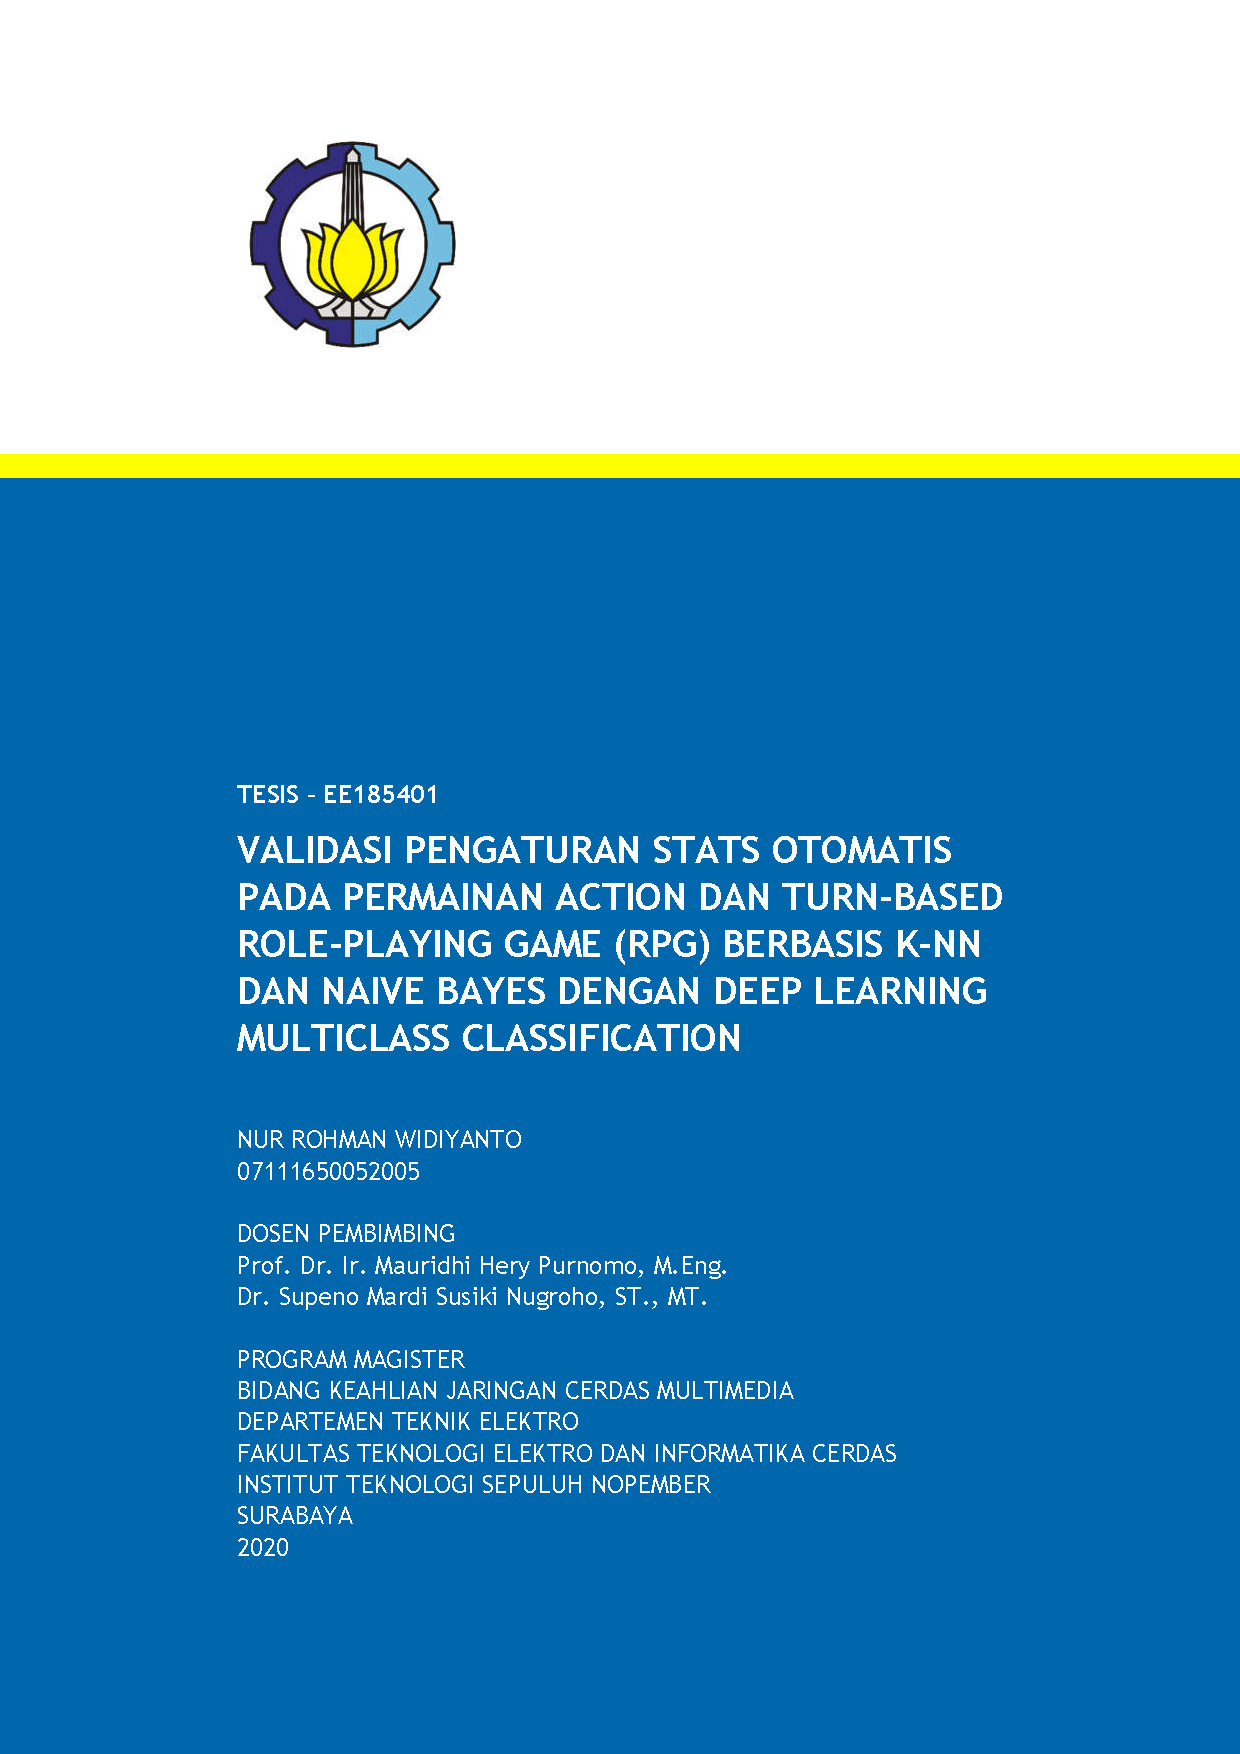
\includepdf[pages={1-2}]{cover/cover_word.pdf}
\newpage

% Halaman dimulai dari sini
\pagenumbering{roman}

% Cover BW
\thispagestyle{empty}
\includepdf[pages={3-4}]{cover/cover_word.pdf}
\newpage

% Tambahkan kata "Hati ini sengaja dikosongkan" pada \cleardoublepage 
\patchcmd{\cleardoublepage}{\hbox{}}{\kosong}{}{}

% Lembar Pengesahan
\addcontentsline{toc}{chapter}{LEMBAR PENGESAHAN}
\AddToShipoutPicture*{\BackgroundImage}

\begin{center}
	\Large\textbf{LEMBAR PENGESAHAN TESIS}
\end{center}

\begin{center}
	Tesis disusun untuk memenuhi salah satu syarat memperoleh gelar\\
	\textbf{Magister Teknik (MT)}\\
	di\\
	\textbf{Institut Teknologi Sepuluh Nopember}\\
	Oleh:\\
	\textbf{NUR ROHMAN WIDIYANTO}\\
	\textbf{NRP: 07111650050205}
\end{center}

\begin{center}
	Tanggal Ujian: 17 Juni 2020\\
	Periode Wisuda: September 2020
\end{center}

\begin{table}[!h]
\centering
\vspace{-8ex}
\caption*{}
\label*{}
\begin{tabular}{lll}
	\multicolumn{3}{c}{Disetujui oleh:} \\
	\multicolumn{3}{c}{\textbf{Pembimbing:}} \\
	&  &  \\
	1 & Prof. Dr. Ir. Mauridhi Hery Purnomo, M.Eng & ................................... \\
	& NIP: 195809161986011001 &  \\
	&  &  \\
	&  &  \\
	2. & Dr. Supeno Mardi Susiki Nugroho, ST., MT & ................................... \\
	& NIP: 197003131995121001 &  \\
	&  &  \\
	\multicolumn{3}{c}{\textbf{Penguji:}} \\
	&  &  \\
	1. & Dr. Eko Mulyanto Yuniarno, ST., MT. & ................................... \\
	& NIP: 196806011995121009 &  \\
	&  &  \\
	&  &  \\
	2. & Dr. Diah Puspito Wulandari, ST. M.Sc & ................................... \\
	& NIP: 198012192005012001 &  \\
	&  &  \\
	&  &  \\
	3. & Reza Fuad Rachmadi, ST., MT., Ph.D & ................................... \\
	& NIP: 198504032012121001 &  \\
	&  &  \\
	&  &  \\
	\multicolumn{3}{c}{Kepala Departemen Teknik Elektro} \\
	\multicolumn{3}{c}{Fakultas Teknologi Elektro} \\
	&  &  \\
	&  &  \\
	&  &  \\
	&  &  \\
	\multicolumn{3}{c}{\underline{Dedet Candra Riawan, ST., M.Eng, Ph.D.}} \\
	\multicolumn{3}{c}{NIP: 197311192000031001}
\end{tabular}
\end{table}

\newpage
\cleardoublepage

% Pernyataan Keaslian
\addcontentsline{toc}{chapter}{PERNYATAAN KEASLIAN}
\begin{center}
\large\textbf{PERNYATAAN KEASLIAN TESIS}
\end{center}
\vspace{1ex}
\begin{spacing}{1.5}

\setlength{\parindent}{0.9cm} Dengan ini saya menyatakan bahwa isi buku Tesis dengan judul ``\textbf{PERHITUNGAN KENAIKAN ATRIBUT \textit{GAMEPLAY} UNTUK PEMAIN DAN \textit{NON-PLAYER CHARACTER} PADA PERMAINAN \textit{ROLE-PLAYING GAME} BERBASIS K-NN DAN NAIVE BAYES}'' adalah benar hasil karya intelektual mandiri, diselesaikan tanpa menggunakan bahan-bahan yang tidak diijinkan dan bukan merupakan karya pihak lain yang saya akui sebagai karya sendiri.
\vspace{1ex}

Semua referensi yang dikutip maupun dirujuk telah ditulis secara lengkap pada daftar pustaka. Apabila ternyata pernyataan ini tidak benar, saya bersedia menerima sanksi sesuai peraturan yang berlaku.
\vspace{1ex}
\end{spacing}
\begin{flushright}
\begin{tabular}[b]{c}
  Surabaya, Agustus 2020\\
  \\
  \\
  \\
  \\
  Nur Rohman Widiyanto\\
  07111650050205
\end{tabular}
\end{flushright}
\cleardoublepage

% Abstrak Indonesia
\addcontentsline{toc}{chapter}{ABSTRAK}
\begin{spacing}{1}
	\begin{center}
		\large\textbf{PERHITUNGAN KENAIKAN ATRIBUT \textit{GAMEPLAY} UNTUK PEMAIN DAN \textit{NON-PLAYER CHARACTER} PADA PERMAINAN \textit{ROLE-PLAYING GAME} BERBASIS K-NN DAN NAIVE BAYES}
	\end{center}
	\vspace{2ex}
	
	\begin{adjustwidth}{-0.2cm}{}
		\begin{tabular}{lcp{0.7\linewidth}}
			Nama Mahasiswa &:& Nur Rohman Widiyanto \\
			NRP &:&	07111650050205 \\
			Pembimbing &:& 1. Prof. Dr. Ir. Mauridhi Hery Purnomo, M.Eng. \\
			& & 2. Dr. Supeno Mardi Susiki Nugroho, ST., MT. \\
		\end{tabular}
	\end{adjustwidth}
	\vspace{2ex}
	
	\begin{center}
		\large\textbf{ABSTRAK}
	\end{center}
	\vspace{1ex}
	
	Permainan dengan genre \textit{Role Playing Game} (RPG) merupakan permainan yang bersifat kompetitif, antara pemain melawan pemain ataupun melawan musuh yang berupa \textit{Non-Player Character} (NPC). Banyak pengembang permainan dalam pembuatan permainan itu sendiri masih menggunakan cara manual dalam penentuan atribut \textit{gameplay} untuk karakter pemain ataupun musuh. Terlebih lagi, saat sebuah permainan memiliki banyak karakter, seperti hanyalnya banyak karakter pemain (contohnya pada JRPG dan TRPG) dan juga banyak musuh. Pada penelitian ini diimplementasikan beberapa pendekatan seperti halnya $k-$NN, Distribusi Normal, dan Naive Bayes yang akan digunakan dalam program penghitung kenaikan atribut \textit{gameplay} pada karakter pemain dan musuh secara otomatis. Pada program tersebut dibutuhkan parameter masukan yang akan menentukan atribut \textit{gameplay} yang akan dihasilkan. Untuk karakter pemain, dibuatlah skenario atribut \textit{gameplay} berdasarkan peran setiap karakter yang ingin dibuat seperti \textit{knight}, \textit{priest}, \textit{assassin}, dan lain-lain. Sedangkan pada karakter musuh, dalam distribusi atribut \textit{gameplay} juga dibagi menjadi beberapa tipe musuh yang dicontohkan seperti \textit{mixed}, \textit{hard strength}, \textit{hard magic}, dan lain-lain. Setelah itu, hasil atribut \textit{gameplay} diklasifikasi dengan menggunakan \textit{Neural Network Multiclass Classification}. Hal tersebut bertujuan untuk menghitung tingkat kesesuaian atribut \textit{gameplay} dari karakter pemain dan musuh yang dihasilkan. Operasi tersebut dilakukan secara terpisah pada atribut \textit{gameplay} pemain dan musuh, karena tidak adanya hubungan saat pembuatan atau perhitungan. Masing-masing dibagi kedalam data \textit{training} dan \textit{testing}, dengan perbandingan 70\% dan 30\%. Proses tersebut menghasilkan keluaran berupa tipe karakter pemain dan musuh pada data \textit{testing}, hal tersebut diperoleh dari proses \textit{training}. Presentase kesesuaian tersebut diperoleh dengan membandingkan tipe pada karakter yang diperoleh dari hasil klasifikasi pada data \textit{testing} dengan tipe dari karakter yang sebenarnya, maka diperolehlah sebuah presentase banyaknya karakter yang berhasil terklasifikasi.
	\vspace{2ex}
	
	% Kata Kunci : Kecerdasan buatan, \textit{Reinforcement Learning}, \textit{Non-Playable Character}, \textit{Turn-based}, RPG (\textit{Role Playing Game}).

	Kata Kunci: \textit{Role-Playing Game}, Atribut \textit{Gameplay}, $k-$NN, Naive Bayes, \textit{Neural Network}, Klasifikasi.
\end{spacing}
\cleardoublepage

% Abstrak Inggris
\addcontentsline{toc}{chapter}{ABSTRACT}
\begin{spacing}{1}
	\begin{center}
		\large\textbf{VALIDATING THE AUTOMATIC STATS ADJUSTMENT IN ROLE-PLAYING GAME (RPG) BASED ON K-NN AND NAIVE BAYES WITH NEURAL NETWORK MULTICLASS CLASSIFICATION}
	\end{center}
	\vspace{2ex}
	
	\begin{adjustwidth}{-0.2cm}{}
		\begin{tabular}{lcp{0.7\linewidth}}
			By &:& Nur Rohman Widiyanto \\
			Student Identity Number &:&	07111650050205 \\
			Supervisors &:& 1. Prof. Dr. Ir. Mauridhi Hery. P, M.Eng. \\
			& & 2. Dr. Supeno Mardi Susiki. N, ST., MT. \\
		\end{tabular}
	\end{adjustwidth}
	\vspace{2ex}
	
	\begin{center}
		\large\textbf{ABSTRACT}
	\end{center}
	\vspace{1ex}
	
	The game with the Role Playing Game (RPG) genre was a competitive game, between players against other players or against enemies with form of Non-Player Character (NPC). Many game developers when makes the game itself still uses manual approach when determine the statistical data for the player or enemy character. When in a game has a lot of characters, such as only a lot of player characters (for example on JRPG and TRPG) and many enemies. In this research several approaches such as $k-$NN (Nearest Neighbor) was implemented, Normal Distribution and Naive Bayes which used to generate statistical data for player characters and enemy automatically. Then, the Neural Network Multiclass Classification will be used for validate the stats that was generated before.
	\vspace{2ex}

	Keywords: Role-Playing Game (RPG), Stats, $k-$NN, Naive Bayes, Neural Network, Classification.
\end{spacing}
\cleardoublepage

% Kata pengantar
\addcontentsline{toc}{chapter}{KATA PENGANTAR}
\begin{center}
\Large\textbf{KATA PENGANTAR}
\end{center}
\vspace{2ex}

\setlength{\parindent}{1cm} Puji dan syukur kehadirat Allah SWT atas segala limpahan berkah, rahmat, serta hidayah-Nya, penulis  dapat menyelesaikan penelitian ini dengan judul \textbf{Validasi Pengaturan \textit{Stats} Otomatis pada Permainan \textit{Role-Playing Games} (RPG) Berbasis K-NN dan Naive Bayes dengan \textit{Neural Network Multiclass Classification}}.
\vspace{1ex}

Penelitian ini disusun dalam rangka pemenuhan bidang riset di Jurusan Teknik Elektro ITS, Bidang  Studi Teknik Komputer dan Telematika, serta digunakan sebagai persyaratan menyelesaikan pendidikan  S1. Penelitian ini dapat terselesaikan tidak lepas dari bantuan berbagai pihak. Oleh karena itu, penulis mengucapkan terima kasih kepada:
\vspace{1ex}

\begin{enumerate}[nolistsep]
	\item Keluarga, Ibu, Bapak dan Saudara tercinta yang telah memberikan dorongan spiritual dan material dalam penyelesaian penelitian ini.
	\vspace{1ex}
	\item Bapak Dr. Tri Arief Sardjono, ST., MT. selaku Dekan Fakultas Teknologi Elektro ITS, Bapak Ronny Mardiyanto, ST., MT., Ph.D. selaku Ketua Program Pasca Sarjana FTE Teknik Elektro ITS, Serta Bapak Eko Mulyanto, S.T., M.T. Selaku Ketua Program bidang keahlian Jaringan Cerdas Multimedia FTE Teknik Elektro ITS.
	\vspace{1ex}
	\item Secara khusus penulis mengucapkan terima kasih yang sebesar-besarnya kepada Bapak Prof. Dr. Ir. Mauridhi Hery Purnomo, M.Eng. dan Bapak Dr. Supeno Mardi Susiki Nugroho, ST., MT. atas bimbingan selama mengerjakan  penelitian.
	\vspace{1ex}
	\item Bapak-ibu dosen pengajar Bidang Keahlian Jaringan Cerdas Multimedia, atas pengajaran,  bimbingan, serta perhatian yang diberikan kepada penulis selama ini.
	\vspace{1ex}
	\item Seluruh teman-teman \textit{B201-crew} Laboratorium Bidang Studi Teknik Komputer dan Telematika.
\end{enumerate}
\vspace{1ex}

Kesempurnaan hanya milik Allah SWT, untuk itu penulis memohon segenap kritik dan saran yang  membangun. Semoga penelitian ini dapat memberikan manfaat bagi kita semua. Amin.
\vspace{26pt}

\begin{flushright}
	\begin{tabular}[b]{c}
		Surabaya, Juni 2020
		\\
		\\
		\\
		\\
		Penulis
	\end{tabular}
\end{flushright}
\cleardoublepage

% Daftar isi
\renewcommand*\contentsname{DAFTAR ISI}
\titlespacing*{\chapter}{0pt}{0ex}{0ex}
\tableofcontents
\cleardoublepage

% Daftar gambar
\renewcommand*\listfigurename{DAFTAR GAMBAR}
\addcontentsline{toc}{chapter}{\listfigurename}
\titlespacing*{\chapter}{0pt}{0ex}{0ex}
\listoffigures
\cleardoublepage

% Daftar tabel
\renewcommand*\listtablename{DAFTAR TABEL}
\addcontentsline{toc}{chapter}{\listtablename}
\titlespacing*{\chapter}{0pt}{0ex}{0ex}
\listoftables
\cleardoublepage

% Nomenklatur
\addcontentsline{toc}{chapter}{NOMENKLATUR}
\begin{center}
\large\textbf{NOMENKLATUR}
\end{center}
\vspace{1ex}
\begin{conditions}
	x &	Data x atau titik koordinat data.\\
	x_{0} & Titik koordinat data ke 0.\\
	x_{i} &	Data $x$ ke $i$.\\
	x_{n} & Data $x$ ke $n$.\\
	\theta & Data $\theta$.\\
	\theta_{i} & Data $\theta$ ke $i$.\\
	min\ d & Jarak minimum\\
	i & Urutan atau iterasi.\\
	Y & Titik Y.\\
	y & Bagian dari Y dengan banyak data.\\
	X & Titik X.\\
	D & Distance atau jarak.\\
	p & Data p atau titik koordinat data.\\
	p_{i} & Titik koordinat data ke $i$.\\
	y_{pred} & Hasil prediksi dari titik koordinat yang dicari.\\
	y_{i} & Titik koordinat yang dicari oleh $y_{pred}$.\\
	k & Nilai $k$ dalam $k$-NN.\\
	P(h|d) & Probabilitas hipotesis $h$ berdasrkan data $d$. Hal ini disebut probabilitas posterior.\\
	P(d|h) & Probabilitas dari data $d$ berdasarkan hipotesis $h$ yang bernilai benar.\\
	P(h) & Probabilitas hipotesis $h$ yang bernilai benar terlepas dari data secara keseluruhan.\\
	P(d) & Probabilitas data secara keseluruhan terlepas dari hipotesis.\\
	MAP(h) & Maximum a Posteriori Probability.\\
	P(C) & \textit{Class pobability}.\\
	C & \textit{Class} untuk dicari probabilitasnya.\\
	W & \textit{Weather} atau cuaca pada contoh kasus Naive Bayes.\\
	n & Jumlah data.\\
	\bar{x} & Rata-rata nilai $x$.\\
	\sigma(x) & Standar deviasi.\\
	PDF & Probability Density Function.\\
	B_{total} & Jumlah waktu melawan bos secara keseluruhan.\\
	HP & Health Point.\\
	MP & Magic Point.\\
	MaxSt & Jarak maksimum stats.\\
	St_{i} & Stats ke $i$.\
\end{conditions}
\newpage
\cleardoublepage

% Bab isi buku
\titleformat{\chapter}[display]{\bfseries\Large}{BAB \centering\thechapter}{0ex}{\vspace{0ex}\centering}[\vspace{0ex}]
\titleformat{\section}{\bfseries\large}{\MakeUppercase{\thesection}}{1ex}{}
\titleformat{\subsection}{\bfseries\large}{\MakeUppercase{\thesubsection}}{1ex}{}
\titleformat{\subsubsection}{\bfseries\large}{\MakeUppercase{\thesubsubsection}}{1ex}{}
\titlespacing*{\chapter}{0pt}{-4ex}{0pt}
\titlespacing{\section}{0pt}{0pt}{0pt}
\titlespacing{\subsection}{0pt}{0pt}{0pt}
\titlespacing{\subsubsection}{0pt}{0pt}{0pt}

% Indent paragraph
\setlength{\parindent}{1cm}
\begin{spacing}{1.5}
	\chapter{PENDAHULUAN}
\pagenumbering{arabic}
\vspace{4ex}
\label{chap:chap1_introduction}

\section{Latar Belakang}
\vspace{1ex}

Permainan dengan basis \textit{Role-Playing Game} (RPG) adalah permainan yang mana pemain memerankan sebuah karakter khusus dalam sebuah cerita. Pada permainan tersebut, pemain memiliki tujuan untuk menjalankan misi dan mengikuti alur cerita dari permainan tersebut sampai selesai. Terdapat berbagai macam variasi jenis dari RPG, salah satunya adalah \textit{turn-based}. Pada \textit{turn-based} RPG, pemain dapat memainkan satu karakter atau lebih yang mana karakter tersebut melakukan serangan secara bergantian antara pemain atau musuh seperti pada Gambar \ref{fig:rpg_turn_based}. Biasanya musuh yang dilawan berupa \textit{Non-Player Character} (NPC).
\vspace{1ex}

\begin{figure} [!h] \centering
	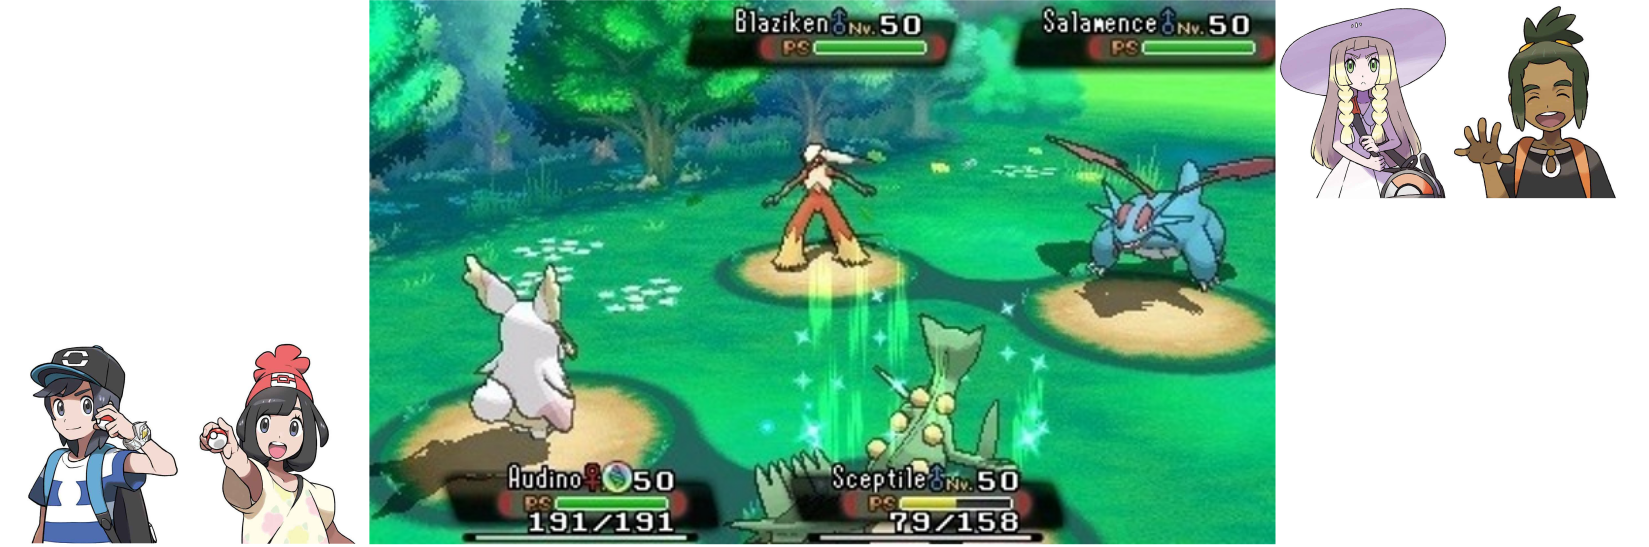
\includegraphics[scale=0.40]{img/turn_based.png}
	\caption{Ilustrasi \textit{Turned-based} RPG}
	\label{fig:rpg_turn_based}
\end{figure}

Pada permainan dengan genre \textit{turn-based} RPG yang terdiri dari banyak karakter baik itu karakter pemain dan musuh. Di mana stats tersebutlah yang akan menentukan jalannya pertarungan antara pemain dan musuh. Kemudian stats juga menunjukan tingkat kesulitan dari musuh, kelemahan dari musuh, daya tahan musuh terhadap serangan dan lain-lain. Hal ini juga merupakan bagian utama dari desain permainan, yang mana nominal pada stats, jumlah pemain dan musuh dapat menentukan beberapa faktor penting lain seperti halnya lamanya permainan dan alur cerita. 
\vspace{1ex}

Banyak penelitian yang mengaplikasikan berbagai bentuk algoritma dan metode untuk mempercepat pembuatan \textit{video games} sepeti halnya pengukuran tingkat kesulitan dengan menggunakan challenging rate (CR) pada permainan 2D \textit{Real Time Strategy} (RTS) \citep{Christyowidiasmoro2016}, pembuatan \textit{game engine} yang berorientasi pada \textit{multi-agent systems} \citep{Marin-Lora2020}, pembuatan level secara otomatis pada permainan secara prosedular dengan tingkat kesulitan tertentu \citep{Wu2018}, ada juga ada yang memakai metode yang dapat menghasilkan \textit{attribute space} untuk menganalisa keseimbangan dalam pertarungan \textit{single unit} pada permainan RTS \citep{Bangay2014}. Berdasarkan beberapa penelitian tersebutlah maka penelitian ini dibuat guna memudahkan desainer permainan dalam mendesain sebuah permainan dengan genre \textit{action} dan \textit{turn-based} RPG.
\vspace{1ex}

Penggunaan berbagai metode seperti $k-$NN, Distribusi Normal dan Naive bayes yang kemudian dilanjutkan dengan diperolehnya data statistik dari untuk pemain dan musuh yang siap digunakan. Kemudian dilanjutkan dengan proses validasi data statistik tersebut apakah sudah sesuai dengan apa yang direncanakan. Pada proses tersebut digunakanlah \textit{Deep Learning} dengan basis \textit{Neural Network} untuk \textit{Multiclass Classification}.
\vspace{1ex}

\section{Rumusan Masalah}
\vspace{1ex}

Pembuatan statistik untuk karakter yang akan dimainkan oleh pemain dan juga karakter musuh pada permainan dengan genre action dan turn-based RPG yang terkadang masih dilakukan secara manual, terlebih lagi jika karakter dari pemain dan musuh pada permainan tersebut sangat banyak maka diperlukannya sebuah program yang mampu menyusun hal tersebut secara otomatis.
\vspace{1ex}

\section{Tujuan}
\vspace{1ex}

Dari permasalahan yang dirumuskan sebelumnya,maka penelitian ini memiliki tujuan sebagai berikut: 

\begin{enumerate}
	\item Mempercepat proses desain permainan dengan menggunakan program yang dapat menghasilkan data statistik untuk karakter dari pemain dan musuh.

	\item Terujinya data statistik untuk karakter pemain dan musuh yang dihasilkan secara otomatis oleh program.
\end{enumerate}

\section{Batasan Masalah}
\vspace{1ex}

Berdasrkan fokus permasalahan pada bagian sebelumnyaa, kemudian diambilah beberapa pembatasa masalah. Berikut adalah batasan-batasan masalah tersebut.

\begin{enumerate}
	\item Data statistik yang dihasilkan oleh program hanya dapat dipakai oleh permainan dengan genre \textit{action} dan \textit{turn-based} RPG.
	
	\item Program yang dibuat untuk menghasilkan data statistik dapat dipakai oleh lebih sama dengan satu karakter pemain dan musuh.

	\item Metode yang digunakan dalam proses pembuatan data statistik pemain dan musuh diantaranya adalah $k-$NN, Normal Distribution dan Naive Bayes.
	
	\item Sedangkan metode yang digunakan untuk menguji tingkat ke validitas dari data yang dibuat tadi digunakanlah metode \textit{deep learning} berbasis \textit{Neural Network} dengan \textit{Multiclass Classification}.
\end{enumerate}

\section{Kontribusi}
\vspace{1ex}

Di harapkan penelitian ini mampu mejadi rujukan dalam proses desain permainan, khususnya saat pembuatan data statistik untuk karakter pemain dan musuh. Selain itu menjadikan para pengembang permainan dengan genre RPG khususnya \textit{action} dan \textit{turn-based} RPG di masa mendatang menjadi lebih cepat.

	\cleardoublepage
	\chapter{KAJIAN PUSTAKA}
\label{chap:chap2_kajian_pustaka}

\section*{}
Demi mendukung penelitian ini, dibutuhkan beberapa teori penunjang sebagai bahan acuan dan referensi. Berikut adalah paparan teori dasar meliputi komponen desain permainan, \textit{machine learning}, dan penjelasan permainan genre RPG (\textit{Role-Playing Game}).
\vspace{1ex}

\section{Kajian penelitian terkait}
\label{sec:sec2_kajian}
\vspace{1ex}

Beberapa penelitan sebelumnya yang berkaitan dengan penelitian ini dan mendukung penelitian ini antara lain:

\begin{enumerate}
	\item Paper dengan judul ``\textit{Measuring Level of Difficulty in Game Using Challenging Rate (CR) on 2D Real Time Strategy Line Defense Game}'' yang ditulis oleh Christyowidiasmoro dan rekan-rekan tahun 2015. Meneliti tentang formula \textit{Challenging Rate} (CR) adalah formula yang menggunakan elemen dasar dalam permainan RTS (\textit{Real Time Strategy}) sebagai parameternya. Dalam tulisan ini dibuat sebuah \textit{prototipe} permainan dengan tingkat kesulitan yang diajukan untuk mencoba kemampuan formula \textit{Challenging Rate} untuk mengukur nilai tingkat kesulitan.

	\item Paper dengan judul ``\textit{A game engine to make games as multi-agent systems}'' yang ditulis oleh Carlos Marín-Lora dan rekan-rekan tahun 2019. Pada tulisan ini meneliti tentang pengembangan \textit{game engine} yang berfokus pada multi-agen. Di mana pada setiap aktor atau agen-agen memiliki sejumlah properti dan aturan kebiasaan untuk berinteraksi dengan lingkungan dalam permainan. Tujuan dari engine tersebut adalah memenuhi kebutuhan dasar dari sistem multi agent dengan merubah karakteristik dari system tanpa adanya pengaruh terhadap potensi karakter.

	\item Paper dengan judul ``\textit{Procedurally Generating Game Level with Specified Difficulty}'' yang ditulis oleh Zong-Han Wu dan rekan-rekan tahun 2018. Penelitian ini mencakup ranah pembuatan konten dalam sebuah permainan secara prosedural, hal tersebut bertujuan agar para pemain memperoleh pengalaman yang berbeda dalam bermmain. Pada paper ini yang paling banyak di ulas adalah permainan PAC-MAN, dengan labirin yang dapat berubah secara procedural.
	
	\item Paper dengan judul ``\textit{Generating an Attribute Space for analyzing Balance in Single Unit RTS Game Combat}'' yang ditulis oleh Shaun Bangay dan Owen Makin tahun 2014. Fokus pada tulisan ini adalah tentang pencapaian keseimbangan dalam permainan \textit{Real Time Strategy} (RTS), dengan dibuatnya sebuah \textit{framework} yang dinamakan dengan \textit{attribute space}. Pendekatan ini dievaluasi dan direpresentasikan untuk pertarungan \textit{single unit} atau satu lawan satu pada permainan RTS. Melalui proses tersebut kemudian dibuatlah model prediksi terhadap simulasi pertarungan tersebut, dengan menggunakan attribut atau data statistik pada permainan tersebut seperti halnya \textit{speed}, \textit{range}, \textit{health} dan \textit{damage}.
\end{enumerate}

\section{Desain Permainan RPG dan Komponennya}
\label{sec:sec2_gdd}
\vspace{1ex}

Desain permainan adalah proses menciptakan konten dan aturan permainan. Desain permainan yang baik adalah proses menciptakan tujuan agar seorang pemain merasa termotivasi untuk mencapainya dan aturan yang dibuat dapat diikuti oleh seorang pemain saat membuat keputusan untuk mengejar tujuan-tujuan tersebut \citep{Brathwaite2009}. Berikut adalah sebagian elemen dari desain permainan yang akan digunakan pada permainan dengan genre RPG pada penelitian ini.
\vspace{1ex}

\subsection{Penempatan Peluang pada Permainan}
\label{sec:sub_sec2_kesempatan}
\vspace{1ex}

Sebagian besar permainan setidaknya mengandung beberapa faktor acak. Misalnya, banyak permainan kartu melibatkan proses acak. Adanya variabel \textit{damage} dipertarungan pada sebagian besar permainan dengan genre RPG. Permainan seperti \textit{Rock-Paper-Scissors} memiliki pola yang tampak acak, meskipun terlihat tanpa mekanisme acak. Pada bagian ini akan banyak membahas mengenai aspek acak pada permainan dan bagaimana \textit{developer} akan menggunakannya.
\vspace{1ex}

Pada dasarnya permainan yang memasukan unsur keberuntungan dapat dimainkan dan dimenangkan oleh khalayak luas. Bila dicari alasan penggunaannya, hasilnya sangatlah banyak. Pada akhirnya harus diakui bahwa hal-hal tersebut adalah keputusan dari desainer permaninan untuk menciptakan dinamika yang dikehendakinya. Berikut adalah contoh-contoh penerapan penempatan peluang pada permainan yang biasanya diterapkan.
\vspace{1ex}

\begin{enumerate}[label=\textbf{\alph*).}]

	\item \textbf{Menunda atau Mencegah Penyelesaian Masalah}
	\setlength{\parindent}{0.8cm}

	Untuk permainan yang memiliki sedikit cara penyelesaian saat dipecahkan oleh komputer dan terutama manusia. Maka sesuatu harus dilakukan untuk menjaga permainan agar tetap \textit{fresh} dan menyenangkan. Di tambahkanlah elemen acak untuk mencapai tujuan tersebut. Hal tersebut bertujuan agak pemain tidak terlalu menguasai permainan, karena saat pemain membuat keputusan yang sama persis dapat memberi hasil yang berbeda. Hal tersebut tentunya juga berpengaruh pada tingkat rasa bosan pemain dalam memainkan sebuah permainan, jika pola yang sama terus muncul.
	\vspace{1ex}

	\item \textbf{Membuat Permainan Lebih Kompetitif}

	Elemen acak yang sesekali memungkinkan pemain yang kurang berpengalaman untuk menang atau setidaknya menawarkan keuntungan yang membuat permainan ini bertahan lebih lama dengan menggunakan dua cara. Pertama adalah selalu ada peluang kemenangan bagi setiap pemain. Kemudian yang kedua adalah efek dari kekalahan berkurang ketika seorang pemain bisa menyalahkan nasib buruknya sendiri atas kekalahannya. Hal tersebut tentunya juga dapat memunculkan rasa tidak terima akan sebuah kekalahan dan dimulainya permainan baru lagi.
	\vspace{1ex}
	
	\item \textbf{Meningkatkan Keberagaman}

	Permainan tanpa elemen acak selalu dimulai dengan cara yang sama dan pola-pola tertentu seperti langkah awal pada permainan Catur. Akibatnya, pemain dapat memiliki pengalaman yang sama dari satu pertandingan ke pertandingan yang lain, dan para pemain dapat mejatuhkan pilihannya untuk selalu memakai strategi yang sama.
	\vspace{1ex}

	\item \textbf{Menciptakan Momen Dramatis}

	Ketika seorang pemain dengan hati-hati menyusun strategi dan kemudian harus bergantung pada lemparan dadu atau apa pun yang bersifat acak untuk melihat apakah rencana tersebut berhasil, momen tersebut bisa menjadi sangat menegangkan. \textit{Role-Playing Games} (RPG), \textit{Real-Time Strategy} (RTS) dan banyak \textit{board game} yang mengandalkan kondisi ini saat bermain. Akankah \textit{healing spell} (mantra penyembuhan) yang digunakan akan sampai ke rekan bermainmu yang terluka sebelum monster menyerang? Apakah AI akan memberi pemain dua monster untuk bertempur ataukah hanya satu?
	\vspace{1ex}

	\item \textbf{Meningkatkan Pengambilan Keputusan}

	Inti dari sebagian besar permainan adalah keputusan yang dibuat para pemain. Dalam permainan strategi, pemain memiliki informasi lengkap dan tahu hasil pasti dari setiap gerakan yang mereka lakukan. Karena semua variabel diketahui, beberapa keputusan menjadi tidak terlalu menarik, jika ada kesempatan untuk membunuh ratu lawan pada permainan catur secara cuma-cuma tanpa ada yang perlu dikorbankan, hal tersebut bukan merupakan keputusan yang menarik karena adanya jawaban ``benar" yang jelas. Ketika elemen acak ada dalam permainan, tidak ada lagi strategi yang selalu benar. Beberapa gerakan mungkin memiliki peluang kegagalan yang tinggi tetapi juga potensi hasil yang besar, hal tersebut menjadikannya sebuah pilihan berisiko, gerakan lainnya mungkin aman tetapi menghasilkan sedikit keuntungan. Hal tersebut menjadikan pemain akan melakukan analisis gerakan dengan cara yang berbeda berikut risiko dan keutungan yang akan didapat, kemudian tidak lupa mempertimbangkan posisi pemain tersebut dalam permainan atau langkah selanjutnya.
	\vspace{1ex}
	
\end{enumerate}

\subsection{Elemen Keterampilan Strategi}
\label{sec:sub_sec2_strategi}
\vspace{1ex}

Strategi adalah salah satu kekuatan yang dapat dilakukan oleh para pemain. Karena hal tersebutlah yang membuat para pemain tetap bermain. Pemain bermain \textit{game} dan menikmati setiap prosesnya karena mereka berusaha untuk menguasai pola dalamnya \citep{Koster2013}. Saat pola berhasil dikuasai, maka selanjutnya pemain akan terus bersenang-senang. Mereka juga membentuk strategi berdasarkan pemahaman mereka tentang dinamika permainan. Penguasaan, pengembangan strategi, hal tersebut terjadi bukan karena ketidak sengajaan. 
\vspace{1ex}

Hal ini adalah tujuan dari desainer permainan atas penggunaan mekanika untuk menciptakan strategi dan taktik dalam permainan yang mereka buat \cite{Brathwaite2009}. Berikut beberapa poin penting pada penelitian ini yang mengacu tentang pentingnya Elemen Keterampilan Strategi.
\vspace{1ex}

\begin{enumerate}[label=\textbf{\alph*).}]
	
	\item \textbf{Peran dari Keterampilan pada Permainan}
	\setlength{\parindent}{0.8cm}

	Permainan yang bagus dibangun dari serangkaian keputusan menarik, membangun unit untuk menyerang atau bertahan, mencari tahu apa yang harus dilakukan oleh unit tersebut selanjutnya, apa saja kelemahannya dan lain sebagainya. Keberhasilan keputusan tersebut juga didasari oleh reaksi dari mental atau fisik pemain, karena hal tersebut adalah ukuran keterampilan dari seorang pemain.
	\vspace{1ex}

	Permainan yang bagus menyebabkan pemain sering melatih kemampuannya dan memberi \textit{reward} atau bonus dengan pola timbal balik yang jelas. Kemudian sepanjang permainan pemain bertanya-tanya tentang apa yang harus dilakukan selanjutnya. Masuklah mereka ke dalam istilah yang disebut dengan ``lingkaran sihir" sebuah \textit{video game}, melalui monitor atau TV sebagai medianya terseraplah mereke ke dalam dunia game. Efek tersebut sama seperti ketika menonton film atau membaca buku yang sangat menarik, tetapi permainan yang baik memiliki daya tarik yang lebih kuat karena terjadi interaksi antara pemain dan keputusan yang dibuat yang terkonversi menjadi sebuah pengalaman.
	\vspace{1ex}
	
	Ketika pemain terus-menerus membuat keputusan, secara tidak sadar mereka telah memasuki kondisi yang oleh psikolog dan peneliti terkenal Mihaly Csikszentmihalyi disebut ``\textit{flow}". Hal tersebut adalah keadaan permainan yang optimal dan merupakan hasil kerja keras dari seorang desainer pemainan. Csikszentmihalyi menulis seluruh buku tentang topik, \textit{Flow: The Psychology of Optimal Experience}. Buku ini tidak terbatas pada permainan saja, tetapi mencakup keadaan semacam ini dari perspektif yang lebih luas.
	\vspace{1ex}
	
	\item \textbf{Strategi dan Taktik}
	
	Secara teknis strategi utama adalah keseluruhan cara untuk mencapai tujuan akhir jangka panjang (misalnya, kemenangan dalam permainan). Strategi utama terdiri dari beberapa strategi pendukung dengan tujuan jangka pendek atau menengah yang harus dilakukan untuk mencapai strategi besar (misalkan dalam peperangan besar, pilihan untuk bertarung dalam pertempuran tertentu adalah sebuah pilihan strategis). Taktik adalah keputusan mikro tingkat terendah yang dibuat ketika menjalankan strategi misalkan pada pergerakan pasukan, apakah akan diperintahkan untuk melakukan serangan udara, kapan pasukan haarus mulai bergerak, dimana posis yang tepat untuk menempatkannya, kapan mulai menembak dan lain-lain adalah contoh keputusan taktis yang dibuat selama pertempuran militer. Secara informal pemain dalam permainan membuat keputusan strategis ketika membuat rencana jangka panjang (panjangnya strategi tersebut bersifat relatif terhadap panjangnya permainan), dan keputusan taktis ketika pemain ingin mencapai tujuan jangka pendek.
	\vspace{1ex}
	
	Pengorbanan mejadikan pengambilan keputusan atau pembuatan taktik menjadi lebih menarik. Keputusan yang diambil secara cepat atau \textit{twitch mechanics}, bisa disebut juga dengan ketangkasan memiliki keterbatasan pada taktik. Hal ini menunjukkan bahwa permainan yang lebih fokus pada strategi, umumnya bersifat giliran atau \textit{turn-based} seperti Catur dan \textit{Go}, yang mana lebih terfokus pada keputusan yang melibatkan pengorbanan.
	\vspace{1ex}
	
	\item \textbf{Game Berbasis Keterampilan Sepenuhnya}
	
	Permainan yang fokus pada strategi dan pengorbanan cenderung memiliki setidaknya beberapa elemen peluang. Ketika permainan-permainan ini murni berbasis keterampilan, seperti \textit{Tic-Tac-Toe} atau sebagian besar \textit{video game} petualangan, mereka dapat diselesaikan, dan keputusan-keputusan yang tadinya bervariasi kemudian menjadi keputusan-keputusan yang jelas. Misalkan dalam membuat keputusan pada akhirnya hanya ada satu gerakan atau pilihan benar.
	\vspace{1ex}
	
	Sebagian besar game yang sepenuhnya berupa keterampilan adalah game aksi berbasis fisik. Mungkin hal inilah sebabnya, tidak seperti pada pengorbanan yang bukan tentang mendapatkan jawaban yang benar atau terbaik melainkan mendapatkannya dengan cepat. Waktu reaksi atau tindakan manusia dapat terus meningkat dari waktu ke waktu selamanya, terutama pada permainan dimana manusia saling berlawanan satu dengan yang lain atau \textit{multiplayer}.
	\vspace{1ex}
\end{enumerate}

\subsection{Menemukan Keseimbangan}
\label{sec:sub_sec2_keseimbangan}
\vspace{1ex}

Beberapa permainan sangat terlihat jelas bahwa semua membutuhkan keterampilan. Hal ini sangat bervariasi dari yang sederhana (\textit{Tic-Tac-Toe}) menuju yang lebih kompleks (Catur dan \textit{Go}). Ada juga perbedaan antara keterampilan berbasis strategis (seperti pada kebanyakan permainan berbasis strategi dan giliran) dan kemampuan pengambilan keputusan secara cepat atau \textit{twitch} (biasa ditemukan dalam permainan berbasis keterampilan dan olahraga) atau bisa disebut juga dengan ketangkasan. Permainan ini bisa menjadi sangat menyenangkan karena terdapat keputusan berarti yang dibuat oleh pemain, baik itu keputusan yang dibuat dengan cepat (\textit{twitch}) dan keputusan yang dibuat berdasarkan strategi \citep{Brathwaite2009}.
\vspace{1ex}

Banyak permaian yang menggabungkan kedua basis di atas. \textit{Settlers of Catan} memiliki banyak elemen \textit{gameplay} berbasis keterampilan, termasuk perdagangan, pembangunan, dan manajemen sumber daya. Namun permainan tersebut juga memiliki dadu, setumpuk kartu yang dikocok secara acak, dan pengaturan papan yang disusun dengan acak. \textit{Backgammon} dan \textit{Poker} keduanya memiliki elemen keterampilan dan keberuntungan yang kuat. Bayangkan sebuah permainan \textit{Backgammon} tanpa dadu, atau \textit{Poker} tanpa kemampuan untuk bertaruh atau menggertak lawan, dan menjadi jelas bahwa beberapa permainan mampu menjadi lebih baik dengan adanya campuran keterampilan dan peluang. Jika salah satunya dihapus maka permainan tersebut tidak akan menjadi menarik.
\vspace{1ex}

Bagaimana seorang desainer permainan memasukkan campuran keterampilan dan peluang yang benar dalam sebuah permaian? Kapan saat yang tepat untuk mengarahkan permainan ke arah itu? Jawabannya adalah kembali kepada siapakah pemainnya?
\vspace{1ex}

Hal tersebut adalah pertanyaan penting, seringkali pertanyaan pertama yang diajukan seorang desainer. Ketika merancang permainan untuk anak berusia enam tahun hasil yang diperoleh akan sangat berbeda jika dibandingkan dengan merancang permainan yang diperuntukkan bagi mahasiswa. Pemain yang berbeda memiliki tingkat toleransi yang berbeda untuk setiap peluang dan keterampilannya. Permainan yang mungkin menjadi sangat populer bagi para gadis muda bisa jadi menjadi membosankan bagi orang dewasa, karena sebagai orang tua yang telah memainkan sejumlah permainan anak-anak dan dapat mengujinya. Beberapa contoh target pemain seperti anak-anak, pemain permainan kompetitif, permainan sosial, pemain profesional dan keluarga. Dalam penelitian ini akan difokuskan dengan permainan kompetitif, karena fokus utamanya adalah \textit{fun games}.
\vspace{1ex}

Pemain permainan kompetitif cenderung lebih menyukai permainan dengan lebih banyak elemen keterampilan. Hal ini memberi mereka kesempatan untuk bermain satu lawan satu dengan pemain lain, mencocokan setiap pemikiran menjadi sebuah strategi, refleks melawan refleks, strategi melawan strategi. Hal terakhir yang diinginkan oleh pemain yang benar-benar kompetitif adalah proses acak seperti halnya dengan penggelindingan dadu yang merusak permainan yang dieksekusi dengan sempurna dan terampil.
\vspace{1ex}

Mengapa desainer menambah keberuntungan pada permainan berbasis keterampilan? Banyak alasan yang membuat hal-hal tidak dapat diprediksi, meningkatkan kemampuan pemain dengan memainkan permainan itu lagi, dan memungkinkan pemain dengan keterampilan yang sedikit berbeda untuk tetap dapat bersaing. Jika pemain yang lebih baik selalu menang, maka satu-satunya pertarungan yang menarik adalah antara dua pemain dengan kemampaun yang sama rata.
\vspace{1ex}

\section{Machine Learning}
\label{sec:sec2_ML}
\vspace{1ex}

\textit{Machine Learning} (ML) adalah studi ilmiah tentang algoritma dan model statistik yang digunakan oleh komputer untuk melakukan tugas tertentu secara efektif tanpa menggunakan instruksi secara eksplisit, dengan mengandalkan pola dan inferensi sebagai gantinya. \textit{Machine learning} juga dilihat sebagai bagian dari kecerdasan buatan. Algoritma dari \textit{machine learning} membangun model matematika berdasarkan data sampel, yang dikenal sebagai ``data training'' dalam membuat prediksi atau keputusan tanpa diprogram secara eksplisit untuk melakukan tugasnya \citep{Koza1996}. Kemudian setelah dilakukannya \textit{training} maka dapat digunakan untuk menyelesaikan permasalahan dari tujuan dibutnya \textit{machine learning} itu sendiri, atau yang biasa disebut dengan proses \textit{testing}.
\vspace{1ex}

Algoritma \textit{machine learning} dapat digunakan pada berbagai aplikasi, seperti penyaringan email, dan visi komputer, yang mana tidak mungkin untuk mengembangkan algoritma instruksi khusus untuk melakukan tugas dengan sendirinya. \textit{Machine learning} terkait erat dengan komputasi statistik yang berfokus pada pembuatan prediksi dengan menggunakan komputer. Studi tentang optimasi matematika memberikan metode, teori dan domain aplikasi ke bidang \textit{machine learning}. Penambangan data atau \textit{data mining} adalah bidang studi yang termasuk ke dalam cakupan \textit{machine learning}, dan berfokus pada analisis dan eksplorasi data melalui pembelajaran yang mampu berjalan secara otomatis \citep{Friedman1997}.
\vspace{1ex}

Pada penelitian ini akan digunakan beberapa algoritma \textit{machine learning} untuk menyelesaikan permasalahan dalam mendesain permainan. Penggunaan algoritma tersebut secara umum adalah membuat data baru yang terstruktur dengan referensi data awal yang disesuaikan dengan kebutuhan untuk mendesain permaian. Berikut algoritma-algoritma tersebut dan penjelasannya secara umum nantinya, di mana natinya akan dipakai dan dijelaskan secara detail pada BAB \ref{chap:chap3_metodologi}.
\vspace{1ex}

\subsection{K-Nearest Neighbor}
\label{sec:sub_sec2_knn}
\vspace{1ex}

Di asumsikan terdapat sampel $(x_{i}, \theta_{i})$ yang didistribusikan secara sesuai dengan distribusi $(x, \theta)$ argumen heuristik tertentu yang memungkinkan dalam prosedur pengambilan keputusan. Contohnya saat pengasumsian tentang jarak dari beberapa data, metrik atau koordinat yang sesuai akan diklasifikasi berdasarkan kesamaannya atau setidaknya memiliki kesamaan distribusi pada setiap datanya. Maka dalam klasifikasi sampel $x$, dipertimbangkan berdasarkan $x_{i}$ terdekat yang diasumsikan sebagai kemungkinan terbesar. Sehingga prosedur pengambilan keputusan paling sederhana adalah aturan \textit{nearest neighbor} (NN) dengan mengklasifikasikan $x$ sebagai tetangga terdekat.
\vspace{1ex}

Di buatlah satu set $n$ pasangan $(x_{1}, \theta_{2}), ..., (x_{n}, \theta_{n})$, yang mana $x_{i}$'s mengambil nilai dalam metrik $X$ yang didefinisikan sebagai metrik $d$, dan $O_{i}$ nilai yang diambil di set $\{1, 2, ..., M\}$ seperti pada persamaan \ref{eq: KNN_all_x_data} dan \ref{eq: KNN_distance}. Setiap $\theta_{i}$ dianggap sebagai indeks dari kategori yang dimiliki oleh data ke-$i$, dan setiap $x_{i}$ adalah hasil dari pengukuran setiap data. Lebih singkatnya pada ``$x_{i}$ bagian dari $\theta_{i}"$ adalah saat data ke-$i$ yang menjadi dasar pengukuran $x_{i}$ yang telah diamati dan diukur, termasuk juga pada kategori $\theta_{i}$.
\vspace{1ex}

Di lakukan beberapa penambahan pasangan baru $(x,$ $\theta)$, yang mana pengukuran $x$ yang akan dilakukan, dan digunakan hasilnya digunakan untuk memperkirakan $\theta$ dengan memanfaatkan hasil pengukuran atau klasifikasi sebelumnya. Pada persamaan \ref{eq: KNN_all_x_data} dinyatakan bahwa seluruh data $x$ atau $x_{n}$ yang akan diguanakan untuk mecari nilai $\theta$.

\begin{equation}\label{eq: KNN_all_x_data}
x'_{n}\ \epsilon\ x_{1}, x_{2},\ ...,\ x_{n}
\end{equation}

\noindent Akan termasuk ke dalam \textit{nearest neighbor} terhadap $x$ jika dilanjutkan dengan persammaan berikut.

\begin{equation}\label{eq: KNN_distance}
min\ d(x_{i}, x) = d(x'_{n}, x),\ \ \ i = 1, 2,\ ...,\ n
\end{equation}

Aturan \textit{nearest neighbor} menentukan, apakah $x$ termasuk dalam kategori $\theta'_{n}$ dari tetangga terdekatnya $x'_{n}$ seperti pada persamaan \ref{eq: KNN_distance} di mana metrik $d$ adalah \textit{distance} atau jarak. Kesalahan dibuat jika $\theta'_{n} \neq \theta$. Perhatikan bahwa aturan \textit{nearest neighbor} hanya menggunakan klasifikasi berdasarkan tetangga terdekat saja. Sedangkan $n - 1$ yang merupakan sisa hasil klasifikasi $\theta_{i}$ akan diabaikan \citep{Cover1967}. Dengan demikian, metode klasifikasi berbasis $k-$NN dapat dengan mudah diterapkan dalam banyak tugas klasifikasi. Secara umum, sebagian besar varian $k-$NN menentukan label kelas dari sampel data dengan menggunakan satu parameter $k$ yang merupakan jarak dari keseluruhan data yang di anggap sebagai \textit{neighbour} dan juga keputusan di ambil dengan mempertimbangkan jarak data secara mayoritas. Tetapi keputusan klasifikasi tersebut dapat dengan mudah dipengaruhi oleh sensitivitas $k$ itu sendiri dan juga dapat memperburuk sensitivitasnya, sehingga sangat menurunkan kinerja klasifikasi dari $k-$NN terutama dalam kasus ukuran sampel yang kecil.

\begin{enumerate}[label=\textbf{\alph*).}]
	
	\item \textbf{Klasifikasi}
	\setlength{\parindent}{0.8cm}
	
	Dalam mendemonstrasikan analisis $k-$\textit{nearest neighbor}, dipertimbangkan juga proses klasifikasi objek baru (koordinat data) diantara sejumlah contoh yang diketahui. Hal ini ditunjukkan pada Gambar \ref{fig:k-nn_plus_minus}, yang menggambarkan representasi dari data atau \textit{instance} dengan tanda plus dan minus dan titik dengan lingkaran merah. Dan permasalahan yg harus diselesaikan adalah memperkirakan (klasifikasi) hasil dari titik tersebut berdasarkan sejumlah tetangga terdekat atau \textit{nearest neighbor} yang dipilih. Dengan kata lain, apakah titik tersebut dapat diklasifikasikan sebagai tanda plus atau minus.
	
	\begin{figure} [!h] \centering
		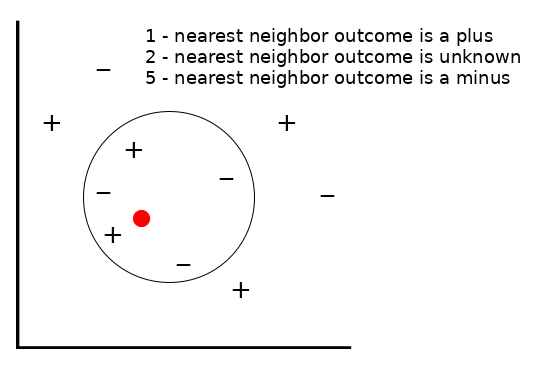
\includegraphics[scale=0.45]{img/k-nn_plus_minus.png}
		\caption{Klasifikasi dengan $k-$NN.}
		\label{fig:k-nn_plus_minus}
	\end{figure}
	
	Kemudian dipertimbangkannya hasil $k-$NN berdasarkan tetangga terdekat pertama (1-\textit{nearest neighbor}). Jelas bahwa dalam hal ini $k-$NN akan memprediksi hasil dari titik atau representsi data dengan nilai tambah (karena titik terdekat adalah tanda plus). Dilanjutkan dengan penambahan jumlah tetangga terdekat menjadi 2 (2-\textit{nearest neighbor}). Kali ini $k-$NN tidak akan dapat mengklasifikasikan hasil dari titik dari data yang dicari, karena titik terdekat keduanya adalah minus, sehingga tanda plus dan minus mencapai jarak yang sama. Untuk langkah selanjutnya, ditambahkan lagi jumlah tetangga terdekat menjadi 5 (5-\textit{nearest neighbor}). Hal ini akan menentukan daerah tetangga terdekat, yang ditunjukkan oleh lingkaran yang seperti pada Gambar \ref{fig:k-nn_plus_minus}. Karena ada 2 tanda plus dan 3 tanda minus. Pada lingkaran tersebut $k-$NN akan memberikan tanda minus pada hasil dari titik koordinat yang dicari.
	
	\item \textbf{Regresi}
	
	Pada bagian ini akan digeneralisasi konsep $k-$\textit{nearest neighbor} untuk menyelesaikan permasalahan regresi. Permasalahan regresi sangat berkaitan dengan prediksi hasil dari variabel dependen berdasarkan beberapa variabel independen. Di mulai dengan mempertimbangkan skema yang ditunjukkan pada Gambar \ref{fig:k-nn_sinosoid}, di mana satu data \textit{training} atau data sampel (kotak jingga) yang diambil dari hubungan antara variabel independen $x$ dan variabel dependen $y$ (kurva biru). 
	
	\begin{figure} [!h] \centering
		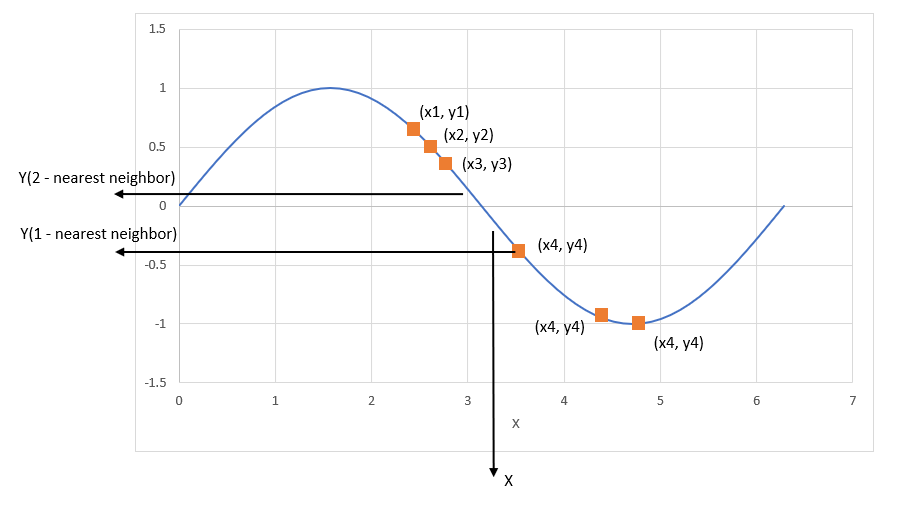
\includegraphics[scale=0.6]{img/k-nn_sinosoid.png}
		\caption{Proses regresi dengan $k-$NN.}
		\label{fig:k-nn_sinosoid}
	\end{figure}
	
	Kemudian ditandai dengan kotak jingga yang dlianjutkan dengan penerapan $k-$\textit{nearest neighbor} untuk memprediksi hasil keluaran yang ditandai dengan $X$. Kemudian direpresentasikan juga dengan kotak jingga. Di mulai dengan mempertimbangkan metode 1-\textit{nearest neighbor} sebagai data sampel. Dalam kasus ini akan dicari data sample (kotak jingga) yang paling dekat dengan titik X. Pada Gambar \ref{fig:k-nn_sinosoid} yang dicari dinyatakan dalam koordinat $(X, Y)$ sedangkan koordinat data yang paling mendekati adalah $(x_{4}, y_{4})$. Maka dapat disimpulkan bahawa tetangga terdekatnya atau \textit{nearest neighbor} adalah $(x_{4}, y_{4})$ untuk 1-\textit{nearest neighbor}.
	\vspace{1ex}
	
	Langkah selanjutnya adalah mencari 2-\textit{nearest neighbor} seperti pada Gambar \ref{fig:k-nn_sinosoid}. Pada kasus ini ditemukan dua titik terdekat dengan X atau 2-\textit{nearest neighbor}, yang kebetulan ditunjukan pada Gambar \ref{fig:k-nn_sinosoid} adalah $y3$ dan $y4$. Maka diambil rata-rata dari masing-masing nilai pada data tersebut yang dinyatkan pada persamaan \ref{eq: KNN_regresi_mean}.
	
	\begin{equation}\label{eq: KNN_regresi_mean}
	\begin{split}
	Y = \frac{y_{3} + y_{4}}{2}
	\end{split}
	\end{equation}
	
	Pada metode $k-$\textit{nearest neighbor} hasil Y dari titik X dianggap sebagai hasil rata-rata dari nilai $k-$\textit{nearest neighbor} dari tetangga terdekatnya.
	\vspace{1ex}
	
	\item \textbf{Cross-Validation}
	
	\textit{Cross-validation} adalah teknik yang dapat digunakan untuk mendapatkan estimasi model parameter yang tidak diketahui. Pembahasan ini bertujuan untuk menerapan teknik dalam memperkirakan nilai $k$. 
	\vspace{1ex}
	
	Gagasan umum dari metode ini adalah untuk membagi sampel data ke dalam sejumlah kelompok atau \textit{cluster} (diambil secara acak, \textit{sub-samples} atau bagian-bagian yang terpisah). Untuk nilai tetap pada $k$, digunakanlah $k-$NN untuk membuat prediksi pada bagian ke $v$ (mislahnya dengan penggunaan bagian $v-1$ sebagai contoh) dan kemudian digunakan untuk evaluasi kesalahan. Metode paling umum untuk analsia kesalahan pada regresi adalah dengan jumlah kuadrat atau \textit{sum of square} dan pada klasifikasi hal tersebut didefinisikan sebagai akurasi atau tingkat kebenaran klasifikasi.
	\vspace{1ex}
	
	Proses ini kemudian diterapkan secara berurutan pada semua bagian atau $v$ yang mungkin. Pada bagian terakhir, kesalahan yang dijumlahkan kemudian dirata-rata untuk menghasilkan model yang stabil (seberapa baik model memprediksi titik koordinat data). Langkah-langkah di atas kemudian diulang untuk berbagai nilai $k$ yang lain, nilai yang mencapai kesalahan terendah atau akurasi klasifikasi tertinggi dijadikan sebagai nilai optimal untuk $k$. 
	\vspace{1ex}
	
	Usaha dalam mencapai nilai optimal inilah yang kemudian disebut dengan \textit{cross-validation}. Perlu diperhatikan bahwa \textit{cross-validation} membutuhkan proses komputasi tinggi dan algoritma harus dibiarkan berjalan untuk beberapa waktu terutama saat ukuran sampel berjumlah besar. Atau nilai $k$ dapat ditentukan sendiri. Ini mungkin tindakan yang wajar jika sudah megetahui apa yang akan diambil sebagai nilai $k$, dari analisis $k-$NN sebelumnya yang mungkin dilakukan pada data yang sama atau pengamatan secara manual.
	
	\item \textbf{Jarak Metrik}
	
	Seperti disebutkan sebelumnya, pada titik data yang dicari, $k-$NN membuat prediksi berdasarkan hasil $k$ dari tetangga terdekat dengan titik itu. Oleh karena itu, untuk membuat prediksi dengan $k-$NN, sangat diperlukan pendefinisian metrik untuk mengukur jarak antara titik koordinat data dan kasus dari data sampel. 
	\vspace{1ex}
	
	Salah satu metode paling populer untuk mengukur jarak ini dikenal dengan istilah \textit{Euclidean}. Langkah-langkah lain diantaranya adalah \textit{Euclidean squared}, \textit{City-block}, dan \textit{Chebyshev} seperti yang ditunjukan pada persamaan \ref{eq:KNN_distance_metrics}.
	\vspace{1ex}
	
	\begin{equation}\label{eq:KNN_distance_metrics}
	\begin{split}
	D(x,\ p) =
	\begin{Bmatrix}
	\sqrt{(x - p)^{2}} & Eclidean\\
	(x - p)^{2} & Eclidean squared\\
	abs(x - p) & Cityblock\\
	Max(|x - p|) & Chebyshev
	\end{Bmatrix}
	\end{split}
	\end{equation}
	
	Di mana pada persamaan \ref{eq:KNN_distance_metrics} variabel $x$ dan $p$ masing-masing adalah titik koordinat data yang dicari dan data sampel. Kemudian yand dimasud dengan D adalah \textit{distance} atau jarak antara data sampel dengan koordinat data yang dicari.
	\vspace{1ex}
	
	\item \textbf{Prediksi}
	
	Setelah memilih nilai $k$, maka prediksi berdasarkan data sampel dengan menggunakan $k-$NN dapat dilakukan. Sedangkan pada regresi sepeti yang dijelaskan pada bagian sebelumnya, $k-$NN memprediksi hasil rata-rata dari $k-$\textit{nearest neighbor}.
	
	\begin{equation}\label{eq: KNN_prediction}
	\begin{split}
	y_{pred} = \frac{1}{k}\ \sum_{i = 1}^{k}\ y_{i}
	\end{split}
	\end{equation}
	
	Di mana $y_{i}$ adalah kejadian ke-$i$ pada data sampel dan $y_{pred}$ adalah hasil prediksi dari titik koordinat data yang dicari. Berbeda dengan regresi, dalam masalah klasifikasi, prediksi $k-$NN didasarkan pada skema \textit{voting} di mana pemenanglah yang akan digunakan untuk melabeli titik koordinat data yang dicari.
	\vspace{1ex}
	
	Untuk klasifikasi biasanya nilai ganjil seperti $y_{pred} = 1, 3, 5, dan$ $seterusnya$ sering digunakan untuk menghindari terjadinya \textit{ties condition}, yaitu kondisi dimana terdapat dua label kelas yang mencapai skor yang sama.
	\vspace{1ex}
	
	\item \textbf{Pembobotan Jarak}
	
	Karena prediksi $k-$NN didasarkan pada asumsi intuitif bahwa objek yang jaraknya dekat berpotensi dianggap sama. Hal tersebut sangat masuk akal dalam hal membedakan antara $k$ pada tetangga-tetangga terdekat ketika membuat prediksi. 
	\vspace{1ex}
	
	Dengan membiarkan titik terdekat antara $k$ pada setiap tetangga terdekat maka semakin banyak jarak yang diperoleh dan akan mempengaruhi hasil dari titik data yang ingin diolah. Hal ini dapat dicapai dengan menerapkan bobot atau $W$ pada setiap tetangga terdekat, yang ditentukan oleh jarak masing-masing tetangga dengan titik data yang ingin diolah seperti pada persamaan \ref{eq: KNN_distance_weigh}.
	\vspace{1ex}
	
	\begin{equation}\label{eq: KNN_distance_weigh}
	\begin{split}
	W(x, p_{i}) = \frac{exp(-D(x, p_{i}))}{\sum_{i = 1}^{k}exp(-D(x, p_{i}))}
	\end{split}
	\end{equation}
	
	Di mana $D(x, pi)$ adalah jarak antara titik data yang akan diolah, sementara $x$ dan $pi$ adalah data sampel ke-$i$. Hal tersebut sudah mejelaskan bahwa bobot yang ditentukan dengan persamaan \ref{eq: KNN_distance_weigh} akan dapat dipenuhi atau dibuktikan dengan persamaan \ref{eq: KNN_distance_weigh_classification}.
	
	\begin{equation}\label{eq: KNN_distance_weigh_classification}
	\begin{split}
	\sum_{i = 1}^{k} W(x_{0}, x_{i}) = 1
	\end{split}
	\end{equation}
	
	Sedangkan untuk permasalahan regresi dapat dipenuhi atau dibuktikan dengan persamaan \ref{eq: KNN_distance_weigh_regression}.
	
	\begin{equation}\label{eq: KNN_distance_weigh_regression}
	\begin{split}
	y = \sum_{i = 1}^{k} W(x_{0}, x_{i})\ y_{i}
	\end{split}
	\end{equation}
	
	Kemudian untuk permasalah klasifikasi, persamaan \ref{eq: KNN_distance_weigh_classification} dapat diambil untuk klasifikasi setiap variabelnya. Sudah jelas bahwa dari pemmbahasan ini, ketika $k > 1$, maka seseorang dapat secara langsung menentukan standar deviasi untuk prediksi pada regresi dengan menggunakan persamaan \ref{eq: KNN_distance_weigh_std_dev}.
	
	\begin{equation}\label{eq: KNN_distance_weigh_std_dev}
	\begin{split}
	error\ bar = \mp\ \sqrt{\frac{1}{k - 1}}\ \sum_{i = 1}^{k}\ (y - y_{1})^2
	\end{split}
	\end{equation}
	
\end{enumerate}

\subsection{Naive Bayes}
\label{sec:sub_sec2_bayes}
\vspace{1ex}

Pada \textit{machine learning} sering digunakannya hipotesis terbaik $(h)$ dari data yang akan diproses $(d)$. Dalam klasifikasi dengan menggunakan Naive Bayes, hipotesis $(h)$ mungkin dapat dijadikan sebagai kelas untuk mengklasifikasi data baru $(d)$.
\vspace{1ex}

Salah satu cara termudah untuk memilih hipotesis yang memungkinkan adalah dengan menggunkan data yang sudah ada. Kemudian digunakan sebagai referensi untuk menyelesaikan masalah tersebut. Teorema Bayes memberikan cara untuk menghitung probabilitas berdasarkan hipotesis yang diberikan berdasarkan pemahaman terhadap data yang ingin diolah. Maka teorema bayes dapaat dinyatakan seperti pada persamaan \ref{eq: nbayes_basic}

\begin{equation}\label{eq: nbayes_basic}
\begin{split}
P(h|d) = \frac{(P(d|h) \times P(h))}{P(d)}
\end{split}
\end{equation}

Di mana pada persamaan \ref{eq: nbayes_basic} akan dijelaskan menjadi beberapa poin, berikut poin-poin tersebut.

\begin{enumerate}
	\item $P(h|d)$ adalah probabilitas hipotesis $h$ berdasrkan data $d$. Hal ini disebut probabilitas posterior.
	\item $P(d|h)$ adalah probabilitas dari data $d$ berdasarkan hipotesis $h$ yang bernilai benar.
	\item $P(h)$ adalah probabilitas hipotesis $h$ yang bernilai benar terlepas dari data secara keseluruhan.
	\item $P(d)$ adalah probabilitas data secara keseluruhan terlepas dari hipotesis.
\end{enumerate}

Dapat dilihat bahwa dalam menghitung probabilitas posterior $P(h|d)$ dari probabilitas sebelumnya $P(h)$ dengan $P(d)$ dan $P(d|h)$. Setelah menghitung probabilitas posterior dengan beberapa hipotesis, maka dapat dipilih hipotesis dengan probabilitas tertinggi. Ini adalah hipotesis dengan probabilitas paling tinggi biasanya disebut juga dengan $MAP$ (\textit{Maximum a Posteriori Probability}). Pada persamaan \ref{eq: nbayes1}, \ref{eq: nbayes2}, dan \ref{eq: nbayes3} dinyatakan bagamana persamaan untuk mencari $MAP$ dari seluruh probabilitas hasil Naive Bayes.
\vspace{1ex}

\begin{equation}\label{eq: nbayes1}
\begin{split}
MAP(h) = max(P(h|d))
\end{split}
\end{equation}

\noindent atau

\begin{equation}\label{eq: nbayes2}
\begin{split}
MAP(h) = max\left(\frac{P(d|h) \times P(h)}{P(d)} \right)
\end{split}
\end{equation}

\noindent atau

\begin{equation}\label{eq: nbayes3}
\begin{split}
MAP(h) = max(P(d|h) \times P(h))
\end{split}
\end{equation}

$P(d)$ adalah aturan normalisasi yang biasanya digunakan dalam perhitungan probabilitas. Hal tersebut dapat tidak berlaku saat sudah ditemukannya hipotesa yang paling mungkin selama hal tersebut hanya berupa aturan yang konstan dan digunakan saat normalisasi saja maka dari itu pada persamaan \ref{eq: nbayes3} dapat ditinggal atau tidak diperhitungkan. Sedangkan $h$ dalam $MAP(h)$ maksudnya adalah hipotesa dari seluruh hasil perhitungan dengan Naive Bayes yang memiliki probabilitas yang paling besar.
\vspace{1ex}

Kembali lagi ke klasifikasi, jika telah memiliki sejumlah \textit{instance} atau sekumpulan data dalam setiap kelas pada data \textit{training}, maka probabilitas masing-masing kelas $P(h)$ akan sama karena sudah terklasifikasi sebelumnya. Hal tersebut $P(h$) menjadi sebuah aturan yang bersifat konstan, sehingga dapat dihapus dari persamaan \ref{eq: nbayes3} menjadi persamaan \ref{eq: nbayes4}

\begin{equation}\label{eq: nbayes4}
\begin{split}
MAP(h) = max(P(d|h))
\end{split}
\end{equation}
	
\subsection{Klasifikasi dengan Naive Bayes}
\label{sec:sub_sec2_class_bayes}
\vspace{1ex}

Naive Bayes adalah algoritma yang dapat digunakan untuk menyelesaikan masalah klasifikasi biner (dua kelas) dan multi kelas. Teknik ini paling mudah dipahami ketika dijelaskan dengan menggunakan nilai masukan biner atau terkategorisasi.
\vspace{1ex}

Metode ini dinamakan \textit{naive} karena perhitungan probabilitas untuk setiap hipotesis disederhanakan agar kalkulasi dapat dilakukan. Jika dibandingkan dengan menghitung nilai dari masing-masing atribut $P(d1,\ d2,\ d3)$ maka  diasumsikan masing-masing atribut saling independen dengan target nilai dan dihitung sebagai $P(d1|h) \times P(d2|h)$ dan seterusnya.
\vspace{1ex}

\begin{enumerate}[label=\textbf{\arabic*).}]
	
	\item \textbf{Representasi dari Naive Bayes adalah Probabilitas}
	\setlength{\parindent}{0.8cm}

	Representasi dari Naive Bayes adalah probabilitas. Daftar probabilitas yang akan disimpan ke kesebuah variabel untuk dilakukan proses \textit{learning} dengan model Naive Bayes. Berikut dua langkah yang biasanya dipakai dalam pengklasifikasian dengan Naive Bayes.
	
	\begin{enumerate}[label=\textbf{\alph*.}]
		\item \textbf{\textit{Class probabilities}}: Di carinya probabilitas untuk setiap kelas dalam \textit{dataset} \textit{training}, jadi tujuan dari langkah ini adalah diperolehnya probabilitas pada setiap kelas, sekelompok data atau data \textit{clusster}.
		\item \textbf{\textit{Conditional probabilities}}: Sering disebut dengan probabilitas bersyarat, dicarinya probabilitas dari setiap nilai dalam \textit{dataset} \textit{training} terhadap kelas yang ada.
	\end{enumerate}

	\item \textbf{Proses Learning Data dengan Naive Bayes}

	Proses learning pada \textit{data training} dengan menggunakan model Naive Bayes sangatlah cepat. Proses tersebut menjadi cepat karena hanya probabilitas pada masing-masing kelas dan probabilitas pada setiap kelas diberi nilai input $(x)$ yang berbeda kemudian dihitung. Selain itu tidak ada koefisien yang perlu dicocokkan dengan menggunakan prosedur optimasi. Di karenakan konsep dasar dari Naive Bayes adalah probabiltas yang mengandalkan prosees pembagian, maka dari itu tidak memakan terlalu banyak sumber daya komputasi.

	\item \textbf{Perhitungan pada \textit{Class Probabilities}}

	\textit{Class probabilities} sebenarnya adalah frekuensi dari \textit{instance} atau sekumpulan data pada masing-masing kelas dibagi dengan jumlah total \textit{instance}. Sebagai contoh dalam klasifikasi biner atau dua kelas, probabilitas \textit{instance} yang termasuk dalam kelas ke 1 dapat dinyatakan dengan persamaan \ref{eq:nbayes_class}.
	
	\begin{equation}\label{eq:nbayes_class}
	\begin{split}
	P(C_{1}) = \frac{C_{1}}{(C_{0}\ +\ C_{1})}
	\end{split}
	\end{equation}
	
	Pada persamaan \ref{eq:nbayes_class} terdapat dua buah kelas yang mewakili kombinasi angka binier, angka 1 yang diwakili dengan $C_{1}$ dan angka 0 yang diwakili dengan $C_{0}$. Kemudian dicarilah peluang munculnya angka 1 atau $P(C_{1})$. Dalam kasus paling sederhana setiap kelas akan memiliki probabilitas $0.5$ atau $50\%$ untuk masalah klasifikasi biner dengan jumlah \textit{instance} yang sama di setiap kelas. Lebih jelasnya lagi bahwa terdapat sekumpulan data yang terkelompokkan menjadi dua yang diumpamakan dengan 0 dan 1.
	\vspace{1ex}

	\item \textbf{Perhitungan \textit{Conditional Probability}}

	Probabilitas bersyarat atau \textit{Conditional probability} adalah frekuensi dari setiap atribut nilai terhadap setiap nilai pada sebuah kelas dibagi dengan frekuensi dari \textit{instances} atau nilai-nilai pada kelas itu. Misalkan terdapat sebuah atribut ``cuaca" atau ``\textit{weather}" memiliki nilai ``cerah" dan ``hujan" kemudian akan diklasifikasikan berdasarkan atribut dari kelas yang memiliki nilai ``jalan-jalan" dan ``tetap di rumah" yang akan digunakan untuk mengklasifikasikan atribut dari ``cuaca", maka probabilitas bersyarat dari setiap atribut pada ``cuaca" dapat dirumuskan dengan persamaan \ref{eq: nbayes_cond1}, \ref{eq: nbayes_cond2}, \ref{eq: nbayes_cond3}, dan \ref{eq: nbayes_cond4}.

	\begin{equation}\label{eq: nbayes_cond1}
	\begin{split}
	P(W_{1}|C_{1}) = \frac{W_{1}\ \times\ C_{1}}{C_{1}}
	\end{split}
	\end{equation}
	
	\begin{equation}\label{eq: nbayes_cond2}
	\begin{split}
	P(W_{1}|C_{2}) = \frac{W_{1}\ \times\ C_{2}}{C_{2}}
	\end{split}
	\end{equation}
	
	\begin{equation}\label{eq: nbayes_cond3}
	\begin{split}
	P(W_{2}|C_{1}) = \frac{W_{2}\ \times\ C_{1}}{C_{1}}
	\end{split}
	\end{equation}
	
	\begin{equation}\label{eq: nbayes_cond4}
	\begin{split}
	P(W_{2}|C_{2}) = \frac{W_{2}\ \times\ C_{2}}{C_{2}}
	\end{split}
	\end{equation}

	Berdasarkan beberapa persamaan diatas atribut ``cuaca'' atau ``\textit{weather}'' dinyatakan dengan $W$ sedangkan atribut untuk mewakili kelas yang akan digunakan untuk mengklasifikasikan dinyatakan dengan $C$, kemudian hasil dari perhitungan probabilitas tersebut dinyatakan dengan $P$. Atribut dari ``cuaca'' terdiri dari ``cerah'' ($W_{1}$) dan ``hujan'' ($W_{2}$), sedangkan atribut dari kelas yang terdiri dari ``jalan-jalan'' ($C_{1}$) dan ``tetap di rumah'' ($C_{2}$). Kemudian $P(W_{n}|C_{n})$ adalah probabilitas yang mungkin terjadi untuk ``jalan-jalan'' atau ``tetap di rumah'' saat kondisi ``cerah'' atau ``hujan'', dengan $n$ yang dapat diganti dengan angka 1 dan 2.
	\vspace{1ex}

	\item \textbf{Membuat Prediksi dengan Naive Bayes}

	Dengan didapatkannya model Naive Bayes, maka dapat dilakukan prediksi data baru menggunakan teorema bayes. Dengan menggunkan persamaan \ref{eq: nbayes3}, di mana fokus dari persamaan tersebut adalah dipilihnya kelas dengan perhitungan probabilitas terbesar. Karena diperolehnya hipotesa ``cuaca" yang mungkin untuk ``jalan-jalan" adalah ``cuaca" berada pada atribut ``cerah".
	\vspace{1ex}

	Di gunakannya contoh kasus yang sama seperti pada Sub-Bab \ref{sec:sub_sec2_class_bayes} poin ke 4 dan dipilihnya atribut ``cerah" dimana cuaca adalah \textit{instance}. Kemudian dilakukan perhitungan untuk mencari nilai probabilitas maksimal dari ``jalan-jalan" atau ``tetap di rumah" yang merupakan bagian dari atribut kelas.

	\begin{equation}\label{eq: nbayes_pred1}
	\begin{split}
	C_{1} = P(W_{1}|C_{1}) \times P(C_{1})
	\end{split}
	\end{equation}
	
	\begin{equation}\label{eq: nbayes_pred2}
	\begin{split}
	C_{2} = P(W_{1}|C_{2}) \times P(C_{2})
	\end{split}
	\end{equation}

	Seperti pada persamaan \ref{eq: nbayes_pred1} dan \ref{eq: nbayes_pred_prob2} dimana $C_{1}$ adalah nilai maksimal probabilitas untuk atribut ``jalan-jalan'' dan $C_{2}$ adalah nilai maksimal probabillitas untuk ``tetap di rumah'' yang diperoleh dari kalkulasi probabilitas bersyarat dari kondisi ``cerah'' terhadap ``jalan-jalan'' dinyatakan dengan $P(W_{1}|C_{1})$ dikalikan dengan probabilitas dari ``jalan-jalan'' $P(C_{1})$ dan kondisi ``cerah'' terhadap ``tetap di rumah'' dinyatakan dengan $P(W_{1}|C_{2})$ dikalikan dengan probabilitas dari ``tetap di rumah''. Kemudian dapat dipilihlah dari kedua atribut $C_{1}$ dan $C_{2}$ yang memiliki nilai tertinggi, maka itulah hasil prediksinya. Nilai-nilai tersebut yang kemudian dapat diubah kedalam bentuk probabilitas dengan menormalkannya seperti pada persamaan berikut.

	\begin{equation}\label{eq: nbayes_pred_prob1}
	\begin{split}
	P(C_{1}|W_{1}) = \frac{C_{1}}{C_{1} + C_{2}}
	\end{split}
	\end{equation}
	
	\begin{equation}\label{eq: nbayes_pred_prob2}
	\begin{split}
	P(C_{2}|W_{1}) = \frac{C_{2}}{C_{1} + C_{2}}
	\end{split}
	\end{equation}

	Di mana pada persamaan \ref{eq: nbayes_pred_prob1} dan \ref{eq: nbayes_pred_prob2}, $P(C_{1}|W_{1})$ adalah probabilitas untuk ``jalan-jalan'' dan $P(C_{2}|W_{1})$ adalah probabilitas untuk ``tetap di rumah''. Jika terdapat lebih banyak variabel input, maka contoh diatas dapat lebih diperluas lagi. Misalkan dengan ditambahkan atribut ``mobil'' dengan nilai ``berjalan'' dan ``rusak'', maka probabilitasnya dikalikan menjadi sebuah persamaan. Sebagai contoh perhitungan pada kelas dengan atribut ``jalan-jalan'' ditambahkan \textit{instance} baru yaitu ``mobil'' yang beri hipotesa ``berjalan'' maka persamaan \ref{eq: nbayes_pred1} berubah menjadi persamaan \ref{eq: nbayes_pred_more}. Dengan adanya penambahan variabel baru tersebut maka persamaan dari Naive Bayes juga ikut berubah mengikuti kondisi. 

	\begin{equation}
		\label{eq: nbayes_pred_more}
		C_{1} = P(W_{1}|C_{1}) \times P(V_{1}|C_{1}) \times P(C_{1})
	\end{equation}

	Di mana pada persamaan \ref{eq: nbayes_pred_more} terdapat variabel $V$ yang menyatakan ``\textit{vehicle}'' atau ``mobil'', kemudian terdapat dua kondisi atau atribut pada variabel tersebut yaitu ``berjalan'' dan ``rusak'' yang masing-masing dapat dinyatakan dalam variabel $V_{1}$ dan $V_{2}$.
	\vspace{1ex}
\end{enumerate}

\subsection{Gaussian Naive Bayes}
\label{sec:sub_sec2_gauss_bayes}
\vspace{1ex}

Penggunaan Naive Bayes dapat diperluas ke atribut yang bernilai bilangan real, hal yang paling umum dilakukan adalah dengan membuat asumsi distribusi .
\vspace{1ex}

Gaussian Naive Bayes adalah salah satu pengembangan dari Naive Bayes. Salah satu kegunaanya adalah dapat digunakan untuk memperkirakan distribusi data, tetapi istilah  (distribusi normal) adalah salah satu cara termudah untuk digunakan, karena hanya perlu memperkirakan rata-rata dan standar deviasi dari data \textit{training} yang ingin digunakan.
\vspace{1ex}

\begin{enumerate}[label=\textbf{\arabic*).}]
	
	\item \textbf{Representasi Gaussian Naive Bayes}
	\setlength{\parindent}{0.8cm}

	Pada bagian sebelumnya penghitungan probabilitas untuk nilai masukan data pada setiap kelas menggunakan frekuensi. Dengan masukan yang berupa angka-angka, kemudian dihitung rata-rata dan standar deviasi dari masukan $(x)$ pada setiap kelasnya untuk dilakukan distribusi data baru.
	\vspace{1ex}
	
	Hal tersebut menunjukan bahwa selain terjadinya penambahan probabilitas pada setiap kelas, ditambahkan juga rata-rata dan standar deviasi pada setiap masukan variabel dari masing-masing kelas.

	\item \textbf{Proses Learning Data dengan Gaussian Naive Bayes}
	
	Hal ini sesederhana menghitung nilai rata-rata dan standar deviasi dari setiap nilai dari variabel masukan $(x)$ pada setiap kelas.
	
	\begin{equation}\label{eq: mean}
	\begin{split}
	\bar x = \frac{1}{n}\ \sum_{i=0}^{k}\ x
	\end{split}
	\end{equation}
	
	Di mana pada persamaan \ref{eq: mean}, variabel $n$ adalah jumlah nilai dari sekumpulan data dan $x$ adalah nilai-nilai untuk variabel masukan dalam data training. Kemudian $k$ adalah banyaknya data \textit{training}, dan $\bar x_{k}$ adalah rata-rata nilai dari data \textit{training}. Kemudian untuk standar deviasi dapat dihitung dengan menggunakan persamaan berikut ini.
	
	\begin{equation}\label{eq: stdeviasi}
	\begin{split}
	\sigma(x) = \sqrt{\frac{\sum_{i = 0}^{k}\ (x_{i} - \bar{x})^{2}}{n}}
	\end{split}
	\end{equation}
	
	Pada dasarnya standar deviasi pada persamaan \ref{eq: stdeviasi} adalah akar kuadrat dari perbedaan rata-rata yang dikuadratkan dari setiap nilai $x$ yang dinyatakan dengan $x_{i}$ dari hasil rata-rata atau $\bar x$. Kemudian $n$ adalah banyaknya data dan $i$ adalah urutan dari setiap data tersebut. Hasil dari perhitungan standar deviasi tersebut dinyatakan dengan $\sigma(x)$ atau standar deviasi dari $x$.

	\item \textbf{Prediksi dengan Model Gaussian Naive Bayes}

	Pada bagian ini akan dijelaskan prediksi nilai $x$ selanjutnya dengan menggunakan  PDF (\textit{Probability Density Function}). Saat membuat prediksi, parameter ini dimasukan ke  PDF dengan masukan baru untuk variabel, dan sebagai gantinya  PDF akan memberikan perkiraan probabilitas nilai masukan baru untuk kelas tersebut.
	
	\begin{equation}\label{eq: nbayes_gaus_pdf}
	\begin{split}
	PDF(x, \bar{x}, \sigma) = \frac{1}{\sqrt{2 \pi} \sigma}\ exp \left(-\frac{(x - \bar{x})^2}{2 \sigma^2}\right)
	\end{split}
	\end{equation}
	
	Di mana maksud dari $PDF(x, \bar{x}, \sigma)$ pada persamaan \ref{eq: nbayes_gaus_pdf} adalah  PDF dari $x$ yaitu nilai masukan untuk variabel masukan untuk prediksi, $\bar x$ atau rata-rata dan $\sigma$ adalah standar deviasi yang sudah dihitung pada bagian atau berdasarkan data-data sebelumnya, $\pi$ adalah konstanta numerik pada umumnya, kemudian fungsi $exp()$ atau $e$ adalah konstanta numerik yang betujuan untuk membentuk hasil prediksi dengan pendekatan exponensial.
	\vspace{1ex}
	
	Kemudian pada persamaan \ref{eq: nbayes_gaus_pdf} dapat dimasukan ke dalam persamaan \ref{eq: nbayes_pred_more} untuk membuat prediksi dengan masukan data baru. Sebagai contoh, dengan mengadaptasi salah satu perhitungan pada persamaan \ref{eq: nbayes_pred_more} untuk ``cuaca'' dan ``car''.
	
	\begin{equation}\label{eq: nbayes_gaus_pdf_ex}
	\begin{split}
	C_{1} = P(PDF(W)|C_{1}) \times P(PDF(V)|C_{1}) \times P(C_{1})
	\end{split}
	\end{equation}
	
	Pada persamaan \ref{eq: nbayes_gaus_pdf_ex} penjelasan masih sama persis dengan \ref{eq: nbayes_gaus_pdf_ex}, tetapi data hipotesa diganti dengan fungsi Gauss $PDF$. Di mana $PDF(W)$ adalah data hasil perdiksi data baru untuk ``cuaca'', kemudian digunakan hipotesa dalam memprediksi hasil prediksi. Hal tersebut berlaku juga untuk data hasil prediksi ``mobil'', dimana akan digunakan hipotesa dalam memprediksi hasil prediksi.
\end{enumerate}

\section{Role-Playing Game}
\label{sec:sec2_rpg}
\vspace{1ex}

\textit{Role-playing Game} (RPG) \citep{Panumate2015} adalah jenis permainan yang mana pemain memainkan peran karakter dalam latar fiktif. Selain itu pemain juga bertanggung jawab untuk memainkan peran sesuai narasi cerita, baik melalui adegan secara literal atau melalui proses pembuatan keputusan dalam setiap adegannya yang berujung pada pengembangan karakter. Salah satu contoh permainan digital bagian dari genre RPG yang populer adalah \textit{Western} RPG yang mana pemain memerankan sebuah karakter dan menjalankan cerita dari permainan tersebut seperti pada Gambar \ref{fig:action_rpg}.
\vspace{2ex}

\begin{figure} [!h] \centering
	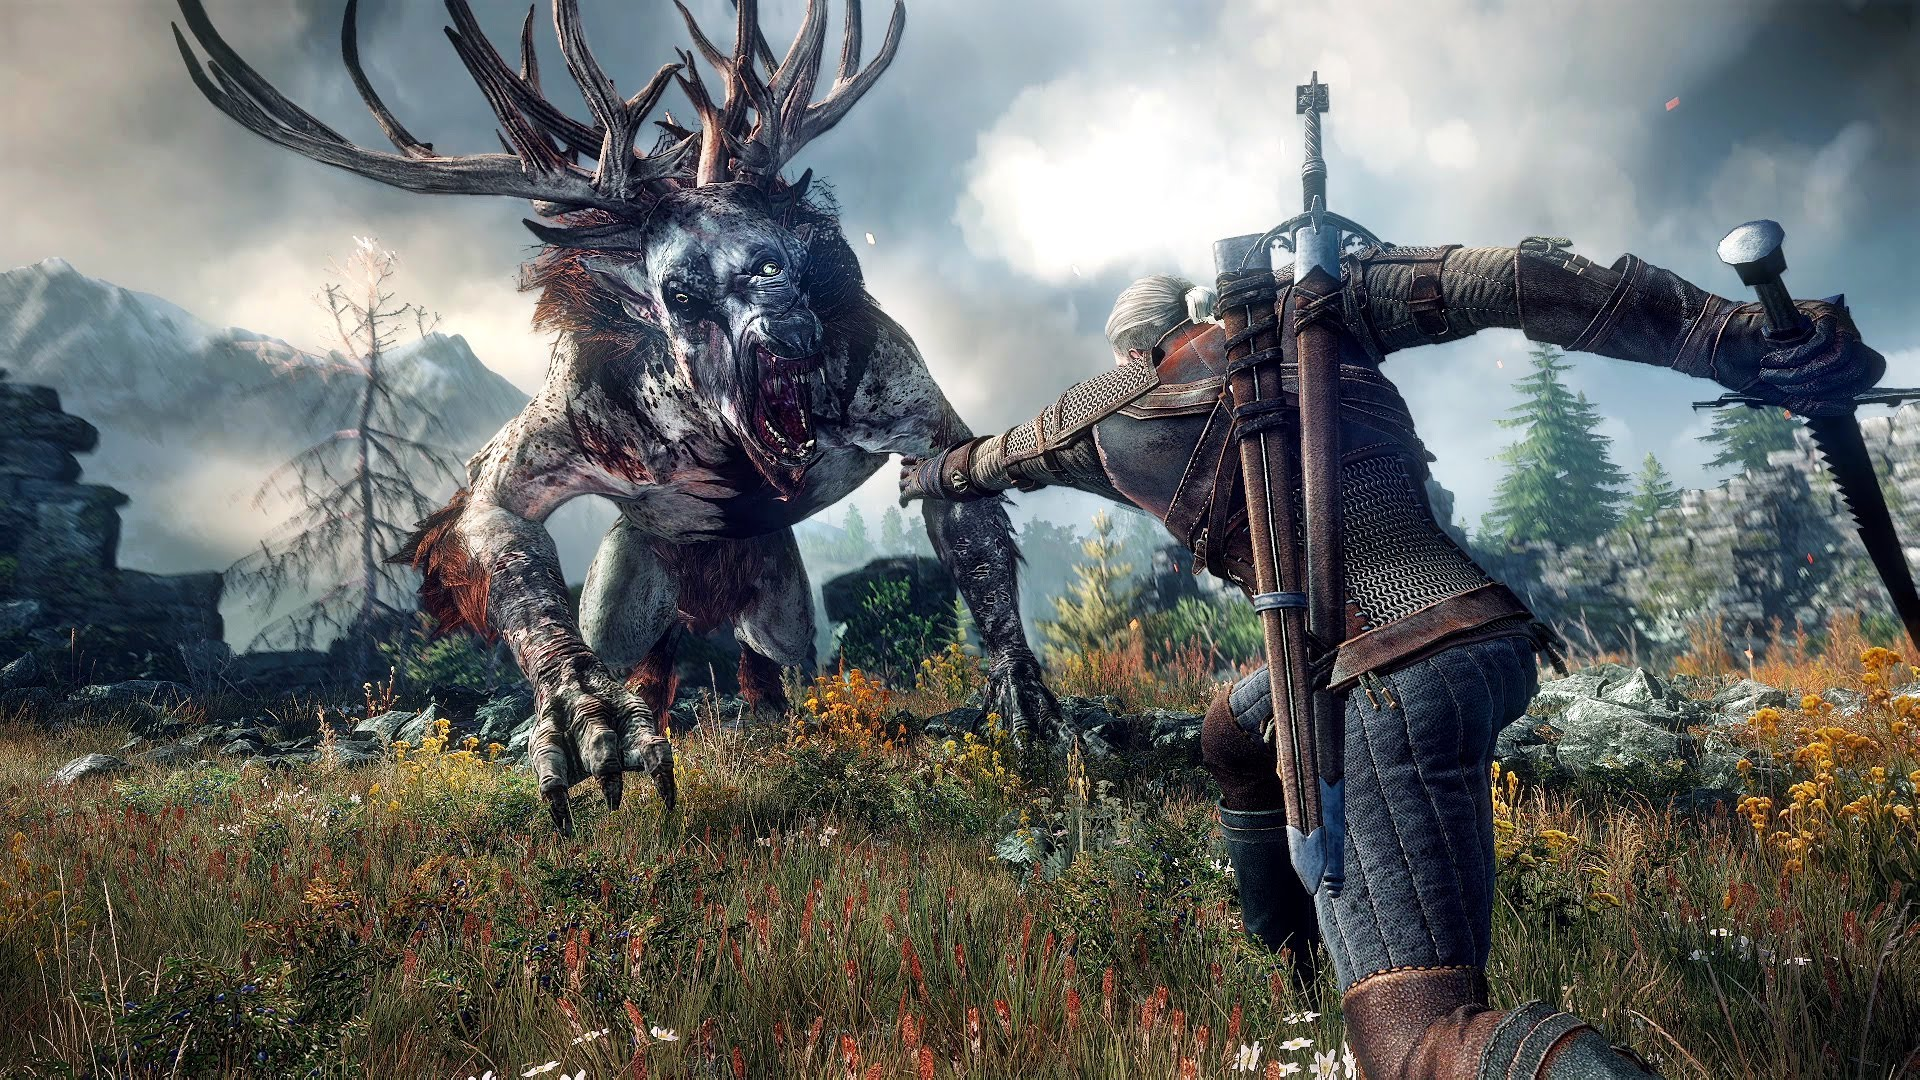
\includegraphics[scale=0.20]{img/whitcher.jpg}
	\caption{Contoh \textit{video game} dengan genre \textit{RPG}.}
	\label{fig:action_rpg}
\end{figure}
\vspace{1ex}

Pada dasarnya permainan dengan genre RPG (\textit{Role-Playing Game}) khususnya video game terbagi menjadi banyak kategori diantaranya adalah WRPG, JRPG, ARPG, TRPG, SRPG, dan MMORPG \citep{stenstrom2012}. Berikut adalah penjelasan selengkapnya:
\vspace{1ex}

\subsection{WRPG}
\label{sec:sub_sec2_wrpg}

Deskripsi tentang genre WRPG (\textit{Western Role-Playing Game}) ini diambil dari \textit{Dungeons and Desktops: The History of Computer-Role-playing Games} oleh Barton. Namun seperti yang direpresenatasikan oleh Barton menggunakan istilah CRPG, sedangkan dalam penelitian ini istilah WRPG yang akan digunakan.
\vspace{1ex}

Pada WRPG pemain dapat bebas mengkostumisasi karakternya dengan leluasa seperti jenis kelamin, wajah dan lain sebagainya. Kemudian pemain juga dapat memilih kemampuannya yang direalisasikan dalam bentuk atribut atau stats dari karakter pemain tersebut \citep{barton2019}. Pada umumnya hal yang dipilih oleh pemain biasanya berupa suku atau fraksi seperti pada \textit{video game} berjudul \textit{The Elder Scroll V: Skyrim}, Bethesda (2011) seperti pada Gambar \ref{fig:skyrim}.
\vspace{1ex}

\begin{figure} [!h] \centering
	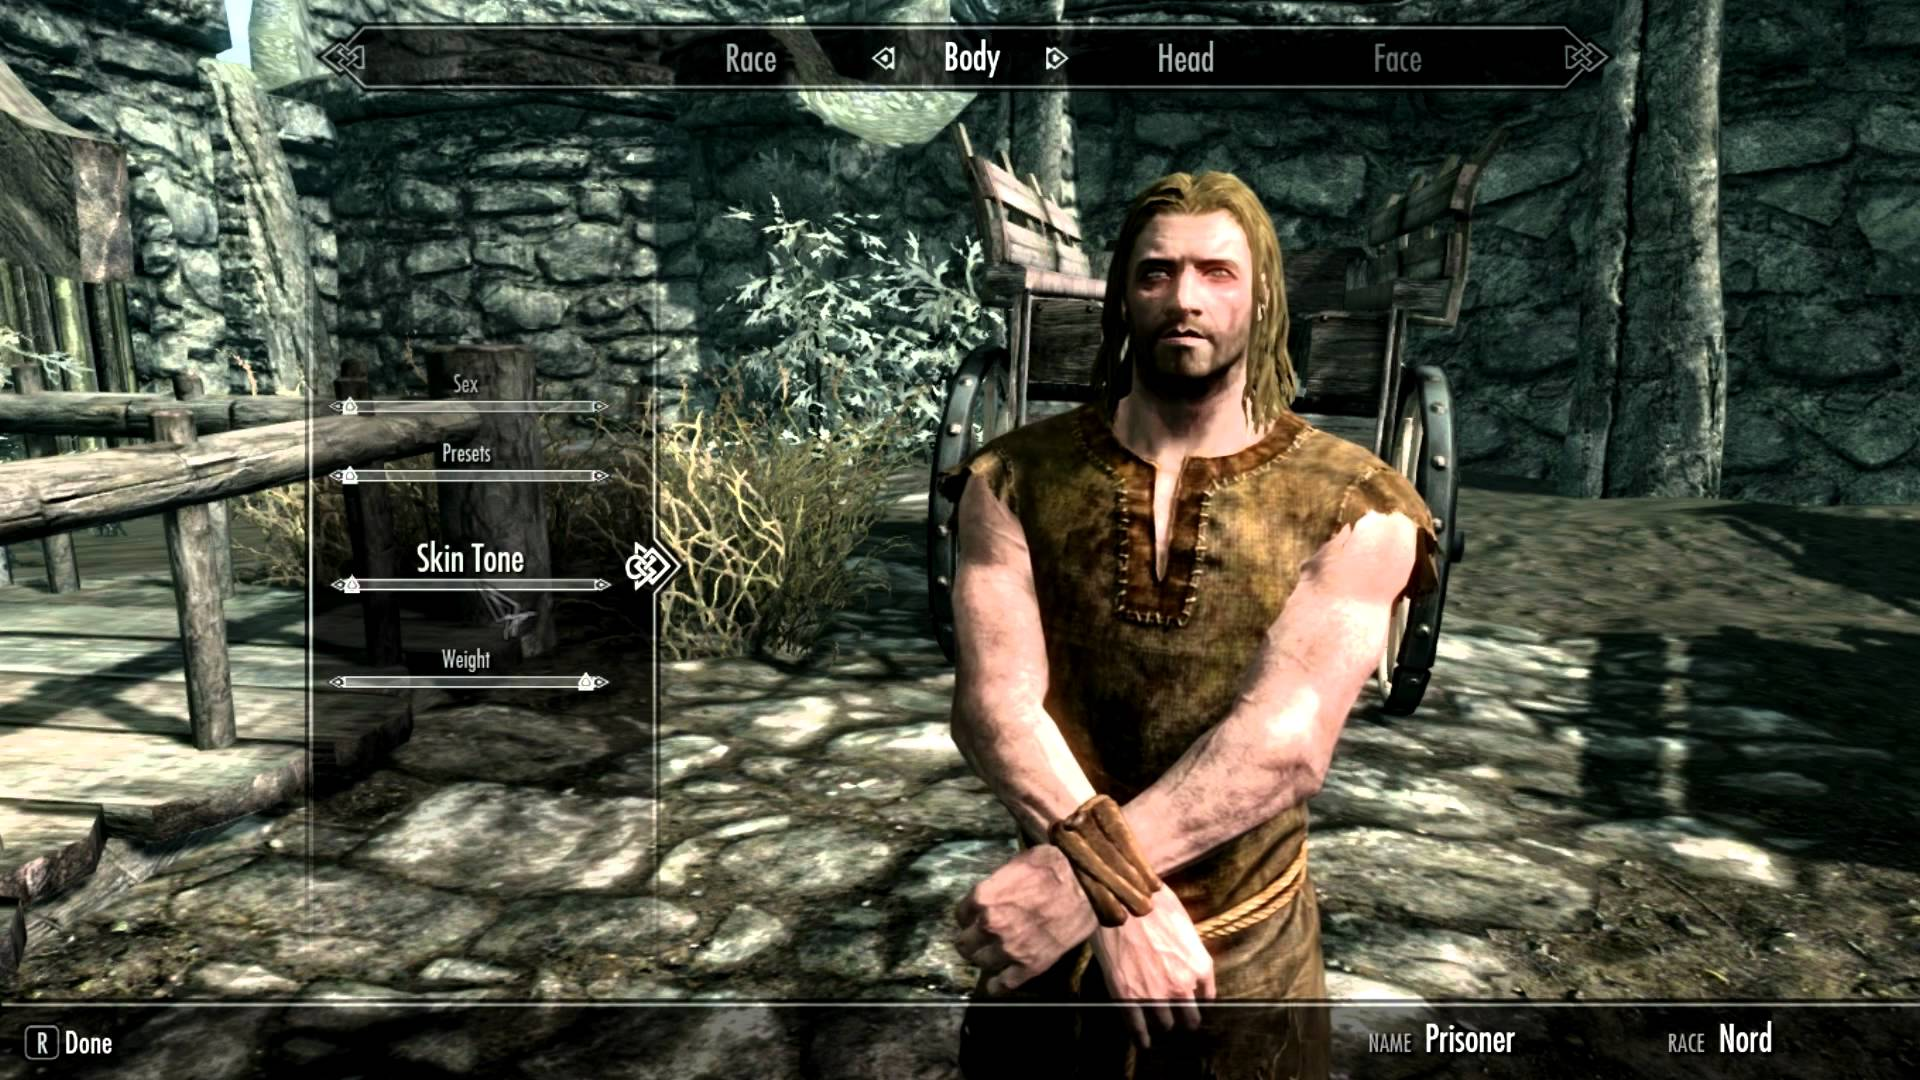
\includegraphics[scale=0.20]{img/skyrim.jpg}
	\caption{Contoh kustomisasi karakter pada WRPG.}
	\label{fig:skyrim}
\end{figure}

Sekumpulan musuh akan muncul sebelum permainan dimulai, dan pemain dapat menyiapkan perangkap atau membuat langkah kongkrit untuk mengalahkan sekumpulan  musuh tersebut. Sekumpulan musuh tersebut biasanya tersebar jumlahnya lebih banyak dari pemain. Atau mungkin pemain hanya berjumlah 1 dengan musuh yang berjumlah lebih dari itu, kemudian tugas dari pemain adalah mengalahkan sekumpulan musuh yang tersebar tersebut dengan melakukan pertarungan secara langsung atau \textit{real-time}, hal ini sangat identik dengan ARPG (akan dibahas pada poin selanjutnya).
\vspace{1ex}

Biasanya juga pada WRPG terapat banyak \textit{side quest} atau cerita sampingan yang berbeda dengan cerita utama. Hal ini memberikan pilihan jalan cerita untuk pemain dalam menyelesaikan permainan, selain itu karakter musuh dan juga boss dari musuh berbeda dengan misi atau cerita utama. Pada \textit{video game} berjudul \textit{The Witcher 3}, CD Pojekt (2015) memiliki banyak sekali cerita sampingan bahkan bisa dibilang cerita sampingan dari permainan tersebut tidak kalah bagusnya dengan cerita utama. Sekilas mengenai \textit{video game} berjudul \textit{The Witcher 3} dapat dilihat pada Gambar \ref{fig:action_rpg} pada bagian sebelumnya, saat dilakukan pertarungan secara \textit{real-time} melawan monster.
\vspace{1ex}

\subsection{JRPG}
\label{sec:sub_sec2_jrpg}

Pada mulanya permaian dengan genre JRPG (\textit{Japanese Role-Playing Game}) tidak begitu banyak mengandung kustomisasi karakter layaknya WRPG. Tetapi pada permainan RPG dengan genre ini berfokus pada beberapa karakter atau biasa disebut dengan istilah \textit{party member} yang dapat disusun oleh pemain. Sama seperti pada WRPG dimana pemain dapat mengkustomisasi kemampuan dari setiap \textit{party member} sesuai dengan peran masing-masing dengan tujuan untuk mengalahkan musuh. Dalam kostumisasi karakter pemain, biasanya diwujudkan dalam penambahan \textit{stats} dan penambahan jurus seperti pada \textit{video game} berjudul \textit{Shin Megami Tensei: Digital Devil Saga 1} dan \textit{2}, Atlus (2004, 2005) seperti yang ditunjukan pada Gambar \ref{fig:dds}.
\vspace{1ex}

\begin{figure} [!h] \centering
	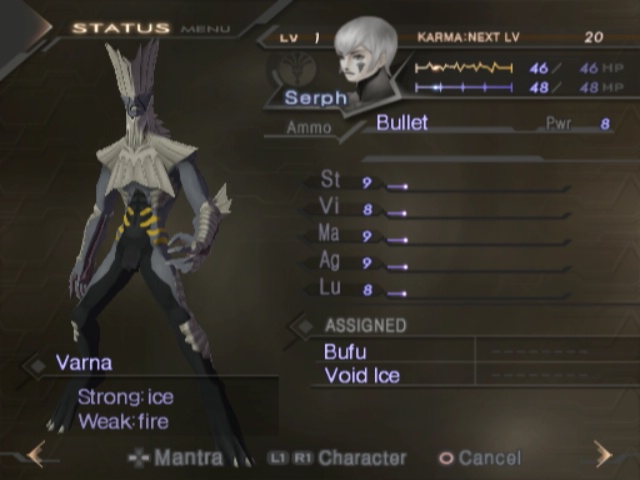
\includegraphics[scale=0.48]{img/dds.jpg}
	\caption{Contoh kustomisasi \textit{stats} pada JRPG.}
	\label{fig:dds}
\end{figure}

Pada mulanya pada permainan JRPG, pemain tidak mengetahui akan kedatangan musuh. Kedatangan musuh muncul secara tiba-tiba saat pemain melakukan pergerakan dalam peta permainan, hal ini biasa disebut denga istilah \textit{random encounter}. Contoh pada kondisi tersebut terdapat pada \textit{video game Shin Megami Tensei: Digital Devi Saga 1} dan \textit{2}. Jumlah musuh yang harus dilawan oleh \textit{party member} juga berjumlah lebih dari satu, sama-sama membentuk \textit{party member}.
\vspace{1ex}

Namun pada beberapa \textit{video game} JRPG, \textit{random encounter} juga direpresentasikan seperti monster atau bayangan yang mengejar representasi dari karakter pemain yang mewakili \textit{party member} dalam menjelajah dunia (eksplorasi). Setelah mereka bertabrakan maka terjadilah pertarungan antara \textit{party member} pemain dan musuh, seperti pada \textit{video game} berjudul \textit{Tales of Zestiria}, Bandai Namco (2015) dan juga \textit{Persona 4}, Atlus (2008).
\vspace{1ex}

Penataan strategi pada \textit{genre} JRPG bersifat sangat krusial, jika pada genre WRPG, ARPG dan SRPG pemain dapat mengganti perlalatan perangnya tetapi tidak pada genre JRPG. Pemain harus mempersiapkan segala seuatu dengan benar, apa saja yang dibutuhkan untuk mengalahkan musuh. Dalam mode pertarungan pada genre JRPG ada yang bersifat \textit{turn-based} seperti TRPG (akan dibahas pada poin selanjutnya) dan ada pula yang bersifat \textit{real-time} seperti WRPG.
\vspace{1ex}

Permainan berbasis \textit{turn-based} \citep{Panumate2015} adalah permainan yang memanfaatkan waktu secara diskrit, yang mana alur dari permainan khususnya pertarungan terbagi menjadi beberapa bagian yang disebut dengan giliran. Pada setiap giliran, pemain akan memiliki waktu yang terbatas atau tidak terbatas dalam berpikir dalam membuat keputusan setiap langkahnya. Kemudian sistem dari permainan akan memproses tindakan dari pemain. Kemudian permainan dilanjutkan oleh pemain berikutnya atau musuh yang berupa AI akan melakukan giliran selanjutnya seperti pada Gambar \ref{fig:turn_based}.
\vspace{2ex}

\begin{figure} [!h] \centering
	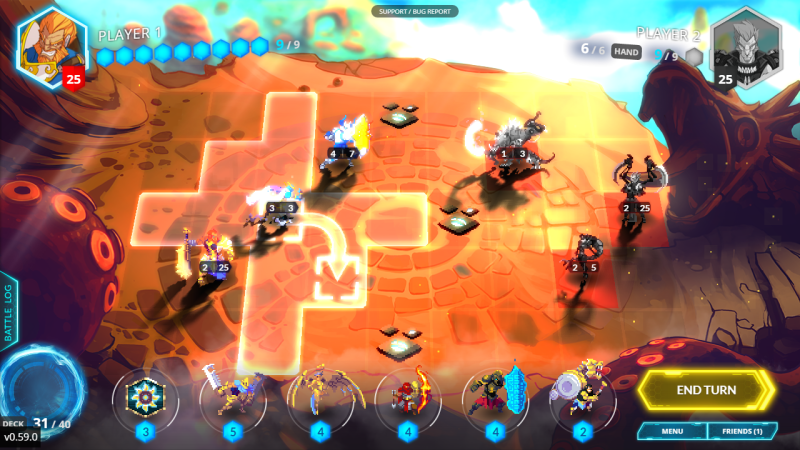
\includegraphics[scale=0.48]{img/duelyst.png}
	\caption{Contoh permainan digital dengan genre \textit{turn-based}.}
	\label{fig:turn_based}
\end{figure}

Pada Gambar \ref{fig:persona4} adalah mode pertarungan JRPG secara \textit{turn-based} yang dicontohkan oleh \textit{Persona 4}, Atlus (2008). Di mana para karakter yang dimainkan oleh pemain harus melakukan serangan secara bergatian yang kemudian baru dilanjutkan dengan serangan dari musuh.
\vspace{1ex}

\begin{figure} [!h] \centering
	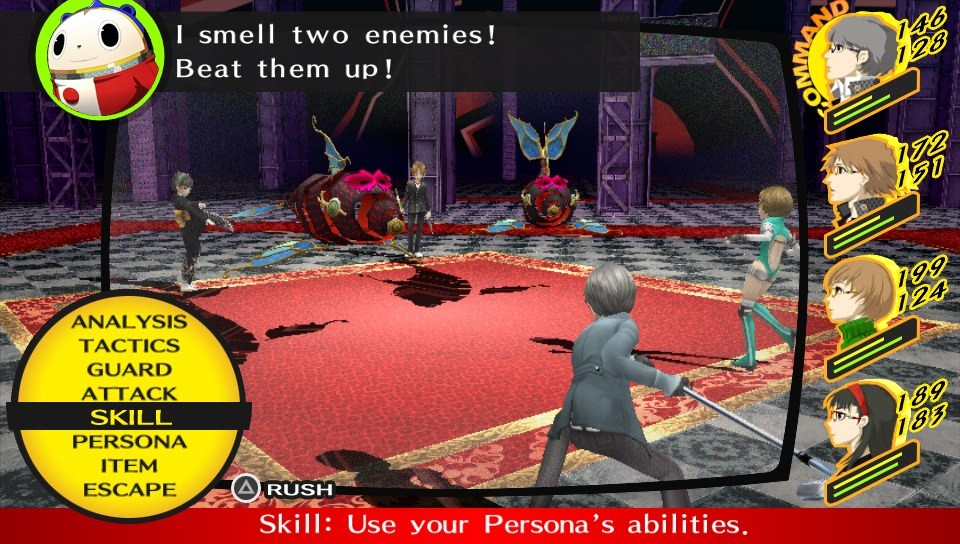
\includegraphics[scale=0.38]{img/persona4.jpg}
	\caption{Mode pertarungan \textit{turn-based} pada JRPG.}
	\label{fig:persona4}
\end{figure}

Pada Gambar \ref{fig:tales} adalah mode pertarungan JRPG secara \textit{real-time} yang dicontohkan oleh \textit{Tales of Zestiria}, Bandai Namco (2015). Di mana pemain menentukan formasi dalam party member, siapa saja karakter yang akan bertarung dan \textit{skill} apa saja yang dibutuhkan untuk mengalahkan musuh. Saat berlangsungnya pertarungan hanya satu karakter yang dapat dijalankan oleh pemain, tetapi pemain diberikan kelebihan untuk berganti karakter dalam pertarungan atau \textit{switch}.
\vspace{1ex}

\begin{figure} [!h] \centering
	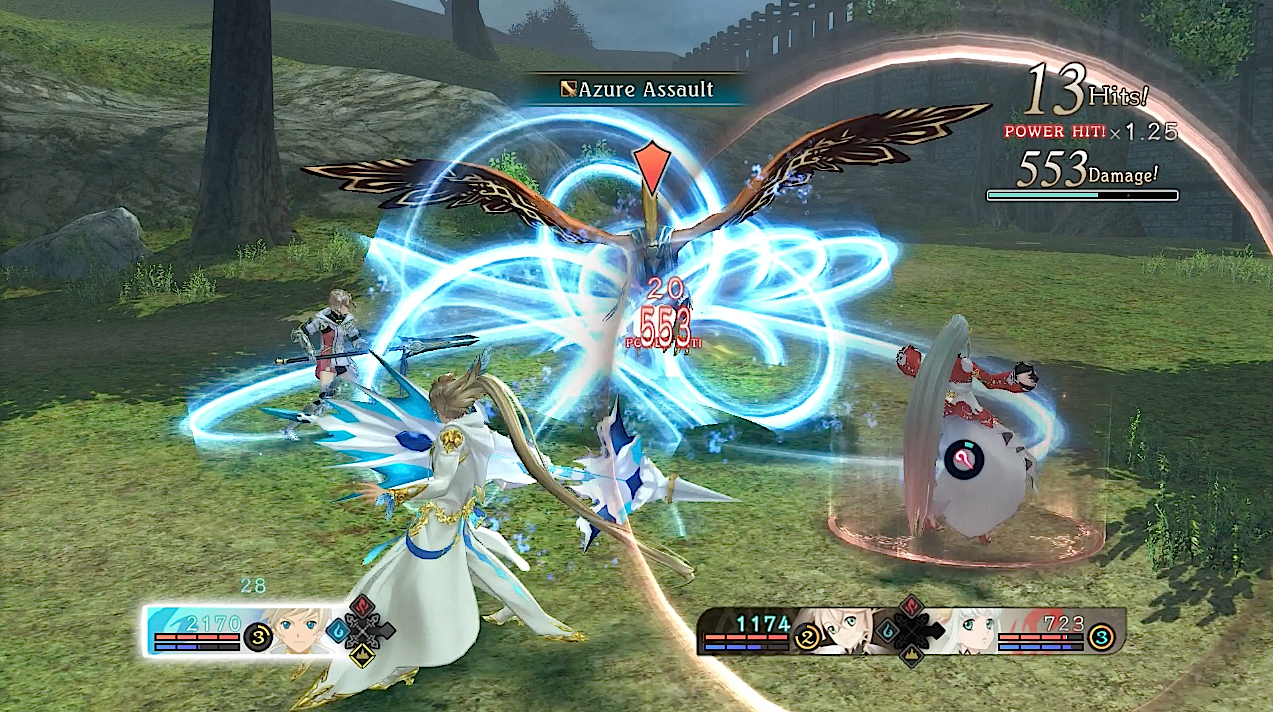
\includegraphics[scale=0.29]{img/tales.png}
	\caption{Mode pertarungan \textit{real-time} pada JRPG.}
	\label{fig:tales}
\end{figure}

Sama seperti dengan WRPG pada JRPG juga memiliki \textit{side-quest} tetapi biasanya hanya berupa permainan kecil saja, yang bersifat memainkan permainan lain diluar pertarungan antar \textit{party member}. Selain itu juga terdapat \textit{secret boss} yang bersifat sangat kuat dan sulit dikalahkan. Kemudian adanya \textit{new game+}, yang memungkinkan pemain untuk tetap memainkan karakter dengan kemampuan yang sama seperti permainan sebelumnya dan adanya penambahan konten untuk dimainkan (biasanya \textit{boss} yang lebih banyak).
\vspace{1ex}

\subsection{ARPG}
\label{sec:sub_sec2_arpg}

Biasanya genre ini disebut juga dengan ``\textit{Hack and Slash}'' atau ``\textit{Dungeon crawl RPG's}'' \citep{moore2016}. Kenapa sampai diberi sebutan ``\textit{Hack and Slash}'', hal ini mengacu dari kesederhanaan dari beberapa permainan ARPG. Pada permainan RPG jenis ini (khususnya \textit{video game}) berfokus pada aksi atau ketangkasan seperti memukul, menghindar, mengeluarkan jurus dan lain sebagainya dibandingkan dengan pengaturan strategi atau penyusunan \textit{stats}. Jika melihat cara bertarung pada permainan jenis ini, maka akan sangat mirip sekali dengan WRPG yang mana pemain fokus dalam bertarung dan berekplorasi. Contoh genre ini adalah \textit{Diablo}, Blizzard (1997) dan \textit{Final Fantasy 12}, Square Enix (2006).
\vspace{1ex}

\subsection{TRPG}
\label{sec:sub_sec2_trpg}

Pada RPG jenis ini tidak memiliki dunia atau maps yang digunakan untuk bereksploarsi sama sekali. Jadi pemain tidak perlu berkeliling sama sekali, sedangakan untuk sisi cerita pemain hanya melihat interaksi antar karakter atau interaksi antara karakter pemain dengan karakter musuh yang membentuk sebuah cerita.
\vspace{1ex}

Jumlah karakter yang dimainkan oleh pemain biasanya berjumlah sangat banyak dan terpapar dalam sebuah panel isometrik atau kotak, dan disanalah dilakukannya pertarungan antara karakter-karakter dari pemain melawan musuh-musuh. Pada RPG genre ini sangat berbanding terbalik dengan ARPG, yang mana pada TRPG sama sekali tidak membutuhkan aksi. Dalam artian tidak diperlukannya ketangkasan dalam melakukan serangan atau dalam menghindari serangan musuh, yang sangat diperlukan adalah 100\% perencanaan dan strategi. Pertarungan benar-benar dilakukan secara bergantian antara pemain dan musuh dalam melakukan serangan \citep{moore2016}. Contoh dari permainan dengan genre ini adalah \textit{Advance Wars}, Nintendo (2001). Penjelasan dari \textit{turn-based} atau bergantian sudah dijelaskan juga pada Sub-Bab \ref{sec:sub_sec2_jrpg} dan juga dicontohkan dengan \textit{video game} yang berjudul \textit{Duelyst}, Counterplay Games (2016).
\vspace{1ex}

Hampir sebagian besar permainan dengan genre ini berasal dari pengembang \textit{video game} asal jepang selayaknya JRPG. Terdapat juga versi lain TRPG, dengan adanya penambahan atribut \textit{speed} atau kecepatan yang menentukan karakter mana yang akan melakukan aksi terlebih dahulu. Contoh dari permainan tersebut terdapat pada \textit{Final Fantasy Tactics}, Square (1997).
\vspace{1ex}

\subsection{SRPG}
\label{sec:sub_sec2_srpg}

Genre RPG ini adalah termasuk yang paling modern, pada penelitian ini \textit{shooter} RPG dipersingkat menjadi SRPG. Biasanya istilah SRPG rancu dengan TRPG, yang mana S tersebut diartikan menjadi \textit{strategy}. SRPG sangat mirip sekali dengan ARPG hanya saja senjata utama dari permain ini menggunakan senapan atau panahan. Mengingat RPG jenis ini adalah \textit{shooter}, bukan berarti prespektif dari permainan ini adalah FPS (\textit{First Person Shooter}). Bisa jadi juga prespektifnya adalah \textit{third person} atau bahkan pemain bisa memilih mode yang mereka inginkan seperti pada \textit{video game} berjudul \textit{Fallout 4}, Bethesda (2015).
\vspace{1ex}

\subsection{MMORPG}
\label{sec:sub_sec2_mmorpg}

Kebanyakan \textit{gameplay} dari MMORPG (\textit{Masive Multiplayer Online Role-Playing Game}) terbagi menjadi dua jenis. Pertama adalah \textit{gameplay} yang mengedepankan kenaikan level dan selanjutnya adalah \textit{gameplay} yang mengedepankan penguatan karakter berdasarkan item yang dimiliki dalam memperankan perannya. Genre ini sangat mirip dengan WRPG dan JRPG, namun dijalankan secara \textit{online} atau daring yang mempertemukan banyak pemain dan terciptalah interaksi antar pemain yang diwakilkan dengan karakter yang dimainkan dalam permainan tersebut.
\vspace{1ex}

Permainan ini difokuskan pada interaksi sosial, dan perdagangan antar pemain, menciptakan perekonomian virtual, dan perusahaan virtual dari para pemain, yang biasa disebut persekutuan, grup, atau \textit{guilds}. \textit{Guilds} akan memiliki tujuan yang berbeda dalam permainan (\textit{Guilds} besar sering aktif dalam beberapa misi atau pertarungan), biasanya mereka akan fokus pada membersihkan \textit{dungeon} yang jauh lebih sulit yang mengharuskan banyak pemain atau anggota \textit{guilds} untuk ikut serta. Ini adalah alasan normal dari pemain untuk bergabung dengan \textit{guilds}, dengan menemukan para pemain pada waktu yang tepat, dan yang dapat memainkan peran dan permainan dengan baik. Hal itu akan menjadi sulit, jika tidak ada semacam jaringan atau penghubung antar pemain \citep{yeenick2020}. Contoh dari permainan MMORPG yang populer adalah \textit{World of Warcraft}, Blizzard Entertainment (2004) dan \textit{Ragnarok Online}, Gravity, Gravity Interactive (2002). 
\vspace{1ex}

Sistem pertarungannya adalah gabungan dari WRPG, JRPG, ARPG, dan TRPG. Namun pada umumnya MMORPG mirip dengan WRPG, terdapat pada bagian pembuatan karakter, dan pertempuran secara \textit{real-time} meskipun tidak benar-benar \textit{real-time}. Selain itu, terdapat beberapa permainan MMORPG yang memiliki pola permainan khas JRPG \citep{moore2016}, dengan banyaknya karakter yang dikendalikan oleh seorang pemain dan melakukan serangan sercara bergantian seperti \textit{Summoners War: Sky Arena}, Com2uS (2014) pada Gambar \ref{fig:sw}. Kemudian dengan adanya \textit{boss} dan banyak musuh dengan susunan dan kemampuan yang sudah terpola. Terdapat juga MMORPG dengan pertempuran yang sering kali mengharuskan para pemain untuk bergerak dan menghindari kemampuan musuh dan melakukan serangan disaat yang tepat seperti pada ARPG.
\vspace{1ex}

\begin{figure} [!h] \centering
	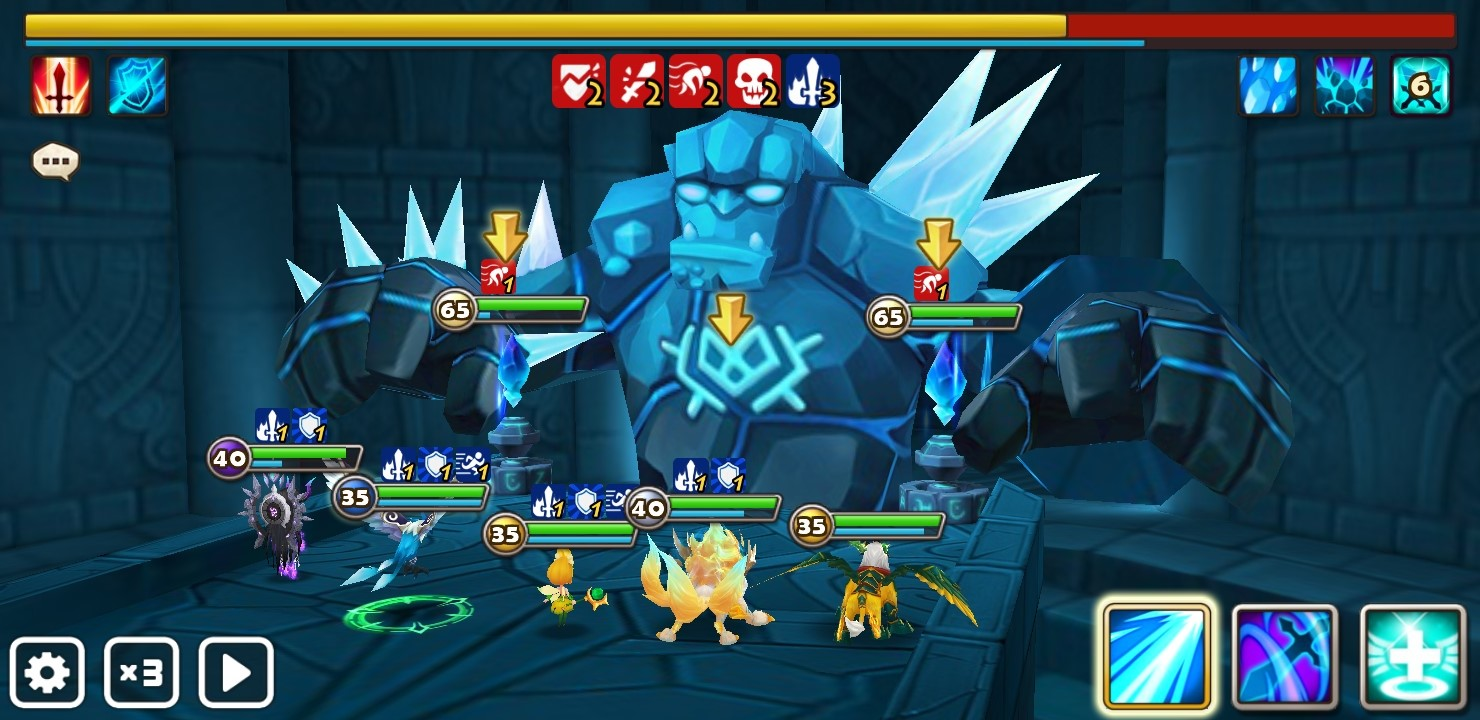
\includegraphics[scale=0.26]{img/sw.jpg}
	\caption{MMORPG yang menyerupai JRPG.}
	\label{fig:sw}
\end{figure}

Terakhir, permainan menyediakan fitur berupa pengembangan karakter dan perencanaan dari karakter yang dimainkan oleh para pemain, dan terlelih lagi mengharuskan pemain untuk melakukan perencanaan untuk bertarung bersama atau \textit{party} tetapi setiap pengguna hanya dapat memainkan satu karakter dalam \textit{party} tersebut, \textit{gameplay} tersebut sangat mirip dengan apa yang ditawarkan pada genre TRPG.
\vspace{1ex}

\section{Artificial Neural Network}
\label{sec:sec2_ann}
\vspace{1ex}

Terinspirasi dari cara kerja otak manusia dalam memproses informasi seperti yang ditunjukan pada Gambar \ref{fig:ann_neuron} \citep{buduma2017}, maka dibuatlah sebuah paradigma pemprosesan informasi yang biasanya digunakan untuk mempelajari tingkah laku sistem yang kompleks pada komputer, istilah ini biasa disebut dengan \textit{Artificial Neural Network}.
\vspace{1ex}

\begin{figure} [!h] \centering
	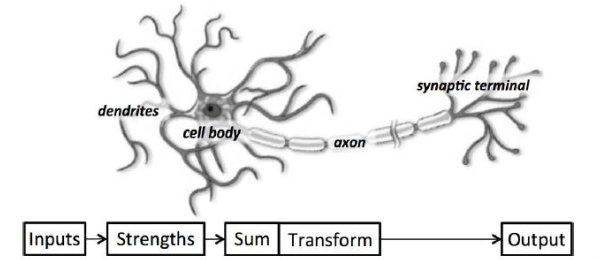
\includegraphics[scale=0.65]{img/ann_neuron.png}
	\caption{Skruktur neuron dan deskripsi fungsinya.}
	\label{fig:ann_neuron}
\end{figure}

Dengan mengiplementasikan cara kerja dari satu neuron dengan neuron yang lain yang diterapkan dalam program untuk komputer. Persamaan yang menyatakan perhitungan dari satu unit neuron adalah seperti yang ditujukan pada persamaan \ref{eq:ann_simple}.
\vspace{1ex}

\begin{equation}\label{eq:ann_simple}
y_{out} = wx_{in} + b
\end{equation}

Masukan skalar $x$ ditransmisikan melalui koneksi yang nilainya dikalikan oleh skalar beban atau \textit{weight} dengan $w$. Hasil perkalian tersebut ditambahkan dengan skalar bias yang dinyatakan dengan $b$. Proses tersebut menghasilkan luaran skalar yang dinyatakan dengan $y$, yang mana nilainya akan diteruskan ke neuron selanjutnya.
\vspace{1ex}

\subsection{Activation Function}
\label{sec:sub_sec2_activation_func}

\textit{Activation function} pada bertugas untuk menentukan apakah neuron tersebut harus aktif atau tidak, seperti neuron dalam otak manusia. Aktifasi neuron tersebut dipengaruhi oleh jumlah $w$ dari masukan. Secara umum terdapat 2 jenis \textit{activation function} yaitu linear dan non-linear.
\vspace{1ex}

Pada dasarnya \textit{activation function} dari sebuah neuron adalah Linear. Jika sebuah neuron menggunakan fungsi linear, maka keluaran dari neuron tersebut adalah $w$ dari $x$ + $b$. Pada Gambar \ref{fig:ann_linear} adalah contoh keluaran dari sebuah fungsi linear.
\vspace{1ex}

\begin{figure} [!h] \centering
	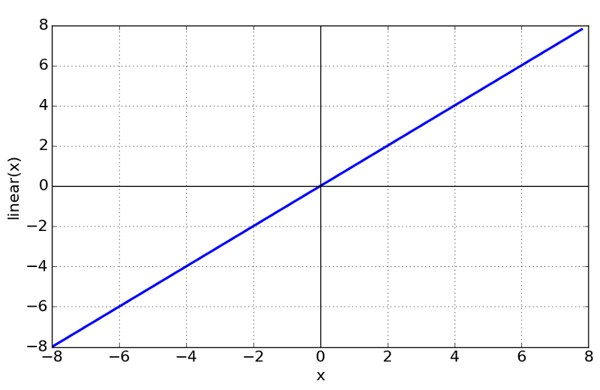
\includegraphics[scale=0.35]{img/ann_linear.jpeg}
	\caption{Output fungsi linear}
	\label{fig:ann_linear}
\end{figure}

Fungsi sigmoid mempunyai rentang antara 0 hingga 1 sedangkan rentang dari Tanh adalah -1 hingga 1. Kedua fungsi ini biasanya digunakan untuk klasifikasi dua kelompok data. Kemudian pada ReLU biasanya dilakukan \textit{treshold} dari 0 sampai dengan tidak terhingga. Pada Gambar \ref{fig:ann_non_linear} \citep{buduma2017} adalah contoh keluaran dari sebuah fungsi non-linear, yang masing-masing secara berurutan dengan (a) adalah Sigmoid, (b) adalah Tanh, dan (c) adalah ReLU.
\vspace{1ex}

\begin{figure} [!h] \centering
	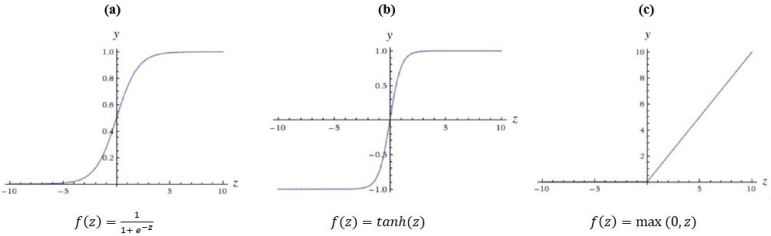
\includegraphics[scale=0.68]{img/ann_non_linear.png}
	\caption{Contoh fungsi aktivasi.}
	\label{fig:ann_non_linear}
\end{figure}

Kemudian terdapat sebuah activation function lagi yang akan digunakan pada penelitian ini, yaitu Softmax. Pada suatu kondisi akan dibutuhkan hasil klasifikasi yang berupa vektor dengan label atau kategori yang masih saling berhubungan. Contohnya saat penggunaan Neural Network dalam mengenali tulisan tangan yang berupa angka pada dataset MNIST. Hasil prediksi yang berupa angka atau label (0 sampai 9) yang masih saling terhubung, seperti kecilnya kemungkinan sebuah tulisan tangan angka dikenali dengan tingkat keyakinan 100\%. Maka digunakanlah probabilitas distribusi sehingga setiap label masih memiliki tingkat keyakinan masing-masing \citep{buduma2017}.
\vspace{1ex}

\subsection{Arsitektur Neural Network}
\label{sec:sub_sec2_nn_arch}

Arsitektur pada Gambar \ref{fig:ann_arch} biasa disebut sebagai \textit{Multi Layer Perceptron} (MLP) atau \textit{Fully-Connected Layer}. Arsitektur tersebut mempunyai 3 buah neuron pada \textit{input} Layer dan 2 buah \textit{node} pada \textit{output Layer}. Di antara \textit{input} dan \textit{output}, terdapat 1 \textit{hidden layer} dengan 4 buah neuron seperti yang ditunjukan pada Gambar \ref{fig:ann_arch}. Setiap neuron pada MLP saling berhubungan yang ditandai dengan tanda panah pada gambar diatas. Tiap koneksi memiliki \textit{weight} yang nantinya nilai pada setiap \textit{weight} akan berbeda-beda. \textit{Hidden layer} dan \textit{output layer} memiliki tambahan \textit{input} yang biasa disebut dengan bias. Sehingga pada arsitektur pada Gambar \ref{fig:ann_arch} terdapat 3 $\times$ 4 \textit{weight} + 4 \textit{bias} dan 4 $\times$ 2 \textit{weight} + 2 \textit{bias}. Total keseluruhan terdapat 26 parameter yang pada proses \textit{training} akan mengalami perubahan demi memperoleh hasil yang terbaik.

\begin{figure} [!h] \centering
	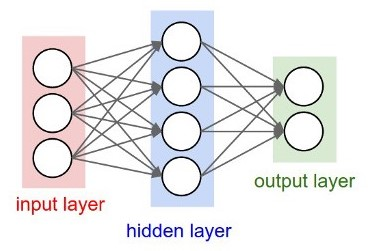
\includegraphics[scale=0.7]{img/ann_arch.jpeg}
	\caption{Contoh arsitektur sederhana \textit{Neural Network}.}
	\label{fig:ann_arch}
\end{figure}

Kemudian neuron pada \textit{input} layer tidak memiliki \textit{activation function}, sedangkan neuron pada \textit{hidden layer} dan \textit{output layer} memiliki \textit{activation function} yang kadang berbeda tergantung daripada data atau problem yang ingin diselesaikan.
\vspace{1ex}

\subsection{Training pada Neural Network}
\label{sec:sub_sec2_nn_train}

Pada \textit{Supervised Learning} menggunakan \textit{Neural Network}, pada umumnya proses \textit{learning} terdiri dari 2 tahap, yaitu \textit{training} dan \textit{evaluation}. Namun kadang terdapat tahap tambahan yaitu \textit{testing}, namun sifatnya tidak wajib. Dalam tahapan \textit{training} setiap \textit{weight} dan \textit{bias} pada tiap neuron akan diupdate terus menerus hingga \textit{output} yang dihasilkan sesuai dengan harapan. Pada tiap iterasi akan dilakukan proses \textit{evaluation} yang biasanya digunakan untuk menentukan kapan harus menghentikan proses \textit{training} atau stopping point. Secara garis besar proses training terdiri dari dua tahap sebagai berikut.

\begin{enumerate}[label=\textbf{\alph*.}]
	\item \textbf{\textit{Forward Pass}}: \textit{Forward pass} atau biasa disebut \textit{forward propagation} adalah proses dimana data dibawa dari input melewati setiap neuron pada \textit{hidden layer} sampai kepada \textit{output layer} yang nanti akan dilakukan perhitungan \textit{error}.
	\
	\item \textbf{\textit{Backward Pass}}: \textit{Error} yang didapat pada \textit{forward pass} akan digunakan untuk mengupdate setiap \textit{weight} dan \textit{bias} dengan \textit{learning rate} tertentu.
\end{enumerate}

Kedua proses tersebut dilakukan secara berulang-ulang sampai didapatkan nilai \textit{weight} dan \textit{bias} yang dapat memberikan nilai \textit{error} sekecil mungkin pada \textit{output layer} (saat \textit{forward pass}). Bila digambarkan maka akan menjadi seperti pada Gambar \ref{fig:ann_backpro} dengan panah biru adalah \textit{forward pass} dan panah merah adalah \textit{backward pass}.

\begin{figure} [!h] \centering
	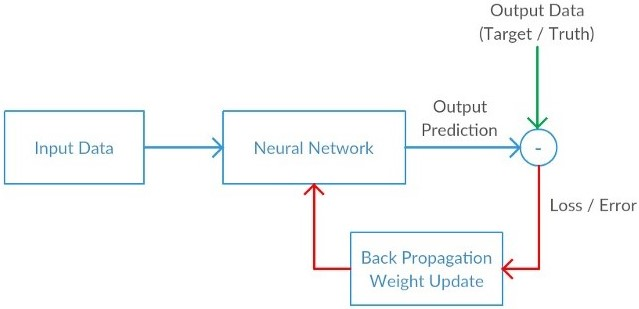
\includegraphics[scale=0.8]{img/ann_backpro.jpeg}
	\caption{Alur training untuk saat \textit{forward pass} dan \textit{backward pass}.}
	\label{fig:ann_backpro}
\end{figure}

Dalam \textit{Supervised Learning}, \textit{training data} terdiri dari \textit{input} dan \textit{output} atau target. Pada saat \textit{forward pass}, input akan dipropagasikan menuju \textit{output} layer dan hasil prediksi \textit{output} akan dibandingakan dengan target dengan menggunakan sebuah fungsi yang biasa disebut dengan \textit{Loss Function}. Maka untuk apa \textit{loss function} tersebut? Sederhananya loss function digunakan untuk mengukur seberapa baik performa dari \textit{Neural Network} yang dibuat saat melakukan prediksi terhadap target.
\vspace{1ex}

\begin{equation}\label{eq:ann_loss}
Loss = (Target - Predict)^{2}
\end{equation}

Pada persamaan \ref{eq:ann_loss} terdapat variabel $Target$ yang merupakan hasil yang diinginkan kemudian dikurangin dengan hasil prediksi yang dinyatakan denga $Predict$, maka diperolehlah $Loss$ atau tingkat kegagalan saat prediksi. Terdapat berbagai macam \textit{loss function}, namun yang paling sering digunakan adalah \textit{Squared Error} (L2 Loss) untuk regresi. Sedangkan untuk klasifikasi biasanya digunakan adalah \textit{Cross Entropy}.
	\cleardoublepage
	\chapter{METODOLOGI}
\label{chap:chap3_metodologi}

\section*{ }
Pada penelitian ini nantinya akan terdiri dari lima langkah utama yaitu analisa komponen permainan \textit{action} dan \textit{turn-based} RPG, desain level \textit{stats} atau data statisktik pada karakter pemain, desain level dan \textit{stats} pada setiap karakter musuh, dilanjutkan pengujian dengan berbagai parameter untuk stats pemain, kemudian dilakukan lagi pengujuin untuk validasi dengan \textit{deep learning mullticlass classification}. Di lanjutkan dengan beberapa langkah dibawahnya yang merupakan langkah-langkah detail dalam pengerjaanya seperti pada Gambar \ref{fig:metodologi_2}.

\begin{figure} [!h] \centering
	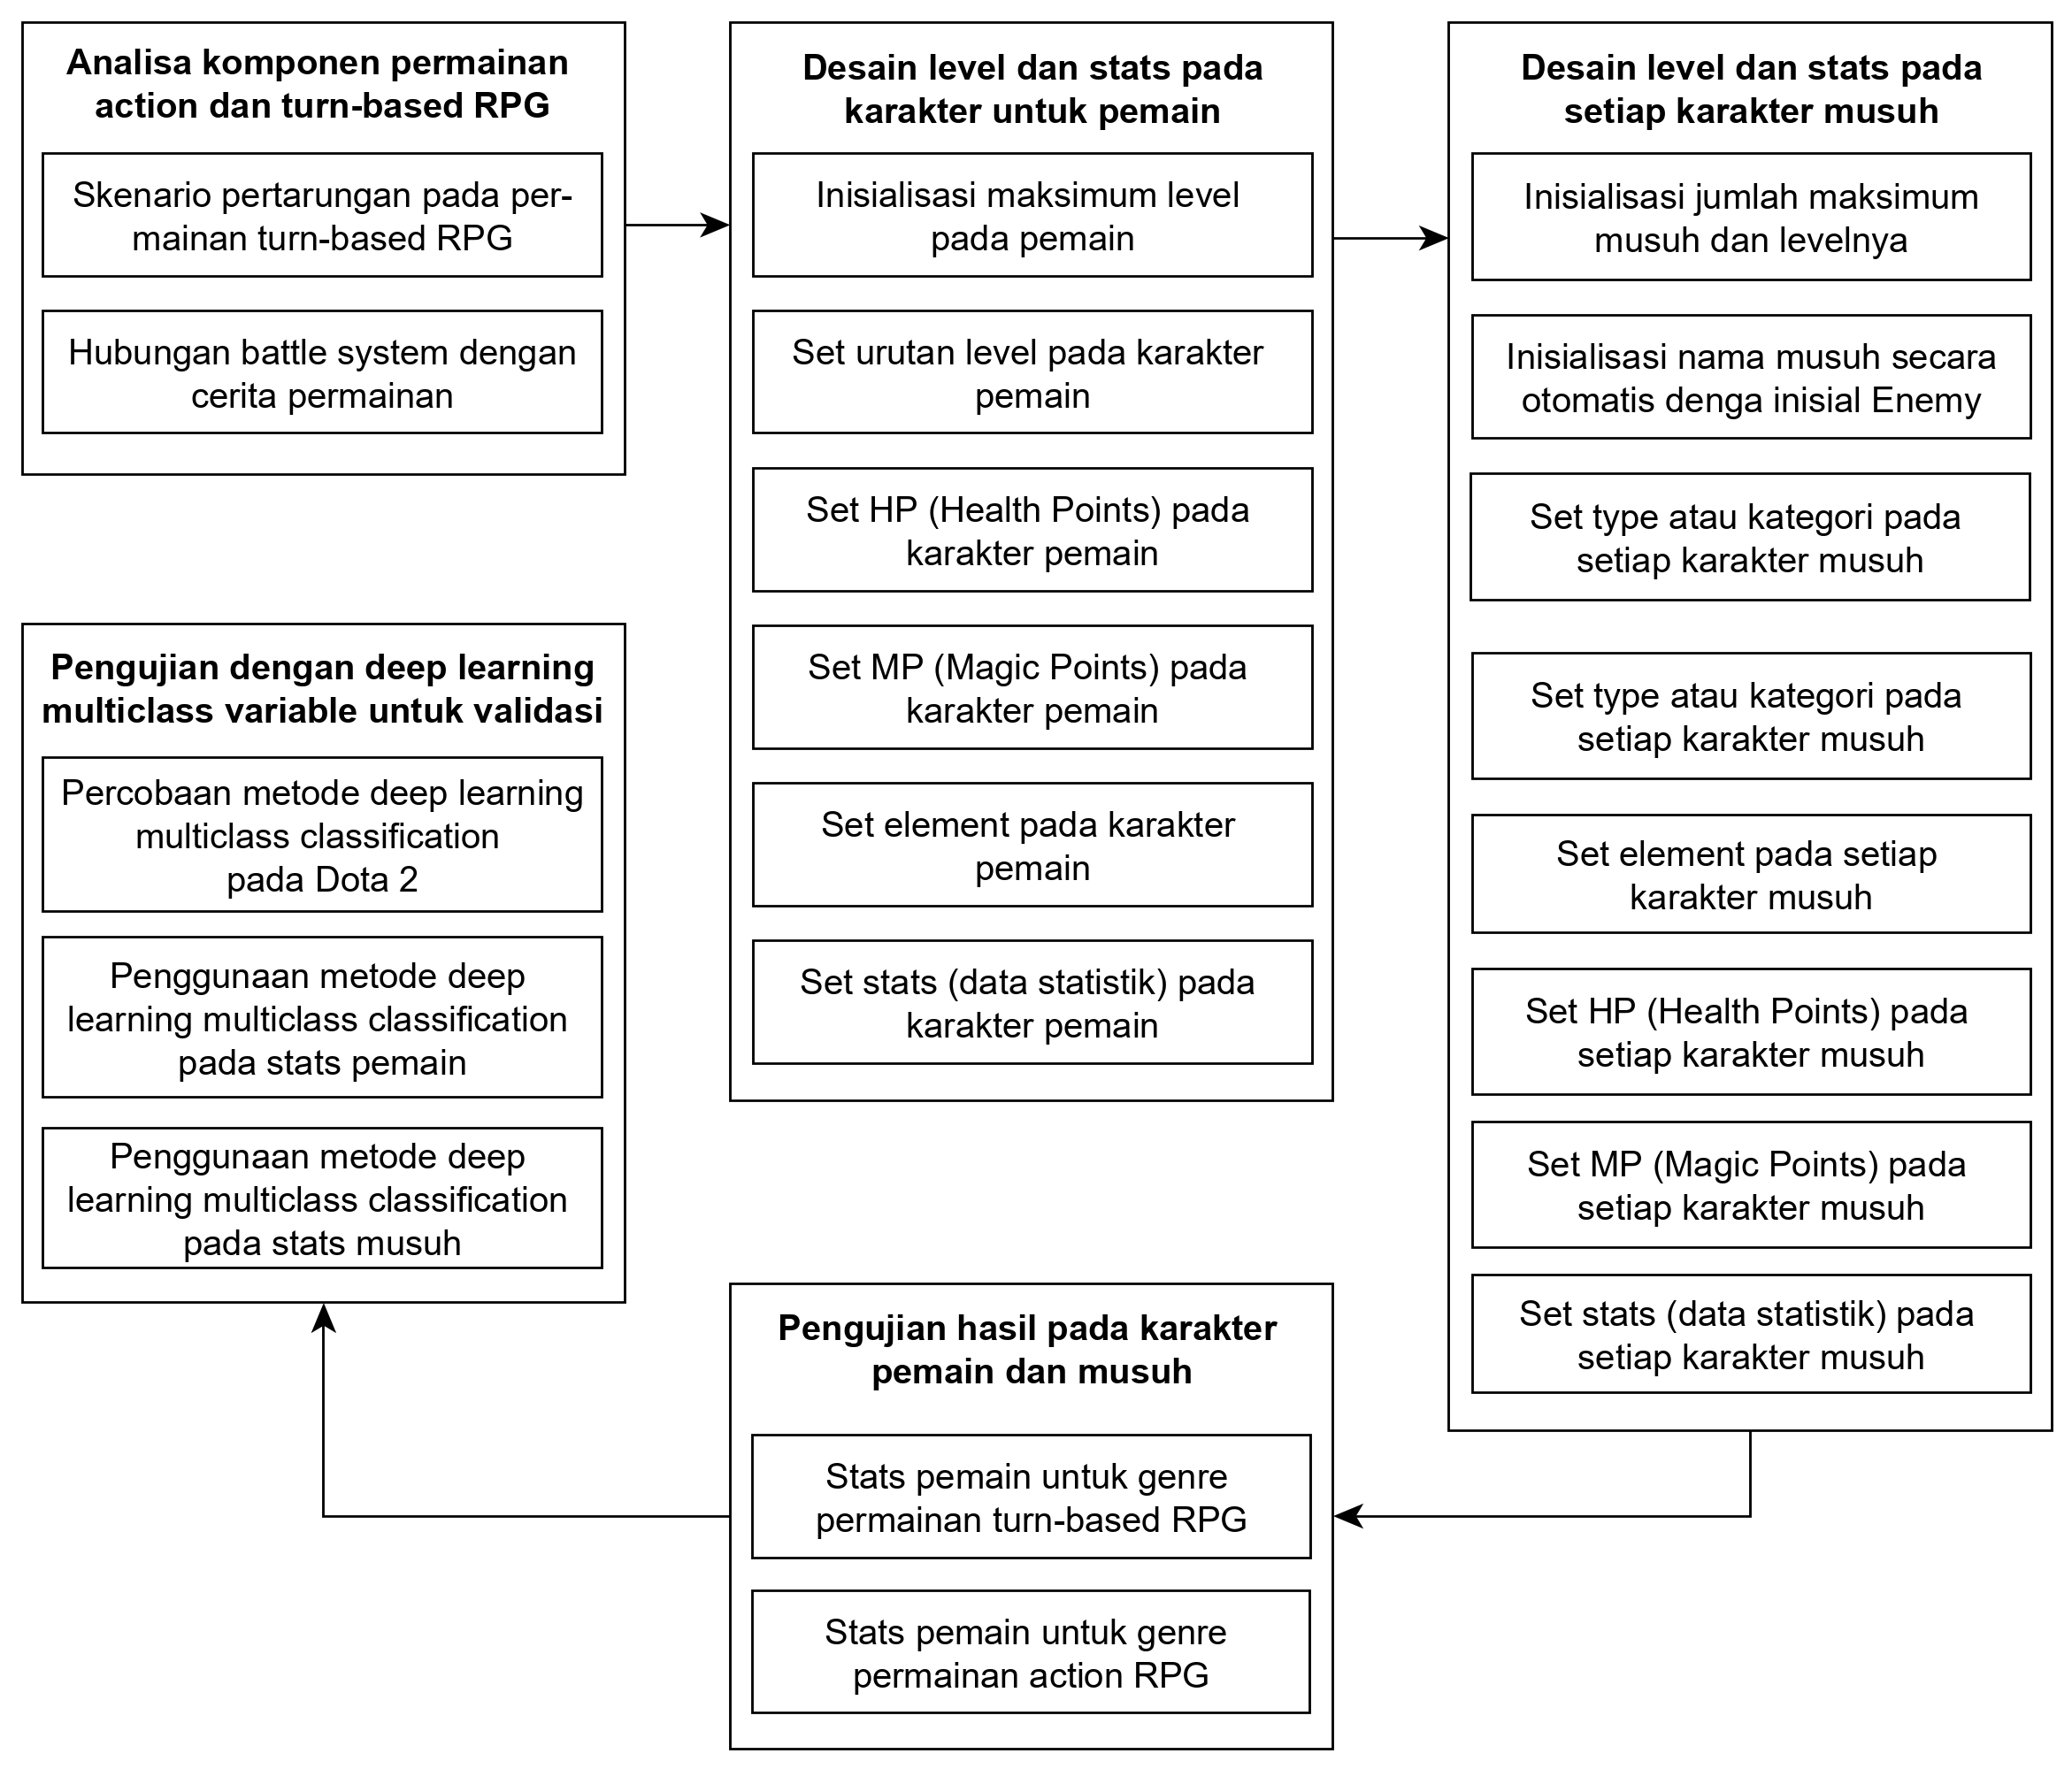
\includegraphics[scale=0.17]{img/metodologi_new.png}
	\caption{Urutan metodologi.}
	\label{fig:metodologi_2}    
\end{figure}

Tujuan umum dari penelitian ini adalah membuat \textit{stats} atau statistik untuk pemain dan musuh, sehingga dalam pembuatan permaian. Tujuan khusus dan fokus pada penelitian ini adalah untuk membuat data statistik untuk karakter pemain dan musuh dengan menggunakan metode $k-$NN dan \textit{Naive Bayes} yang kemudian dilakukan validasi dengan menggunakan metode \textit{Deep Learning} (\textit{Multiclass Classification}).
\vspace{1ex}

\section{Analisa Komponen Permainan Action dan Turn-based Role-Playing Game (RPG)}
\label{sec:sec3_design_komponen}
\vspace{1ex}

Pada bagian ini terdapat beberapa langkah yang akan menjelaskan penyusunan skenario pertarungan pada permainan RPG \textit{turn-based}. Pertama yang akan dilakukan adalah pembuatan skenario pertarungan pada permainan \textit{turn-based} RPG. Dari skenario tersebut tentunya harus ada hubungan dengan cerita dari permainan, apa saja parameter yang berpengaruh dari cerita terhadap skenario.
\vspace{1ex}

Di lanjutkan dengan desain level dan \textit{stats} dari pemain, selain itu digunakannya algoritma $k-$\textit{Nearest Neighbor} ($k-$NN) untuk mempercepat proses pembuatannya. Kemudian dilanjutkan dengan desain level dan \textit{stats} musuh yang juga dibuat secara otomatis dengan algoritma yang sama dengan pemain, namun tetap dipolakan oleh \textit{gaussian naive bayes} atau distribusi normal. 
\vspace{1ex}

Bagian selanjutnya adalah penambahan elemen pada pemain dan musuh yang membentuk kelebihan atau kekurangan pada masing-masing karakter. Pembagian elemen pada karakter yang dapat dimainkan oleh pemain dilakukan sesuai dengan cerita, sedangkan pembagian elemen pada musuh disebar secara acak berdasarkan \textit{stats} yang telah dibuat. Hal ini berkaitan erat dengan penjelasan pada Sub-bab \ref{sec:sub_sec2_kesempatan} tentang meningkatnya keberagaman, yang dibuktikan dengan banyaknya variasi musuh berikut dengan kelemahan dan kelebihannya.
\vspace{1ex}

\begin{subs}
	\subsection{Desain Skenario Pertarungan}
	\label{sec:sub_sec3_design_skenario}
	\vspace{1ex}
	
	Di umpamakan jumlah karakter yang rencananya akan digunakan berjumlah satu (\textit{action} RPG) sampai tiga karakter (\textit{turn-based} RPG) bergantung dengan alur cerita dari permainan dan jumlah musuh juga dimisalkan berjumlah antara satu sampai dengan enam, bergantung kepada tingkat kesulitannya seperti pada Gambar \ref{fig:battle_player}. 
	\vspace{1ex}
	
	\begin{figure} [!h] \centering
		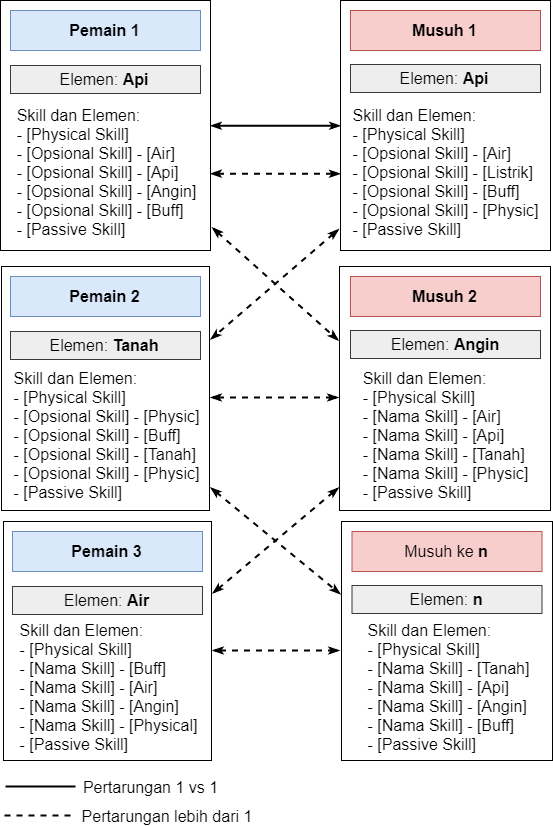
\includegraphics[scale=0.5]{img/battle_player_new.png}
		\caption{Skema pertarungan antar pemain.}
		\label{fig:battle_player}
	\end{figure}
	
	Sebelumnya pernah dijelaskan pada Sub-bab \ref{sec:sub_sec2_kesempatan} tentang meningkatnya pengambilan keputusan, pada kondisi semakin banyak musuh makan semakin banyak keputusan yang harus diambil oleh pemain. Selain itu setiap pemain memiliki elemen dan \textit{skill}, setiap elemen dapat menjadi kelemahan dan kelebihan dari setiap karakter. Hal tersebut akan membangun sebuah momen dramatis berdasarkan kompleksitas kombinasi dari musuh, hal tersebut dibahas pada Sub-bab \ref{sec:sub_sec2_kesempatan} tentang momen dramatis pada desain permainan.
	\vspace{1ex}
	
	Pada bagian ini dijelaskan contoh perancangan dari skenario pertarungan dengan genre \textit{action} dan \textit{turn-based} yang dibandingkan secara langsung. Pada Gambar \ref{fig:battle_player} jika dipecah dan dijelaskan lebih lanjut maka setiap karakter yang dimainkan oleh pemain atau musuh dalam bentuk NPC (\textit{Non Playable Character}) maka bagian-bagian tersebut akan menjadi seperti beberapa poin dibawah ini.
	\vspace{1ex}
	
	\begin{enumerate}[label=\textbf{\arabic*).}]
		
		\item \textbf{Stats}
		\setlength{\parindent}{0.8cm}
		
		\textit{Stats} atau statistik yang diperhitungkan dan berpengaruh dalam proses pertarungan. Pada Gambar \ref{fig:rpg_turn_based} ditunjukan tidak hanya karakter pemain saja, melainkan status dari pemain saat melakukan pertarungan. Pada Gambar \ref{fig:player_stats} adalah penggambaran dari komponen atau \textit{stats} pemain yang lebih detail seperti \textit{Health Point} (HP), \textit{Attack} atau serangan, \textit{Defense} atau pertahanan, \textit{Speed} atau kecepatan.
		\vspace{1ex}
		
		\begin{figure} [!h] \centering
			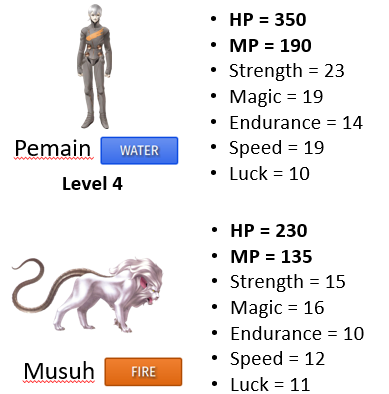
\includegraphics[scale=0.68]{img/player_stats.png}
			\caption{Status dari pemain pada permainan \textit{turn-based}.}
			\label{fig:player_stats}
		\end{figure}
		
		Berikut adalah penjabaran lebih dari beberapa komponen seperti HP, \textit{Attack}, \textit{Defense}, \textit{Speed} yang terdapat pada Gambar \ref{fig:rpg_turn_based}.
		
		\begin{enumerate}[label=\alph*).]
			\item \textbf{Health Point (HP)} adalah indikator nyawa atau kehidupan dari pemain, jika HP bernilai 0 maka karakter tersebut akan mati atu kalah.
			
			\item \textbf{Magic Point (MP)} adalah indikator jumlah dari jurus yang dapat dikeluarkan oleh pemain, jika MP bernilai 0 maka karakter tersebut tidak bisa mengeluarkan jurus atau kemampuan khusus.
			
			\item \textbf{Strength} adalah jumlah atau nilai serangan yang akan dilakukan untuk mengalahkan pemain lawan. Angka tersebut akan berlawanan atau dibandingkan dengan jumlah \textit{endurance} musuh. Hal tersebut bertujuan untuk mengurangi HP dari musuh.
			
			\item \textbf{Magic} atau \textit{Special Attack} biasanya tidak dimiliki oleh semua karakter pada permainan berbasis \textit{turn-based}. \textit{Special Attack} biasanya menjadi pembeda dalam setiap karakter berdasarkan jenis serangannya. Misalkan pada \textit{strength} biasanya berupa serangan fisik sedangkan pada \textit{special attack} berupa serangan \textit{magic} atau sihir.
			
			\item \textbf{Endurance} adalah jumlah atau nilai ketahanan yang digunakan oleh pemain atau musuh dalam menerima serangan. Hal ini bertujuan agar mencegah penurunan HP secara segnifikan, dengan membandingkan nilai serangan dengan nilai pertahanan.
			
			\item \textbf{Speed} atau kecepatan ada juga yang menyebutnya dengan \textit{agility} bertujuan dalam menentukan giliran dan keberhasilan dalam melakukan serangan. Semakin tinggi nilai \textit{speed}, biasanya semakin cepat melakukan serangan atau dapat mulai melakukan serangan lebih awal dibandingkan pemain atau musuh dengan nilai \textit{speed} yang lebih kecil.
			
			\item \textbf{Luck} atau keberuntungan adalah sebuah variabel yang digunakan menentukan hal yang bersifat acak, seperti bonus serangan atau \textit{critical attack}, kesempatan saat melakukan serangan balik atau \textit{counter attack} setelah diserang.
		\end{enumerate}
		
		Sementara itu skenario pertarungan dengan melibatkan \textit{stats} dijelaskan pada Gambar \ref{fig:battle_system} yang mana pemain atau musuh melakukan serangan berdasarkan \textit{speed}. Semakin tinggi \textit{speed} maka akan memperoleh giliran pertama untuk menyerang.
		\vspace{1ex}
		
		Di lanjutkan lagi dengan perhitungan dengan membandingkan \textit{Speed}, dan \textit{Luck} antara karakter pemain dengan musuh, pada proses tersebutlah yang menentukan apakah serangan dari pemain dapat diterima atau meleset terhadap musuh dan sebaliknya. Tingginya \textit{Speed} pada masing-masing karakter dapat diartikan perbandingn antara kecepatan untuk menyerang dan menghindar, sedangkan \textit{Luck} adalah faktor keberuntungan yang mempengaruhi serangan tersebut. Kemudian dilanjutkan lagi dengan kalkulasi \textit{attack} dan \textit{defense} antara karakter yang menyerang dan target. Dari hasil kalkulasi tersebut akan berpengaruh pada jumlah HP dari karakter yang menjadi target.
		\vspace{1ex}
		
		Kemudian pada permainan RPG dengan genre \textit{action} tidak membutuhkan skema berurutan serumit \textit{turn-based}. Pada permainan tersebut lebih mengandalkan ketangkasan dari pemain dalam memainkan karakter yang ingin dimainkan sepeti yang dijelaskan pada Sub-bab \ref{sec:sub_sec2_strategi} pada bagian pemain berbasis keterampilan sepenuhnya. Maka terjadilah momen saling serang secara langsung antara pemain dan musuh.
		\vspace{1ex}
		
		\begin{figure} [!h] 
			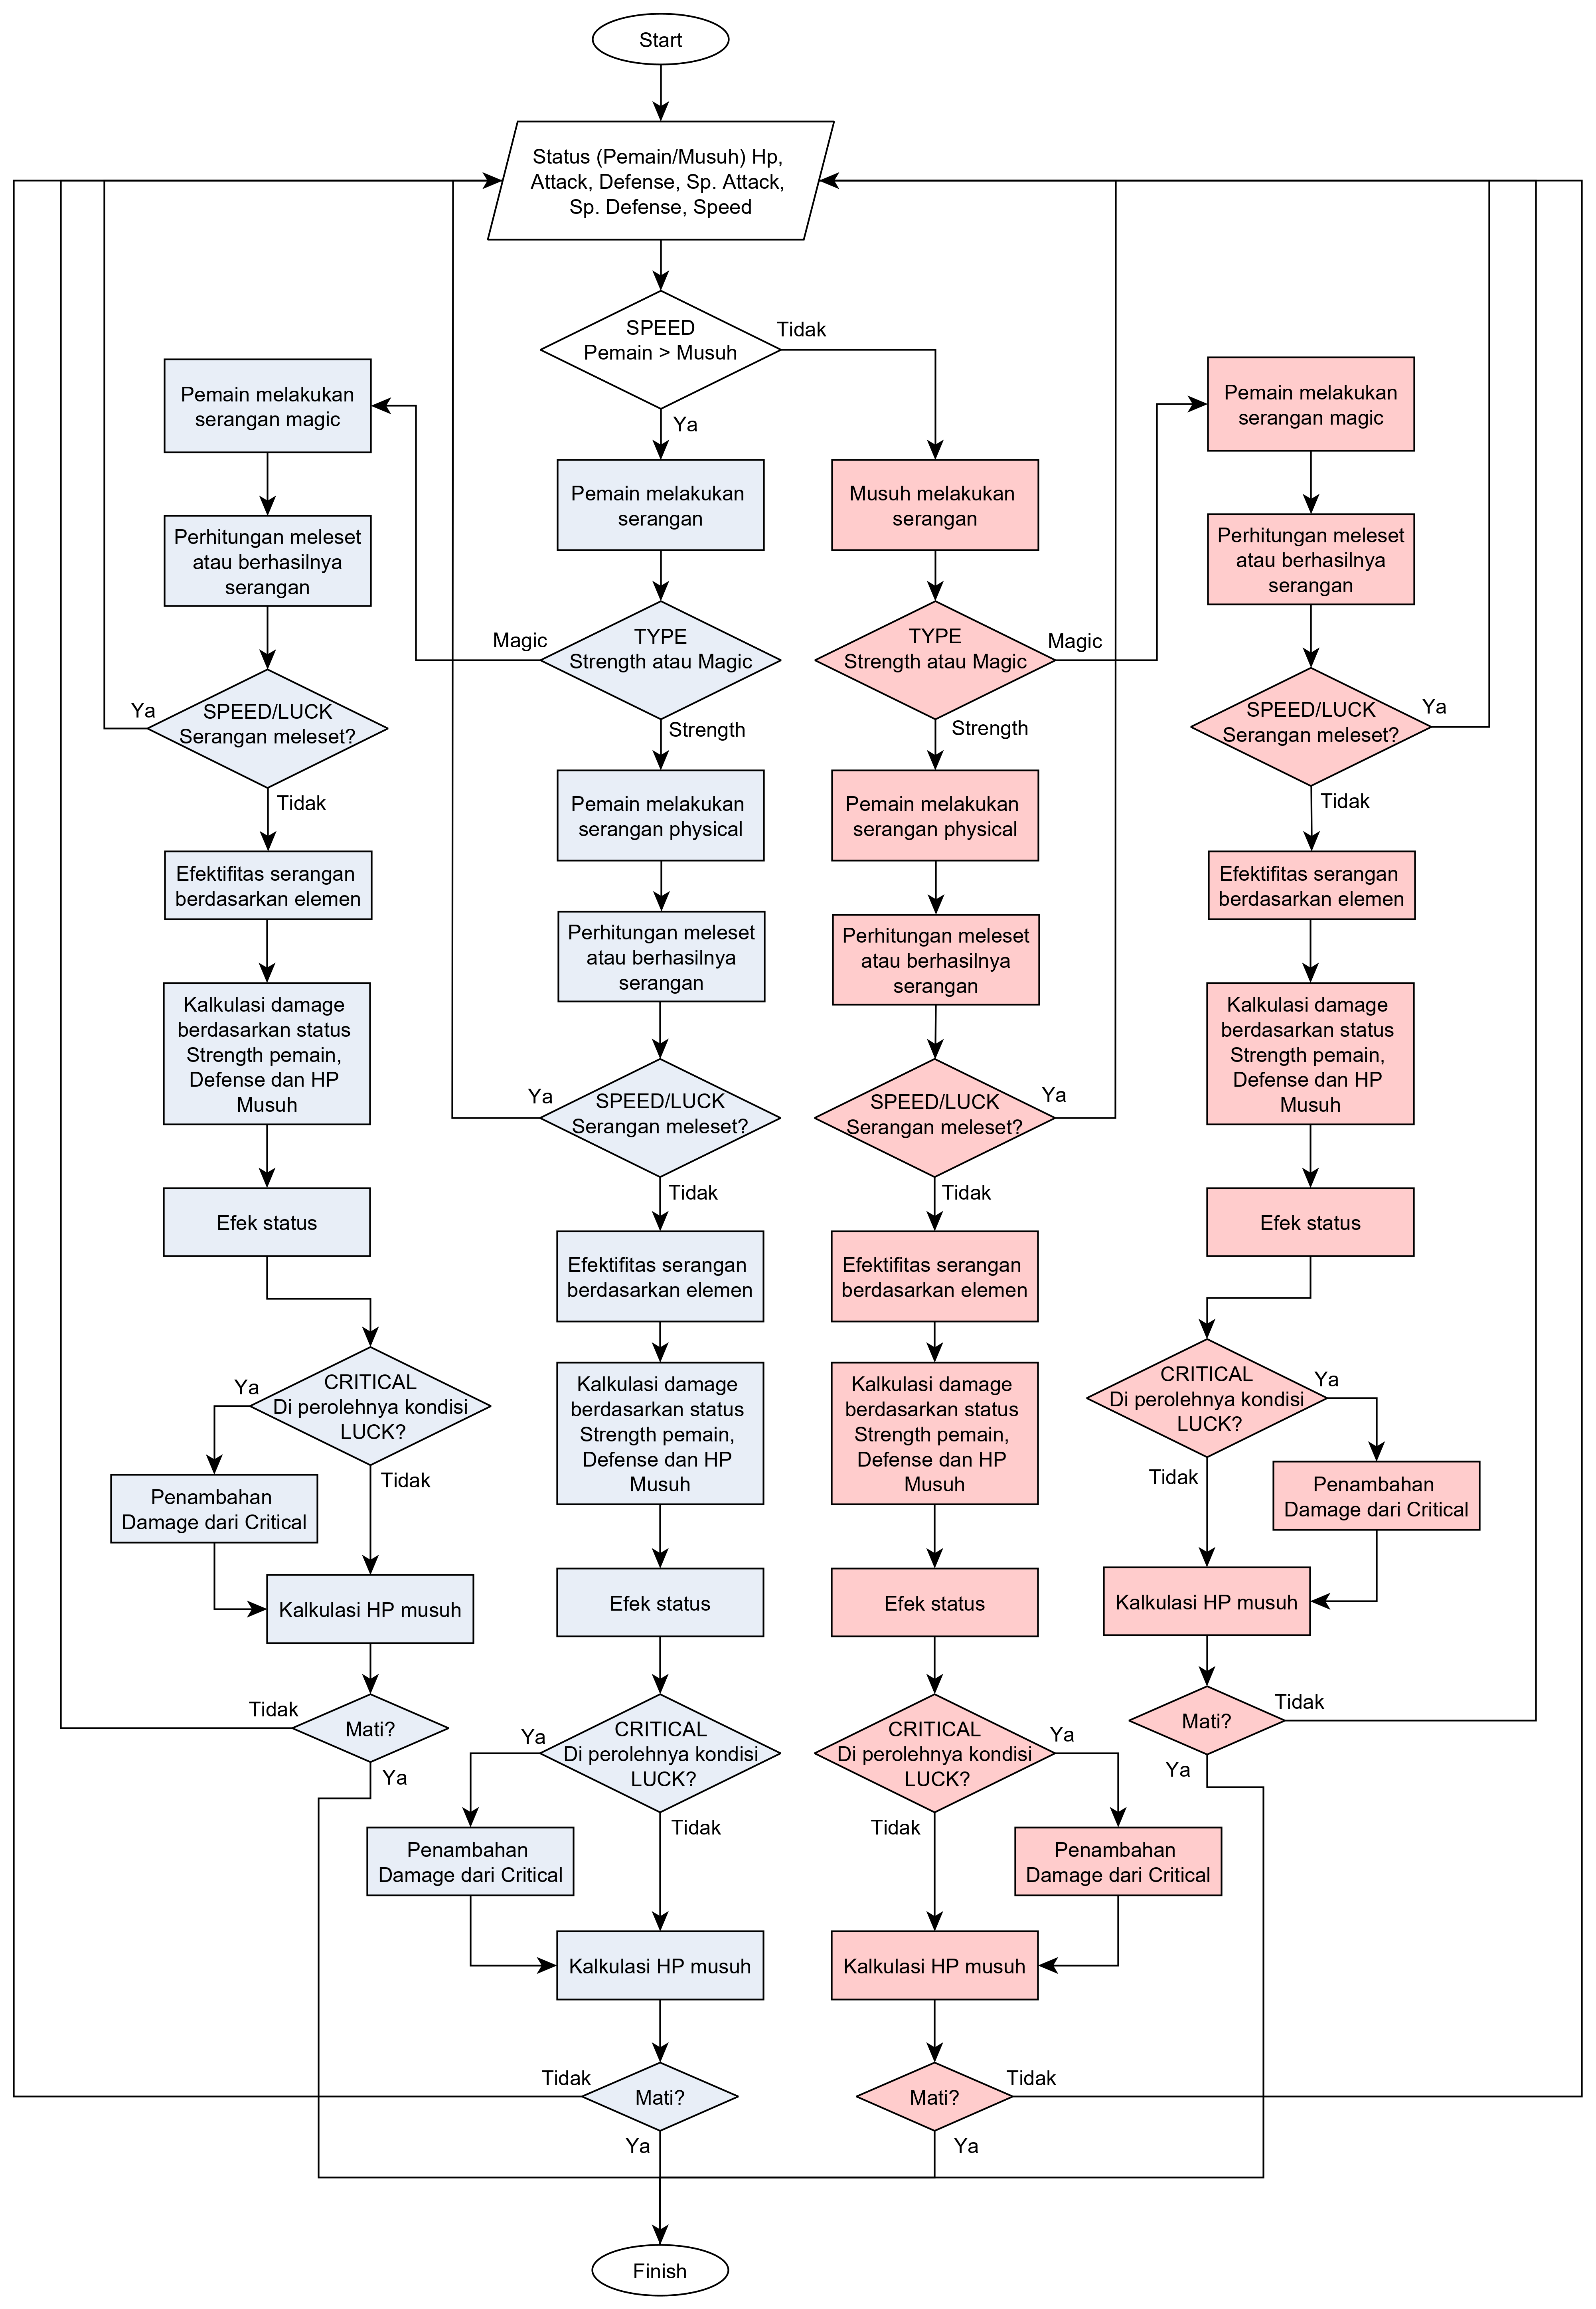
\includegraphics[scale=0.105]{img/battle_system_new_new.png}
			\caption{Skenario pertarungan \textit{turn-based}.}
			\label{fig:battle_system}
		\end{figure}
		\vspace{1ex}
		
		\item \textbf{Elemen dan Efektifitas Serangan}
		
		Pada Gambar \ref{fig:elemen} adalah contoh elemen yang digunakan dalam permainan dengan mode \textit{turn-based}. Jumlah dari elemen dapat ditambah atau dikurangi sesuai dengan kebutuhan. Biasanya jumlah dari elemen ditentukan berdasarkan cerita. Mengapa terdapat elemen tersebut, bagaimana asal-usulnya dan sebagainya seperti yang dijelaskan pada Sub-bab \ref{sec:sub_sec3_story}.
		\vspace{1ex}
		
		\begin{figure} [!h] \centering
			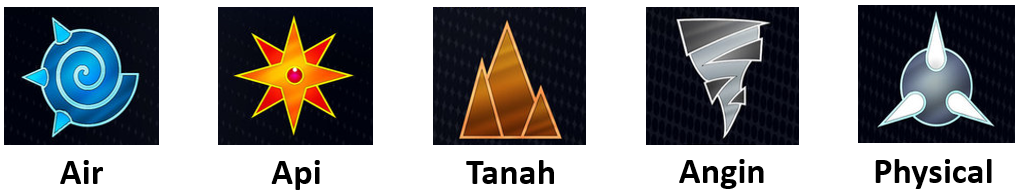
\includegraphics[scale=0.45]{img/element.png}
			\caption{Elemen pada permainan dengan mode pertarungan \textit{turn-based}.}
			\label{fig:elemen}
		\end{figure}
		
		Pembahasan ini mengacu kepada Gambar \ref{fig:battle_system} pada bagian ``efektifitas serangan berdasarkan elemen". Sedangkan pada Gambar \ref{fig:efektifitas} adalah perbandingan pengaruh atau keterkaitan sebuah elemen dengan elemen yang lain. Di mana setiap elemen memiliki kelemahan yang berupa elemen lain dan sebaliknya. Elemen-elemen tersebut saling berlawanan satu dengan yang lainnya sehingga mampu membentuk sebuah permainan yang membutuhkan strategi khusus. Kemudian dilanjutkan dengan perhitungan \textit{stats} seperti bagian sebelumnya.
		\vspace{1ex}
		
		\begin{figure} [!h] \centering
			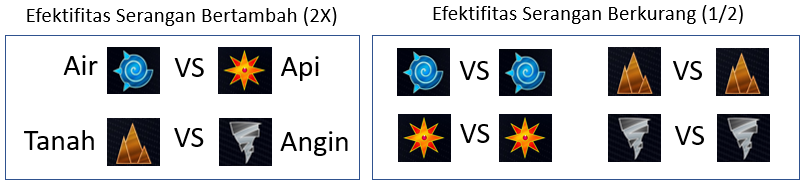
\includegraphics[scale=0.65]{img/efektifitas.png}
			\caption{Pengaruh elemen pada efektifitas serangan.}
			\label{fig:efektifitas}
		\end{figure}
		
		Jika melihat pada Gambar \ref{fig:efektifitas} dapat disimpukan bahwa beberapa element yang saling berlawanan kemudian efektifitas menjadi 2 kali lipat, contohnya pada elemen air terhadap api dan tanah terhadap angin begitu juga sebaliknya. Jika elemen yang sama saling bertarung maka efektifitasnya berkurang $1/2$ dari yang seharunya. Kemudian pada elemen lain yang belum disebutkan berlaku efektifitas normal atau 1 kali. Pembagian elemen pada pemain dan musuh akan dibahas lebih detail pada Sub-bab \ref{sec:sec3_player_stats}.
		\vspace{1ex}
		
		Kebanyakan elemen dan efektifitas serangan berlaku pada permainan RPG dengan genre \textit{turn-based}, berbeda halnya dengan \textit{action} yang lebih mengandalkan keterampilan dari pemain dalam memaikan karakternya seperti yang dijelaskan pada Sub-bab \ref{sec:sub_sec2_strategi} pada bagian pemain berbasis keterampilan sepenuhnya.
		\vspace{1ex}
		
		\item \textbf{Efek Status}
		
		Pada Gambar \ref{fig:battle_system} terdapat bagian ``efek status", maksud dari proses tersebut adalah penambahan efek yang merugikan terhadap pemain setelah diserang. Efek kerusakan dapat membawa kesan lebih taktis pada pertempuran. Berikut adalah efek status yang akan diterapkan pada sistem pertarungan.
		
		\begin{enumerate}[label=\alph*).]
			\item \textbf{Infected:} Karakter kehilangan 10\% dari total HP setiap giliran.
			
			\item \textbf{Confused:} Karakter tidak dapat dikendalikan dan mungkin akan bertahan, menyerang dan tidak melakukan apa-apa. Ada juga kemungkinan mereka akan berbalik menyerang \textit{party member} mereka sendiri.
			
			\item \textbf{Silence:} Karakter tidak dapat mengubah Personae atau menggunakan keterampilan Persona.
			
			\item \textbf{Tired:} Karakter kehilangan SP untuk setiap tindakan yang diambil, dan menerima lebih banyak \textit{damage} dari musuh ketika diserang.
			
			\item \textbf{Hacked:} Efek yang muncul setelah target diserang sesuai dengan kelemahannya. Target kemudian akan menerima lebih banyak \textit{damage} dan tidak dapat menghindar. Jika target diserang lagi, maka statusnya akan berubah menjadi disabled.
			
			\item \textbf{Disabled:} Target akan hilang 1 giliran untuk mengambil tindakan, kemudian mendapat lebih banyak kerusakan dan serangan tidak dapat dihindari.
		\end{enumerate}
		
		Tidak semua kemampuan pemain dapat memberi efek status, hal tersebut mengacu pada desain permainan yang mengatur keseluruhan \textit{skill}, tidak hanya pada karakter utama melainkan juga pada musuh. Tetapi dalam penelitian ini, hal tersebut masih belum terpakai dikarenakan masih menyelesaikan perihal desain \textit{stats} dari pemain dan musuh. Hal ini baru semacam perkiraan saja saat mendesain sebuah permainan.
		\vspace{1ex}
		
		Pada bagian efek status juga berlaku pada permainan RPG dengan genre \textit{action}, setelah berlangsungnya pertarungan antara pemain dan musuh. Di mana pada sisi pemain dapat memhangun karakternya sedemikian hingga demi memberi efek status ke pada musuh saat berlangsunnya pertarungan seperti yang dijelaskan pada Sub-bab \ref{sec:sub_sec2_strategi} tentang peran dan keterampilan pemain serta strategi dan taktik.
		\vspace{1ex}
		
		\item \textbf{Kondisi Kritis pada Serangan}
		
		Selain \textit{attack}, elemen dan efek status, masih terdapat \textit{damage} yang dapat ditimbulkan oleh penyerang kepada target yaitu kondisi kritis pada serangan. Dengan jumlah \textit{attack} ditambah dengan jumlah \textit{attack} yang dikalikan dengan presentase tingkat kondisi kritis (\textit{critical rate}) pada \textit{skill} yang dipilih untuk menyerang lawan. Kondisi tersebut didapat dengan membandingkan nilai \textit{stats} dari \textit{Strength} atau \textit{Magic} dan \textit{luck} milik penyerang dan target, pada proses tersebutlah yang menentukan apakah serangan tersebut diperoleh kondisi kritis atau tidak. Hal tersebut juga membangun sebuah momen dramatis berdasarkan peluang terjadinya kondisi kritis saat terjadinya serangan dari pemain terlebih lagi dari musuh seperti yang dibahas pada Sub-bab \ref{sec:sub_sec2_kesempatan} tentang momen dramatis.
		\vspace{1ex}
		
		\item \textbf{Kalkulasi HP dan MP}
		
		Pada akhirnya jumlah kerusakan yang ditimbulkan oleh penyerang dan HP dari target akan dikalkulasikan. Jika HP target habis atau sama dengan 0, maka terget tersebut dinyatakan mati. Dan jika HP target masih bersisa, maka pertarunggan akan dilanjutkan oleh giliran karakter dari pemain atau musuh selanjutnya. Kemudian pada sisi penyerang juga ada yang dikorbankan dalam upaya melakukan serangan. Saat penyerang memilih serangan fisik makan pemain akan mengorbanakan sebagian HP yang dimiliki, jika yang dipilih adalah serangan \textit{magic} maka yang dikorbankan adalah MP.
	\end{enumerate}
	
	\subsection{Hubungan Sistem Pertarungan dengan Cerita}
	\label{sec:sub_sec3_story}
	\vspace{1ex}
	
	Pada setiap permainan RPG khususnya \textit{action} dan \textit{turn-based} RPG pasti memiliki cerita yang menjadi latar belakang permainan seperti yang dijelaskan pada Sub-bab \ref{sec:sec2_turn_based_rpg}. Tentunya cerita tersebut juga memiliki pengaruh penting terhadap jumlah karakter yang dapat dimainkan oleh pemain, jumlah musuh, elemen apa saja yang akan dipakai, total waktu permainan, jumlah musuh yang harus dilawan dan lain sebagainya. Pada penelitian ini hal semacam itu akan dibuat menjadi sebuah estimasi yang kemudian disimulasikan ke dalam mode pertarungan dengan berbagai macam estimasi sebagaimana penjelasan berikut.
	\vspace{1ex}
	
	\begin{enumerate}[label=\textbf{\arabic*).}]
		
		\item \textbf{Tingkat Kesulitan Musuh}
		\setlength{\parindent}{0.8cm}
	
		Berikut adalah beberapa pertanyaan yang harus ditanyakan kepada setiap pembuat desain permainan:
		
		\begin{enumerate}[label=\alph*).]
			\item Haruskah kebanyakan pemain nantinya dapat menyelesaikan permainan tanpa melakukan \textit{side quest} (misi sampingan) atau melakukan \textit{grinding} (menaikan kemampuan karakter) diluar standar perkembangannya?
			\item Berapa banyak bos yang akan dilawan oleh pemain pada permainan ini, dan seberapa jauh jaraknya? Dan bagaimana dengan penambahan bos?
			\item Berapa banyak \textit{dungeon} (tempat muncul dan bertemu dengan musuh) yang akan disajikan, dan seberapa besar \textit{dungeon} tersebut?
			\item Akankah pemain bisa menyimpan progres permainan kapan saja, atau hanya di titik penyimpanan tertentu yang sudah ditentukan?
		\end{enumerate}
		\vspace{1ex}
	
		Biasanya pada permaianan \textit{turn-based} RPG terdapat sebuah peta besar tentang lokasi yang merupakan latar dari cerita, tersebarlah berbagai jenis musuh yang relatif mudah dikalahkan. Kemudian ditampilkan juga beberapa \textit{dungeon} yang akan terbuka satu demi satu, yang mana \textit{dungeon} tersebut memiliki tingkat kesulitan dan kerumitan yang terus meningkat sampai dengan bertemu dengan Bos. Secara keseluruhan tingkat kesulitan juga akan terus meningkat sampai dengan akhir permaian seperti yang dicontohkan oleh Gambar \ref{fig:story_dungeon}.
		
		\begin{figure} [!h] \centering
			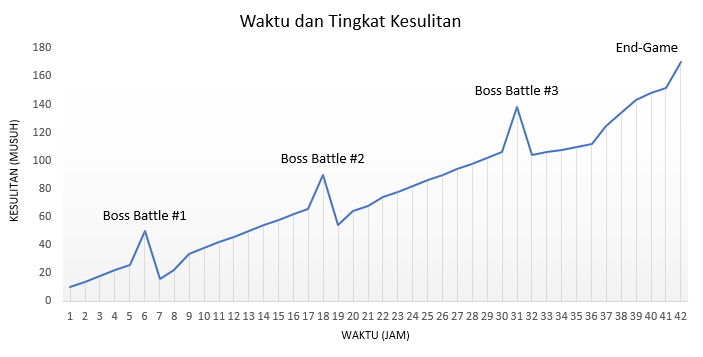
\includegraphics[scale=0.68]{img/story_dungeon.png}
			\caption{Pengaruh cerita terhadap tingkat kesulitan.}
			\label{fig:story_dungeon}
		\end{figure}
		
		Adapun beberapa cara untuk meminimalisir \textit{grinding} dan lamanya waktu permainan, dengan diberikan Exp (\textit{Experience} adalah sebuah variabel untuk pemain agar naik level) kepada pemain untuk menyelesaikan misi dan mengalahkan musuh yang lebih sulit dari pada mengalahkan musuh yang relatif mudah ditaklukan yang tersebar pada peta. Tentu saja musuh yang tersebar di peta juga memberikan Exp bagi pemain, namun seiring bertambahnya level pemain maka Exp yang diperoleh saat melawan musuh dengan level rendah akan semakin kecil.
		\vspace{1ex}
		
		Pada penelitian ini tingkat kesulitan langsung disimulasikan dengan pertarungan antara karakter-karakter yang dimainkan oleh pemain melawan musuh, dengan kondisi tingkat kesulitan musuh yang terus naik lalu turun kemudian naik lagi dan turun lagi, naik lagi dan seterusnya sampai dengan kondisi puncak. Hal ini mensimulasikan kondisi yang dilalui oleh pemain saat melawan \textit{trash mobs}, memasuki \textit{dungeon}, saat bertarung melawan bos dan kemudian pada akhirnya bertarung melawan bos terakhir. Lebih detailnya akan dijelaskan pada poin selanjutnya.
		\vspace{1ex}
	
		\item \textbf{Waktu yang Diperlukan untuk Kalahkan Musuh}
	
		Musuh pada permainan \textit{turn-based} RPG umumnya terbagi menjadi empat kategori diantaranya adalah:
		
		\begin{enumerate}[label=\Alph*).]
			\item \textit{Trash Mobs} adalah musuh yang tersebar pada seluruh area atau map.
			\item \textit{Dungeon Mobs} dapat dibagi menjadi dua sub-kategori:
			\begin{enumerate}[label=\alph*).]
				\item \textit{Dungeon Trash} atau sama seperti \textit{Trash Mobs} yang sebagian besar ditemukan awal sampai tengah \textit{dungeon}.
				\item \textit{Difficult Dungeon Trash} atau yang lebih sulit terletak lebih dekat ke bos atau dari tengah ke akhir \textit{dungeon}.
			\end{enumerate}
			\item \textit{Mini-Boss}/\textit{Boss Mobs}.
			\item \textit{End-Game Boss}/\textit{Secret Boss} (Bos yang bersifat opsional).
		\end{enumerate}
		
		Pada penelitian ini keseimbangan permainan dirancang terus meningkat seperti yang dibahas pada bagian sebelumnya, dalam permainan ini sebagian besar waktu (asumsikan saja 80\%) akan dihabiskan bertarung di dalam \textit{dungeon}. Kemudian 20\% dari waktu pertempuran akan digunakan untuk bertarung melawan bos. Sedangkan sisanya 60\% dari waktu bertarung akan dibagi antara pertarungan melawan musuh yang lemah dan juga kuat, bila digambarkan pembagian tersebut akan seperti pada Gambar \ref{fig:enemy_difficulty_percentage}.
		
		\begin{figure} [!h] \centering
			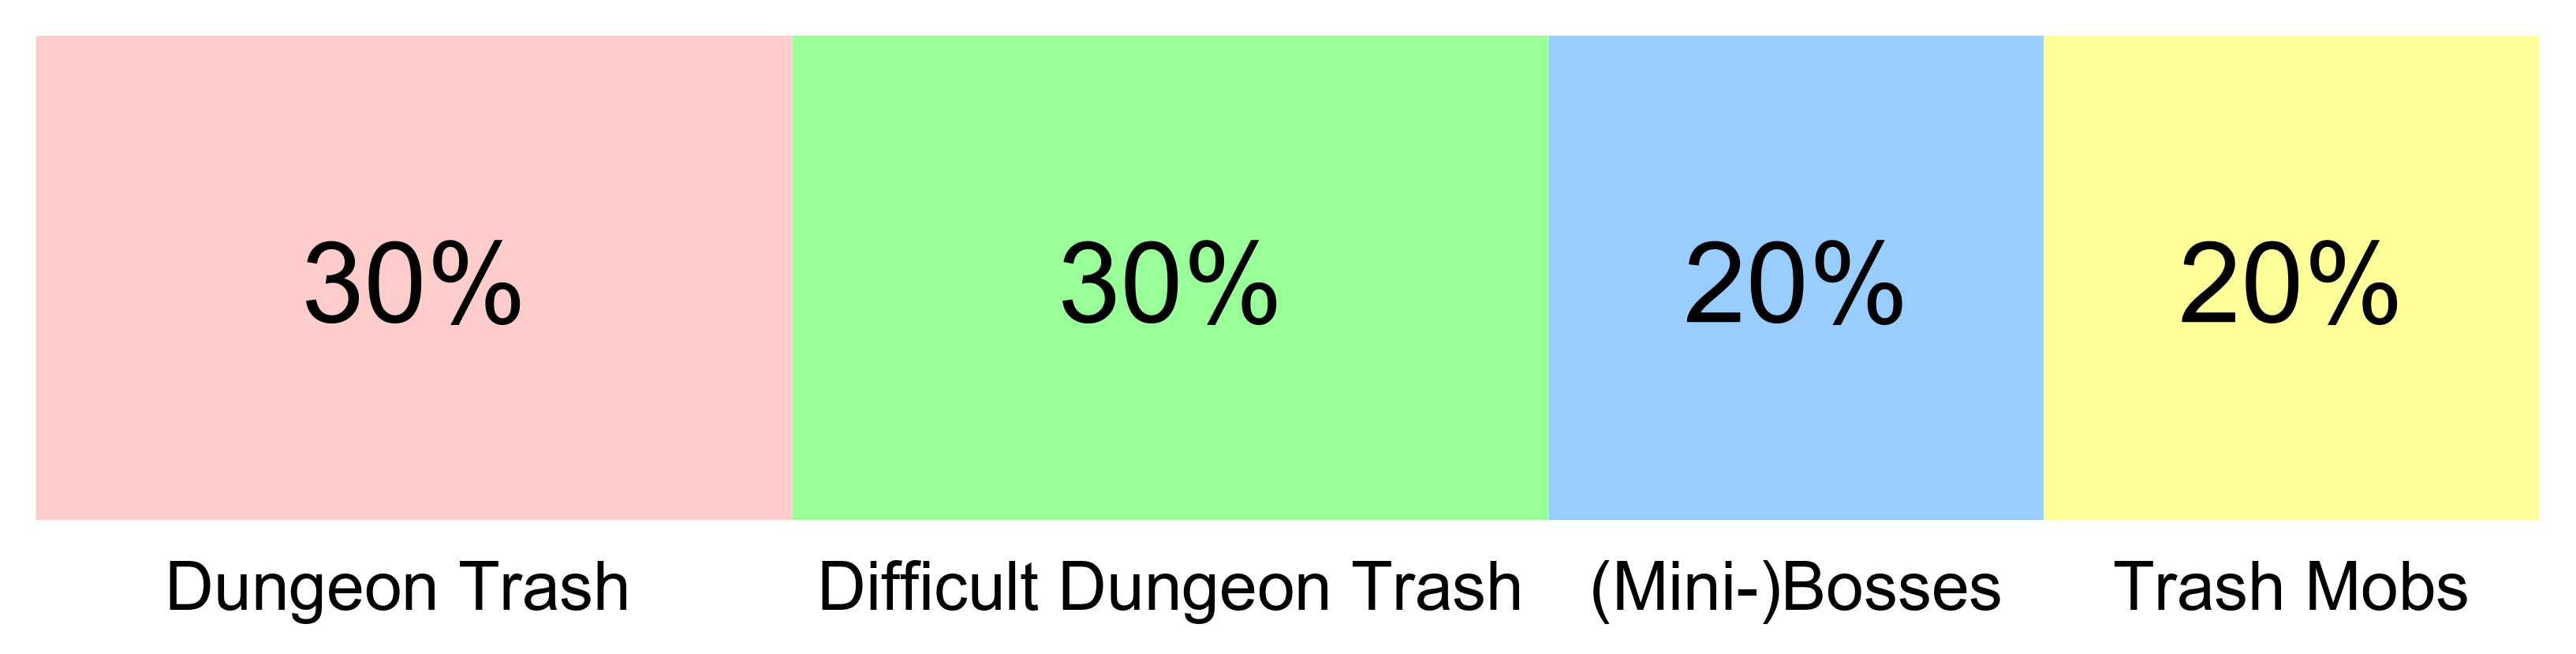
\includegraphics[scale=0.12]{img/enemy_type_distribution.png}
			\caption{Distribusi jenis musuh sesuai dengan cerita.}
			\label{fig:enemy_difficulty_percentage}
		\end{figure}
		
		Perhatikan bahwa dalam distribusi yang dibuat, jumlah waktu yang dihabiskan untuk melawan bos sama seperti waktu yang dibutuhkan untuk memerangi \textit{Thrash Mobs}. Dalam proses replikasi distribusi dalam permainan, pertama tentukan jumlah total waktu yang dibutuhkan oleh pemain untuk mengalahkan naga, raksasa atau apa pun yang biasanya disebut dengan bos.
		\vspace{1ex}
		
		Misalnya, dalam permaian RPG, bos pertama idealnya akan membutuhkan 3 menit bagi pemain yang kompeten untuk mengalahkan, dan bos terakhir menghabiskan waktu 20 menit. Kemudian terjadi peningkatan kompleksitas pada bos di level menengah, untuk terdapat dua bos yang masing-masing membutuhkan waktu sekitar 10 menit untuk dikalahkan, dan bos kedua membutuhkan waktu 7 menit.
		\vspace{1ex}
		
		\begin{equation}
		\label{eq: total_fight}
		B_{total} = \sum_{n = 0}^{k} B_{n}
		\end{equation}
		
		Merujuk ke persamaan \ref{eq: total_fight} bila dijabarkan maka $B_{total}$ adalah jumlah waktu melawan bos secara keseluruhan, jumlah bos dinyatakan dengan $k$ dan waktu yang dihabiskan untuk melawan satu bos dinyatakan dengan $B$ kemudian diiterasi oleh $n$ sejumlah $k$.
		\vspace{1ex}
		
		Di perlukannya penyesuaian terhadap model distribusi, salah satunya waktu yang habis untuk melawan bos setara untuk melawan musuh yang mudah atau \textit{trash mobs}. Untung saja terdapat banyak cara untuk memodifikasi waktu yang akan dihabiskan saat bertarung melawan musuh yang mudah. Hal seperti menjelajah seluruh peta atau berpetualang menuju tempat-tempat sebelumnya juga tidak perlu dilakukan. Berikut adalah langkah-langkah yang dapat dilakukan:
	
		\begin{enumerate} [label=\alph*).]
			\item  Mengurangi atau meningkatkan tingkat pertemuan dengan musuh yang mucul secara acak atau yang biasa disebut dengan \textit{random encounter rate}. Bisa juga dengan tingkat \textit{spawn} (muncul lagi setelah mati).
			\item Menambah atau mengurangi jumlah musuh saat pertempuran.
			\item Membatasi kemampuan musuh yang menimbulkan efek status yang menyulitkan dan menghabiskan waktu seperti \textit{confused}, \textit{silence}, \textit{tired} dan lain-lain.
			\item Menambah atau mengurangi kekuatan musuh.
			\item Menambah atau mengurangi kekuatan dari \textit{party member}.
		\end{enumerate}
	\end{enumerate}
\end{subs}

Terdapat banyak fleksibilitas di sini, developer dapat mengisi daftar musuh yang akan muncul secara acak dengan musuh yang sulit dikalahkan dengan tingkat probabilitas kemunculan yang kecil, atau lebih sering memunculkan musuh yang mudah dikalahkan. Alternatif lain adalah dengan meningkatkan kekuatan \textit{party member} atau jumlah rata-rata musuh yang bertarung dalam satu kali pertarungan. Kebebasan desain semacam ini yang nantinya akan memudahkan penyeimbangan permainan. Sedangkan jumlah musuh dan panjangnya level dari pemain atau musuh sendiri menggambarkan akan lamanya permainan tersebut. Pada dasarnya semua proses diatas mengacu pada pokok pembahasan dari referensi yang dibahas pada Sub-bab \ref{sec:sub_sec2_keseimbangan} tentang menemukan keseimbangan.
\vspace{1ex}

\section{Desain Level dan Stats pada Karakter Pemain}
\label{sec:sec3_player_stats}
\vspace{1ex}

Di buatlah sebuah program yang secara otomatis dapat membuat \textit{stats} dari pemain dengan masukan sesuai dengan kebutuhan desainer permainan atau developer. Program tersebut terdiri dari beberapa fungsi yang pada awalnya adalah obyek yang memiliki masukan parameter-parameter yang nantinya akan menghasilkan sebuah data yang berupa \textit{stats} dari karakter pemain seperti proses yang ditunjukan oleh diagram alur pada Gambar \ref{fig:player_stats_generator}.
\vspace{1ex}

\begin{figure} [!h] \centering
	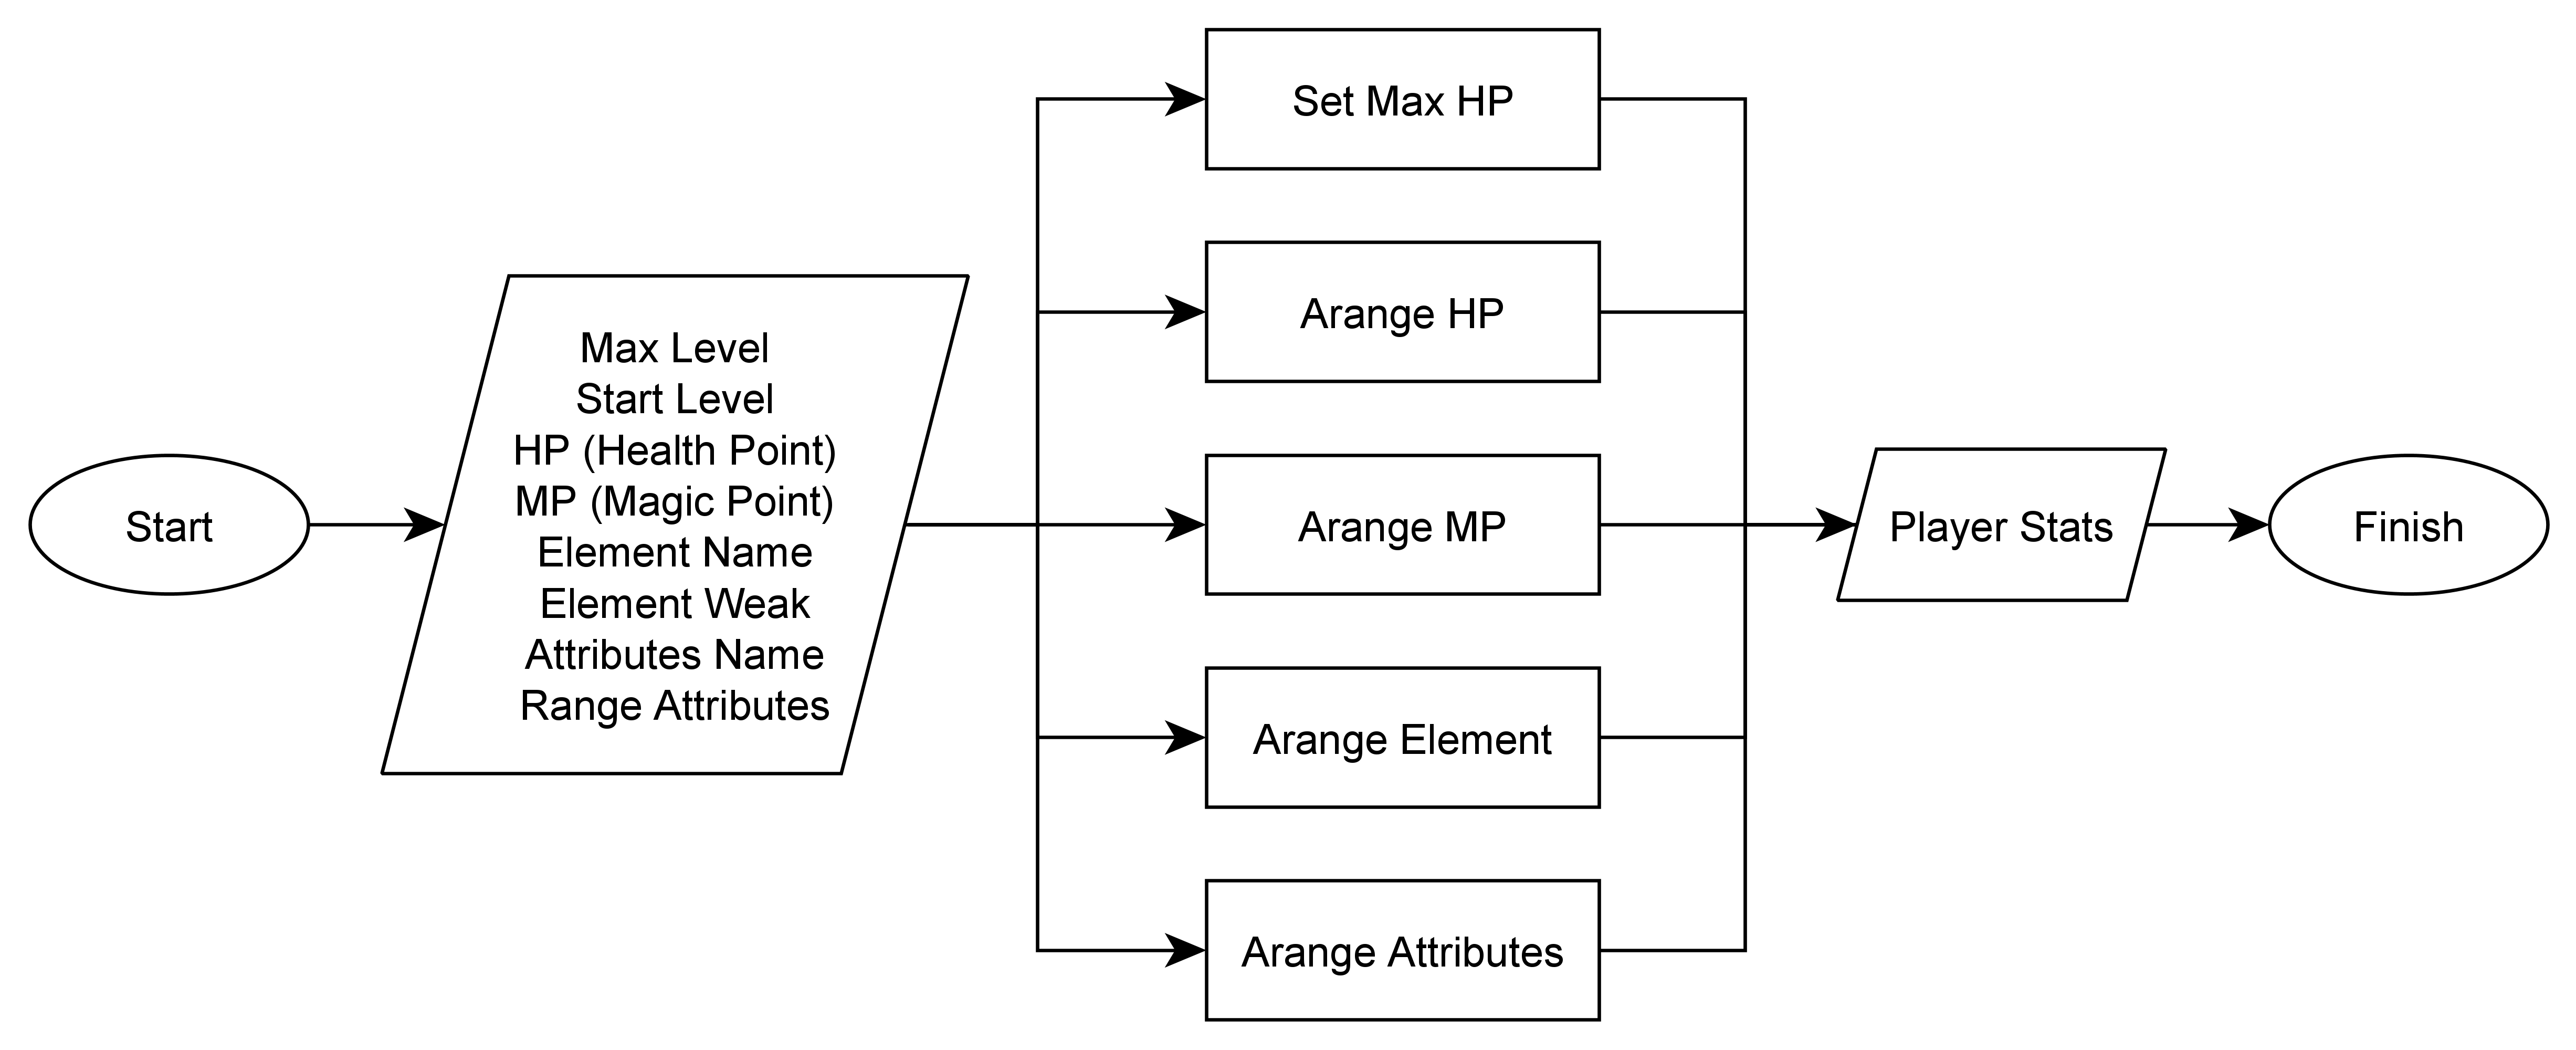
\includegraphics[scale=0.037]{img/player_stats_generator.png}
	\caption{Proses pembuatan stats untuk karakter pemain.}
	\label{fig:player_stats_generator}
\end{figure}

Pada permainan dengan genre \textit{turn-based} RPG dengan jumlah karakter yang dapat dimainkan berjumlah lebih dari satu, maka program yang ditunjukan melalui proses pada Gambar \ref{fig:player_stats_generator} akan dijalankan lebih dari satu kali. Hal tersebut dilakukan dengan tujuan agar karakter utama atau yang dapat dimainkan oleh pemain berjumlah lebih dari satu. Lain halnya dengan \textit{action} RPG, cukup hanya dengan satu kali menjalankan program maka sudah diperolehnya \textit{stats} dari karakter yang dibuat. Hal tersebut dikarenakan biasanya permainan dengan genre action RPG, jumlah karakternya hanya satu.
\vspace{1ex}

Pada Gambar \ref{fig:player_stats_generator} disisi masukan program terdapat banyak sekali masukan variabel seperti \textit{Max Level} yang berupa maksimum level yang di inginkan, kemudian \textit{Start Level} yang berupa level awal dari pemain, kemudian HP yang berupa \textit{range} atau jarak antara HP terendah dengan HP terendah setelah itu. Sama halnya dengan HP, dalam perhitungan \textit{range} atau jarak pada \textit{MP} juga menggunakan cara tersebut. Kemudian \textit{Element Name} berisi daftar elemen apa saja yang ingin digunakan, begitu juga dengan \textit{Name Stats}. Kemudian untuk \textit{Range Stats} berisikan \textit{stats} awal atau inisialisasi dan maksimum \textit{stats}. Lebih detail tentang program yang dibuat dapat dilihat pada Gambar \ref{fig:player_uml}, yang merupakan \textit{class} diagram untuk membuat \textit{stats} pemain.
\vspace{1ex}

\begin{figure} [!h] \centering
	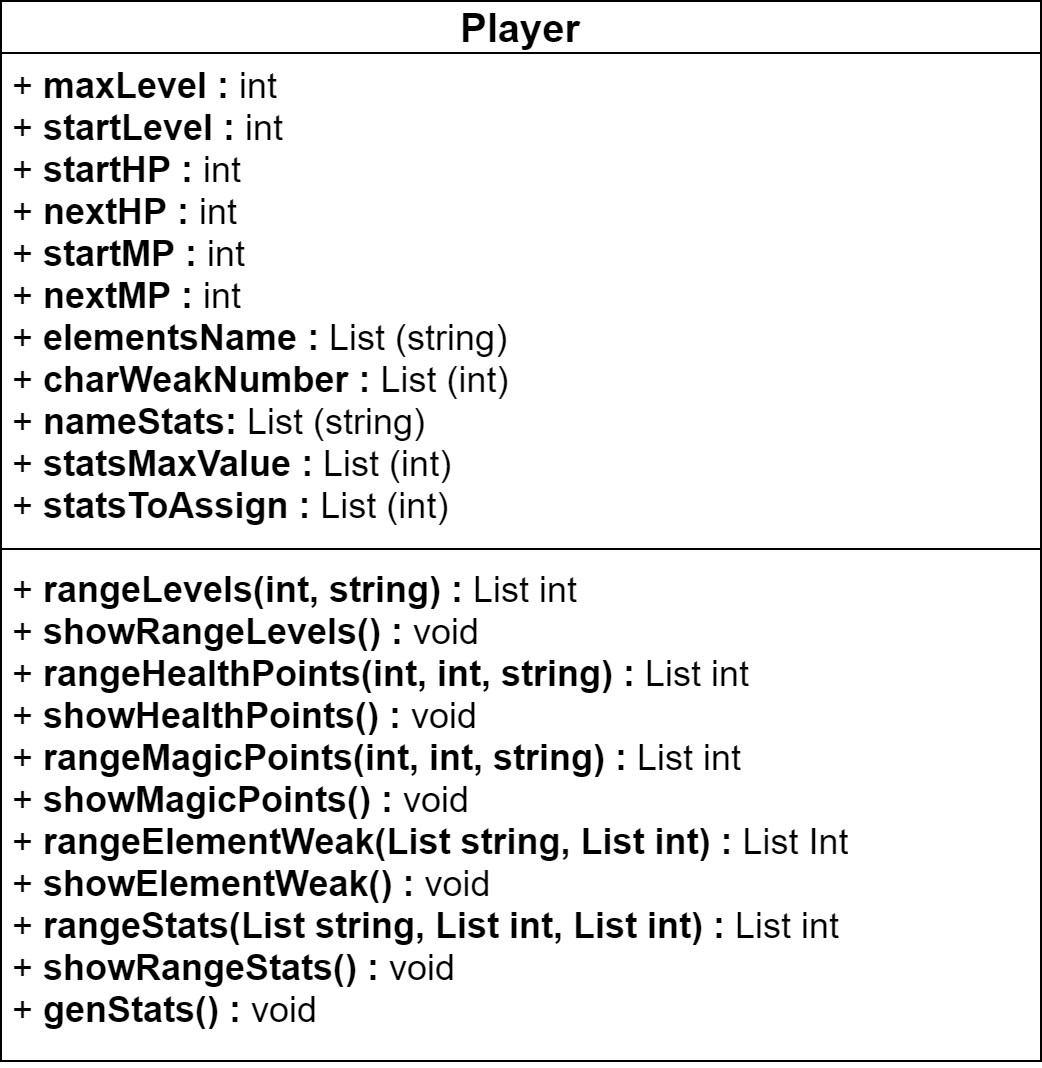
\includegraphics[scale=0.25]{img/player_uml.png}
	\caption{\textit{Class} diagram untuk \textit{stats} pemain.}
	\label{fig:player_uml}
\end{figure}

Karena program ini dibangun menggunakan OOP (\textit{Object Oriented Programming}) maka program ini dapat dijabarkan menggunakan Gambar \ref{fig:player_uml}. Selain itu program ini juga dapat secara mudah dimodifikasi untuk keperluan pengembangan kedepannya, dengan fungsi-fungsi yang ada sangat memungkinkan dilakukan \textit{override} atau pembuatan fungsi yang sama dengan isi atau proses yang berbeda.
\vspace{1ex}

Dalam menjelaskan proses pada BAB ini maka diambilah sebuah kasus dalam desain permainan, khususnya dalam penyusunan \textit{stats} untuk pemain dengan genre permaian \textit{turn-based} dan \textit{action} RPG. Pada Tabel \ref{tb:player_input_variable} adalah masukan untuk menguji program yang akan dijelaskan pada bagian selanjutnya, yang mana masukan pada Tabel \ref{tb:player_input_variable} akan menghasilkan \textit{stats} pada sebuah karakter untuk pemain.
\vspace{1ex}

\begin{table}[!h]
	\centering
	\caption{Data masukan untuk pembuatan \textit{stats} pemain.}
	\label{tb:player_input_variable}
	\begin{tabular}{|l|l|}
		\hline
		\rowcolor[HTML]{9B9B9B} 
		\multicolumn{1}{|c|}{\cellcolor[HTML]{9B9B9B}\textbf{Variabel}} & \multicolumn{1}{c|}{\cellcolor[HTML]{9B9B9B}\textbf{Input}} \\ \hline
		\textit{Max} Level & 100 \\ \hline
		\textit{Start} Level & 1 \\ \hline
		\textit{Start} HP & 159 \\ \hline
		\textit{Next} HP & 163 \\ \hline
		\textit{Start} MP & 89 \\ \hline
		\textit{Next} MP & 93 \\ \hline
		\textit{List Element} & {[} `Phys', `Water', `Wind', `Earth', `Fire' {]} \\ \hline
		\textit{List Weaknesess} & {[} 1, 2, 1, 1, 0 {]} \\ \hline
		\textit{List Stats Name} & {[} `Strength', `Magic', `Endurance', `Speed', `Luck' {]} \\ \hline
		\textit{Max Stats Value} & {[} 74, 38, 63, 65, 60 {]} \\ \hline
		\textit{Stats to Assign} & {[} 2, 1 {]} \\ \hline
	\end{tabular}
\end{table}
\vspace{1ex}

\subsection{Distribusi Level, HP dan MP Pemain}
\label{sec:sub_sec3_player_level_hp_mp}
\vspace{1ex}

Berdasarkan Tabel \ref{tb:player_input_variable} level untuk karakter pemain dimulai dari 1 dan level maksimalnya adalah 100, pada program ini level pemain akan terus naik satu demi satu level sampai ke tingkat maksimal. Selanjutnya adalah HP atau \textit{Health Point} yang diberi masukan berupa \textit{start} HP, bisa dinyatakan juga sebagai HP saat level satu. Kemudian variabel lanjutannya adalah \textit{next} HP atau HP pada level selanjutnya, misalkan level dua. Muncul sebuah pertanyaan berapa HP selanjutnya sampai dengan level ke 100. 
\vspace{1ex}

Cara semacam itu juga berlaku untuk perhitungan MP pada programm ini, dengan pola masukan yang sama dengan HP yaitu \textit{Start} MP dan \textit{Next} MP. Pada persamaan \ref{eq:hp_player} dan \ref{eq:mp_player} adalah contoh persamaan yang digunakan untuk mencari nilai HP dan MP selanjutnya.
\vspace{1ex}

\begin{equation}\label{eq:hp_player}
	\begin{split}
		HP(N) = \sum_{n = 0}^{N} HP(n + 1) + \left(HP(n + 1) - HP(n) \right)
	\end{split}
\end{equation}

\begin{equation}\label{eq:mp_player}
	\begin{split}
		MP(N) = \sum_{n = 0}^{N} MP(n + 1) + \left(MP(n + 1) - MP(n) \right)
	\end{split}
\end{equation}
\vspace{1ex}

Pada persamaan \ref{eq:hp_player} dan persamaan \ref{eq:mp_player} HP tetap dinyatakan sebagain HP, begitu juga dengan MP. Kemudian $HP(N)$ adalah nilai HP yang dicari, yang mana $N$ adalah level maksimum, $n$ adalah level mulai dan $n + 1$ adalah level selanjutnya. Jadi pada tahap ini seperti yang dijelaska pada Tabel \ref{tb:player_input_variable} yang mana nilai $n$ dan $n + 1$ sudah diketahui sebagai inisialisasi, masing-masing adalah $HP(n)$ dan $HP(n + 1)$. Penjelasan ini juga berlaku untuk mencari nilai $MP(N)$ yaitu nilai MP yang dicari. Hasil contoh perhitungan dari persamaan \ref{eq:hp_player} dan \ref{eq:mp_player} dengan masukan dari Tabel \ref{tb:player_input_variable} dapat hasilnya dapat dilihat pada Tabel \ref{tb:player_hp_mp}. 
\vspace{1ex}

\begin{table}[h!]
	\centering
	\caption{Hasil Perhitungan HP dan MP}
	\label{tb:player_hp_mp}
	\begin{tabular}{|l|l|l|}
		\hline
		\rowcolor[HTML]{C0C0C0} 
		\textbf{Levels} & \textbf{HP} & \textbf{MP} \\ \hline
		1 & 159 & 89 \\ \hline
		2 & 163 & 93 \\ \hline
		3 & 167 & 97 \\ \hline
		4 & 171 & 101 \\ \hline
		5 & 175 & 105 \\ \hline
		6 & 179 & 109 \\ \hline
		7 & 183 & 113 \\ \hline
		8 & 187 & 117 \\ \hline
		... & ... & ... \\ \hline
		\textbf{100} & \textbf{555} & \textbf{485} \\ \hline
	\end{tabular}
\end{table}
\vspace{1ex}

Hasil perhitungan tersebut terlihat membentuk pola linier, yang mana nilai HP dan MP terus naik secara konstan ke atas sesuai dengan kenaikan levelnya seperti yang direpresentasikan pada Gambar \ref{fig:hp_player} dan Gambar \ref{fig:mp_player}.

\begin{figure} [!h] \centering
	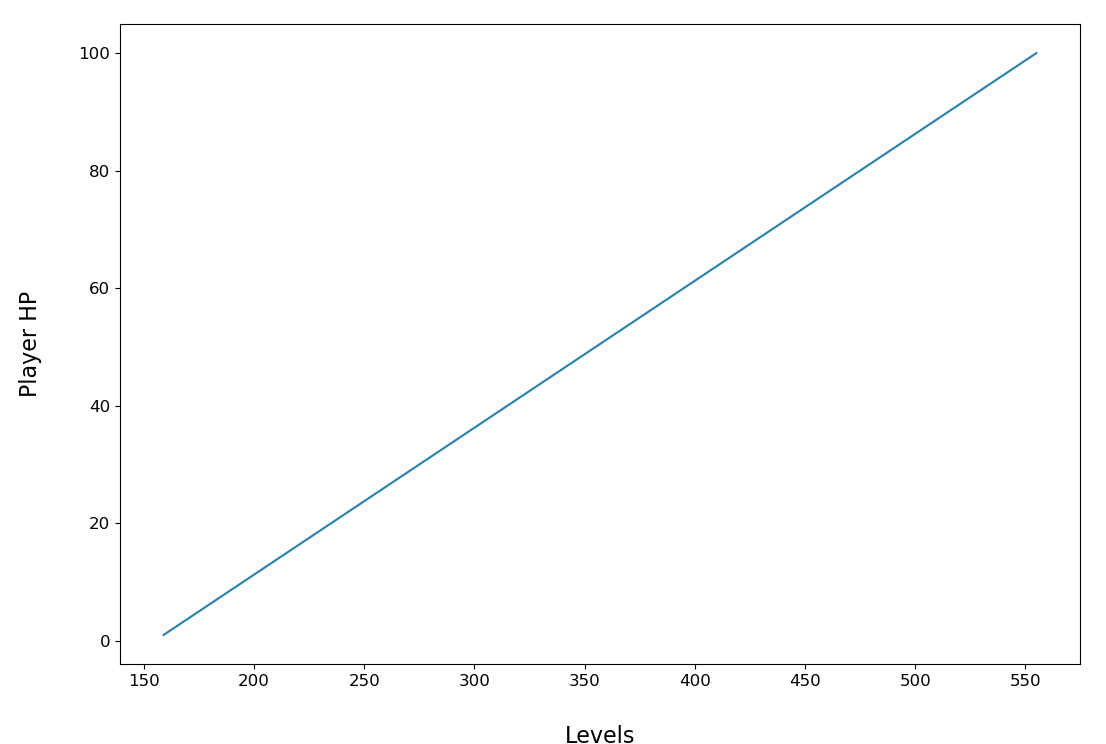
\includegraphics[scale=0.5]{img/PlayerHpDistrib.png}
	\caption{Kenaikan HP setiap levelnya.}
	\vspace{1ex}
	\label{fig:hp_player}
\end{figure}
\vspace{3ex}

\begin{figure} [!h] \centering
	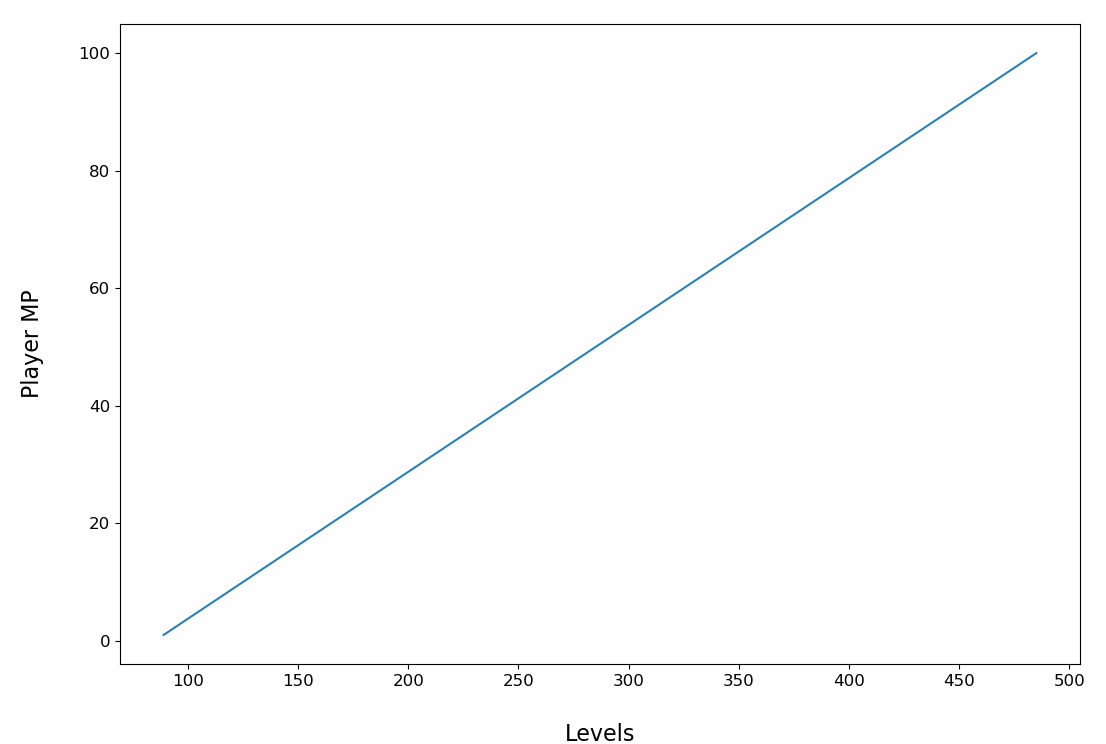
\includegraphics[scale=0.5]{img/PlayerMpDistrib.png}
	\caption{Kenaikan MP setiap levelnya.}
	\label{fig:mp_player}
\end{figure}

Jika melihat Gambar \ref{fig:hp_player} dengan jumlah HP dari pemain yang terus naik mengikuti pola yang dihasilkan pada Tabel \ref{tb:player_hp_mp}, yang mana nilai tersebut diperoleh dari inisiasi variabel pada Tabel \ref{tb:player_input_variable} yaitu \textit{Max Level}, \textit{Start} HP dan \textit{Next} HP. Variabel-variabel tersebut dihitung dengan menggunakan persamaan \ref{eq:hp_player} agar membentuk pola kenaikan HP setiap levelnya seperti yang ditunjukan pada Gambar \ref{fig:hp_player}.
\vspace{1ex}

Sama seperti pada Gambar \ref{fig:hp_player}, pada Gambar \ref{fig:mp_player} dengan jumlah MP dari pemain yang terus naik mengikuti pola yang dihasilkan pada Tabel \ref{tb:player_hp_mp}, yang mana nilai tersebut diperoleh dari inisiasi variabel pada Tabel \ref{tb:player_input_variable} yaitu \textit{Max Level}, \textit{Start} MP dan \textit{Next} MP. Kemudian variabel-variabel tersebut dihitung dengan menggunakan persamaan \ref{eq:mp_player} agar membentuk pola kenaikan MP setiap levelnya seperti yang ditunjukan pada Gambar \ref{fig:mp_player}.
\vspace{1ex}

\subsection{Distribusi Elemen dan Kelemahan Pemain}
\label{sec:sub_sec3_list_element_player}
\vspace{1ex}

Kemudian untuk variabel \textit{List Element} berisi elemen apa saja yang akan diterapkan pada permainan tersebut, seperti yang ditunjukan oleh Tabel \ref{tb:player_input_variable}. Yang mana maksud dari variabel ini adalah memberi penjelasan dari kelemahan dan keunggulan dari pemain berdasarkan elemen, seperti yang sudah dijelasakan pada Sub-bab \ref{sec:sub_sec3_design_skenario} tentang elemen dan efektifitas serangan. Di lanjutkan dengan variabel \textit{List Weaknesses} yang memuat angka-angka yang bertujuan menggambarkan saat pemain menerima serangan dari lawan, berikut adalah penjelasan dari angka-angka tersebut.

\begin{enumerate}[label=\alph*).]
	\item \textbf{Angka 0} adalah \textit{Normal} atau efek serangan bersifat normal tanpa tambahan bonus serangan dan lain sebagainya.
	
	\item \textbf{Angka 1} adalah \textit{Repel} atau memiliki sifat menghindari serangan atau bahkan menghindari serangan.
	
	\item \textbf{Angka 2} adalah \textit{Weaknesess} atau serangan tepat menyerang terhadap kelemahan dari pemain sehingga efek kerusakan atau \textit{damage} menjadi lebih terasa, biasanya dua kali serangan normal.
\end{enumerate}

Pembagian elemen pada pemain bersifat pada penelitian ini dibuat statis, maksudnya elemen yang dari awal didefinisikan tidak akan berubah sampai akhir level, untuk kedepannya hal seperti inilah yang akan menjadi konsetrasi pengembangan program ini berikut juga desainer permainan. Cukup dengan melakukan \textit{override} maka diperolehlah fungsi baru yang bisa menghasilkan perubahan elemen di level tertentu.
\vspace{1ex}

Pada bagian selanjutnya adalah pembahasan mengenai pembagian \textit{stats} jika merujuk pada Tabel \ref{tb:player_input_variable} dengan variabel \textit{List Stats Name} yang berisi nama atau info \textit{stats} dari pemain yang akan digunakan. Kemudian diikuti dengan variabel \textit{Max Stats Value} yang berisi nilai maksimum \textit{stats} yang akan dihasilkan. Lebih detailnya untuk bagian ini, akan dibahas secara khusus pada bagian tersendiri yaitu pada Sub-bab \ref{sec:sub_sec3_stat_pemain}.
\vspace{1ex}

\subsection{Distribusi Stats Pemain}
\label{sec:sub_sec3_stat_pemain}
\vspace{1ex}

Pada bagian ini akan dibahas tentang pembagian \textit{stats} dengan beracuan pada Tabel \ref{tb:player_input_variable} dengan variabel \textit{List Stats Name} yang berisi nama atau info \textit{stats} dari pemain yang akan digunakan. Kemudian diikuti dengan variabel \textit{Max Stats Value} yang berisi nilai maksimum \textit{stats} yang akan dihasilkan. Pada tahap ini digunakannya metode $k-$Nearest Neighbor ($k-$NN) seperti yang sudah dijelaskan pada Sub-bab \ref{sec:sub_sec2_knn} dan Naive Bayes yang juga sudah dijelaskan pada Sub-bab \ref{sec:sub_sec2_bayes}. Pada persamaan \ref{eq:KNN_distance_metrics} yang kemudian disesuaikan dengan pertambahan nilai \textit{Stats to Assign} dari Tabel \ref{tb:player_input_variable}, yang mana nilai tersebut ditambahkan secara acak antara 2 dan 1 dengan perhitungan \textit{class probability} pada persamaan \ref{eq:nbayes_class} yang disesuaikan menjadi persamaan \ref{eq:nbayes_class_stats}. Hasil proses acak tersebut juga harus dibatasi jumlahnya dengan persamaan \ref{eq:KNN_distance_stats}. Maka hasil dari proses acak pada persamaan tersebut akan sangat menentukan perhitungan dari persamaan \ref{eq:KNN_bayes_player_stats}.

\begin{equation}\label{eq:nbayes_class_stats}
\begin{split}
P(C_{St = 1}) = \frac{C_{St = 1}}{(C_{St = 1}\ +\ C_{St = 2})} \\
P(C_{St = 2}) = \frac{C_{St = 2}}{(C_{St = 1}\ +\ C_{St = 2})}
\end{split}
\end{equation}

\begin{equation}\label{eq:KNN_distance_stats}
\begin{split}
D(x,\ p) = \sqrt{(x - p)^2}
\end{split}
\end{equation}

\begin{equation}\label{eq:KNN_bayes_player_stats}
\begin{split}
MaxSt = \left\{\begin{matrix}
\sum_{n = 0}^{N}\ St_{(n)}, & saat\ D(x,\ p) \geqslant 2,\ St = 2 \\ 
\sum_{n = 0}^{N}\ St_{(n)}, & saat\ D(x,\ p) \geqslant 1,\ St = 1 \\
\hspace{4.5em} 0, 			& \hspace{-7.8em} lainnya
\end{matrix}\right.
\end{split}
\end{equation}

Pada persamaan \ref{eq:nbayes_class}, variabel $P(C_{St = 1})$ adalah probabilitas munculnya \textit{Stats To Assign} ke 1 dan $P(C_{St = 2})$ adalah probabilitas munculnya \textit{Stats To Assign} ke 2, kemudian $C_{St = 1}$ adalah jumlah angka satu dan $C_{St = 2}$ adalah jumlah angka satu pada \textit{Stats To Assign}. Setiap stats hasil pengacakan tentunya juga akan dibatasi jumlahnya dengan melakukan \textit{checking} pada maksimum stats, hal tersebut dijelaskan pada persamaan \ref{eq:KNN_distance_stats} yang mana $x$ adalah maksimum stats, $D$ adalah maksimum stats dan $p$ adalah stats saat ini. Kemudian nilai $MaxSt$ pada persamaan \ref{eq:KNN_bayes_player_stats} adalah nilai maksimum stats yang ingin dicapai dengan jumlah $St_{(n)}$ yang dihitung melalui proses pada persamaan \ref{eq:KNN_distance_stats} dan \ref{eq:nbayes_class_stats}.

\begin{equation}\label{eq:nbayes_class_stats_1}
\begin{split}
P(C_{St = n}) = \frac{C_{St = n}}{(C_{St = 0}\ +\ C_{St = 1} +\ C_{St = n})}
\end{split}
\end{equation}

\begin{equation}\label{eq:KNN_distance_stats_1}
\begin{split}
D(x,\ p) = \sqrt{(x - p)^2}
\end{split}
\end{equation}

\begin{equation}\label{eq:KNN_bayes_player_stats_1}
\begin{split}
MaxSt = \left\{\begin{matrix}
\sum_{n = 0}^{N}\ St_{(n)}, & saat\ D(x,\ p) \geqslant n_{st},\ St = n_{st} \\
\sum_{n = 0}^{N}\ St_{(n)}, & \hspace{-1.5em}saat\ D(x,\ p) \geqslant 2,\ St = 2 \\
\sum_{n = 0}^{N}\ St_{(n)}, & \hspace{-1.5em}saat\ D(x,\ p) \geqslant 1,\ St = 1 \\
\hspace{4.5em} 0, 			& \hspace{-9.3em} lainnya
\end{matrix}\right.
\end{split}
\end{equation}

Sedangakan pada persamaan \ref{eq:nbayes_class_stats_1}, \ref{eq:KNN_distance_stats_1} dan \ref{eq:KNN_bayes_player_stats_1} digunakan saat jumlah atau dimensi \textit{Stats to Assign} lebih dari 2. Selanjutnya melalui persamaan \ref{eq:KNN_bayes_player_stats} dan beberapa persamaan yang digunakan sebelumnya dihasilkan data seperti yang ditunjukan pada Tabel \ref{tb:player_battle_stats}, dan bila divisualisasikan hasilnya akan tampak seperti pada Gambar \ref{fig:stats_player}.
\vspace{1ex}

\begin{table}[!h]
	\centering
	\caption{Sampel hasil perhitungan dan distribusi stats dengan $k-$NN}
	\label{tb:player_battle_stats}
	\begin{tabular}{|l|l|l|l|l|l|}
		\hline
		\rowcolor[HTML]{C0C0C0} 
		\textbf{Levels} & \textbf{Strength} & \textbf{Magic} & \textbf{Endurance} & \textbf{Speed} & \textbf{Luck} \\ \hline
		1 & 1 & 2 & 0 & 0 & 1 \\ \hline
		2 & 0 & 2 & 0 & 2 & 0 \\ \hline
		3 & 1 & 0 & 0 & 0 & 0 \\ \hline
		4 & 1 & 1 & 0 & 0 & 0 \\ \hline
		5 & 1 & 1 & 0 & 0 & 0 \\ \hline
		6 & 1 & 1 & 0 & 2 & 1 \\ \hline
		7 & 0 & 0 & 0 & 0 & 1 \\ \hline
		8 & 1 & 0 & 0 & 0 & 0 \\ \hline
		... & ... & ... & ... & ... & ... \\ \hline
		\textbf{100} & \textbf{1} & \textbf{0} & \textbf{0} & \textbf{0} & \textbf{0} \\ \hline
	\end{tabular}
\end{table}
\vspace{1ex}

Pada Tabel \ref{tb:player_battle_stats} adalah data \textit{stats} dari pemain yang dihasilakn melalui penambahan nilai pada \textit{stats} secara acak pada setiap \textit{stats}. Seperti yang dijelaskan pada persaamaan \ref{eq:nbayes_class}, \ref{eq:KNN_distance_stats}, dan persamaan \ref{eq:KNN_bayes_player_stats} saat nilai \textit{stats} di tambahkan secara acak dari 1 sampai dengan 2 pada level yang berjarak antara 1 sampai dengan 100. Selanjutnya representasi dari hasil penambahan \textit{stats} tersebut yang ditunjukan melalui Gambar \ref{fig:stats_player} yang mana nilai dari setiap \textit{stats} terus naik sesuai dengan level pemain yang juga terus naik. 
\vspace{1ex}

\begin{figure} [!h] \centering
	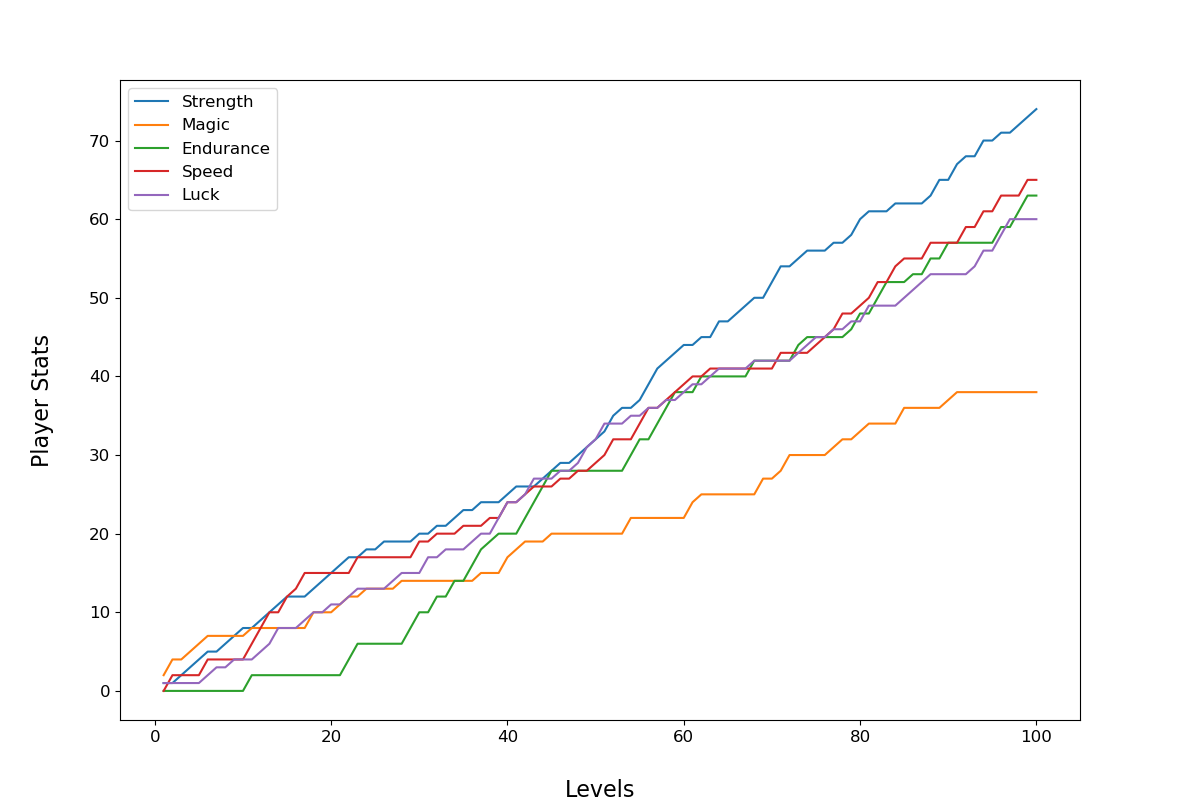
\includegraphics[scale=0.5]{img/PlayerStatsDistrib.png}
	\caption{Kenaikan stats pemain setiap levelnya.}
	\label{fig:stats_player}
\end{figure}
\vspace{1ex}

\section{Desain Level dan Stats pada Karakter Musuh}
\label{sec:sec3_enemy_stats}
\vspace{1ex}

Sama halnya dengan karakter pemain maka dibuatlah sebuah program yang secara otomatis dapat membuat \textit{stats} musuh dengan masukan sesuai dengan kebutuhan desainer permainan atau developer. Program tersebut terdiri dari beberapa fungsi yang pada awalnya adalah obyek yang memiliki masukan parameter-parameter yang nantinya akan menghasilkan sebuah data yang berupa \textit{stats} dari karakter pemain seperti proses yang ditunjukan oleh diagram alur sederhana pada Gambar \ref{fig:enemy_stats_generator}.
\vspace{1ex}

\begin{figure} [!h] \centering
	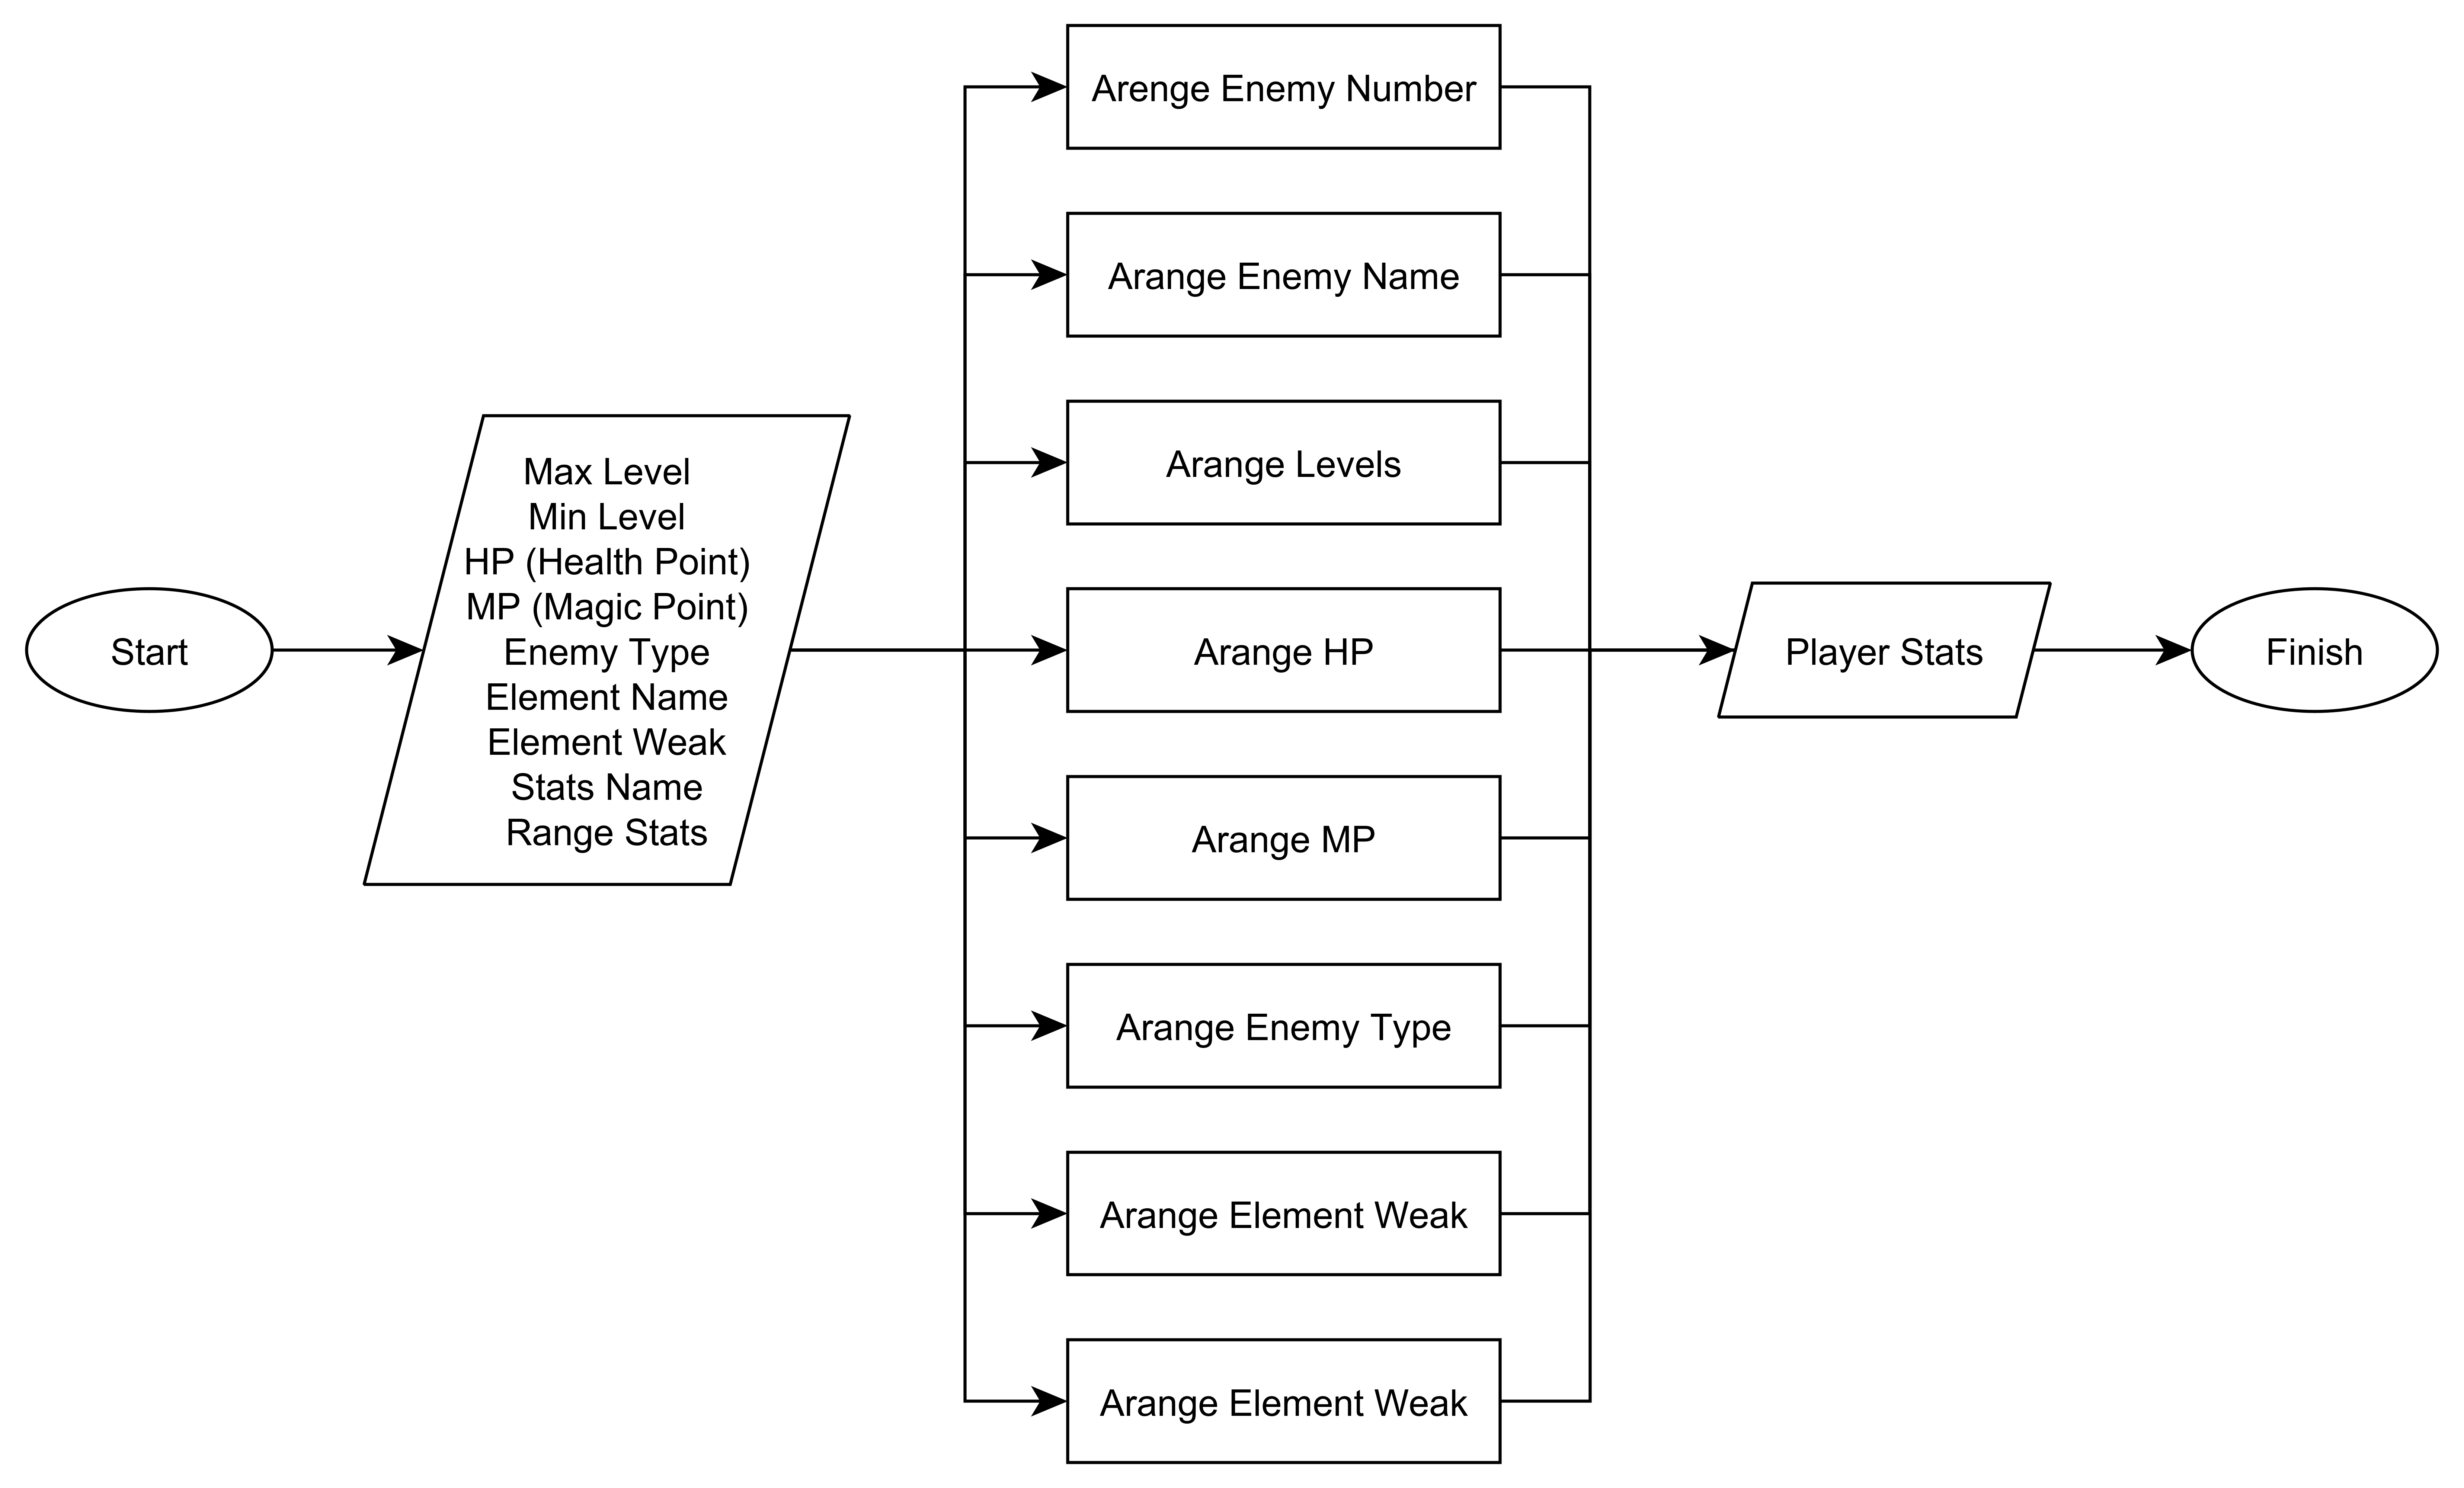
\includegraphics[scale=0.06]{img/enemy_stats_generator.png}
	\caption{Proses pembuatan stats untuk karakter musuh.}
	\label{fig:enemy_stats_generator}
\end{figure}

Pada permainan dengan genre \textit{turn-based} RPG dengan jumlah yang sangat banyak dan beragam, maka program yang ditunjukan melalui proses pada Gambar \ref{fig:enemy_stats_generator} dapat dijalankan satu kali saja, dan menghasilkan banyak musuh. Kecuali ingin menghasilkan kombinasi musuh yang berbeda, misalnya pada proses \textit{generate} yang pertama menghasilkan musuh yang memiliki kemampuan \textit{magic} dan kelemahan sedangkan pada kombinasi musuh selanjutnya tidak memiliki kemampuan \textit{magic}, hanya mengandalkan kemampuan fisik saja. Sama halnya dengan permainan \textit{action} RPG saat proses pembuatan stats musuh.
\vspace{1ex}

Pada Gambar \ref{fig:enemy_stats_generator} di sisi masukan program terdapat banyak sekali masukan variabel seperti \textit{Max Level} yang berupa maksimum level yang diinginkan, kemudian \textit{Min Level} yang berupa minimum level dari musuh, kemudian HP yang berupa \textit{range} atau jarak antara HP minimum dengan HP tertinggi. Sama halnya dengan HP, dalam perhitungan \textit{range} atau jarak, pada \textit{MP} juga menggunakan perhitungan dengan cara tersebut. Kemudian \textit{Enemy Type} yang berisi klasifikasi jenis stats musuh, tergolong musuh seperti apakah stats yang dihasilkan tersebut. Selanjutnya adalah \textit{Element Name} yang berisi daftar elemen apa saja yang dapat dipilih saat pembuatan karakter musuh, selanjutnya \textit{Element Weak} berisi tetang kelemahan dan keunggulan dari musuh tersebut ketika diserang, apakah saat diserang dengan menggunakan elemen tersebut akan mengalami kerusakan atau damage yang parah, normal atau tidak mempan sama sekali. Kemudian untuk \textit{Stats Name} berisikan nama \textit{stats} yang dipakai dalam membuat karakter musuh. Selanjutnya adalah isi atau data dari \textit{stats} itu sendiri yang menentukan karakter dari musuh itu sendiri, seberapa kuat musuh tersebut dalam menyerang atau bertahan dan lain sebagainya. Lebih detail tentang program yang dibuat dapat dilihat pada Gambar \ref{fig:enemy_uml}, yang merupakan \textit{class} diagram untuk membuat \textit{stats} pemain.
\vspace{1ex}

\begin{figure} [!h] \centering
	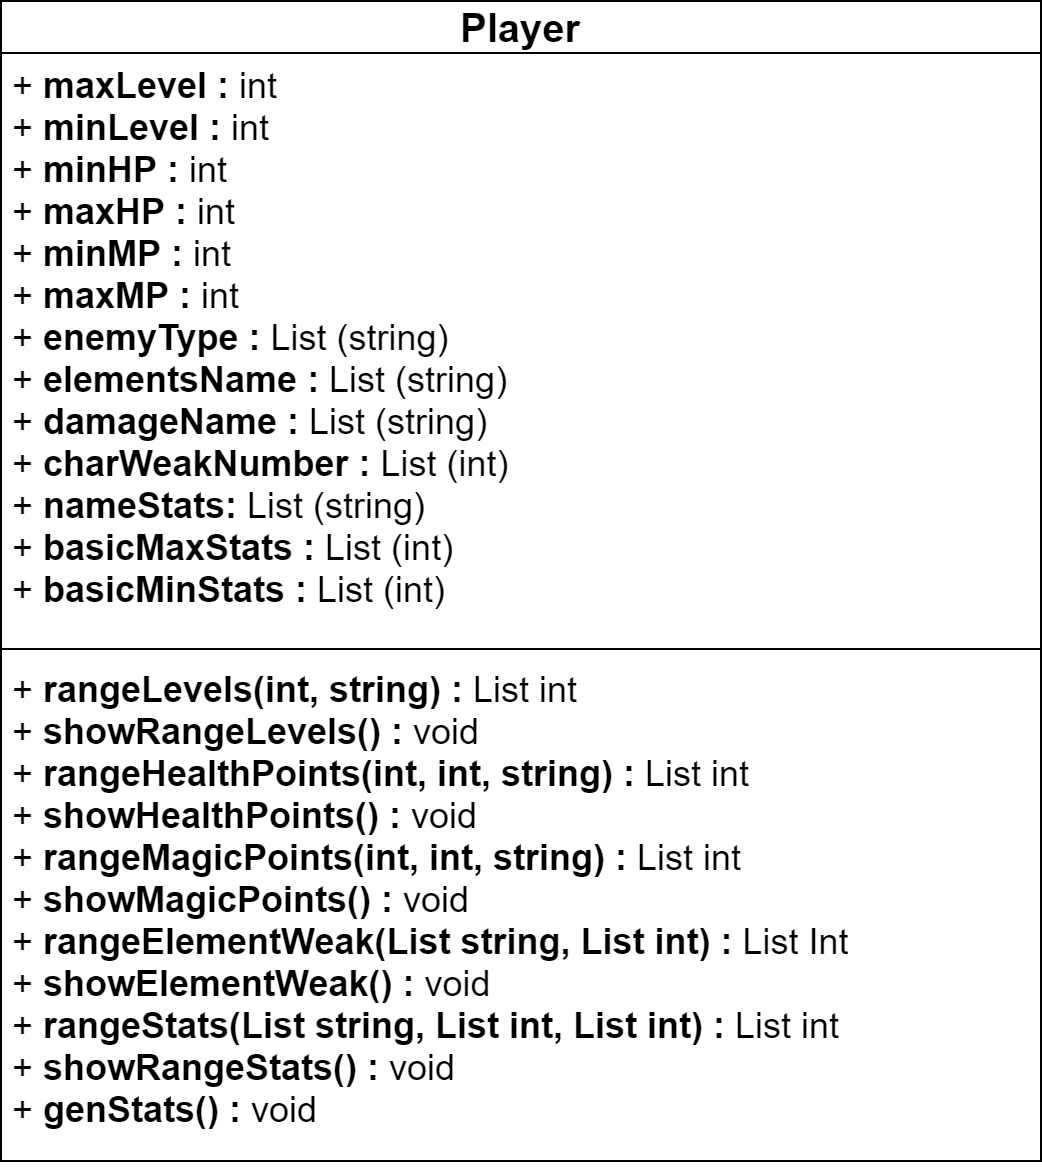
\includegraphics[scale=0.25]{img/enemy_uml.png}
	\caption{\textit{Class} diagram untuk \textit{stats} musuh.}
	\label{fig:enemy_uml}
	\vspace{-1ex}
\end{figure}

Karena program ini dibangun menggunakan OOP (\textit{Object Oriented Programming}) maka program ini dapat dijabarkan menggunakan Gambar \ref{fig:enemy_uml}. Selain itu program ini juga dapat secara mudah dimodifikasi untuk keperluan pengembangan kedepannya, dengan fungsi-fungsi yang ada sangat memungkinkan dilakukan \textit{override} atau pembuatan fungsi yang sama dengan isi atau proses yang berbeda seperti pada penjelasan dibagian pemain pada Sub-bab \ref{sec:sec3_player_stats}. Seperti pada bagian sebelumnya maka dibuatlah Tabel \ref{tb:enemy_input_variable} yang berupa masukan untuk menguji program yang akan dijelaskan pada bagian-bagian selanjutnya, yang mana masukan pada tabel tersebut akan menghasilkan stats pada sebuah karakter untuk pemain.
\vspace{1ex}

\begin{table}[!h]
	\centering
	\caption{Data masukan untuk pembuatan program pada musuh.}
	\label{tb:enemy_input_variable}
	\begin{tabular}{|l|l|}
		\hline
		\rowcolor[HTML]{9B9B9B} 
		\multicolumn{1}{|c|}{\cellcolor[HTML]{9B9B9B}\textbf{Variabel}} & \multicolumn{1}{c|}{\cellcolor[HTML]{9B9B9B}\textbf{Input}} \\ \hline
		\textit{Enemy Numbers} & 400 \\ \hline
		\textit{Max Level} & 80 \\ \hline
		\textit{Min Level} & 1 \\ \hline
		\textit{Level Class} & {[} `\textit{Easy}', `\textit{Medium}', `\textit{High}' {]} \\ \hline
		\textit{Min} HP & 159 \\ \hline
		\textit{Max} HP & 163 \\ \hline
		\textit{Min} MP & 89 \\ \hline
		\textit{Max} MP & 93 \\ \hline
		\textit{Enemy Type} & \begin{tabular}[c]{@{}l@{}}{[} `\textit{Mixed}', `\textit{Hard Magic}', `\textit{Soft Magic}', \\ \ \ `\textit{Hard Strength}', `\textit{Soft Magic}' {]}\end{tabular} \\ \hline
		\textit{Distribution Percentage} & {[} 40, 10, 20, 10, 20 {]} \\ \hline
		\textit{List Element} & {[} `\textit{Phys}', `\textit{Water}', `\textit{Wind}', `\textit{Earth}', `\textit{Fire}' {]} \\ \hline
		\textit{List Damage} & {[} `\textit{Normal}', `\textit{Repel}', `\textit{Weak}' {]} \\ \hline
		\textit{List Stats Name} & \begin{tabular}[c]{@{}l@{}}{[} `\textit{Strength}', `\textit{Magic}', `\textit{Endurance}',\\ \ \ `\textit{Speed}', `\textit{Luck}' {]}\end{tabular} \\ \hline
		\textit{Max Stats Value} & {[} 50, 60, 40, 55, 45 {]} \\ \hline
		\textit{Min Stats Value} & {[} 2, 2, 2, 2, 2 {]} \\ \hline
	\end{tabular}
\end{table}

\subsection{Distribusi Level Musuh}
\label{sec:sub_sec3_enemy_level}
\vspace{1ex}

Pada bagian ini akan dijelaskan tentang pembagian level pada musuh, dengan masukan seperti yang disebutkan pada Tabel \ref{tb:enemy_input_variable}. Beracuan pada tabel tersebut beberapa variabel utama yang akan digunakan diantaranya adalah ``\textit{Enemy Numbers}" yang menentukan jumlah musuh yang akan dibuat, ``\textit{Max Level}" dan ``\textit{Min Level}" adalah nilai maksimum dan minimum level dari musuh yang ingin dibuat. Selanjutnya tingkat kesulitan dari musuh juga ditentukan disini, dengan variabel ``\textit{Level Class}" yang isinya dibagi menjadi ``\textit{Easy}", ``\textit{Medium}" dan ``\textit{Hard}". Musuh dengan \textit{``Level Class"} atau tingkat kesulitan \textit{``Easy"} akan menjadi yang paling mudah dikalahkan, diikuti daengan tingkat kesulitan \textit{``Medium"} dan ``\textit{Hard}" secara berurutan.
\vspace{1ex}

Kemudian terdapat variabel pendukung yang akan menentukan data atau level yang ingin dihasilkan, yaitu \textit{scale}. Selaanjutnya dilakukan beberapa proses seperti pada persamaan \ref{eq:enemy_levels1}, \ref{eq:enemy_levels2}, \ref{eq:sub_enemy_levels1}, dan persamaan \ref{eq:sub_enemy_levels2} yang kemudian diperoleh hasil berupa level untuk banyak musuh sekaligus seperti yang ditunjukan pada persamaan \ref{eq:probability_enemy_levels}.
\vspace{1ex}

\begin{equation}\label{eq:enemy_levels1}
	\resizebox{\columnwidth}{!}{%
		$SL_{N} = \left\{\begin{matrix}
		\hspace{0.2em} \sum_{i = 0}^{N}\ \frac{LN}{LC_{N}} & Saat\ 0 \equiv LN\ (mod\ LC_{N}) & \\
		
		\hspace{0.2em} \sum_{i = 0}^{N}\ \frac{LN}{LC_{N}} & Saat\ 0 \not\equiv LN\ (mod\ LC_{N}), & \\
		&\hspace{1.0em}  0 \not\equiv LC_{N}\ (mod\ 2) & \hspace{-3.5em} \Rightarrow\ SL_{(\left \lceil N/2 \right \rceil)}  = \left \lceil \frac{LN}{LC_{N}} \right \rceil &\\
		
		& & \hspace{-6.0em} \Rightarrow\ SL_{i}  = \left \lfloor \frac{LN}{LC_{N}} \right \rfloor &\\
		
		\hspace{0.2em} \sum_{i = 0}^{N}\ \frac{LN}{LC_{N}} & Saat\ 0 \not\equiv LN\ (mod\ LC_{N}), & \\
		&\hspace{1.0em}  0 \equiv LC_{N}\ (mod\ 2) & \Rightarrow\ SL_{N/2},\ SL_{(N/2) + 1}  = \left \lceil \frac{LN}{LC_{N}} \right \rceil &\\
		
		& & \hspace{-6.0em} \Rightarrow\ SL_{i}  = \left \lfloor \frac{LN}{LC_{N}} \right \rfloor &\\
		\end{matrix}\right.$%
	}
\end{equation}
\vspace{1ex}

Pada persamaan \ref{eq:enemy_levels1} adalah proses pembagian dari jumlah level dari musuh yang dijelaskan pada Tabel \ref{tb:enemy_input_variable} pada variabel \textit{Max Level} dan \textit{Min Level} sebagai \textit{range} yang merupakan level dari musuh yang disimbolkan dengan $LN$ yang kemudian dibagi dengan  $LC_{N}$ yang merupakan jumlah kelompok atau \textit{cluster} data dari \textit{level class}. Jika beracuan pada Tabel \ref{tb:enemy_input_variable} maka jumlah \textit{cluster} level adalah jumlah data atau level yang dimuat pada setiap variabel didalam ``\textit{Level Class}" seperti ``\textit{Easy}", ``\textit{Medium}" dan ``\textit{High}", jadi jumlah levelnya adalah 3 \textit{cluster} level. Jadi pada kasus yang dicontohkan ini $LC = \left \{1, 2, 3 \right \}$, kemudian jika jumlah \textit{cluster} level ingin dibuat lebih dari contoh maka $LC = \left \{1, 2, 3,..., LC_{N} \right \}$ dengan $N$ adalah jumlah \textit{cluster} level yang ingin dibuat.
\vspace{1ex}

Dalam proses pencarian $SL_{N}$ atau \textit{cluster} level yang terbagi menjadi tiga tersebut, terdapat beberapa keputusan yang harus dijalankan. Seperti hanya hasil bagi antara $LN$ dan $LC_{N}$ harus bernilai bilangan tidak bulat, maka harus dilakukan proses pembulatan jumlah level terlebih dahulu dikarenakan nilai level tidak boleh bernilai angka yang tidak bulat. Sepeti pada persamaan \ref{eq:enemy_levels1} untuk dilakukan pengujian apakah dapat dibulatkan maka dilakukan operasi modulus atau $mod$, jika habis maka $SL_{N}$ akan diisi secara merata oleh hasil bagi antara $LN$ dan $LC_{N}$. Maka jumlah \textit{cluster} sebanyak $N$ pada $LC_{N}$ dan banyaknya level adalah sebesar $LN$ yang dibagi dengan $LC_{N}$ yang kemudian hasil akhir tersebut disimpan dalam variabel $SL_{N}$. 
\vspace{1ex}

Namun jika tidak dapat dibagi secara merata maka dilakukan terlebih dahulu proses pengecekkan apakah jumlah $LC_{N}$ apakah berjumlah ganjil atau genap, hal tersebut dilakukan dengan cara melakukan modulus dari $LC_{N}$ dengan angka 2. Jika ternyata $LC_{N}$ bernilai genap maka $SL_{N}$ atau jumlah \textit{cluster} akan dibagi menjadi dua bagian, kemudian dua nilai tengah setelah dibagi menjadi dua bagian tersebut diisi dengan jumlah level yang lebih tinggi jika dibandingkan dengan \textit{cluster} level yang lain. Kemudian jika $LC_{N}$ bernilai ganjil maka nilai tengah dari jumlah \textit{cluster} tersebutlah yang akan memiliki jumlah level lebih banyak jika dibandingkan dengan \textit{cluster} level yang lain.
\vspace{1ex}

\begin{equation}\label{eq:enemy_levels2}
\resizebox{\columnwidth}{!}{%
	$SE_{N} = \left\{\begin{matrix}
	\hspace{0.2em} \sum_{i = 0}^{N}\ \frac{EN}{LC_{N}} & Saat\ 0 \equiv EN\ (mod\ LC_{N}) & \\
	
	\hspace{0.2em} \sum_{i = 0}^{N}\ \frac{EN}{LC_{N}} & Saat\ 0 \not\equiv EN\ (mod\ LC_{N}), & \\
	&\hspace{1.0em}  0 \not\equiv LC_{N}\ (mod\ 2) & \hspace{-4.0em} \Rightarrow\ SE_{(\left \lceil N/2 \right \rceil)}  = \left \lceil \frac{EN}{LC_{N}} \right \rceil &\\
	
	& & \hspace{-6.2em} \Rightarrow\ SE_{i}  = \left \lfloor \frac{EN}{LC_{N}} \right \rfloor &\\
	
	\hspace{0.2em} \sum_{i = 0}^{N}\ \frac{EN}{LC_{N}} & Saat\ 0 \not\equiv EN\ (mod\ LC_{N}), & \\
	&\hspace{1.0em}  0 \equiv LC_{N}\ (mod\ 2) & \Rightarrow\ SE_{N/2},\ SE_{(N/2) + 1}  = \left \lceil \frac{EN}{LC_{N}} \right \rceil &\\
	
	& & \hspace{-6.2em} \Rightarrow\ SE_{i}  = \left \lfloor \frac{EN}{LC_{N}} \right \rfloor &\\
	\end{matrix}\right.$%
}
\end{equation}
\vspace{1ex}

Munculah pertanyaan berapakah jumlah level pada dua \textit{cluster} level tengah pada kasus $LC_{N}$ dengan nilai genap, dan berapakah jumlah level pada \textit{cluster} level pada bagian tengah untuk kasus $LC_{N}$ dengan nilai ganjil. Seperti pada persamaan \ref{eq:enemy_levels1} jika pada kondisi genap maka 2 \textit{cluster} level bagian tengah diisi dengan level sejumlah hasil pembagian $LN$ dengan $LC_{N}$ yang dibulatkan ke atas atau \textit{ceil}, sedangkan pada kondisi ganjil maka 1 \textit{cluster} level bagian tengahlah yang diisi dengan hasil pembagian tersebut. Kemudian untuk jumlah level pada \textit{cluster} yang lain diisi dengan pembagian $LN$ dengan $LC_{N}$ yang dibulatkan ke bawah atau \textit{floor}. Jika $SL_{N}$ adalah jumlah \textit{cluster} level, maka perlu dicari juga jumlah cluster untuk musuh dengan menggunakan persamaan \ref{eq:enemy_levels2} dengan cara yang sama dengan pencarian jumlah \textit{cluster} level. 
\vspace{1ex}

Dalam proses pencarian $SE_{N}$ atau \textit{cluster} musuh pada persamaan \ref{eq:enemy_levels2} sama seperti cara perhitungan dengan persamaan \ref{eq:enemy_levels1} dengan membagi jumlah musuh ke dalam tiga bagian, dan dilanjutkan dengan pengambilan beberapa keputusan yang harus dijalankan. Sama seperti pada perhitungan hasil bagi antara $LN$ dan $LC_{N}$ pada persamaan \ref{eq:enemy_levels1}, nilai pembagian $EN$ atau jumlah musuh yang ingin dihasilkan dengan $LC_{N}$ atau jumlah \textit{cluster} musuh yang ingin dibuat dengan tiga tingkatan ``\textit{Easy}", ``\textit{Medium}" dan ``\textit{Hard}" yang juga harus bernilai bilangan bulat positif, kemudian dilakukan juga proses pembulatan jumlah musuh terlebih dahulu dikarenakan jumlah musuh tidak boleh bernilai angka yang tidak bulat. 

\begin{equation}\label{eq:sub_enemy_levels1}
\resizebox{\columnwidth}{!}{%
	$SSL_{N} = \left\{\begin{matrix}
	\hspace{0.2em} \sum_{i = 0}^{N}\ \frac{SL}{Sc} & Saat\ 0 \equiv SL\ (mod\ Sc) & \\
	
	\hspace{0.2em} \sum_{i = 0}^{N}\ \frac{SL}{Sc} & Saat\ 0 \not\equiv SL\ (mod\ Sc), & \\
	&\hspace{1.4em}  0 \not\equiv Sc\ (mod\ 2) & \hspace{-4.5em} \Rightarrow\ SSL_{(\left \lceil N/2 \right \rceil)}  = \left \lceil \frac{SL}{Sc} \right \rceil &\\
	
	& & \hspace{-6.8em} \Rightarrow\ SSL_{i}  = \left \lfloor \frac{SL}{Sc} \right \rfloor &\\
	
	\hspace{0.2em} \sum_{i = 0}^{N}\ \frac{SL}{Sc} & Saat\ 0 \not\equiv SL\ (mod\ Sc), & \\
	&\hspace{1.3em}  0 \equiv Sc\ (mod\ 2) & \Rightarrow\ SSL_{N/2},\ SSL_{(N/2) + 1}  = \left \lceil \frac{SL}{Sc} \right \rceil &\\
	
	& & \hspace{-6.7em} \Rightarrow\ SSL_{i}  = \left \lfloor \frac{SL}{Sc} \right \rfloor &\\
	\end{matrix}\right.$%
}
\end{equation}
\vspace{1ex}

Sepeti pada persamaan \ref{eq:enemy_levels1} pada persamaan \ref{eq:enemy_levels2} juga dilakukan pengujian apakah dapat dibulatkan atau tidak maka dilakukan operasi modulus atau $mod$, jika habis maka $SE_{N}$ akan diisi secara merata oleh hasil bagi antara $EN$ dan $LC_{N}$. Maka jumlah \textit{cluster} sebanyak $N$ pada $LC_{N}$ dan banyaknya musuh adalah sebesar $EN$ yang dibagi dengan $LC_{N}$, kemudian hasil akhir tersebut disimpan dalam variabel $SE_{N}$. Untuk penjelasan langkah selanjutnya pada persamaan \ref{eq:enemy_levels2} sama persis dengan persamaan \ref{eq:enemy_levels1} yang sudah dijelaskan pada bagian sebelumnya, hanya saja subjek pada persamaan \ref{eq:enemy_levels1} adalah level sedangkan pada persamaan \ref{eq:enemy_levels2} adalah musuh. Setelah $SL_{N}$ dan $SE_{N}$ diperoleh maka saatnya menuju bagian yang lebih dalam dan detail lagi. Bagaimana dengan pemberian level untuk sejumlah musuh tersebut, maka dari itu digunakanlah persamaan \ref{eq:sub_enemy_levels1} dan persamaan \ref{eq:sub_enemy_levels2} dengan penjelasan sebagai berikut.
\vspace{1ex}

\begin{equation}\label{eq:sub_enemy_levels2}
\resizebox{\columnwidth}{!}{%
	$SSE_{N} = \left\{\begin{matrix}
	\sum_{i = 0}^{N}\ \frac{SE}{Sc} & Saat\ 0 \equiv SE\ (mod\ Sc) & \\
	
	\sum_{i = 0}^{N}\ \frac{SE}{Sc} & Saat\ 0 \hspace{0.3em} \not\equiv SE\ (mod\ Sc), & \\
	&\hspace{1.3em}  0 \not\equiv Sc\ (mod\ 2) & \hspace{-4.5em} \Rightarrow\ SSE_{(\left \lceil N/2 \right \rceil)}  = \left \lceil \frac{SE}{Sc} \right \rceil &\\
	
	& & \hspace{-6.6em} \Rightarrow\ SSE_{i}  = \left \lfloor \frac{SE}{Sc} \right \rfloor &\\
	
	\sum_{i = 0}^{N}\ \frac{SE}{Sc} & Saat\ 0 \not\equiv SE\ (mod\ Sc), & \\
	&\hspace{1.2em}  0 \equiv Sc\ (mod\ 2) & \Rightarrow\ SSE_{N/2},\ SSE_{(N/2) + 1}  = \left \lceil \frac{SE}{Sc} \right \rceil &\\
	
	& & \hspace{-6.6em} \Rightarrow\ SSE_{i}  = \left \lfloor \frac{SE}{Sc} \right \rfloor &\\
	\end{matrix}\right.$%
}
\end{equation}
\vspace{1ex}

Setelah diperolehnya $SL_{N}$ dan $SE_{N}$ yang masing-masing adalah cluster \textit{level} dan \textit{cluster} jumlah pada musuh, maka dicarilah $SSL_{N}$ atau \textit{sub-cluster} level pada persamaan \ref{eq:sub_enemy_levels1} hal ini betujuan untuk mempersempit range dalam pembagian level musuh. Seperti pada penjelasan sebelumnya terdapat satu variabel lagi yang mempengaruhi proses ini, variabel tersebut adalah $SC$ atau skala yang mentukkan kerapatan pembagian level pada setiap musuh. Pada kasus ini $SSL_{N}$ adalah jumlah \textit{sub-cluster} dari setiap level \textit{cluster} atau $SL_{N}$, jadi pada dasarnya persamaan \ref{eq:sub_enemy_levels1} dijalankan setelah nilai $SL_{N}$ diperoleh dan nilai $SSL_{N}$ selalu berubah-ubah mengikuti skala atau \textit{Sc} yang menjadi salah satu masukan untuk fungsi pada program ini. Perhitungan $SSL_{N}$ atau jumlah \textit{sub-cluster} level pada dasarnya sama dengan perhitungan dalam mencari $SL_{N}$ atau $SE_{N}$ pada bagian sebelumnya, hanya saja pada bagian sebelumnya jumlah \textit{cluster} level dan musuh dipengaruhi oleh $LC_{N}$ sedangkan pada $SSL_{N}$ jumlah \textit{sub-cluster} level dipengaruhi oleh $Sc$. Kemudian dilakukan juga pengecekan dengan operasi modulus atau $mod$ antara $SL$ dengan $SC$, apakah $SL$ akan habis jika dibagi dengan $SC$. Jika ternyata $SL$ habis dibagi dengan $Sc$, maka level pada range $SSL$ atau \textit{sub-cluster} tersebut akan langsung dibagi secara merata. Sedangkan pada kondisi sebaliknya yaitu saat $SE$ tidak habis dibagi dengan $Sc$ maka akan dilakukan proses pembulatan ganjil dan genap yang dibulatkan ke atas atau \textit{ceil} seperti pada persamaan \ref{eq:enemy_levels1} dan persamaan \ref{eq:enemy_levels2}, kemudian untuk nilai yang lain dibulatkan ke bawah atau \textit{floor}.
\vspace{1ex}

Kemudian untuk persamaan \ref{eq:sub_enemy_levels2} sama seperti persamaan \ref{eq:sub_enemy_levels2} hanya saja yang menjadi subjek disini adalah $SSE_{N}$ atau \textit{sub-cluster} jumlah musuh. Kemudian cara perhitungannya sama seperti persamaan \ref{eq:sub_enemy_levels1}, yang dibagi adalah \textit{cluster} $SE$ dari musuh dibagi dengan skala atau $Sc$. Saat semua sudah selesai dilakukan, khususnya yang ada pada persamaan \ref{eq:enemy_levels1} dan persamaan \ref{eq:enemy_levels1}. Kemudian dieksekusi setiap \textit{cluster} level dan musuh ke dalam setiap \textit{sub-cluster}, pada setiap \textit{sub-cluster} tersebutlah proses pemberian level pada setiap musuh dilakukan. Pada persamaan \ref{eq:probability_enemy_levels} adalah penjelasan tentang peluang diperolehnya level pada setiap musuh, yang beracuan pada metode \textit{Naive Bayes}, lebih tepatnya lagi adalah tentang peluang marginal.
\vspace{1ex}

\begin{equation}\label{eq:probability_enemy_levels}
\begin{split}
P(Elv_{k}) = \sum_{i = 0}^{M} \sum_{j = 0}^{N} \sum_{k = 0}^{L}\ \frac{Elv_{k}}{Lv_{j} + SSL_{N}}
\end{split}
\end{equation}

Pada persamaan \ref{eq:probability_enemy_levels} $P(Elv_{k})$ adalah peluang munculnya $Elv$ ke $k$, sedangkan $Lv$ ke $j$ adalah batas bawah range level yang dapat diambil oleh musuh. Kemudian $SSL_{N}$ sepeerti yang sudah dijelaskan pada bagian sebelumnya, variabel itu adalah \textit{sub-cluster} dari level. Variabel tersebut dapat digunakan untuk mengubah jarak level saat terjadi perubahan nilai \textit{sub-cluster} yang juga menentukan nilai dari $Elv$ ke $k$. Setelah melalui sekian tahapan yang sudah dijelaskan sebelumnya dan dengan masukan variabeel pada Tabel \ref{tb:enemy_input_variable} maka level yang dihasilkan akan terlihat seperti pada Tabel \ref{tb:enemy_level_distrib}.
\vspace{1ex}

\begin{table}[!h]
	\centering
	\caption{Hasil level yang dibuat untuk musuh.}
	\label{tb:enemy_level_distrib}
	\begin{tabular}{|l|l|l|}
		\hline
		\textbf{No.} & \textbf{Name} & \textbf{Levels} \\ \hline
		1 & Enemy 1 & 1 \\ \hline
		2 & Enemy 2 & 1 \\ \hline
		3 & Enemy 3 & 1 \\ \hline
		4 & Enemy 4 & 1 \\ \hline
		5 & Enemy 5 & 2 \\ \hline
		6 & Enemy 6 & 2 \\ \hline
		7 & Enemy 7 & 2 \\ \hline
		8 & Enemy 8 & 2 \\ \hline
		9 & Enemy 9 & 2 \\ \hline
		10 & Enemy 10 & 2 \\ \hline
		11 & Enemy 11 & 2 \\ \hline
		12 & Enemy 12 & 2 \\ \hline
		13 & Enemy 13 & 2 \\ \hline
		14 & Enemy 14 & 3 \\ \hline
		15 & Enemy 15 & 3 \\ \hline
		... & ... & ... \\ \hline
		\textbf{400} & \textbf{Enemy 400} & \textbf{78} \\ \hline
	\end{tabular}
	\vspace{1ex}
\end{table}


Pada Tabel \ref{tb:enemy_level_distrib} adalah sebagian data dari level yang dihasilkan oleh program, untuk hasil lebih lengkapnya bisa dilihat pada Bagian \nameref{chap:chap6_attachment} pada Tabel \ref{tb:enemies_all_stats_1} sampai dengan Tabel \ref{tb:enemies_all_stats_15} di kolom \textit{Levels}. Kemudian persebaran level yang dihasilkan tersebut bila divisualisasikan maka hasilnya akan seperti yang ditujukkkan pada Gambar \ref{fig:enemy_level_distrib}. Grafik atau histogram yang ditunjukan pada Gambar \ref{fig:enemy_level_distrib} tersebut sangatlah tidak merata, hal tersebut dikarenakan proses penentuan level yang ditentukan secara acak.
\vspace{1ex}

\begin{figure} [!h] \centering
	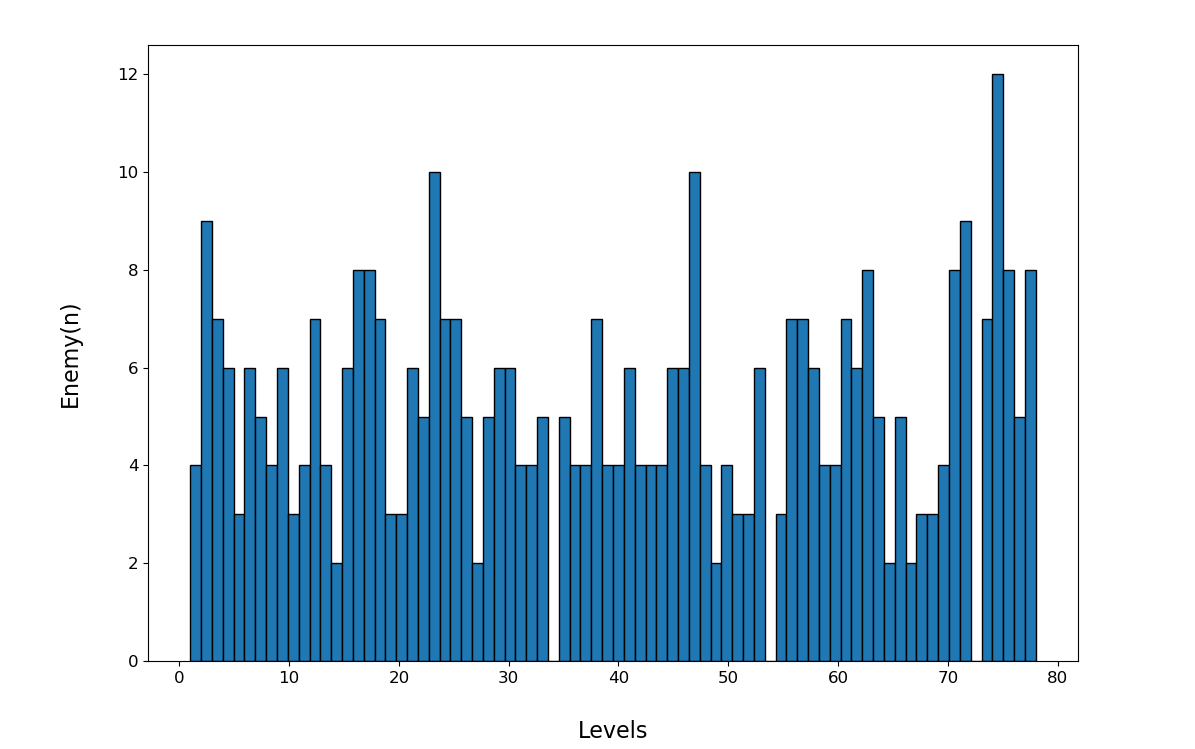
\includegraphics[scale=0.5]{img/EnemyLevelDistrib.png}
	\caption{Distribusi Level Musuh.}
	\label{fig:enemy_level_distrib}
\end{figure}
\vspace{1ex}

Selanjutnya adalah validasi dari keseimbangan persebaran level musuh, hal ini dilakukan dengan menggunakkan persamaan melalui beberapa langkah seperti yang ditunjukan oleh persamaan \ref{eq:mean_enemy_levels}, \ref{eq:varian_enemy_levels}, \ref{eq:stdev_enemy_levels} dan persamaan \ref{eq:PDF_enemy_levels}. Konsep tersebut beracuan pada Sub-bab \ref{sec:sub_sec2_gauss_bayes} tentang \textit{Gaussian Naive bayes}, dengan harapan apakah setiap data yang dihasilkan sebelumnya sudah terdistribusi dengan normal atau tidak. Adapun urutan metode dalam penggunaan \textit{Gaussian Naive Bayes} adalah dengan mencari rata-rata dari data tersebut, kemudian diikuti dengan perhitungan standar deviasi.
\vspace{1ex}

\begin{equation}\label{eq:mean_enemy_levels}
\begin{split}
\bar{E}lv = \frac{\sum_{i = 0}^{N}\ Elv_{i}}{N}
\end{split}
\end{equation}
\vspace{1ex}

Pada persamaan \ref{eq:mean_enemy_levels} adalah rata-rata dari level yang dihasilkan sama seperti pembahasan pada persamaan \ref{eq: mean} yang kemudian disimbolkan dengan variabel $\bar{E}lv$. Selanjutnya adalah $\bar{E}lv_{i}$ adalah setiap level dari musuh yang terus dijumlahkan sebanyak $N$, yang mana $N$ sendiri adalah banyaknya musuh yang sudah dibuat. Setelah diperoleh rata-rata level maka dapat dilanjutkan dengan pencarian nilai \textit{standar deviasi} seperti pada persamaan \ref{eq:stdev_enemy_levels}.
\vspace{1ex}

\begin{equation}\label{eq:varian_enemy_levels}
\begin{split}
\sigma(Elv)^2 = \frac{\sum_{i = 0}^{N}\ (Elv_{i} - \bar{E}lv)^{2}}{N}
\end{split}
\end{equation}

\begin{equation}\label{eq:stdev_enemy_levels}
\begin{split}
\sigma(Elv) = \sqrt{\frac{\sum_{i = 0}^{N}\ (Elv_{i} - \bar{E}lv)^{2}}{N}}
\end{split}
\end{equation}

Pada persamaan \ref{eq:stdev_enemy_levels} adalah persamaan untuk mencari standar deviasi atau $\sigma(Elv)$ setelah diperolehnya rata-rata atau $\bar{E}lv$ melalui persamaan \ref{eq:mean_enemy_levels} yang kemudian dilanjutkan dengan pencarian varian atau $\sigma(Elv)^2$ melalui persamaan \ref{eq:varian_enemy_levels} yang selanjutnya diakar kuadratkan untuk memperoleh nilai standar deviasi. Jika standar deviasi, varian dan rata-rata sudah diperoleh maka dapat dilanjutkan menuju pencarian nilai distribusi normal melalui \textit{Gausian Naive Bayes} seperti pada persamaan \ref{eq:PDF_enemy_levels} berikut ini.
\vspace{1ex}

\begin{equation}\label{eq:PDF_enemy_levels}
\begin{split}
PDF(ELv,\ \bar{E}lv,\ \sigma) = \frac{1}{\sqrt{2 \pi} \sigma}\ exp \left(-\frac{(Elv - \bar{E}lv)^2}{2 \sigma^2}\right)
\end{split}
\end{equation}

Konsep pada persamaan \ref{eq:PDF_enemy_levels} sudah sangat dijelaskan pada Sub-bab \ref{sec:sub_sec2_gauss_bayes} poin ke 3. Hasil perhitungaan sebelumnya yang berupa varian $\sigma^2$, rata-rata $\bar{E}lv$ dan standar deviasi $\sigma$ menjadi masukan pada persamaan tersebut. Variabel $\pi$ adalah konstanta numerik pada umumnya, kemudian fungsi $exp()$ atau $e$ adalah konstanta numerik yang betujuan untuk membentuk hasil prediksi dengan pendekatan exponensial. Jika memang benar data hasil program ini valid maka ketika musuh bertambah maka pola dari level dan jumlah musuh masih akan membentuk pola distribusi normal seperti pada Gambar \ref{fig:enemy_level_distrib_ndist}.

\begin{figure} [!h] \centering
	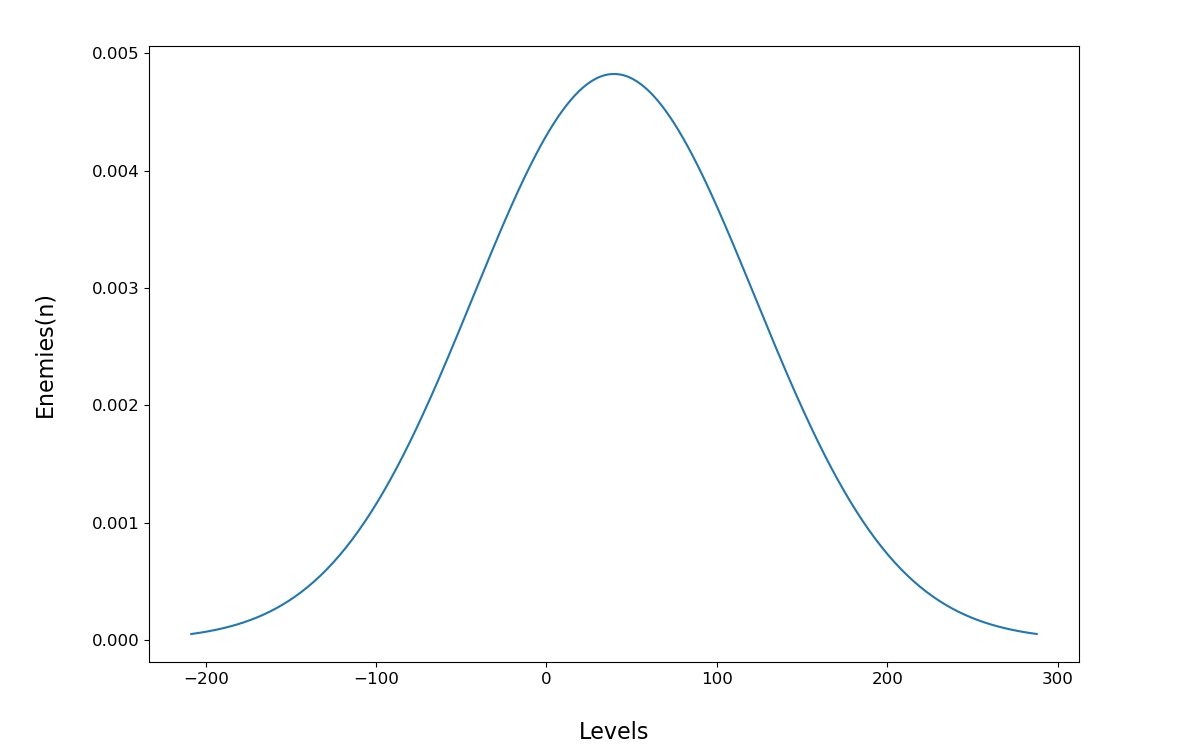
\includegraphics[scale=0.5]{img/EnemyLevelDistribNdist.png}
	\caption{Distribusi level musuh dalam bentuk distribusi normal.}
	\label{fig:enemy_level_distrib_ndist}
\end{figure}

Pada Gambar \ref{fig:enemy_level_distrib_ndist} jika dilihat persebaran datanya dari kiri ke kanan menggambarkan tingkat kesulitan musuh berdasarkan level, jumlah musuh pada sisi kiri berjumlah sedikit semakin ke kanan jumlahnya meningkat dan semakin ke kanan jumlah musuh kembali menjadi sedikit jumlahnya. Hal tersebut menggambarkan tingkat keseimbangan dari musuh yang dibuat, yang mana jumlah musuh dengan level menengah berjumlah paling banyak dan jumlah musuh yang sangat sulit dan sangat mudah dikalahkan berjummlah sedikit. Tujuan utama dari kondisi tersebut adalah terjadinya keseimbangan saat terjadinya pertarungan antara pemain dan musuh.
\vspace{1ex}

\subsection{Distribusi Tipe Musuh}
\label{sec:sub_sec3_enemy_type}
\vspace{1ex}

Di bagian distribusi tipe musuh akan dijelaskan tentang pembagian tipe musuh, dengan masukan seperti yang disebutkan pada Tabel \ref{tb:enemy_input_variable}. Beracuan pada tabel tersebut beberapa variabel utama yang akan digunakan diantaranya adalah ``\textit{Enemy Type}" yang menentukan tipe apa saja musuh yang akan dibuat. Kemudian \textit{Distribute Percentage} adalah persentase distribusi tipe yang ingin dibuat. Kemudian variabel level musuh yang diambil dan dijelaskan pada Sub-bab \ref{sec:sub_sec3_enemy_level} juga turut menentukan tipe musuh yang ingin dibuat.
\vspace{1ex}

Terdapat juga variabel pendukung yang membantu proses distribusi tipe, diantaranya adalah \textit{Distribute Number}, \textit{Distribute Level}. Kemudian dilakukan beberapa proses seperti pada persamaan \ref{eq:enemy_types_percentage}, \ref{eq:enemy_types_dist_level}, \ref{eq:enemy_types_rest_dist_level}, dan \ref{eq:enemy_rest_types} yang kemudian diperolehlah hasil berupa probabilitas distribusi tipe musuh yang ditunjukan pada persamaan \ref{eq:enemy_types_probability} dan persamaan \ref{eq:enemy_types_rest_probability}.
\vspace{1ex}

\begin{equation}\label{eq:enemy_types_percentage}
\begin{split}
	\resizebox{\columnwidth}{!}{%
		$DN_{N} = \sum_{i = 0}^{M} \sum_{j = 0}^{N}\ EN_{N} \times \frac{DP_{j}}{100}\ 
		\left\{\begin{matrix} 
		Saat\ \left \lceil DN_{i} \right \rceil - DN_{i} < DN_{i} - \left \lfloor DN_{i} \right \rfloor, & DN_{i} = \left \lceil DN_{i} \right \rceil \\ 
		Saat\ \left \lceil DN_{i} \right \rceil - DN_{i} > DN_{i} - \left \lfloor DN_{i} \right \rfloor, & DN_{i} = \left \lfloor DN_{i} \right \rfloor
		\end{matrix}\right.$%
	}
\end{split}
\end{equation}

Pada persamaan \ref{eq:enemy_types_percentage} adalah persamaan untuk mencari \textit{distribute number} atau distribusi musuh $DN_{N}$ yang mana nilai dari variabel tersebut akan memiliki nilai sebenarnya yang diperoleh melalui jumlah musuh $EN_{N}$ yang sudah dibahas pada Sub-bab \ref{sec:sub_sec3_enemy_level}, yang kemudian dibandingan dengan presentase yang disiapkan sebelumnya melalui variabel masukan \textit{distribute percentage} atau $DP_{j}$ dengan nilai yang ditunjukan pada Tabel \ref{tb:enemy_input_variable}. Keluaran dari $DN_{N}$ sendiri berupa angaka bulat dan berupa \textit{cluster} angka, maka dari itu setiap angka yang membentuk \textit{cluster} jumlah musuh tersebut harus dilakukan operasi pembulatan seperti pada $DN_{N}$ dengan menggunakan syarat seperti pada persamaan \ref{eq:enemy_types_percentage}. Selain itu angka bulat yang dihasilkan jumlahnya tidak hanya berjumlah satu, pemecahan jumlah musuh pada bagian ini mengikuti jumlah angka yang ada dalam variabel $DP_{j}$. Secara berurutan jumlah angka tersebut merealisasikan persentase jumlah tipe musuh pada variabel $DP_{j}$.
\vspace{1ex}

\begin{equation}\label{eq:enemy_types_dist_level}
\begin{split}
	DL_{N} = \sum_{i = 0}^{M} \sum_{j = 0}^{N} \left \lfloor \frac{DN_{j}}{DP_{i}} \right \rfloor\
	\left\{\begin{matrix} 
	Saat\ i = 0, & \hspace{-4.0em}DL_{i} = DN_{i} \\ 
	\hspace{0.5em} Lainnya, & DL_{i - 1} < DL_{(i - 1) + DN}
	\end{matrix}\right.
\end{split}
\end{equation}

Selanjutnya adalah operasi pembagian musuh dan levelnya setelah ditemukannya $DN_{N}$, sebagai batasan dalam membagi setiap musuh berdasarkan presentase tipe $DP_{N}$ pada persamaan \ref{eq:enemy_types_dist_level}. Dengan kata lain $DP_{N}$ digunaan sebagai pembagi jumlah musuh ke dalam level, padalah $DP_{N}$ adalah sebuah variabel yang bertujuan memuat presentase pembagian jumlah musuh dan level saja. Hal ini bersifat opsional dan dapat terus dikembangkan mungkin dengan menambah variabel baru untuk mendistribusikan jumlah musuh ke dalam level dengan tidak menggunakan variabel $DP_{N}$.
\vspace{1ex}

Kemudian pada persamaan \ref{eq:enemy_types_dist_level} dicarilah nilai $DL_{N}$ yang berisi urutan distribusi musuh $DN_{i}$ yang dibagi dengan jumlah presentase tipe $DP_{N}$ seperti pada persamaan \ref{eq:enemy_types_percentage}. Hal tersebut sejatinya akan membentu sebuah \textit{cluster} kecil yang berisi distribusi musuh dan tipenya. Bila membagi setiap musuh dengan jumlah presetase tipe maka tidak semua musuh dapat terbagi secara merata atau habis, maka dari itu juga dicari sisa hasil pembagian antara distribusi musuh $DN_{i}$ dengan jumlah presentase tipe $DP_{N}$ pada persamaan \ref{eq:enemy_types_rest_dist_level} pada persamaan \ref{eq:enemy_types_rest_dist_level}.
\vspace{1ex}

\begin{equation}\label{eq:enemy_types_rest_dist_level}
rDL_{N} \equiv \sum_{i = 0}^{N}\ DN_{i}\ (mod\ DP_{N})
\end{equation}

Pada persamaan \ref{eq:enemy_types_rest_dist_level} diperolehlah sisa musuh yang tidak terdistribusi atau sisa dari jumlah musuh yang tidak habis saat dibagi dengan jumlah presentase tipe $DP_{N}$. Musuh yang belum terdistribusi nantinya akan ditambahan atau didistribusi ke tipe sesuai urutan hasil yang tersimpan pada variabel \ref{eq:enemy_types_rest_dist_level} pada persamaan \ref{eq:enemy_types_rest_dist_level}.

\begin{equation}\label{eq:enemy_types_probability}
P(ET_{i}) = \sum_{i = 0}^{M} \sum_{j = 0}^{N}\ \frac{ET_{i}}{\sum_{k = 0}^{L}DL_{k}}\
\left\{\begin{matrix}
\hspace{-4.6em} Saat\ ET_{i} \leq DL_{j} \\ 
Saat\ DL_{(j-1)} < ET_{i} \leq DL_{j}
\end{matrix}\right.
\end{equation}

Dari jumlah musuh yang terdistribusi kedalam \textit{cluster} level tersebutlah kemudian dilakukan pemetaan tipe, pada kasus ini digunakanlah konsep probabilitas marginal seperti yang dijelaskan pada persamaan \ref{sec:sub_sec2_bayes} poin ke 1, bila disesuaikan dengan kasus ini maka persamaan yang diperoleh akan menjadi seperti pada persamaan \ref{eq:enemy_types_probability}. Pada setiap karakter musuh $ET_{i}$ akan meilih satu tipe yang akan digunakannya, tipe tersebut akan menentukan \textit{stats} atau data statistiknya yang akan dijelaskan pada bagian selanjutnya. Kemudian probabilitas tipe yang dipilih $ET_{i}$ dinyatakan dengan variabel $P(ET_{i})$, kisaran kemunculan nilai atau tipe musuh $ET_{i}$ diperoleh dari sekumpulan data distribusi level $DL_{N}$.

\begin{equation}\label{eq:enemy_rest_types}
rET = \sum_{i = 0}^{M} \sum_{j = 0}^{N}\ EN_{M} - ET_{N}
\end{equation}

Selanjutnya pada persamaan \ref{eq:enemy_rest_types} adalah langkah untuk melihat apakah ada sisa musuh yang belum terdistribusi $rET$ dengan cara melakukan pengurangaan antara jumlah musuh $EN_{M}$ yang sudah dijelaskan pada Sub-bab \ref{sec:sub_sec3_enemy_level}, yang mana $M$ pada variabel tersebut menandakan jumlah musuh sedangan $ET$ adalah tipe dengan  $N$ sebagai jumlah musuh yang sudah memiliki tipe. 
\vspace{1ex}

Pada persamaan \ref{eq:enemy_rest_types} variabel $rET$ dapat bernilai 0 saat semua musuh $DN$ habis terbagi kedalam jumlah presentase dari tipe $DP_{N}$ seperti pada persamaaan \ref{eq:enemy_types_dist_level} dengan sisa musuh yang belum terdistribusi atau memiliki level disimpan pada variabel $rDL_{N}$ pada persamaan \ref{eq:enemy_types_rest_dist_level}. Kemudian selanjutnya adalah mendistribusikan sisa musuh yang belum memilliki tipe tersebut, seperti yang dilakukan oleh persaman \ref{eq:enemy_types_rest_probability}.
\vspace{1ex}

\begin{equation}\label{eq:enemy_types_rest_probability}
	P(ET_{i}) = \sum_{i = 0}^{M} \sum_{j = 0}^{N}\ \frac{ET_{i}}{\sum_{k = 0}^{L}\ rDL_{k}}\
	\left\{\begin{matrix}
	\hspace{-5.0em} Saat\ ET_{i} \leq rDL_{j}, rET > 0\\
	\hspace{0.5em} Saat\ rDL_{(j-1)} < ET_{i} \leq rDL_{j},\ rET > 0\\
	\hspace{-12.5em} Lainnya\ 0
	\end{matrix}\right.
\end{equation}

Melanjutkan persamaan \ref{eq:enemy_types_rest_probability}, yang mana didistribusikan sisa musuh yang belum terdistribusi $rDL_{N}$. Kemudian setelah didistribusikan atau memilih tipe $ET_{i}$ hasilnya digabung dengan tipe musuh yang sudah terdistribusi sebelumnya. Sama seperti pada persaamaan \ref{eq:enemy_types_probability} variabel $P(ET_{i})$ adaalah probabilitas tipe musuh yang dipilihh dari distribusi level $rDL_{k}$. Hasil distribusi dan penjeasan level yang dilakukan oleh beberapa persamaan diatas, maka hasilnya akan menjadi seperti Tabel \ref{tb:enemy_type_distrib}.
\vspace{1ex}

\begin{table}[!h]
	\centering
	\caption{Hasil level yang dibuat untuk musuh.}
	\label{tb:enemy_type_distrib}
	\begin{tabular}{|l|l|l|l|}
		\hline
		\textbf{No.} & \textbf{Name} & \textbf{Levels} & \textbf{Type} \\ \hline
		1 & Enemy 1 & 1 & 0 \\ \hline
		2 & Enemy 2 & 1 & 0 \\ \hline
		3 & Enemy 3 & 1 & 2 \\ \hline
		4 & Enemy 4 & 1 & 1 \\ \hline
		5 & Enemy 5 & 2 & 2 \\ \hline
		6 & Enemy 6 & 2 & 1 \\ \hline
		7 & Enemy 7 & 2 & 2 \\ \hline
		8 & Enemy 8 & 2 & 0 \\ \hline
		9 & Enemy 9 & 2 & 2 \\ \hline
		10 & Enemy 10 & 2 & 2 \\ \hline
		11 & Enemy 11 & 2 & 4 \\ \hline
		12 & Enemy 12 & 2 & 0 \\ \hline
		13 & Enemy 13 & 2 & 0 \\ \hline
		14 & Enemy 14 & 3 & 4 \\ \hline
		15 & Enemy 15 & 3 & 4 \\ \hline
		... & ... & ... & ... \\ \hline
		\textbf{400} & \textbf{Enemy 400} & \textbf{78} & \textbf{3} \\ \hline
	\end{tabular}
\end{table}
\vspace{1ex}

Dari data yang tedapat pada Tabel \ref{tb:enemy_type_distrib} hanya sebagian data saja, lebih lengkapnya dapat dilihat langsung pada Bagian \nameref{chap:chap6_attachment} dalam Tabel \ref{tb:enemies_all_stats_1} sampai dengan Tabel \ref{tb:enemies_all_stats_15} di kolom \textit{Type}. Pada Tabel \ref{tb:enemy_type_distrib} dan tabel lain yang memuat tentang \textit{Type} yang berisi data $ET_{i}$ atau jenis musuh yang diisi dengan angka 0 sampai dengan 4, maksud dari angka tersebut adalah untuk mewakili indeks dari variabel \textit{Enemy Type} pada Tabel \ref{tb:enemy_input_variable}. Secara berurutan dari 0 sampai dengan 4 adalah \textit{Mixed}, \textit{Hard Magic}, \textit{Soft Magic}, \textit{Hard Strength}, dan \textit{Soft Magic}. Seluruh data tersebut jika divisualisasikan maka hasilnya seperti Gambar \ref{fig:enemy_type_distrib} sesuai yang ditargetkan oleh variabel \textit{Distribute Percentage} pada Tabel \ref{tb:enemy_input_variable} atau variabel $DP$ pada persamaan \ref{eq:enemy_types_percentage}.

\begin{figure} [!h] \centering
	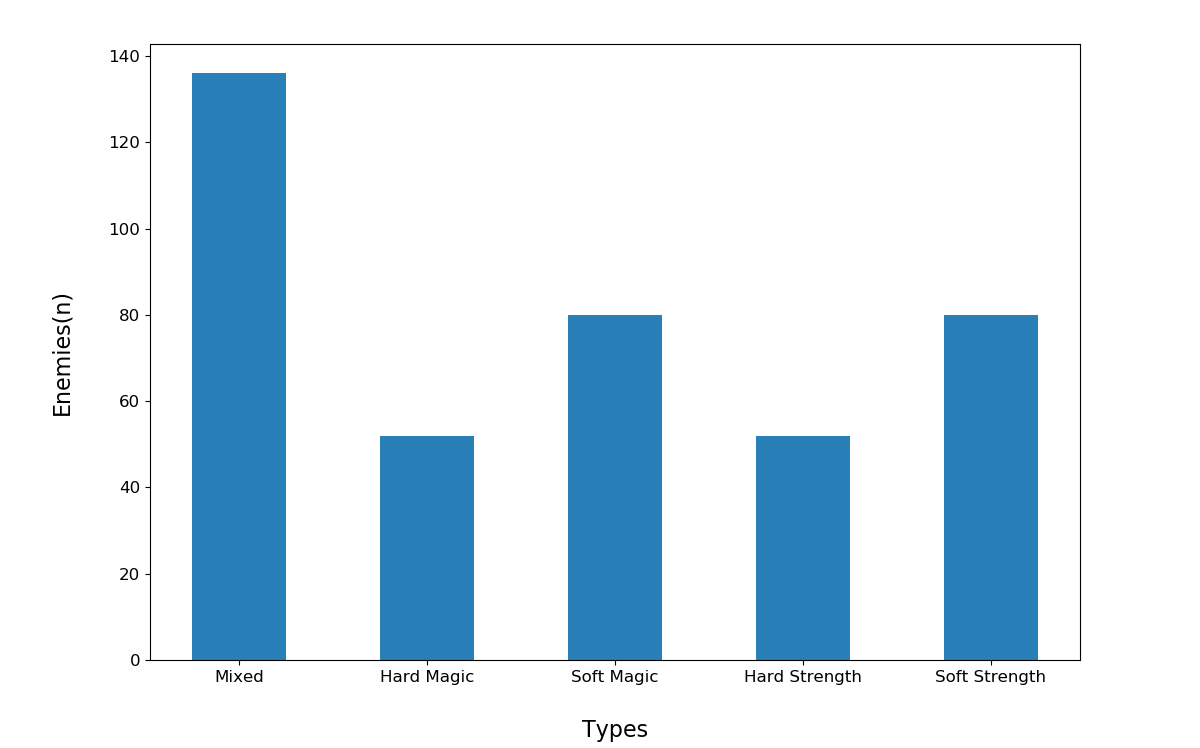
\includegraphics[scale=0.5]{img/EnemyTypeDistrib.png}
	\caption{Distribusi tipe musuh.}
	\label{fig:enemy_type_distrib}
\end{figure}

Kemudian pada Gambar \ref{fig:enemy_type_distrib} adalah hasil dari proses pembuatan dan pengelompokan musuh berdasarkan tipe yang sudah sesuai dengan variabel masukan pada Tabel \ref{tb:enemy_input_variable}. Dengan musuh bertipe \textit{Mixed} berjumlah yang paling banyak, diikuti \textit{soft magic} dan \textit{soft strength} dengan harapan bahwa ini adalah musuh yang memiliki karakter \textit{magic} dan \textit{strength} namun masih mudah dikalahkan, dilanjutkan dengan yang paling sedikit adalah \textit{hard magic} dan \textit{hard strength} dengan harapan menjadi musuh berkarakter strength dan magic yang sulit dikalahkan.
\vspace{1ex}

\subsection{Distribusi Elemen dan Kelemahan Musuh}
\label{sec:sub_sec3_enemy_weak}
\vspace{1ex}

Pada persamaan \ref{eq:enemy_element} adalah penjelasan elemen yang digunakan oleh musuh seperti dideskripsikan pada Tabel \ref{tb:enemy_input_variable} pada variabel \textit{List Element}, di mana pada elemen teresebut terdapat kelemahan atau \textit{weaknesses} dan kekebalan atau \textit{repel} seperti yang dideskripsikan pada variabel \textit{List Damage} pada Tabel \ref{tb:enemy_input_variable}.  Seperti yang dijelaskan pada Sub-bab \ref{sec:sub_sec3_design_skenario} poin ke dua tentang Elemen dan Efektifitas Serangan. Pada bagian ini elemen tersebut akan dibagi ke setiap musuh dengan kondisi yang berbeda, maksudnya nanti akan ada musuh yang memiliki kelemahan dan kekebalan yang berbeda antara musuh satu dengan musuh yang lain. Misalkan \textit{Enemy 1} memiliki kelemahan api atau \textit{fire} yang mana HP akan berkurang dua kali jika diserang dengan menggunakan elemen api dan memiliki kekebalan air atau \textit{water} yang mana karakter tersebut kebal saat diserang dengan \textit{skill} dari elemen air. Kemudian pada \textit{Enemy 2} berbeda dengan \textit{Enemy 1}, misalnya pada \textit{Enemy 1} memiliki kelemahan api sedangkan pada \textit{Enemy 2} memiliki kelemahan air misal dan kebal terhadap angin atau \textit{wind}.

\begin{equation}\label{eq:enemy_element}
\resizebox{0.2\textwidth}{!}{%
	$ElN = \left\{\begin{matrix}
	\hspace{-0.34em} Phys \\ 
	\hspace{0.3em} Water \\
	\hspace{0.0em} Wind \\
	\hspace{0.2em} Earth \\
	\hspace{-0.3em} Fire \\
	\hspace{-1.6em} ... \\
	\hspace{-1.6em} n
	\end{matrix}\right.$%
}
\end{equation}

Pada dasarnya satu karakter musuh tidak akan menggunakan seluruh elemen yang ada pada persamaan \ref{eq:enemy_element} yang merupakan penggambaran dari varaibel \textit{List Element} pada Tabel \ref{tb:enemy_input_variable}, mungkin hanya sekitar satu sampai dengan tiga. Maka dari itu kondisi tersebut dapat dinyatakan dengan kondisi $DmgNa \in ElN$, yang mana seluruh elemen bisa menjadi kelemahan atau kekebalan dari musuh. Sama seperti pada persamaan \ref{eq:enemy_element} yang mana $ElN$ adalah nama elemen, sedangkan $DmgNa$ adalah \textit{damage name} atau nama dari efek serangan yang dilakukan. Di mana pada persamaan \ref{eq:damage_name_number} $DmgNa$ akan dipilih secara acak dengan persamaan \ref{eq:damage_number_prob}, yang akan menjadi kelemahan atau kekebalan terhadap serangan dari pemain seperti pada persamaan \ref{eq:damage_name_number}. Pada persamaan \ref{eq:damage_name_number} sendiri adalah penggambaran dari variabel \textit{List Damage} pada Tabel \ref{tb:enemy_input_variable}. 

\begin{equation}\label{eq:damage_name_number}
\resizebox{0.5\textwidth}{!}{%
	$DmgNu = \left\{\begin{matrix} 
	\hspace{0.0em} 0,  & \hspace{-7.0em} Normal \\
	\hspace{0.0em} 1,  & \hspace{-8.0em} Repel \\
	\hspace{0.0em} 2,  & \hspace{-7.7em} Weak \\
	\hspace{0.5em} ... & \\
	\hspace{0.5em} n,  & Defined\ Status\ Name
	\end{matrix}\right.$%
}
\end{equation}

Sedangkan pada persamaan \ref{eq:damage_name_number} variabel $DmgNu$ adalah respon terhadap serangan yang yang dikonversi menjadi angka, yang pada mulanya berupa nama respon atau status setelah diserang. Kemudian hasil pemilihan tersebut disimpan pada variabel $DmgNu$ yang dapat dinyatakan dengan persamaan \ref{eq:damage_number_prob}.

\begin{equation}\label{eq:damage_number_prob}
P(DmgNu) = \frac{DmgNu}{\sum_{i = 0}^{N} DmgNa_{(i - 1)}}
\end{equation}

Pada persamaan \ref{eq:damage_name_number} variabel $DmgNa$ yang dipilih secara acak sebagai elemen yang memiliki respon khusus terhadap serangan yang kemudian disimpan pada variabel $DmgNu$, selanjutnya angka yang dipilih akan disimpan pada variabel $DmgNu$ yang selanjutnya dinyatakan dengan persamaan \ref{eq:damage_number_prob}. Jadi dari $DmgNa$ akan dipilih satu sampai dengan tiga elemen secara acak yang kemudian menjadi kelemahan atau kekebalan dari karakter musuh tersebut.

\begin{equation}\label{eq:multi_damage_num_prob}
P(DmgNu)_{M} = \sum_{i = 0}^{M} \frac{DmgNu_{i}}{\sum_{j = 0}^{N} DmgNa_{j - 1}}
\end{equation}

Sedangkan pada persamaan \ref{eq:multi_damage_num_prob} adalah penjelasan tentang proses munculnya setiap $DmgNu$ pada satu karakter musuh, sehingga variabel tersebut berubah menjadi $DmgNu_{i}$. Seperti penjelasan sebelumnya bahwa pada sebuah karakter musuh dapat memiliki lebih dari satu kelemahan atau kekebalan $DmgNu$ terhadap $DmgNa$ yang diset secara acak seperti yang sudah dijelaskan pada bagian sebelumnya.

\begin{equation}\label{eq:all_enemies_damage}
DmgEN_{M} = \sum_{i = 0}^{M}\sum_{j = 0}^{N} DmgNu_{ij}
\end{equation}

Selanjutnya adalah proses penerapan persamaan \ref{eq:multi_damage_num_prob} ke seluruh karakter musuh $DmgEN_{M}$ seperti pada persamaan \ref{eq:all_enemies_damage}. Sesuai dengan persamaan \ref{eq:all_enemies_damage} yang mana $M$ adalah jumlah musuh sedangkan $N$ adalah jumlah $DmgNu$ pada satu musuh yang berjumlah satu sampai dengan tiga seperti yang sudah dijelaskan pada paragraf sebelumnya Sub-bab ini. Hasil dari proses yang sebelumnya dijelaskan pada Sub-bab ini menghasilkan persebaran kelemahan dan kekebalan musuh yang ditunjukkan pada Gambar \ref{fig:enemy_weak_distrib} dibawah ini.

\begin{figure} [!h] \centering
	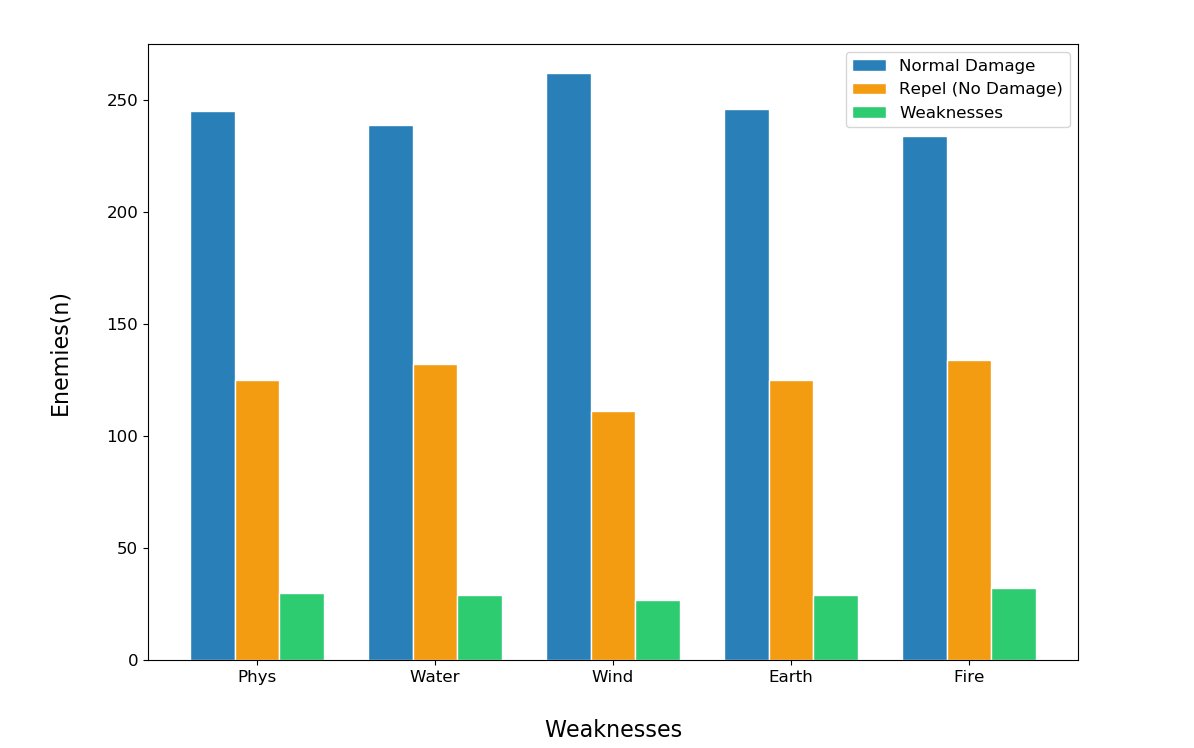
\includegraphics[scale=0.50]{img/EnemyWeakDistrib.png}
	\caption{Distribusi kelemahan musuh.}
	\label{fig:enemy_weak_distrib}
\end{figure}

Pada Gambar \ref{fig:enemy_weak_distrib} dapat dilihat distribusi musuh dengan kelemahan dan kekebalannya. Terlihat pada kondisi tersebut jumlah musuh dengan kondisi \textit{Normal} memiliki nilai paling tunggi pada setiap kelemahan, hal tersebut dapat diartikan bahwa sebagian besar elemen dari musuh dapat memperoleh \textit{damage} secara normal jika diserang. Kemudian jumlah musuh pada kondisi \textit{Repel} berjumlah terbanyak kedua, hal tersebut dapat diartikan musuh memmiliki jumlah kekebalan terhadap serangan sejumlah angka pada setiap elemen pada Gambar \ref{fig:enemy_weak_distrib}. Begitu juga dengan kondisi \textit{Weaknesses} dengan jumlah paling sedikit, hal tersebut bertujuan agar menjadikan pertarungan antara pemain dan musuh menjadi tidak mudah dimenangkan oleh pemain. Tidak hanya dengan efek \textit{Weaknesses}, efek \textit{Repel} juga sangat berpengaruh dalam menjadikan permainan seperti layaknya sebuah \textit{puzzle} atau teka-teki.
\vspace{1ex}

Sedangkan pada persamaan \ref{eq:multi_damage_num_prob} adalah penjelasan tentang proses munculnya setiap $DmgNu$ pada satu karakter musuh, sehingga variabel tersebut berubah menjadi $DmgNu_{i}$. Seperti penjelasan sebelumnya bahwa pada sebuah karakter musuh dapat memiliki lebih dari satu kelemahan atau kekebalan $DmgNu$ terhadap $DmgNa$ yang diset secara acak seperti yang sudah dijelaskan pada bagian sebelumnya. 
\vspace{1ex}

\subsection{Distribusi HP, MP dan Stats Musuh}
\label{sec:sub_sec3_enemy_hp_mp_stats}
\vspace{1ex}

Bila melihat pada Tabel \ref{tb:enemy_input_variable} terdapat beberapa variabel seperti \textit{List Stats Name}, \textit{Max Stats Value}, dan \textit{Min Stats Value}. Variabel tersebut akan digunakan untuk membuat \textit{stats} dari musuh dengan basis algorima Naive Bayes. Di awali dengan persamaan \ref{eq:enemy_types_stats_ex} yang menjadi pembagi setiap operasi pembagian \textit{stats} berdasarkan tipenya $ET_{i}$.

\begin{equation}\label{eq:enemy_types_stats_ex}
\resizebox{0.4\textwidth}{!}{%	
	$ET_{N} = \sum_{i= 0}^{N} ET_{i} \left\{\begin{matrix}
	ET_{i} = 0, & MX\\ 
	ET_{i} = 1, & HM\\ 
	ET_{i} = 2, & SM\\ 
	ET_{i} = 3, & HS\\ 
	ET_{i} = 4, & SS
	\end{matrix}\right.$%
}
\end{equation}

Pada persamaan \ref{eq:enemy_types_stats_ex} adalah persamaan yang disesuaikan untuk menyelesaikan masukan variabel pada Tabel \ref{tb:enemy_input_variable}, sedangkan pada persaamaan \ref{eq:enemy_types_stats_adv} adalah pengembangan jika jumlah tipe musuh dinaikkan lebih dari yang dicontohkan pada Tabel \ref{tb:enemy_input_variable} pada variabel \textit{Enemy Type}.
\vspace{1ex}

\begin{equation}\label{eq:enemy_types_stats_adv}
\resizebox{0.4\textwidth}{!}{%
	$ET_{N} = \sum_{i= 0}^{N} ET_{i} \left\{\begin{matrix}
	ET_{i} = 0, & MX\\ 
	ET_{i} = 1, & HM\\ 
	ET_{i} = 2, & SM\\ 
	ET_{i} = 3, & HS\\ 
	ET_{i} = 4, & SS\\
	... & ... \\
	\hspace{0.2em} ET_{n} = n, & ST_{n}
	\end{matrix}\right.$%
}
\end{equation}

Pada kedua persamaan tersebut terdaapat beberapa variabel diantaranya adalah $ET_{i}$ yang merupakan enemy tipe ke $i$, kemudian secara berurutan masing-masing $MX$, $HM$, $SM$, $HS$, dan $SS$ adalah musuh dengan tipe \textit{mixed}, \textit{hard magic}, \textit{soft magic}, \textit{hard strength}, dan \textit{soft strength}. Kemudian pada persamaan \ref{eq:enemy_types_stats_adv} secara spesifik terdapat variabel $ET_{n}$ yang merupakan variabel tipe musuh ke $n$ atau batas jumlah musuh. Variabel $n$ adalah urutan dari index tipe musuh yang dideskripsikan, berikut juga variabel $ST_{n}$, dengan variabel $ST$ adalah \textit{stats} dan $n$ adalah batas jumlah musuh. Selanjutnya adalah dilakukannya pembagian tipe musuh jika musuh tersebut memiliki tipe $MX$ atau \textit{mixed} seperti pada persamaan \ref{eq:enemy_types_stats_mixed_ex}.
\vspace{1ex}

\begin{equation}\label{eq:enemy_types_stats_mixed_ex}
MX_{N} = \sum_{i= 0}^{N} MX_{i} \left\{\begin{matrix}
MX_{i} = 1, & MP\ Focused\\
MX_{i} = 2, & HP\ Focused
\end{matrix}\right.
\end{equation}

Pada persamaan \ref{eq:enemy_types_stats_mixed_ex} terdapat variabel $MX_{i}$ yang merupakan variabel satuan dari musuh yang bertipe \textit{mixed}. Kemudian pada variabel $MX_{N}$ adalah variabel yang bersifat jamak atau memuat banyak variabel musuh yang bertipe \textit{mixed}. Pada persamaan \ref{eq:enemy_types_stats_mixed_ex} sendiri dijelaskan bahwa pada tipe \textit{mixed} dipecah menjadi dua tipe lagi, yang satu berfokus pada $HP$ dan satu lagi pada $MP$. Jadi isi dari variabel $MX_{N}$ nantinya akan terdiri dari musuh bertipe \textit{mixed} dengan sub-tipe MP atau berfokus pada MP dan sub-tipe HP atau berfokus pada HP.

\begin{equation}\label{eq:enemy_types_stats_mixed_adv}
Mx_{N} = \sum_{i= 0}^{N} Mx_{i} \left\{\begin{matrix}
\hspace{0.6em} Mx_{i} = 1, & MP\ Focused\\
\hspace{0.6em} Mx_{i} = 2, & HP\ Focused\\
\hspace{0.6em} ... & \hspace{-2.0em} ... \\
\hspace{0.8em} Mx_{N} = n, & \hspace{-2.0em} Lainnya\\
\end{matrix}\right.
\end{equation}

Selanjutnya adalah perhitungan probabilitas diperolehnya tipe musuh dari keseluruhan tipe musuh yang berada pada variabel masukan. Misal pada kasus yang ditunjukan pada persamaan \ref{eq:enemy_types_prob_ex}, jumlah tipe musuh tentunya mengacu pada Tabel \ref{tb:enemy_input_variable}. Dalam menyelesaikan kasus tersebut digunakanlah Naive bayes yang berbasis pada \textit{conditional probability} seperti yangg dijelaskan pada Sub-bab \ref{sec:sub_sec2_class_bayes}, yang mana pada persamaan \ref{eq:enemy_types_prob_ex} proses kemunculan tipe musuh tertentu misal $ET_{0}$, $ET_{1}$, $ET_{2}$, $ET_{3}$, $ET_{4}$ yang mana seluruh tipe musuh dimuat pada variabel $ET_{N}$.

\begin{equation}\label{eq:enemy_types_prob_ex}
\resizebox{0.35\textwidth}{!}{%
	$\begin{matrix}
	ET_{0} = P(ET_{N}| ET_{0}) \times P(ET_{0})\\
	ET_{1} = P(ET_{N}| ET_{1}) \times P(ET_{1})\\
	ET_{2} = P(ET_{N}| ET_{2}) \times P(ET_{2})\\
	ET_{3} = P(ET_{N}| ET_{3}) \times P(ET_{3})\\
	ET_{4} = P(ET_{N}| ET_{4}) \times P(ET_{4})
	\end{matrix}$%
}
\end{equation}

Sedangkan jika jumlah tipe musuh tidak beracuan pada Tabel \ref{tb:enemy_input_variable} atau tipe musuh berjumlah lebih dari empat maka persamaan \ref{eq:enemy_types_prob_ex} akan berubah menjadi persamaan \ref{eq:enemy_types_prob_adv}. Semula berawal dari variabel $ET_{0}$ sampai $ET_{4}$ pada persamaan \ref{eq:enemy_types_prob_ex} yang kemudian berubah dari variabel $ET_{0}$ sampai $ET_{n}$ dengan $n$ adalah batas akhir jumlah tipe musuh.

\begin{equation}\label{eq:enemy_types_prob_adv}
\resizebox{0.35\textwidth}{!}{%
	$\begin{matrix}
	ET_{0} = P(ET_{N}| ET_{0}) \times P(ET_{0})\\
	ET_{1} = P(ET_{N}| ET_{1}) \times P(ET_{1})\\
	ET_{2} = P(ET_{N}| ET_{2}) \times P(ET_{2})\\
	...\\
	ET_{n} = P(ET_{N}| ET_{n}) \times P(ET_{n})
	\end{matrix}$%
}
\end{equation}

Saat sudah diperolehnya tipe musuh pada seperti yang dijelaskan pada persamaan \ref{eq:enemy_types_prob_adv} maka selanjutnya yang harus dibuat adalah stats dari musuh itu sendiri, seperti halnya HP, MP, Strength, Magic dan lain sebagainya seperti yang tercantum pada Tabel \ref{tb:enemy_input_variable} pada variabel $List Stats Name$ yang ditambah dengan variabel HP dan MP.

\begin{equation}\label{eq:enemy_types_prob_bhp}
bHP = minHP
\end{equation}

Pada persamaan \ref{eq:enemy_types_prob_bhp} adalah penentuan batas bawah untuk HP atau $bHP$, nilai $minHP$ juga dicontohkan dalam daftar variabel masukan dengan nama \textit{Min} HP pada Tabel \ref{tb:enemy_input_variable}.

\begin{equation}\label{eq:enemy_types_prob_thp}
tHP = \sum_{i=0}^{N}\ bHP + \left |\ \frac{Elv_{i}}{100} \times maxHP\ \right |
\end{equation}

Selanjutnya dilanjutkan dengan pencarian batas atas untuk HP atau $tHP$. Pada persamaan \ref{eq:enemy_types_prob_thp} terdapat beberapa variabel yang berpengaruh terhadap nilai dari $tHP$ diantaranya adalah $bHP$ yang merupakan batas bawah dari $HP$, $Elv_{i}$ yang merupakan level dari setiap karakter musuh dengan tipenya masing-masing, dan $maxHP$ sendiri yang merupakan batas atas dicontohkan pada Tabel \ref{tb:enemy_input_variable} dengan nama variabel $max$ HP. Pencarian batas atas dilakukan dengan dilakukannya penjumlahan antara $bHP$ dengan presentase dari $maxHP$ yang disesuaikan dengan $Elv_{i}$. Jadi dari perhitungan tersebut HP dari karakter musuh akan menyesuikan dengan level pada karakter musuh tersebut. 

\begin{equation}\label{eq:enemy_types_prob_hp}
P(HP_{i}) = \sum_{i=0}^{N}\ \frac{HP_{i}}{bHP_{i} - tHP_{i}}
\end{equation}

Kemdian dilanjutkan dengan perhitungan probabilitas $P(HP_{i})$ atau munculnya HP pada setiap karakter musuh pada persamaan \ref{eq:enemy_types_prob_hp}. HP dari setiap karakter musuh itu sendiri dinyatakan dengen $HP_{i}$. Kemudian range nilai dari $HP_{i}$ yang akan muncul terhitung mulai dari $bHP_{i}$ sampai dengan $tHP_{i}$ dari setiap karakter musuh. Variabel $i$ pada persamaan tersebut merepresentasikan setiap musuh dengan variabel $N$ yang menyatakan batas atau jumlah dari musuh yang ingin dibuat.

\begin{equation}\label{eq:enemy_types_prob_bmp}
bMP = minMP
\end{equation}

Mengulang persamaan \ref{eq:enemy_types_prob_bhp} pada persamaan \ref{eq:enemy_types_prob_bmp}, hanya mengganti variabelnya saja. Jika pada persamaan \ref{eq:enemy_types_prob_bhp} kasus yang ingin diselesaikan adalah pencariaan \textit{stats} HP, maka pada persamaan \ref{eq:enemy_types_prob_bmp} kasus yang ingin diselesaikan adalah pencarian \textit{stats} MP. Pada persamaan \ref{eq:enemy_types_prob_bhp} dengan variabel $bHP$ diganti dengan $bMP$ dan variabel $minHP$ diganti dengan $minMP$ yang mana pada Tabel \ref{tb:enemy_input_variable} dicontohkan dengan variabel $Min$ MP.
\vspace{1ex}

\begin{equation}\label{eq:enemy_types_prob_tmp}
tMP = \sum_{i=0}^{N}\ bMP + \left |\ \frac{Elv_{i}}{100} \times maxMP\ \right |
\end{equation}

Masih sama seperti penjelasan sebelumnya dimana pada persaamaan \ref{eq:enemy_types_prob_bmp} pada persamaan \ref{eq:enemy_types_prob_tmp} juga sama dengan persamaan \ref{eq:enemy_types_prob_thp}. Di lakukannya penggantian variabel HP menjadi MP, sudah dijelaskan juga pada bagian sebelumnya tentang variabel $Elv_{i}$, dan pada variabel $maxMP$ yang merupakan variabel yang dicontohkan pada Tabel \ref{tb:enemy_input_variable} dengan nama \textit{Max} MP.

\begin{equation}\label{eq:enemy_types_prob_mp}
P(MP_{i}) = \sum_{i=0}^{N}\ \frac{MP_{i}}{bMP_{i} - tMP_{i}}
\end{equation}

Pada persamaan \ref{eq:enemy_types_prob_mp} adalah probabilitas $P(MP_{i})$ atau munculnya MP pada setiap karakter musuh pada persamaan \ref{eq:enemy_types_prob_mp}. MP dari setiap karakter musuh itu sendiri dinyatakan dengen $MP_{i}$. Kemudian range nilai dari $MP_{i}$ yang akan muncul terhitung mulai dari $bMP_{i}$ sampai dengan $tMP_{i}$. Kasus ini sama seperti pada persamaan \ref{eq:enemy_types_prob_hp} hanya saja sama seperti pada pembahasan sebelumnya yang mana pada persamaan tersebut bertujuan untuk mencari $HP$, sedangkan pada kasus ini bertujuan untuk mencaru $MP$.
\vspace{1ex}

Pada bagian ini akan membahas secara khusus untuk kondisi \textit{mixed} melanjutkan seperti yang ada pada persamaan \ref{eq:enemy_types_stats_mixed_ex}. Dalam kondisi \textit{mixed} sendiri terdapat dua kondisi yaitu HP \textit{focused} atau yang berfokus kepada HP, kemudian MP \textit{focused} atau yang befokus pada MP. Bila masing-masing tipe tersebut dinyatakan dengan persamaan secara berurutan untuk HP \textit{focused} dan MP \textit{focused} dengan persamaan \ref{eq:enemy_types_prob_mx1} dan persamaan \ref{eq:enemy_types_prob_mx2}. 

\begin{equation}\label{eq:enemy_types_prob_mx1}
Mx_{1} = P(Mx_{{N}}|Mx_{1}) \times P(Mx_{1})
\end{equation}

Maka $Mx_{N}$ adalah seluruh musuh yang bertipe $mixed$, kemudian dipilihlah musuh dengan tipe mixed yang berfokus pada HP atau $Mx_{1}$. Beracuan pada konsep \textit{conditional probability} yang sudah dijelaskan pada Sub-bab \ref{sec:sub_sec2_bayes}.

\begin{equation}\label{eq:enemy_types_prob_mx2}
Mx_{2} = P(Mx_{{N}}|Mx_{2}) \times P(Mx_{2})
\end{equation}

Jika $Mx_{1}$ adalah HP \textit{focused} maka  $Mx_{2}$ adalah MP \textit{focused} maka sama seperti persamaan \ref{eq:enemy_types_prob_mx1} dengan $Mx_{N}$ adalah seluruh musuh yang bertipe $mixed$, kemudian dipilihlah musuh dengan tipe \textit{mixed} yang berfokus pada MP atau $Mx_{2}$. Pembahasan secara khusus lainnya adalah penambahan \textit{stats} HP untuk musuh dengan tipe \textit{mixed} yang berfokus pada HP seperti yang dinyatakan pada persamaan \ref{eq:enemy_types_prob_thp_mix}. Sedangkan pada musuh dengan tipe \textit{mixed} yang berfokus pada MP tidak perlu diberi perlakuan khusus seperti tipe \textit{mixed} yang berfokus pada HP, hal tersebut dikarenakan dengan melihat nilai MP pada setiap karakter musuh dengan tipe tersebut sudah tergolong tinggi. Kondisi ini beracuan terhadap konsep keseimbangan dalam mendesain seperti yang dijelaskan pada Sub-bab \ref{sec:sub_sec2_keseimbangan} dan Sub-bab \ref{sec:sub_sec3_story} tentang penyesuaian keseimbangan dalam pertarungan antara pemain dengan musuh berikut juga dengan cerita dari permainan tersebut.

\begin{equation}\label{eq:enemy_types_prob_thp_mix}
tHP = \sum_{i=0}^{N}\ bHP + bHP + \left | \frac{Elv_{i}}{100} \times maxHP \right |
\end{equation}

Sedikit berbeda dengan persamaan \ref{eq:enemy_types_prob_hp} pada persaamaan \ref{eq:enemy_types_prob_thp_mix} dilakukan penambahan dua kali pada variabel $bHP$ atau batas bawah HP. Hal tersebut dilakukan agar angka \textit{stats} HP pada musuh dengan tipe \textit{mixed} yang berfokus terhadap HP memiliki nilai HP yang lebih tinggi jika dibandingkan dengan tipe \textit{mixed} yang berfokus MP.

\begin{equation}\label{eq:enemy_types_prob_hp_mix}
P(HP_{i}) = \sum_{i=0}^{N}\ \frac{HP_{i}}{bHP_{i} - tHP_{i}}
\end{equation}

Kemudian perhitungan probabilitas $P(HP_{i})$ atau munculnya HP pada setiap karakter musuh pada persamaan \ref{eq:enemy_types_prob_hp_mix}. HP dari setiap karakter musuh itu sendiri dinyatakan dengen $HP_{i}$. Kemudian range nilai dari $HP_{i}$ yang akan muncul terhitung mulai dari $bHP_{i}$ sampai dengan $tHP_{i}$. Persamaan tersebut masih sama dengan probabilitas kemunculan HP dari \textit{range} antara $bHP$ dengan $tHP$ pada persamaan \ref{eq:enemy_types_prob_hp}.
\vspace{1ex}

Selain pembuatan \textit{stats} HP dan MP, \textit{stats} lain seperti halnya \textit{Strength}, \textit{Magic}, \textit{Endurance}, \textit{Speed} dan \textit{Luck} juga harus dicari. Daftar dari \textit{stats} tersebut dicontohkan pada Tabel \ref{tb:enemy_input_variable} dengan nama variabel \textit{List Stats Name}. Dalam kasus pembuatan \textit{stats} musuh terdapat beberapa variabel lain digunakan selain \textit{List Stats Name} diantaranya adalah \textit{Max Stats Value} dan \textit{Min Stats Value}, seperti yang ditunjukan pada Tabel \ref{tb:enemy_input_variable}. Dalam pembuatan \textit{stats} musuh tersebut digunakanlah persamaan yang mirip dengan persamaan \ref{eq:enemy_types_prob_bhp}, \ref{eq:enemy_types_prob_thp}, dan persamaan \ref{eq:enemy_types_prob_hp}, hanya saja dilakukan sedikit perubahan pada persamaan tersebut seperti yang dinyatakan pada persamaan \ref{eq:enemy_types_prob_bst1}, \ref{eq:enemy_types_prob_bst2}, \ref{eq:enemy_types_prob_tst1}, \ref{eq:enemy_types_prob_tst2}, dan persamaan \ref{eq:enemy_types_prob_st}.

\begin{equation}\label{eq:enemy_types_prob_bst1}
bSt = minSt
\end{equation}

Jika hanya berlaku satu \textit{stats} saja maka dapat digunakan persamaan \ref{eq:enemy_types_prob_bst1} yang pada dasarnya sama seperti persamaan-persamaan sebelumnya dalam mencari batas bawah dari HP pada $bHP$ dan MP pada $bMP$. Sedangkan pada persamaan \ref{eq:enemy_types_prob_bst1} batas bawahnya adalah $bSt$ yang diisi dengan nilai minimum dari \textit{stats} atau $minSt$.

\begin{equation}\label{eq:enemy_types_prob_bst2}
bSt_{i} = \sum_{i=0}^{N}\ minSt_{i}
\end{equation}

Di karenakan \textit{stats} dari musuh berjumlah lebih dari satu maka persamaan \ref{eq:enemy_types_prob_bst1} harus disesuaikan dengan jumlah \textit{stats} tersebut. Jumlah stats dari musuh sendiri berjumlah lima buah seperti yang tertulis pada variabel \textit{List Stats Name}, maka persamaan \ref{eq:enemy_types_prob_bst1} disesuaikan menjadi seperti persamaan \ref{eq:enemy_types_prob_bst2}. Dengan variabel $N$ adalah batas maksimal dari jumlah \textit{stats}, dengan nilai minimum \textit{stats} atau $minSt$ yang jumlahnya mengikuti jumlah maksimal \textit{stats} menjadi $minSt_{i}$ dan disimpan dalam setiap variabel $bSt$ ke $i$. Kemudian selanjutnya adalah pencarian batas atas untuk masing-masing \textit{stats}, sama halnya dengan pencarian batas bawah dari setiap \textit{stats} dalam cara pencarian batas atas pada dasarnya juga sama dengan pencarian batas dari HP pada $tHP$ dan MP pada $tMP$.

\begin{equation}\label{eq:enemy_types_prob_tst1}
tSt_{i} = \sum_{i=0}^{N}\ bSt + \left |\ \frac{Elv_{i}}{100} \times maxSt_{i}\ \right |
\end{equation}

Pada persamaan \ref{eq:enemy_types_prob_tst1} batas atasnya adalah $tSt$ yang diisi dengan nilai maximum dari \textit{stats} atau $maxSt$. Namun pada kasus ini jumlah \textit{stats} musuh berjumlah lebih dari satu seperti yang sudah dibahas pada bagian sebelumnya. Sama seperti pada pembahasan sebelumnya bahwa variabel $N$ adalah jumlah \textit{stats} musuh, maka dari itu nilai maksimum $maxSt$ dan variabel penyimpan hasil batas maksimum $tSt$ dieksekusi sesuai satu-satu sesuai jumlah \textit{stats} maka masing-masing variabel tersebut secara berurutan menjadi $maxSt_{i}$ dan $tSt_{i}$.

\begin{equation}\label{eq:enemy_types_prob_tst2}
tSt_{i} = \sum_{i=0}^{N}\ bSt_{i} + \left |\ \frac{Elv_{i}}{100} \times maxSt_{i}\ \right |
\end{equation}

Dalam pencarian nilai batas atas $tSt_{i}$ tentunya harus melibatkan batas bawah. Jika melihat pada persamaan \ref{eq:enemy_types_prob_tst1} maka terdapat variabel $bSt$, tapi pada variabel tersebut masih bersifat statis atau tidak menyesuaikan dengan jumlah \textit{stats} musuh. Digabunglah persamaan \ref{eq:enemy_types_prob_bst2} dengan persamaan \ref{eq:enemy_types_prob_tst1} sehingga diperolehnya persamaan \ref{eq:enemy_types_prob_tst2} dengan variabel $bSt$ yang mengikuti jumlah \textit{stats} musuh menjadi $bSt_{i}$ dengan variabel $N$ sebagai batasan maksimal jumlah \textit{stats}. Dengan varaiabel $i$ yang merepresentasikan urutan \textit{stats} musuh yang sedang diproeses. Penjelasan untuk persamaan ini sebenarnya sama seperti persamaan \ref{eq:enemy_types_prob_thp} hanya saja jumlah \textit{stats} yang dibuat lebih banyak.

\begin{equation}\label{eq:enemy_types_prob_st}
P(St_{i}) = \sum_{i=0}^{N}\ \frac{St_{i}}{bSt_{i} - tSt_{i}}
\end{equation}

Kemudian pada persamaan \ref{eq:enemy_types_prob_st} adalah probabilitas $P(St_{i})$ saat munculnya \textit{stats} $St_{i}$ dari batas bawah \textit{stats} $bSt_{i}$ sampai batas atas \textit{stats} $tSt_{i}$. \textit{Stats} dari setiap karakter musuh berhasil dibuat melalui banyak langkah pada Sub-bab ini, diantaranya adalah \textit{Strength}, \textit{Magic}, \textit{Endurance}, \textit{Speed}, dan \textit{Luck}. Dari keseluruhan \textit{stats} tersebut bila digabungkan maka hasilnya dapat dilihat pada Gambar \ref{fig:enemy_all_stats_distrib}.

\begin{figure} [!h] \centering
	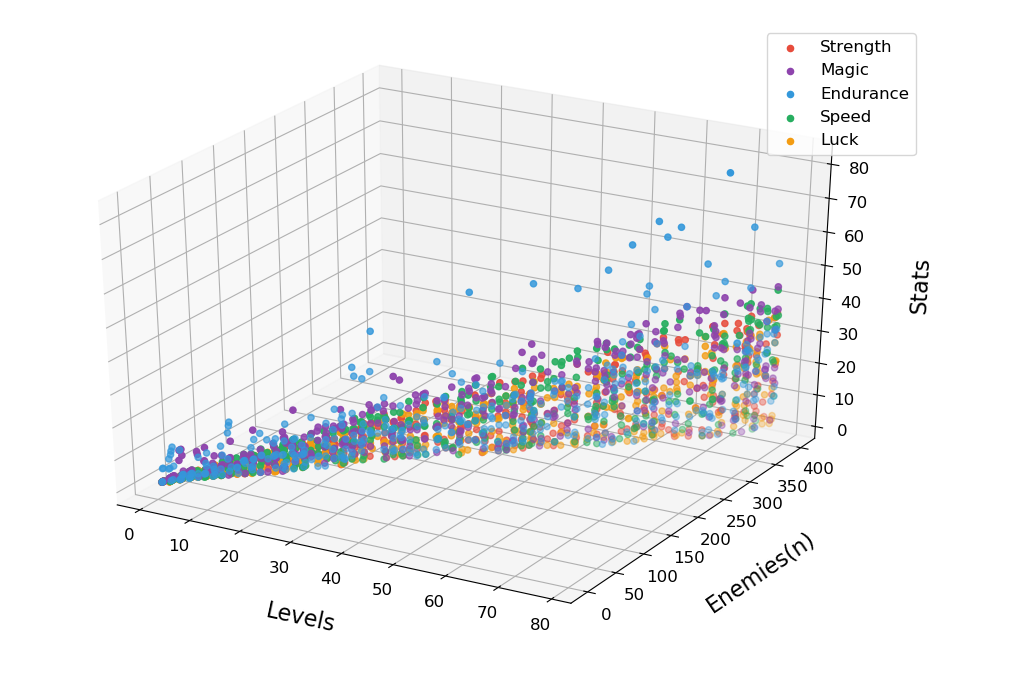
\includegraphics[scale=0.59]{img/EnemyStatsDistrib.png}
	\caption{Distribusi \textit{stats} musuh secara keseluruhan.}
	\label{fig:enemy_all_stats_distrib}
\end{figure}

Selanjutnya adalah penggambaran persebaran \textit{stats} HP dan MP yang masing-masing dijabarkan pada persamaan \ref{fig:enemy_hp_distrib} dan persamaan \ref{fig:enemy_mp_distrib}. Sama seperti pada persamaan \ref{fig:enemy_all_stats_distrib}, yang mana pada persamaan \ref{fig:enemy_hp_distrib} dan persamaan \ref{fig:enemy_mp_distrib} divisualisasikan secara ke dalam bentuk tiga dimensi. Hal tersebut dilakukan agar terciptanya perbandingan antara level, jumlah musuh, dan tingkat tingginya nilai \textit{stats} yang bersangkutan.

\begin{figure} [!h]
\begin{minipage}[t]{1.0\linewidth}
	\centering
	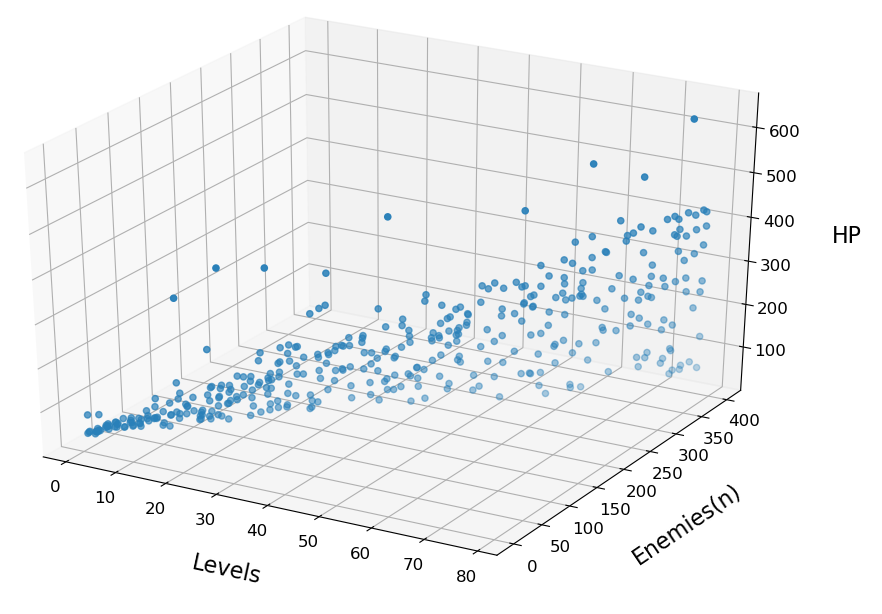
\includegraphics[scale=0.58]{img/EnemyHpDistrib.png}
	\caption{Distribusi \textit{stats} HP musuh.}
	\label{fig:enemy_hp_distrib}
	\vspace{2ex}
\end{minipage}
\vfill
\begin{minipage}[t]{1.0\linewidth}
	\centering
	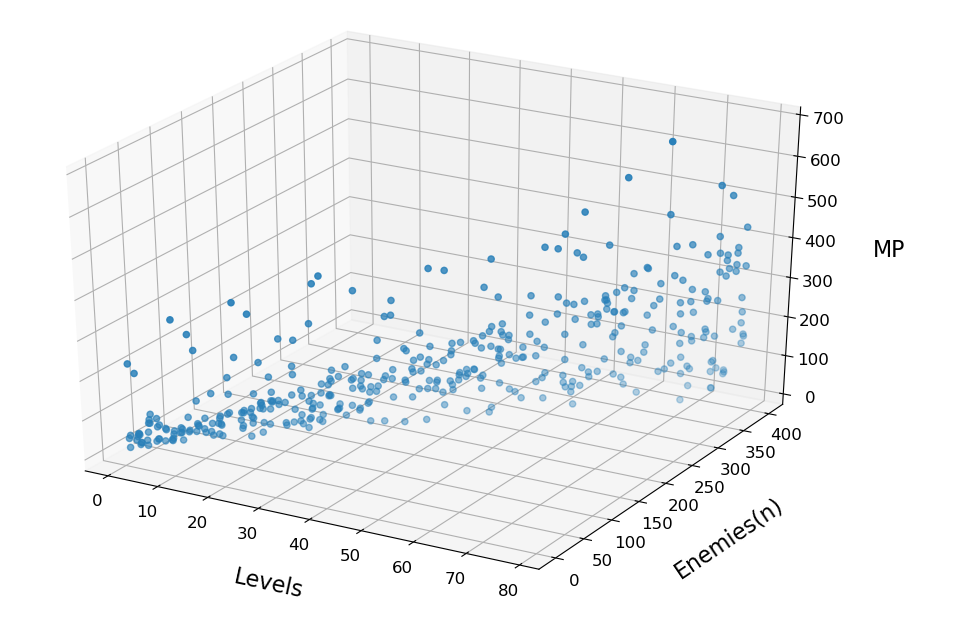
\includegraphics[scale=0.58]{img/EnemyMpDistrib.png}
	\caption{Distribusi \textit{stats} MP musuh.}
	\label{fig:enemy_mp_distrib}
\end{minipage} 
\end{figure}
\vspace{1ex}

Pada Gambar \ref{fig:enemy_str_distrib}, \ref{fig:enemy_mag_distrib}, \ref{fig:enemy_endr_distrib}, \ref{fig:enemy_spd_distrib} dan Gambar \ref{fig:enemy_luck_distrib} adalah pecahan dari Gambar \ref{fig:enemy_all_stats_distrib} secara berurutan diantaranya adalah \textit{Strength}, \textit{Magic}, \textit{Endurance}, \textit{Speed} dan \textit{Luck}.

\begin{figure} [!h]
	\begin{minipage}[t]{1.0\linewidth}
		\centering
		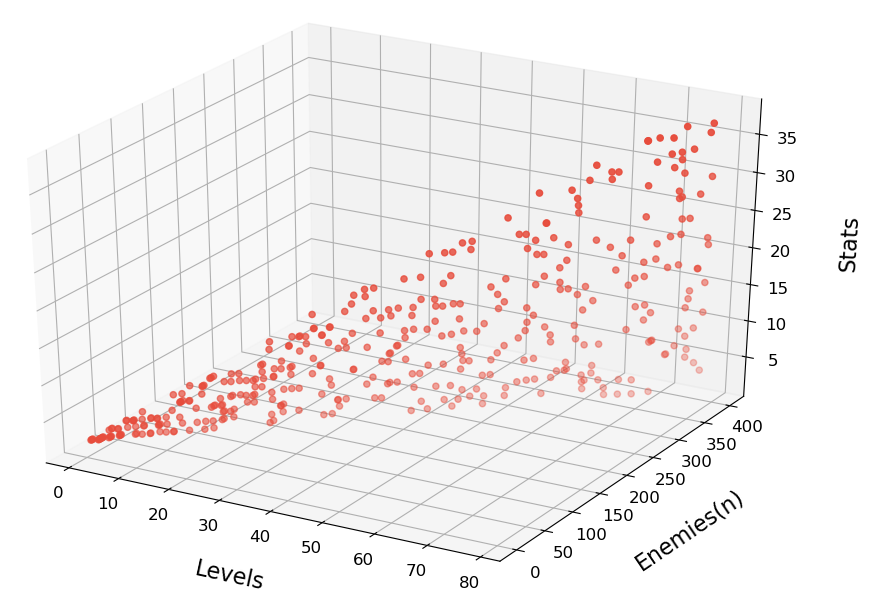
\includegraphics[scale=0.57]{img/EnemyStrengthDistrib.png}
		\caption{Distribusi \textit{Strength} musuh.}
		\label{fig:enemy_str_distrib}
		\vspace{2ex}
	\end{minipage}
	\vfill
	\begin{minipage}[t]{1.0\linewidth}
		\centering
		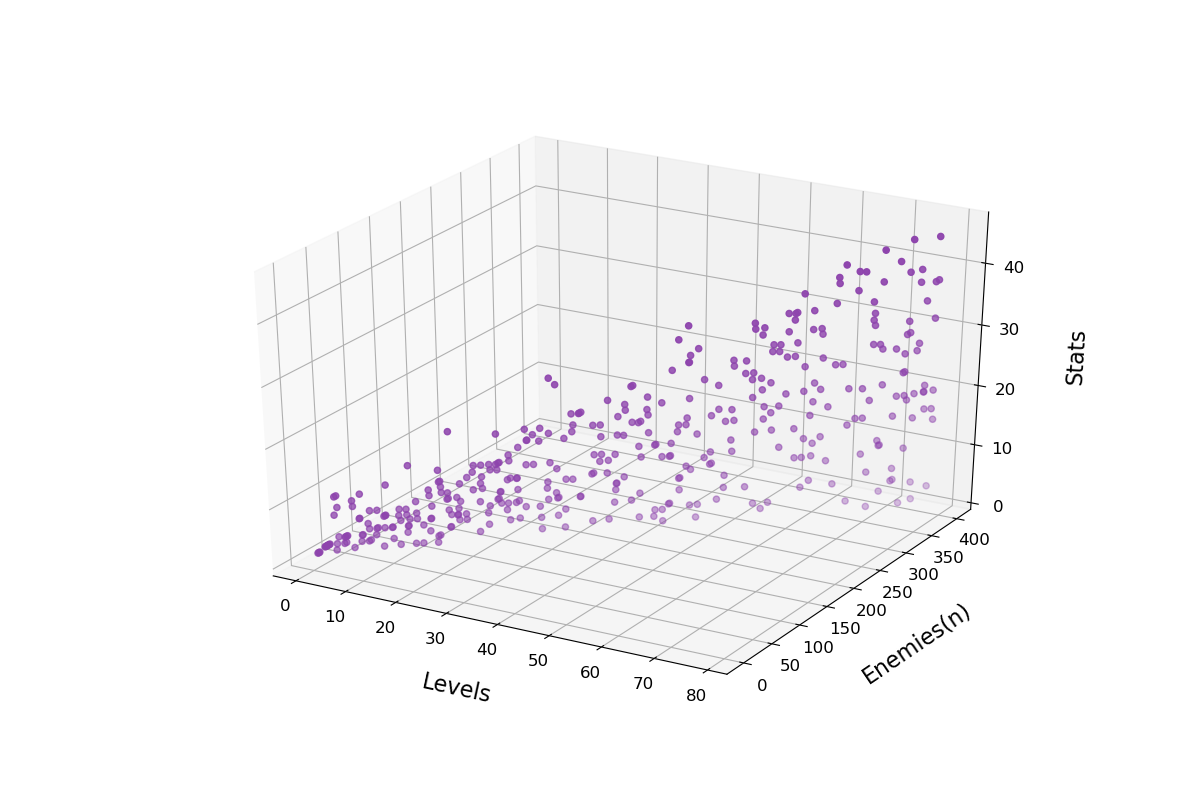
\includegraphics[scale=0.57]{img/EnemyMagicDistrib.png}
		\caption{Distribusi \textit{Magic} musuh.}
		\label{fig:enemy_mag_distrib}
	\end{minipage} 
\end{figure}

\begin{figure} [!h] \centering
	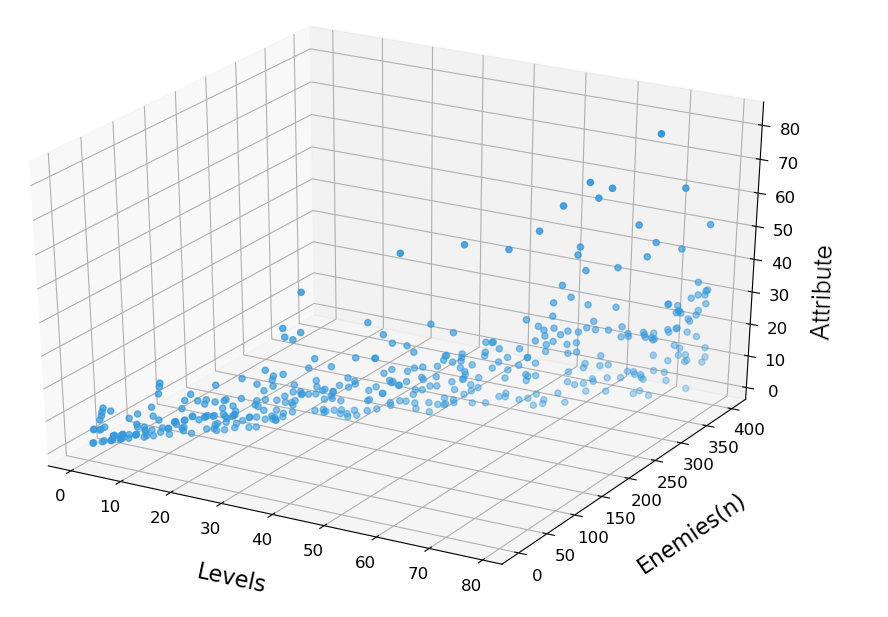
\includegraphics[scale=0.58]{img/EnemyEnduranceDistrib.png}
	\caption{Distribusi \textit{Endurance} musuh.}
	\label{fig:enemy_endr_distrib}
\end{figure}

\begin{figure} [!h] \centering
	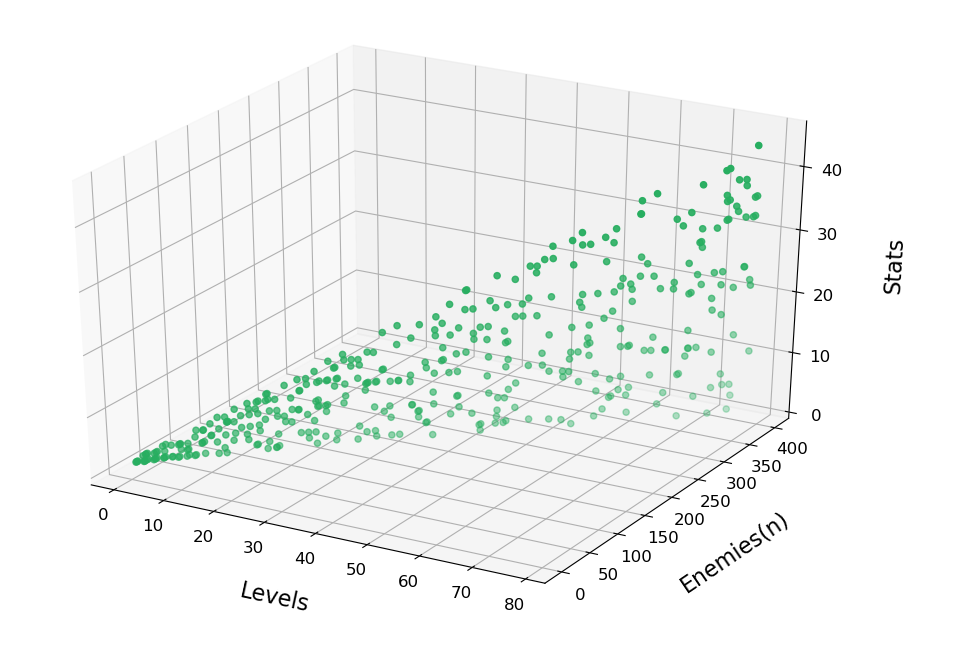
\includegraphics[scale=0.58]{img/EnemySpeedDistrib.png}
	\caption{Distribusi \textit{Speed} musuh.}
	\label{fig:enemy_spd_distrib}
\end{figure}

\begin{figure} [!h] \centering
	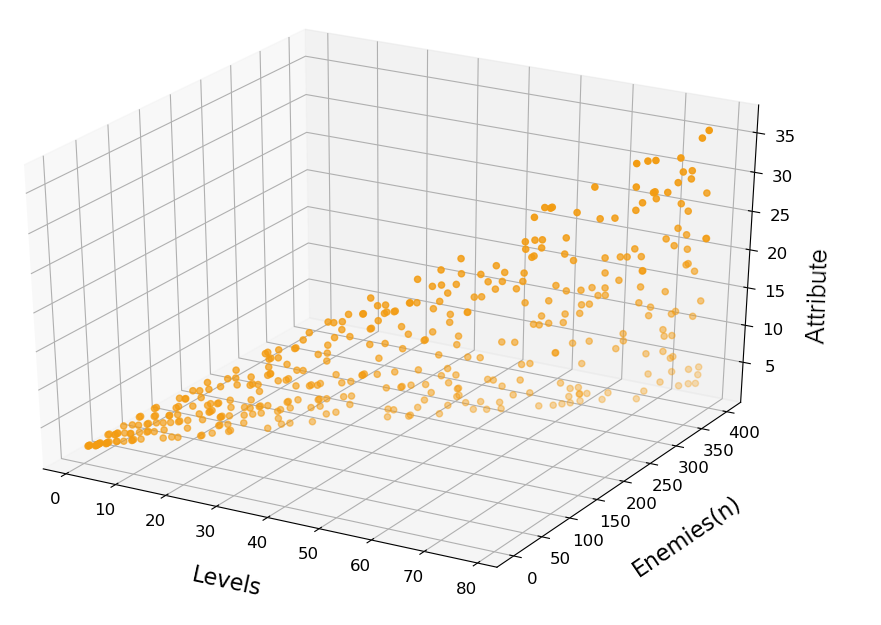
\includegraphics[scale=0.58]{img/EnemyLuckDistrib.png}
	\caption{Distribusi \textit{Luck} musuh.}
	\label{fig:enemy_luck_distrib}
\end{figure}
	\cleardoublepage
	\chapter{PENGUJIAN}
\label{chap:chap4_eval}
\vspace{1ex}


\section*{}
Inti dari BAB \ref{chap:chap4_eval} pada penelitian adalah pengujian dengan berbagai parameter untuk \textit{stats} pemain dan musuh. Seperti halnya \textit{stats} pemain dan musuh pada permainan dengan genre \textit{turn-based} dan \textit{action} RPG.
\vspace{1ex}

\section{Pengujian dalam Pembuatan \textit{Stats} Pemain pada Permainan dengan Genre \textit{Turn-based} RPG}
\label{sec:sec4_eval_turn-based_player}
\vspace{1ex}

Pada bagian ini setiap langkah yang akan diuji sudah dijelaskan pada Sub-bab \ref{sec:sec3_player_stats}, dimana pada bagian ini membahas tentang pembuatan \textit{stats} pemain untuk permaian dengan genre \textit{turn-based} RPG. Melalui berbagai proses seperti yang dijelaskan pada Sub-bab \ref{sec:sec3_player_stats}, maka pada beberapa Sub-bab dibawah ini adalah langkah-langkah dalam proses pengujiannya.
\vspace{1ex}


\subsection{Pengujian Distibusi Level, HP, dan MP Pemain}
\label{sec:sub_sec4_eval_dist_hp_mp_level}
\vspace{1ex}

Seperti yang sudah dijelaskan pada Sub-bab \ref{sec:sub_sec3_enemy_hp_mp_stats}, dimana pada bagian ini membahas tentang pembuatan level, HP dan MP pemain untuk permaian dengan genre \textit{turn-based} RPG. Berikut adalah hasil dari prosess pembuatan Level, HP, dan MP yang dipeeroleh dari perhitungan pada persamaan \ref{eq:hp_player} dan \ref{eq:mp_player} dengan data masukan pada Tabel \ref{tb:player_input_variable} yang kemudian menghasilkan data seperti yang ditunjukkan pada Tabel \ref{tb:player_hp_mp}.

\begin{longtable}{|l|l|l|}
	\caption{Hasil Perhitungan HP dan MP}
	\label{tb:player_hp_mp}\\
	\hline
	\rowcolor[HTML]{C0C0C0} 
	\textbf{Levels} & \textbf{HP} & \textbf{MP} \\ \hline
	1 & 159 & 89 \\ \hline
	2 & 163 & 93 \\ \hline
	3 & 167 & 97 \\ \hline
	4 & 171 & 101 \\ \hline
	5 & 175 & 105 \\ \hline
	6 & 179 & 109 \\ \hline
	7 & 183 & 113 \\ \hline
	... & ... & ... \\ \hline
	\textbf{100} & \textbf{555} & \textbf{485} \\ \hline
\end{longtable}
\vspace{1ex}

Hasil perhitungan tersebut terlihat membentuk pola linier, yang mana nilai HP dan MP terus naik secara konstan ke atas sesuai dengan kenaikan levelnya seperti yang direpresentasikan pada Gambar \ref{fig:hp_player} dan Gambar \ref{fig:mp_player}.

\begin{figure} [!h] \centering
	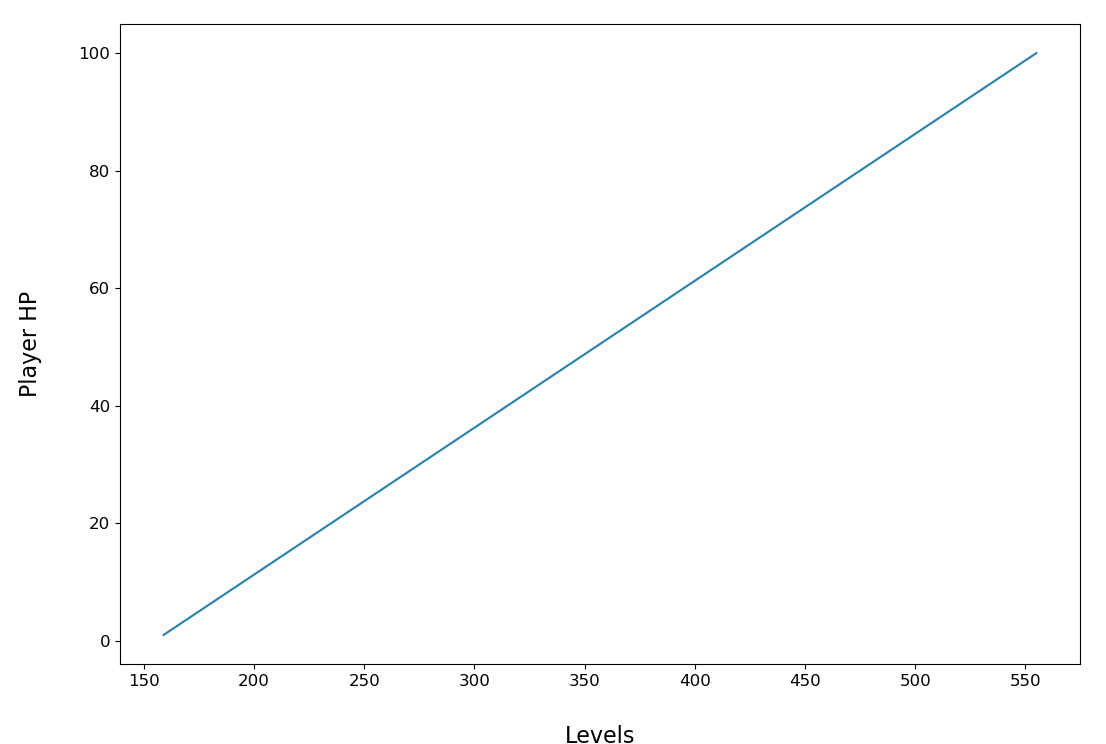
\includegraphics[scale=0.45]{img/PlayerHpDistrib.png}
	\caption{Kenaikan HP setiap levelnya.}
	\label{fig:hp_player}
\end{figure}

Jika melihat Gambar \ref{fig:hp_player} dengan jumlah HP dari pemain yang terus naik mengikuti pola yang dihasilkan pada Tabel \ref{tb:player_hp_mp}, yang mana nilai tersebut diperoleh dari inisiasi variabel pada Tabel \ref{tb:player_input_variable} yaitu \textit{Max Level}, \textit{Start} HP dan \textit{Next} HP. Variabel-variabel tersebut dihitung dengan menggunakan persamaan \ref{eq:hp_player} agar membentuk pola kenaikan HP setiap levelnya seperti yang ditunjukan pada Gambar \ref{fig:hp_player}. Sama seperti pada Gambar \ref{fig:hp_player}, pada Gambar \ref{fig:mp_player} dengan jumlah MP dari pemain yang terus naik mengikuti pola yang dihasilkan pada Tabel \ref{tb:player_hp_mp}, yang mana nilai tersebut diperoleh dari inisiasi variabel pada Tabel \ref{tb:player_input_variable} yaitu \textit{Max Level}, \textit{Start} MP dan \textit{Next} MP. Kemudian variabel-variabel tersebut dihitung dengan menggunakan persamaan \ref{eq:mp_player} agar membentuk pola kenaikan MP setiap levelnya seperti yang ditunjukan pada Gambar \ref{fig:mp_player}.

\begin{figure} [!h] \centering
	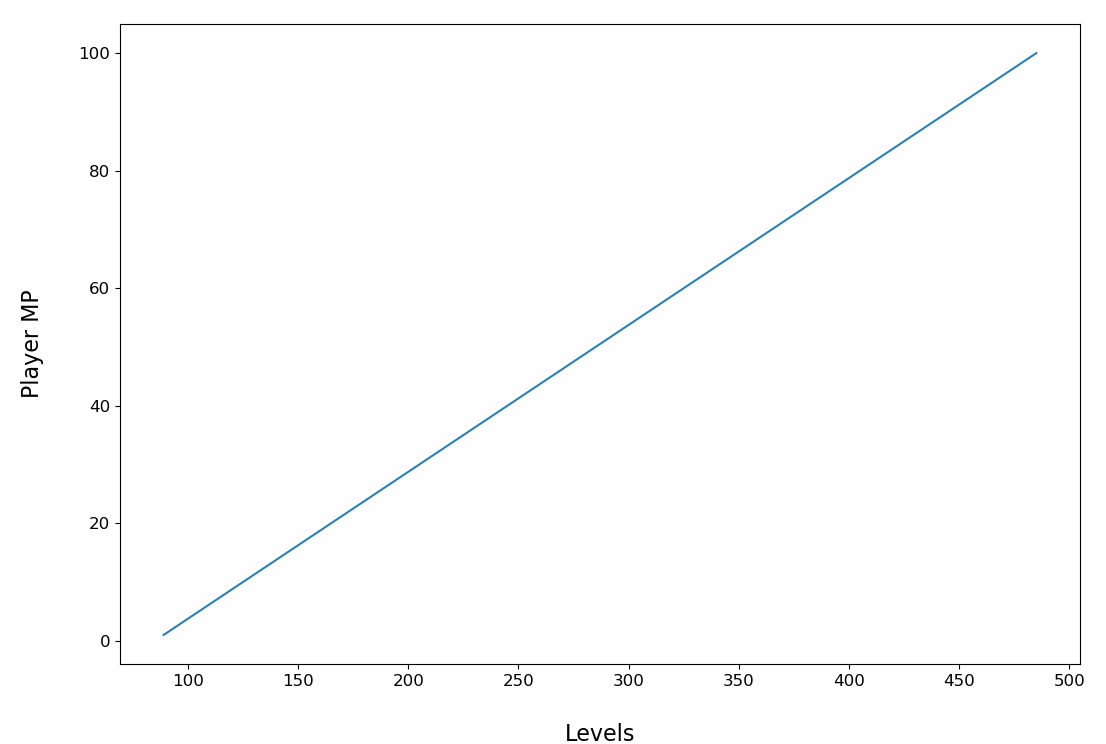
\includegraphics[scale=0.45]{img/PlayerMpDistrib.png}
	\caption{Kenaikan MP setiap levelnya.}
	\label{fig:mp_player}
\end{figure}
\vspace{1ex}


\subsection{Pengujian Distibusi Stats Pemain}
\label{sec:sub_sec4_eval_player_stats}
\vspace{1ex}

Pada bagian ini setiap langkah yang akan diuji sudah dijelaskan pada Sub-bab \ref{sec:sub_sec3_stat_pemain}, dimana pada bagian ini membahas tentang pembuatan \textit{stats} pemain untuk permaian dengan genre \textit{turn-based} RPG. Melalui berbagai proses seperti yang dijelaskan pada Sub-bab \ref{sec:sub_sec3_stat_pemain}, melalui persamaan \ref{eq:KNN_bayes_player_stats} dan beberapa persamaan yang digunakan sebelumnya pada Sub-bab \ref{sec:sub_sec3_stat_pemain} dihasilkan data seperti yang ditunjukan pada Tabel \ref{tb:player_battle_stats}, dan bila divisualisasikan hasilnya akan tampak seperti pada Gambar \ref{fig:stats_player}.
\vspace{-1ex}

\begin{longtable}{|l|l|l|l|l|l|}
	\caption{Sampel hasil perhitungan dan distribusi stats dengan $k-$NN}
	\label{tb:player_battle_stats}\\
	\hline
	\rowcolor[HTML]{C0C0C0} 
	\textbf{Levels} & \textbf{Strength} & \textbf{Magic} & \textbf{Endurance} & \textbf{Speed} & \textbf{Luck} \\ \hline
	1 & 1 & 2 & 0 & 0 & 1 \\ \hline
	2 & 0 & 2 & 0 & 2 & 0 \\ \hline
	3 & 1 & 0 & 0 & 0 & 0 \\ \hline
	4 & 1 & 1 & 0 & 0 & 0 \\ \hline
	5 & 1 & 1 & 0 & 0 & 0 \\ \hline
	6 & 1 & 1 & 0 & 2 & 1 \\ \hline
	7 & 0 & 0 & 0 & 0 & 1 \\ \hline
	8 & 1 & 0 & 0 & 0 & 0 \\ \hline
	... & ... & ... & ... & ... & ... \\ \hline
	\textbf{100} & \textbf{1} & \textbf{0} & \textbf{0} & \textbf{0} & \textbf{0} \\ \hline
\end{longtable}

\begin{figure} [!h] \centering
	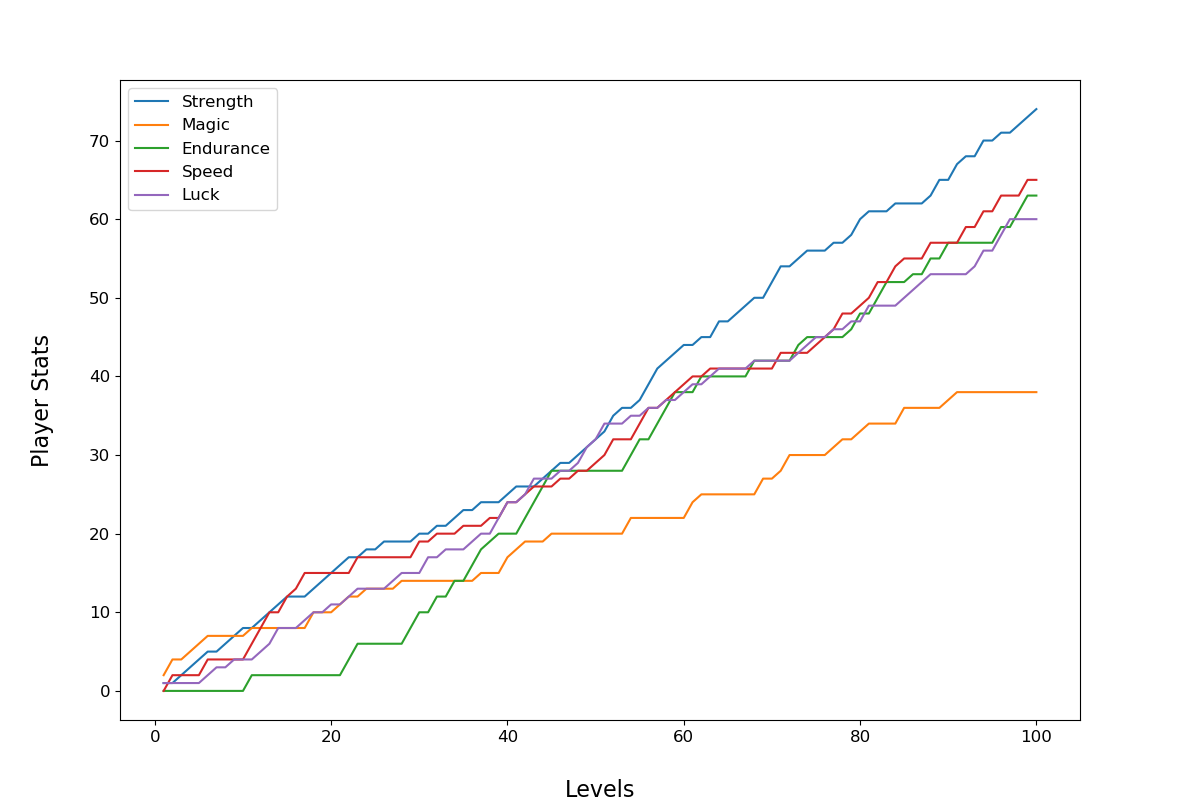
\includegraphics[scale=0.50]{img/PlayerStatsDistrib.png}
	\caption{Kenaikan stats pemain setiap levelnya.}
	\label{fig:stats_player}
\end{figure}

Pada Tabel \ref{tb:player_battle_stats} adalah data \textit{stats} dari pemain yang dihasilakn melalui penambahan nilai pada \textit{stats} secara acak pada setiap \textit{stats}. Seperti yang dijelaskan pada persaamaan \ref{eq:nbayes_class}, \ref{eq:KNN_distance_stats}, dan persamaan \ref{eq:KNN_bayes_player_stats} saat nilai \textit{stats} di tambahkan secara acak dari 1 sampai dengan 2 pada level yang berjarak antara 1 sampai dengan 100. Selanjutnya representasi dari hasil penambahan \textit{stats} tersebut yang ditunjukan melalui Gambar \ref{fig:stats_player} yang mana nilai dari setiap \textit{stats} terus naik sesuai dengan level pemain yang juga terus naik. 
\vspace{1ex}


\section{Pengujian dalam Pembuatan \textit{Stats} Musuh pada Permainan dengan Genre \textit{Turn-based} RPG}
\label{sec:sec4_eval_turn-based_enemy}
\vspace{1ex}

Pada bagian ini setiap langkah yang akan diuji sudah dijelaskan pada Bagian \ref{sec:sec3_enemy_stats}, dimana pada bagian ini membahas tentang pembuatan \textit{stats} musuh untuk permaian dengan genre \textit{turn-based} RPG. Melalui berbagai proses seperti yang dijelaskan pada Bagian \ref{sec:sec3_player_stats}, maka pada beberapa Sub-bab dibawah ini adalah langkah-langkah dalam proses pengujiannya.
\vspace{1ex}


\subsection{Pengujian Distibusi Level Musuh}
\label{sec:sub_sec4_eval_dist_enemy_level}
\vspace{1ex}

Seperti yang sudah dijelaskan pada Sub-bab \ref{sec:sub_sec3_enemy_level}, dimana pada bagian ini membahas tentang pendistribusian level musuh untuk permaian dengan genre \textit{turn-based} RPG. Berikut adalah hasil dari proses distribusi level yang diperoleh dari perhitungan pada persamaan \ref{eq:enemy_levels1}, \ref{eq:enemy_levels2}, \ref{eq:sub_enemy_levels1}, \ref{eq:sub_enemy_levels2} dan persamaan \ref{eq:probability_enemy_levels}. Setelah melalui tahapan tersebut dan dengan variabel masukan pada Tabel \ref{tb:enemy_input_variable} maka level yang dihasilkan akan seperti pada Tabel \ref{tb:enemy_level_distrib}.

\begin{longtable}{|l|l|l|}
	\caption{Hasil level yang dibuat untuk musuh.}
	\label{tb:enemy_level_distrib}\\
	\hline
	\rowcolor[HTML]{C0C0C0} 
	\textbf{No.} & \textbf{Name} & \textbf{Levels} \\ \hline
	1 & Enemy 1 & 1 \\ \hline
	2 & Enemy 2 & 1 \\ \hline
	3 & Enemy 3 & 1 \\ \hline
	4 & Enemy 4 & 1 \\ \hline
	5 & Enemy 5 & 2 \\ \hline
	6 & Enemy 6 & 2 \\ \hline
	7 & Enemy 7 & 2 \\ \hline
	8 & Enemy 8 & 2 \\ \hline
	9 & Enemy 9 & 2 \\ \hline
	10 & Enemy 10 & 2 \\ \hline
	11 & Enemy 11 & 2 \\ \hline
	12 & Enemy 12 & 2 \\ \hline
	13 & Enemy 13 & 2 \\ \hline
	14 & Enemy 14 & 3 \\ \hline
	15 & Enemy 15 & 3 \\ \hline
	... & ... & ... \\ \hline
	\textbf{400} & \textbf{Enemy 400} & \textbf{78} \\ \hline
\end{longtable}

Pada Tabel \ref{tb:enemy_level_distrib} adalah sebagian data dari level yang dihasilkan oleh program, untuk hasil lebih lengkapnya bisa dilihat pada Bagian \nameref{chap:chap6_attachment} pada Tabel \ref{tb:enemies_all_stats_1} sampai dengan Tabel \ref{tb:enemies_all_stats_15} di kolom \textit{Levels}. Kemudian persebaran level yang dihasilkan tersebut bila divisualisasikan maka hasilnya akan seperti yang ditujukkkan pada Gambar \ref{fig:enemy_level_distrib}. Grafik atau histogram yang ditunjukan pada Gambar \ref{fig:enemy_level_distrib} tersebut sangatlah tidak merata, hal tersebut dikarenakan proses penentuan level yang ditentukan secara acak.

\begin{figure} [!h] \centering
	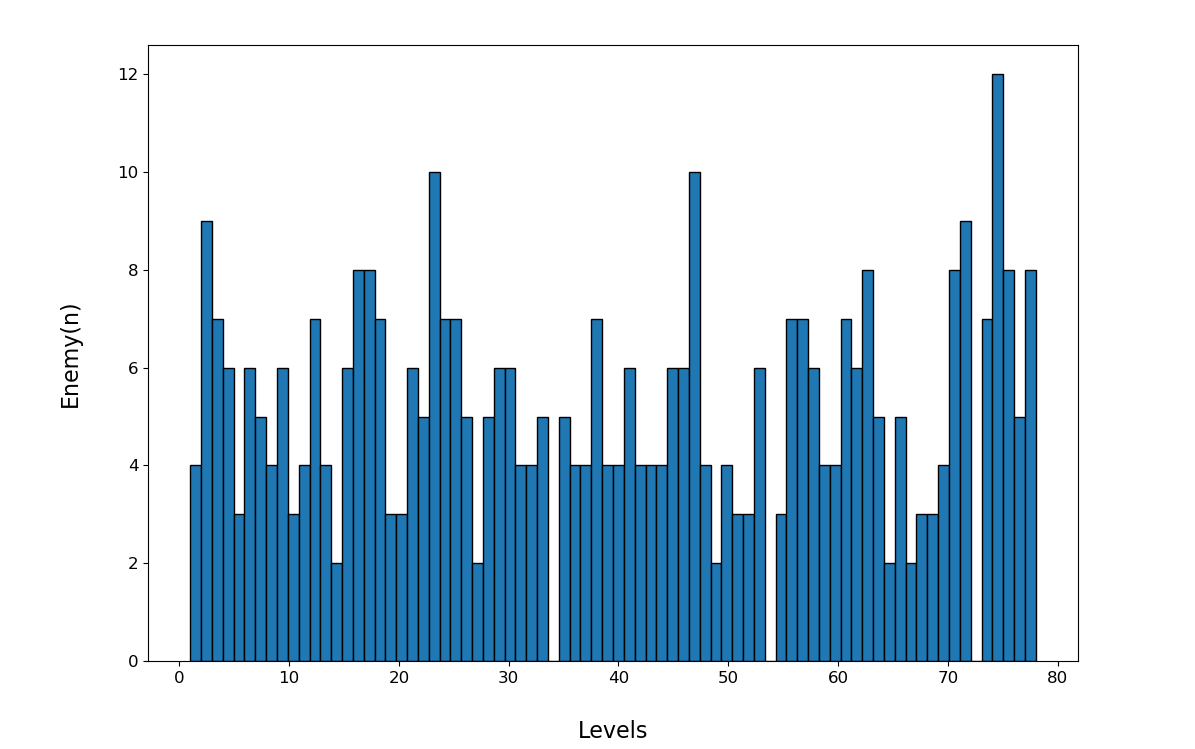
\includegraphics[scale=0.48]{img/EnemyLevelDistrib.png}
	\caption{Distribusi Level Musuh.}
	\label{fig:enemy_level_distrib}
\end{figure}

Dilanjutkan dengan validasi dari keseimbangan persebaran level musuh, hal ini dilakukan dengan menggunakkan persamaan melalui beberapa langkah seperti yang ditunjukan oleh persamaan \ref{eq:mean_enemy_levels}, \ref{eq:varian_enemy_levels}, \ref{eq:stdev_enemy_levels} dan persamaan \ref{eq:PDF_enemy_levels}. Konsep tersebut beracuan pada Sub-bab \ref{sec:sub_sec2_gauss_bayes} tentang \textit{Gaussian Naive bayes}, dengan harapan apakah setiap data yang dihasilkan sebelumnya sudah terdistribusi dengan normal atau tidak. Jika memang benar data hasil program ini valid maka ketika musuh bertambah maka pola dari level dan jumlah musuh masih akan membentuk pola distribusi normal seperti pada Gambar \ref{fig:enemy_level_distrib_ndist}.

\begin{figure} [!h] \centering
	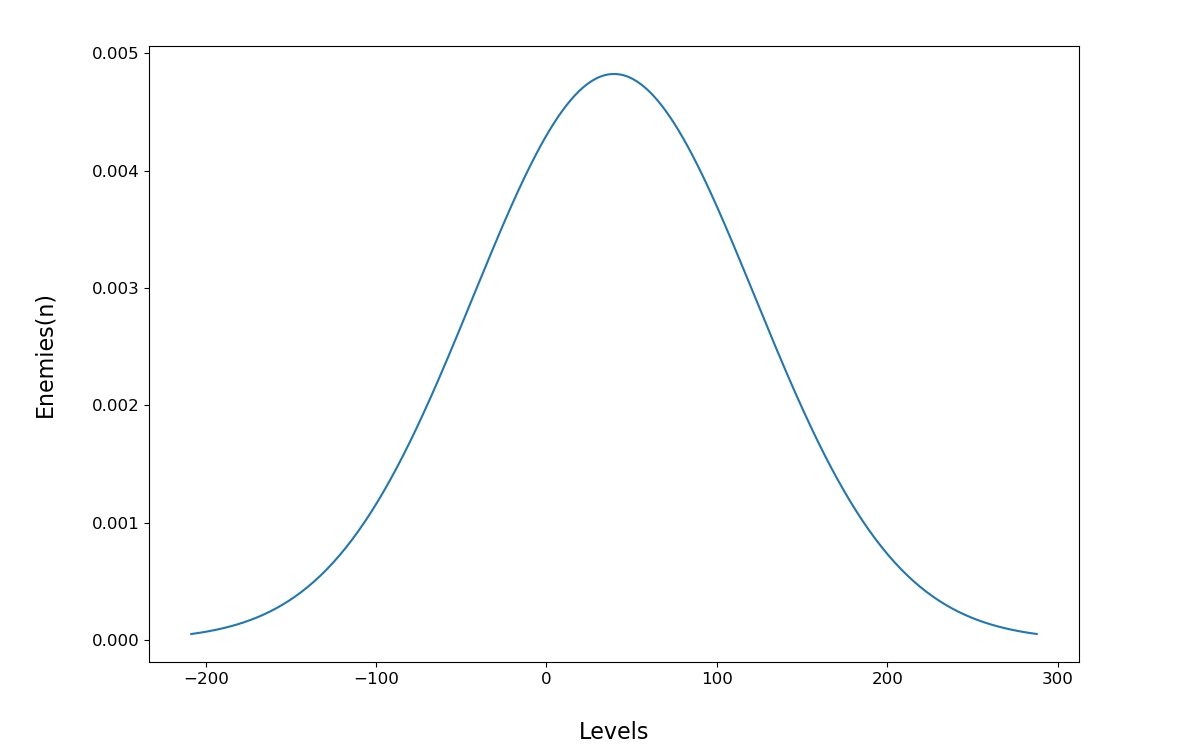
\includegraphics[scale=0.45]{img/EnemyLevelDistribNdist.png}
	\caption{Distribusi level musuh dalam bentuk distribusi normal.}
	\label{fig:enemy_level_distrib_ndist}
\end{figure}

Pada Gambar \ref{fig:enemy_level_distrib_ndist} jika dilihat persebaran datanya dari kiri ke kanan menggambarkan tingkat kesulitan musuh berdasarkan level, jumlah musuh pada sisi kiri berjumlah sedikit semakin ke kanan jumlahnya meningkat dan semakin ke kanan jumlah musuh kembali menjadi sedikit jumlahnya. Hal tersebut menggambarkan tingkat keseimbangan dari musuh yang dibuat, yang mana jumlah musuh dengan level menengah berjumlah paling banyak dan jumlah musuh yang sangat sulit dan sangat mudah dikalahkan berjummlah sedikit. Tujuan utama dari kondisi tersebut adalah terjadinya keseimbangan saat terjadinya pertarungan antara pemain dan musuh.
\vspace{1ex}


\subsection{Pengujian Distibusi Type Musuh}
\label{sec:sub_sec4_eval_dist_enemy_type}
\vspace{1ex}

Seperti yang sudah dijelaskan pada Sub-bab \ref{sec:sub_sec3_enemy_type}, dimana pada bagian ini membahas tentang pendistribusian tipe musuh untuk permaian dengan genre \textit{turn-based} RPG. Berikut adalah hasil dari proses distribusi tipe musuh yang diperoleh dari perhitungan pada persamaan \ref{eq:enemy_types_percentage}, \ref{eq:enemy_types_dist_level}, \ref{eq:enemy_types_rest_dist_level}, \ref{eq:enemy_types_probability}, \ref{eq:enemy_rest_types} dan persamaan \ref{eq:enemy_types_rest_probability}. Setelah melalui tahapan tersebut dengan variabel masukan pada Tabel \ref{tb:enemy_input_variable} maka hasil distribusi dan penjelasan level yang dilakukan oleh beberapa persamaan tersebut akan menjadi seperti Tabel \ref{tb:enemy_type_distrib}.

\begin{longtable}{|l|l|l|l|}
	\caption{Hasil level yang dibuat untuk musuh.}
	\label{tb:enemy_type_distrib}\\
	\hline
	\rowcolor[HTML]{C0C0C0} 
	\textbf{No.} & \textbf{Name} & \textbf{Levels} & \textbf{Type} \\ \hline
	1 & Enemy 1 & 1 & 0 \\ \hline
	2 & Enemy 2 & 1 & 0 \\ \hline
	3 & Enemy 3 & 1 & 2 \\ \hline
	4 & Enemy 4 & 1 & 1 \\ \hline
	5 & Enemy 5 & 2 & 2 \\ \hline
	6 & Enemy 6 & 2 & 1 \\ \hline
	7 & Enemy 7 & 2 & 2 \\ \hline
	8 & Enemy 8 & 2 & 0 \\ \hline
	9 & Enemy 9 & 2 & 2 \\ \hline
	10 & Enemy 10 & 2 & 2 \\ \hline
	11 & Enemy 11 & 2 & 4 \\ \hline
	12 & Enemy 12 & 2 & 0 \\ \hline
	13 & Enemy 13 & 2 & 0 \\ \hline
	14 & Enemy 14 & 3 & 4 \\ \hline
	15 & Enemy 15 & 3 & 4 \\ \hline
	16 & Enemy 16 & 3 & 2 \\ \hline
	... & ... & ... & ... \\ \hline
	\textbf{400} & \textbf{Enemy 400} & \textbf{78} & \textbf{3} \\ \hline
\end{longtable}

Dari data yang tedapat pada Tabel \ref{tb:enemy_type_distrib} hanya sebagian data saja, lebih lengkapnya dapat dilihat langsung pada Bagian \nameref{chap:chap6_attachment} dalam Tabel \ref{tb:enemies_all_stats_1} sampai dengan Tabel \ref{tb:enemies_all_stats_15} di kolom \textit{Type}. Pada Tabel \ref{tb:enemy_type_distrib} dan tabel lain yang memuat tentang \textit{Type} yang berisi data $ET_{i}$ atau jenis musuh yang diisi dengan angka 0 sampai dengan 4, maksud dari angka tersebut adalah untuk mewakili indeks dari variabel \textit{Enemy Type} pada Tabel \ref{tb:enemy_input_variable}. Secara berurutan dari 0 sampai dengan 4 adalah \textit{Mixed}, \textit{Hard Magic}, \textit{Soft Magic}, \textit{Hard Strength}, dan \textit{Soft Magic}. Seluruh data tersebut jika divisualisasikan maka hasilnya seperti Gambar \ref{fig:enemy_type_distrib} sesuai yang ditargetkan oleh variabel \textit{Distribute Percentage} pada Tabel \ref{tb:enemy_input_variable} atau variabel $DP$ pada persamaan \ref{eq:enemy_types_percentage}.

\begin{figure} [!h] \centering
	\includegraphics[scale=0.48]{img/EnemyTypeDistrib.png}
	\caption{Distribusi tipe musuh.}
	\label{fig:enemy_type_distrib}
\end{figure}

Kemudian pada Gambar \ref{fig:enemy_type_distrib} adalah hasil dari proses pembuatan dan pengelompokan musuh berdasarkan tipe yang sudah sesuai dengan variabel masukan pada Tabel \ref{tb:enemy_input_variable}. Dengan musuh bertipe \textit{Mixed} berjumlah yang paling banyak, diikuti \textit{soft magic} dan \textit{soft strength} dengan harapan bahwa ini adalah musuh yang memiliki karakter \textit{magic} dan \textit{strength} namun masih mudah dikalahkan, dilanjutkan dengan yang paling sedikit adalah \textit{hard magic} dan \textit{hard strength} dengan harapan menjadi musuh berkarakter strength dan magic yang sulit dikalahkan.
\vspace{1ex}


\subsection{Pengujian Distribusi Element dan Kelemahan pada Musuh}
\label{sec:sub_sec4_eval_dist_enemy_element_and_weak}
\vspace{1ex}

Seperti yang sudah dijelaskan pada Sub-bab \ref{sec:sub_sec3_enemy_weak}, dimana pada bagian ini membahas tentang pendistribusian elemen dan kelemahan musuh untuk permaian dengan genre \textit{turn-based} RPG. Berikut adalah hasil dari proses distribusi tipe musuh yang diperoleh dari perhitungan pada persamaan \ref{eq:enemy_element}, \ref{eq:damage_name_number}, \ref{eq:damage_number_prob}, \ref{eq:multi_damage_num_prob}, dan \ref{eq:all_enemies_damage}. Setelah melalui tahapan tersebut dengan variabel masukan pada Tabel \ref{tb:enemy_input_variable} maka hasil persebaran kelemahan dan kekebalan musuh ditunjukkan pada Tabel \ref{tb:enemy_weak_distrib}.

\begin{longtable}{|l|l|l|l|l|l|l|}
	\caption{Hasil level yang dibuat untuk musuh.}
	\label{tb:enemy_weak_distrib}\\
	\hline
	\rowcolor[HTML]{C0C0C0} 
	\textbf{No.} & \textbf{Name} & \textbf{Phys} & \textbf{Water} & \textbf{Wind} & \textbf{Earth} & \textbf{Fire} \\ \hline
	1 & Enemy 1 & 1 & 1 & 0 & 1 & 0 \\ \hline
	2 & Enemy 2 & 0 & 0 & 0 & 0 & 0 \\ \hline
	3 & Enemy 3 & 0 & 1 & 0 & 1 & 1 \\ \hline
	4 & Enemy 4 & 1 & 0 & 1 & 0 & 0 \\ \hline
	5 & Enemy 5 & 0 & 1 & 0 & 0 & 1 \\ \hline
	6 & Enemy 6 & 1 & 1 & 0 & 1 & 0 \\ \hline
	7 & Enemy 7 & 1 & 0 & 0 & 0 & 0 \\ \hline
	8 & Enemy 8 & 0 & 0 & 0 & 0 & 1 \\ \hline
	9 & Enemy 9 & 1 & 1 & 0 & 0 & 0 \\ \hline
	10 & Enemy 10 & 0 & 0 & 0 & 0 & 0 \\ \hline
	11 & Enemy 11 & 1 & 0 & 0 & 1 & 0 \\ \hline
	12 & Enemy 12 & 0 & 0 & 0 & 0 & 1 \\ \hline
	13 & Enemy 13 & 0 & 0 & 2 & 1 & 0 \\ \hline
	%14 & Enemy 14 & 0 & 1 & 0 & 0 & 0 \\ \hline
	... & ... & ... & ... & ... & ... & ... \\ \hline
	\textbf{400} & \textbf{Enemy 400} & \textbf{0} & \textbf{0} & \textbf{2} & \textbf{1} & \textbf{0} \\ \hline
\end{longtable}
\vspace{1ex}

Jika melihat Tabel \ref{tb:enemy_weak_distrib} dengan melihat pada kolom \textit{Phys}, \textit{Water}, \textit{Wind}, \textit{Earth}, dan \textit{Fire}, isi dari kolom tersebut berupa angka nol sampai dengan dua adalah hasil dari pembuatan \textit{stats} kelemahan musuh pada variabel $DmgEN_{M}$ atau untuk $DmgEN_{M} = \left \{ DmgNu_{0}, DmgNu_{1}, DmgNu_{2},..., DmgNu_{M} \right \}$ jika jumlah kelemahan musuh lebih dari tiga atau yang dicontohkan pada Tabel \ref{tb:enemy_input_variable} dalam variabel \textit{List Damage}. Hasil dari proses yang sebelumnya dijelaskan pada Sub-bab ini menghasilkan persebaran kelemahan dan kekebalan musuh yang ditunjukkan pada Gambar \ref{fig:enemy_weak_distrib} dibawah ini.

\begin{figure} [!h] \centering
	\includegraphics[scale=0.50]{img/EnemyWeakDistrib.png}
	\caption{Distribusi kelemahan musuh.}
	\label{fig:enemy_weak_distrib}
\end{figure}

Pada Gambar \ref{fig:enemy_weak_distrib} dapat dilihat distribusi musuh dengan kelemahan dan kekebalannya. Terlihat pada kondisi tersebut jumlah musuh dengan kondisi \textit{Normal} memiliki nilai paling tunggi pada setiap kelemahan, hal tersebut dapat diartikan bahwa sebagian besar elemen dari musuh dapat memperoleh \textit{damage} secara normal jika diserang. Kemudian jumlah musuh pada kondisi \textit{Repel} berjumlah terbanyak kedua, hal tersebut dapat diartikan musuh memmiliki jumlah kekebalan terhadap serangan sejumlah angka pada setiap elemen pada Gambar \ref{fig:enemy_weak_distrib}. Begitu juga dengan kondisi \textit{Weaknesses} dengan jumlah paling sedikit, hal tersebut bertujuan agar menjadikan pertarungan antara pemain dan musuh menjadi tidak mudah dimenangkan oleh pemain. Tidak hanya dengan efek \textit{Weaknesses}, efek \textit{Repel} juga sangat berpengaruh dalam menjadikan permainan seperti layaknya sebuah \textit{puzzle} atau teka-teki.
\vspace{1ex}

Sedangkan pada persamaan \ref{eq:multi_damage_num_prob} adalah penjelasan tentang proses munculnya setiap $DmgNu$ pada satu karakter musuh, sehingga variabel tersebut berubah menjadi $DmgNu_{i}$. Seperti penjelasan sebelumnya bahwa pada sebuah karakter musuh dapat memiliki lebih dari satu kelemahan atau kekebalan $DmgNu$ terhadap $DmgNa$ yang diset secara acak seperti yang sudah dijelaskan pada bagian sebelumnya. 
\vspace{1ex}


\subsection{Pengujian Distribusi HP, MP, dan Stats Musuh}
\label{sec:sub_sec4_eval_dist_enemy_HP_MP_Stats}
\vspace{1ex}

pada Sub-bab \ref{sec:sub_sec3_enemy_hp_mp_stats}, dimana pada bagian ini membahas tentang pendistribusian HP dan MP musuh untuk permaian dengan genre \textit{turn-based} RPG. Berikut adalah hasil dari proses distribusi tipe musuh yang diperoleh dari perhitungan pada persamaan \ref{eq:enemy_types_stats_ex} sampai dengan persamaan \ref{eq:enemy_types_prob_hp_mix}, yang mana pada persamaan \ref{eq:enemy_types_stats_ex} sampai dengan persamaan \ref{eq:enemy_types_prob_adv} adalah penenentuan tipe musuh. Setelah melalui tahapan tersebut dengan variabel masukan pada Tabel \ref{tb:enemy_input_variable} maka hasil persebaran kelemahan dan kekebalan musuh ditunjukkan pada Tabel \ref{tb:enemy_weak_distrib}.
\vspace{-1ex}

\begin{longtable}{|l|l|l|l|l|}
	\caption{Distribusi \textit{Stats} HP dan MP musuh.}
	\label{tb:enemy_weak_stats}\\
	\hline
	\rowcolor[HTML]{C0C0C0} 
	\textbf{No.} & \textbf{Name} & \textbf{Levels} & \textbf{HP} & \textbf{MP} \\ \hline
	1 & Enemy 1 & 1 & 42 & 45 \\ \hline
	2 & Enemy 2 & 1 & 84 & 21 \\ \hline
	3 & Enemy 3 & 1 & 43 & 51 \\ \hline
	4 & Enemy 4 & 1 & 44 & 231 \\ \hline
	5 & Enemy 5 & 2 & 40 & 40 \\ \hline
	6 & Enemy 6 & 2 & 44 & 208 \\ \hline
	7 & Enemy 7 & 2 & 44 & 47 \\ \hline
	8 & Enemy 8 & 2 & 42 & 53 \\ \hline
	9 & Enemy 9 & 2 & 49 & 53 \\ \hline
	10 & Enemy 10 & 2 & 42 & 49 \\ \hline
	11 & Enemy 11 & 2 & 44 & 23 \\ \hline
	12 & Enemy 12 & 2 & 79 & 27 \\ \hline
	13 & Enemy 13 & 2 & 41 & 26 \\ \hline
	14 & Enemy 14 & 3 & 50 & 34 \\ \hline
	15 & Enemy 15 & 3 & 54 & 20 \\ \hline
	... & ... & ... & ... & ... \\ \hline
	\textbf{400} & \textbf{Enemy 400} & \textbf{78} & \textbf{389} & \textbf{161} \\ \hline
\end{longtable}
\vspace{1ex}

Pada Tabel \ref{tb:enemy_weak_stats} hanya sebagian data saja yang ditampilkan, untuk selengkapnya dapat dilihat pada Tabel \ref{tb:enemies_all_stats_1} sampai dengan Tabel \ref{tb:enemies_all_stats_15} pada kolom HP dan MP. Selanjutnya adalah penggambaran persebaran \textit{stats} HP dan MP yang masing-masing digambarkan pada Gambar \ref{fig:enemy_hp_distrib} dan Gambar \ref{fig:enemy_mp_distrib}.
\vspace{1ex}

\begin{figure} [!h] \centering
	\centering
	\includegraphics[scale=0.57]{img/EnemyHpDistrib.png}
	\caption{Distribusi \textit{stats} HP musuh.}
	\label{fig:enemy_hp_distrib}
\end{figure}

\begin{figure} [!h] \centering
	\centering
	\includegraphics[scale=0.57]{img/EnemyMpDistrib.png}
	\caption{Distribusi \textit{stats} MP musuh.}
	\label{fig:enemy_mp_distrib}
\end{figure}

Masih pada Sub-bab \ref{sec:sub_sec3_enemy_hp_mp_stats}, dimana pada bagian ini membahas tentang pendistribusian \textit{stats} musuh untuk permaian dengan genre \textit{turn-based} RPG. Berikut adalah hasil dari proses distribusi tipe musuh yang diperoleh dari perhitungan mulai dari persamaan \ref{eq:enemy_types_stats_ex} secara berurutan sampai dengan persamaan \ref{eq:enemy_types_prob_adv} yang digunakan untuk penentuan tipe musuh yang ingin dipakai. Sedangkan proses kalkulasi untuk menentukan \textit{stats} musuh dimulai dari persamaan \ref{eq:enemy_types_prob_bst1} sampai dengan persamaan \ref{eq:enemy_types_prob_st}. Setelah melalui tahapan tersebut dengan variabel masukan pada Tabel \ref{tb:enemy_input_variable} maka hasil persebaran \textit{stats} musuh dengan komposisi \textit{Strength}, \textit{Magic}, \textit{Endurance}, \textit{Speed}, dan \textit{Luck} ditunjukkan pada Tabel \ref{tb:enemy_stats}.
\vspace{-1ex}

\begin{longtable}{|l|l|l|l|l|l|l|l|}
	\caption{Distribusi \textit{Stats} musuh.}
	\label{tb:enemy_stats}\\
	\hline
	\rowcolor[HTML]{C0C0C0} 
	\textbf{No.} & \textbf{Name} & \textbf{Lv.} & \textbf{Str} & \textbf{Mag} & \textbf{Endr} & \textbf{Spd} & \textbf{Luck} \\ \hline
	1 & Enemy 1 & 1 & 2 & 2 & 2 & 2 & 2 \\ \hline
	2 & Enemy 2 & 1 & 2 & 2 & 2 & 2 & 2 \\ \hline
	3 & Enemy 3 & 1 & 2 & 2 & 6 & 2 & 2 \\ \hline
	4 & Enemy 4 & 1 & 2 & 2 & 6 & 2 & 2 \\ \hline
	5 & Enemy 5 & 2 & 2 & 3 & 6 & 3 & 2 \\ \hline
	6 & Enemy 6 & 2 & 2 & 3 & 9 & 2 & 2 \\ \hline
	7 & Enemy 7 & 2 & 2 & 3 & 6 & 2 & 2 \\ \hline
	8 & Enemy 8 & 2 & 2 & 3 & 2 & 2 & 2 \\ \hline
	9 & Enemy 9 & 2 & 2 & 3 & 10 & 3 & 2 \\ \hline
	10 & Enemy 10 & 2 & 2 & 3 & 11 & 3 & 2 \\ \hline
	11 & Enemy 11 & 2 & 2 & 3 & 2 & 2 & 2 \\ \hline
	12 & Enemy 12 & 2 & 2 & 3 & 12 & 3 & 2 \\ \hline
	13 & Enemy 13 & 2 & 2 & 3 & 6 & 2 & 2 \\ \hline
	14 & Enemy 14 & 3 & 2 & 8 & 2 & 2 & 2 \\ \hline
	15 & Enemy 15 & 3 & 3 & 11 & 2 & 3 & 2 \\ \hline
	16 & Enemy 16 & 3 & 2 & 2 & 11 & 2 & 2 \\ \hline
	... & ... & ... & ... & ... & ... & ... & ... \\ \hline
	\textbf{400} & \textbf{Enemy 400} & \textbf{78} & \textbf{30} & \textbf{15} & \textbf{11} & \textbf{36} & \textbf{22} \\ \hline
\end{longtable}
\vspace{1ex}

Selanjutnya adalah penggambaran persebaran \textit{stats} yang disebutkan pada Tabel \ref{tb:enemy_stats} yang digambarkan pada Gambar \ref{fig:enemy_stats_distrib}. Pada Gambar \ref{fig:enemy_str_distrib}, \ref{fig:enemy_mag_distrib}, \ref{fig:enemy_endr_distrib}, \ref{fig:enemy_spd_distrib} dan Gambar \ref{fig:enemy_luck_distrib} adalah pecahan dari Gambar \ref{fig:enemy_stats_distrib} secara berurutan diantaranya adalah \textit{Strength}, \textit{Magic}, \textit{Endurance}, \textit{Speed} dan \textit{Luck}. Data \textit{Stats} selengkapnya dapat dilihat pada Tabel \ref{tb:enemies_all_stats_1} sampai dengan Tabel \ref{tb:enemies_all_stats_15} pada kolom \textit{Strength}, \textit{Magic}, \textit{Endurance}, \textit{Speed}, \textit{Luck} dan \textit{stats} yang lain jika dilakukan penambahan \textit{stats} pada program. 
\vspace{1ex}

\begin{figure} [!h] \centering
	\includegraphics[scale=0.58]{img/EnemyStatsDistrib.png}
	\caption{Distribusi \textit{stats} musuh secara keseluruhan.}
	\label{fig:enemy_stats_distrib}
	\vspace{2ex}
\end{figure}

\begin{figure} [!h] \centering
	\includegraphics[scale=0.58]{img/EnemyStrengthDistrib.png}
	\caption{Distribusi \textit{Strength} musuh.}
	\label{fig:enemy_str_distrib}
\end{figure}

\begin{figure} [!h] \centering
	\includegraphics[scale=0.58]{img/EnemyMagicDistrib.png}
	\caption{Distribusi \textit{Magic} musuh.}
	\label{fig:enemy_mag_distrib}
	\vspace{2ex}
\end{figure}

\begin{figure} [!h] \centering
	\includegraphics[scale=0.58]{img/EnemyEnduranceDistrib.png}
	\caption{Distribusi \textit{Endurance} musuh.}
	\label{fig:enemy_endr_distrib}
\end{figure}

\begin{figure} [!h] \centering
	\includegraphics[scale=0.58]{img/EnemySpeedDistrib.png}
	\caption{Distribusi \textit{Speed} musuh.}
	\label{fig:enemy_spd_distrib}
	\vspace{2ex}
\end{figure}

\begin{figure} [!h] \centering
	\includegraphics[scale=0.58]{img/EnemyLuckDistrib.png}
	\caption{Distribusi \textit{Luck} musuh.}
	\label{fig:enemy_luck_distrib}
\end{figure}
\vspace{1ex}

\section{Pengujian dalam Pembuatan \textit{Stas} Pemain untuk Permainan dengan Genre \textit{Action} RPG}
\label{sec:sec4_eval_action_player}
\vspace{1ex}

Sama seperti pengujian yang dilakukan pada Sub-bab \ref{sec:sec4_eval_turn-based_player} yang mana langkahnya sudah dijelaskan pada Sub-bab \ref{sec:sec3_player_stats}, hanya saja pada bagian ini membahas tentang pembuatan dan penyesuaian \textit{stats} pada permaian untuk genre \textit{action} RPG. Melalui berbagai proses seperti yang dijelaskan pada Sub-bab \ref{sec:sec4_eval_turn-based_player} tentang \textit{turn-based} RPG, hanya saja pada bagian ini tidak memerlukan elemen yang menggambarkan kelemahan dari karakter pemain yang mana hal inilah yang disebut dengan penyesuaian. Melalui beberapa Sub-bab dibawah ini adalah langkah-langkah dalam proses pengujiannya.
\vspace{1ex}


\section{Pengujian dalam Pembuatan \textit{Stas} Musuh untuk Permainan dengan Genre \textit{Action} RPG}
\label{sec:sec4_eval_action_enemy}
\vspace{1ex}

Sama seperti pengujian yang dilakukan pada Sub-bab \ref{sec:sec4_eval_turn-based_player} yang mana langkahnya sudah dijelaskan pada Sub-bab \ref{sec:sec3_player_stats}, hanya saja pada bagian ini membahas tentang pembuatan dan penyesuaian \textit{stats} pada permaian untuk genre \textit{action} RPG. Melalui berbagai proses seperti yang dijelaskan pada Sub-bab \ref{sec:sec4_eval_turn-based_player} tentang \textit{turn-based} RPG, hanya saja pada bagian ini tidak memerlukan elemen yang menggambarkan kelemahan dari karakter pemain yang mana hal inilah yang disebut dengan penyesuaian. Melalui beberapa Sub-bab dibawah ini adalah langkah-langkah dalam proses pengujiannya.
	\cleardoublepage
	\chapter{PENUTUP}
\label{sec:chap5_tutup}
\vspace{1ex}

\section*{}
Setelah penerapan metode terhadap masalah yang ingin diselesaikan pada Bab \ref{chap:chap3_metodologi} dan dilakukan pengujian dari metode tersebut pada Bab \ref*{chap:chap4_eval} maka didapatlah kesimpulan yang akan dijabarkan pada Sub-bab berikut. Kemudian dilanjutkan dengan saran untuk penelitian kedepannya pada Sub-bab selanjutnya.
\vspace{1ex}

\section{Kesimpulan}
\label{sec:sec4_kesimpulan}
\vspace{1ex}

Dengan mengunakan metode $k$-NN dalam melakukan proses ditribusi, khususnya pada stats dalam permainan \textit{turn-based} dan \textit{action} RPG. Maka stats dapat terdistribusi dengan baik. Hanya saja belum dicoba pada permainan yang sesungguhnya. Selain itu hal semacam ini juga sangat mempermudah dalam desain permainan, terlebih lagi untuk mendesain permainan dengan musuh dan karakter yang sangat banyak.
\vspace{1ex}

\section{Saran}
\label{sec:sec4_saran}
\vspace{1ex}

Dalam penelitian kedepannya sangat disarankan untuk meneliti tentang bagaimana mensimulasikan pertaarungan secara otomatis dengan jenis \textit{Action} dan \textit{Turn-based} RPG. Hal tersebut bertujuan guna mencoba mensimulasikan nilai yang dihasilkan dari penelitian ini yang berupa \textit{stats}.
	\cleardoublepage
\end{spacing}

% Lampiran
\renewcommand\bibname{Lampiran}
\addcontentsline{toc}{chapter}{Lampiran}
\titlespacing*{\chapter}{0pt}{-4ex}{0pt}
\titlespacing{\section}{0pt}{0pt}{0pt}
\titlespacing{\subsection}{0pt}{0pt}{0pt}
\titlespacing{\subsubsection}{0pt}{0pt}{0pt}
\chapter*{LAMPIRAN}
\vspace{4ex}
\label{chap:chap6_attachment}

\begin{table}[!h]
	\centering
	\caption{Hasil keseluruhan data HP dan MP pada pemain.}
	\vspace{-1ex}
	\label{tb:player_hp_mp_all}
	\begin{tabular}{|l|l|l|ll|l|l|l|lllll}
		\cline{1-3} \cline{6-8} \cline{11-13}
		\multicolumn{1}{|c|}{\cellcolor[HTML]{C0C0C0}\textbf{Levels}} & \multicolumn{1}{c|}{\cellcolor[HTML]{C0C0C0}\textbf{HP}} & \multicolumn{1}{c|}{\cellcolor[HTML]{C0C0C0}\textbf{MP}} & \multicolumn{1}{c}{} & \multicolumn{1}{c|}{} & \multicolumn{1}{c|}{\cellcolor[HTML]{C0C0C0}\textbf{Levels}} & \multicolumn{1}{c|}{\cellcolor[HTML]{C0C0C0}\textbf{HP}} & \multicolumn{1}{c|}{\cellcolor[HTML]{C0C0C0}\textbf{MP}} & \multicolumn{1}{c}{} & \multicolumn{1}{c|}{} & \multicolumn{1}{c|}{\cellcolor[HTML]{C0C0C0}\textbf{Levels}} & \multicolumn{1}{c|}{\cellcolor[HTML]{C0C0C0}\textbf{HP}} & \multicolumn{1}{c|}{\cellcolor[HTML]{C0C0C0}\textbf{MP}} \\ \cline{1-3} \cline{6-8} \cline{11-13} 
		1 & 159 & 89 &  &  & 36 & 299 & 229 &  & \multicolumn{1}{l|}{} & \multicolumn{1}{l|}{71} & \multicolumn{1}{l|}{439} & \multicolumn{1}{l|}{369} \\ \cline{1-3} \cline{6-8} \cline{11-13} 
		2 & 163 & 93 &  &  & 37 & 303 & 233 &  & \multicolumn{1}{l|}{} & \multicolumn{1}{l|}{72} & \multicolumn{1}{l|}{443} & \multicolumn{1}{l|}{373} \\ \cline{1-3} \cline{6-8} \cline{11-13} 
		3 & 167 & 97 &  &  & 38 & 307 & 237 &  & \multicolumn{1}{l|}{} & \multicolumn{1}{l|}{73} & \multicolumn{1}{l|}{447} & \multicolumn{1}{l|}{377} \\ \cline{1-3} \cline{6-8} \cline{11-13} 
		4 & 171 & 101 &  &  & 39 & 311 & 241 &  & \multicolumn{1}{l|}{} & \multicolumn{1}{l|}{74} & \multicolumn{1}{l|}{451} & \multicolumn{1}{l|}{381} \\ \cline{1-3} \cline{6-8} \cline{11-13} 
		5 & 175 & 105 &  &  & 40 & 315 & 245 &  & \multicolumn{1}{l|}{} & \multicolumn{1}{l|}{75} & \multicolumn{1}{l|}{455} & \multicolumn{1}{l|}{385} \\ \cline{1-3} \cline{6-8} \cline{11-13} 
		6 & 179 & 109 &  &  & 41 & 319 & 249 &  & \multicolumn{1}{l|}{} & \multicolumn{1}{l|}{76} & \multicolumn{1}{l|}{459} & \multicolumn{1}{l|}{389} \\ \cline{1-3} \cline{6-8} \cline{11-13} 
		7 & 183 & 113 &  &  & 42 & 323 & 253 &  & \multicolumn{1}{l|}{} & \multicolumn{1}{l|}{77} & \multicolumn{1}{l|}{463} & \multicolumn{1}{l|}{393} \\ \cline{1-3} \cline{6-8} \cline{11-13} 
		8 & 187 & 117 &  &  & 43 & 327 & 257 &  & \multicolumn{1}{l|}{} & \multicolumn{1}{l|}{78} & \multicolumn{1}{l|}{467} & \multicolumn{1}{l|}{397} \\ \cline{1-3} \cline{6-8} \cline{11-13} 
		9 & 191 & 121 &  &  & 44 & 331 & 261 &  & \multicolumn{1}{l|}{} & \multicolumn{1}{l|}{79} & \multicolumn{1}{l|}{471} & \multicolumn{1}{l|}{401} \\ \cline{1-3} \cline{6-8} \cline{11-13} 
		10 & 195 & 125 &  &  & 45 & 335 & 265 &  & \multicolumn{1}{l|}{} & \multicolumn{1}{l|}{80} & \multicolumn{1}{l|}{475} & \multicolumn{1}{l|}{405} \\ \cline{1-3} \cline{6-8} \cline{11-13} 
		11 & 199 & 129 &  &  & 46 & 339 & 269 &  & \multicolumn{1}{l|}{} & \multicolumn{1}{l|}{81} & \multicolumn{1}{l|}{479} & \multicolumn{1}{l|}{409} \\ \cline{1-3} \cline{6-8} \cline{11-13} 
		12 & 203 & 133 &  &  & 47 & 343 & 273 &  & \multicolumn{1}{l|}{} & \multicolumn{1}{l|}{82} & \multicolumn{1}{l|}{483} & \multicolumn{1}{l|}{413} \\ \cline{1-3} \cline{6-8} \cline{11-13} 
		13 & 207 & 137 &  &  & 48 & 347 & 277 &  & \multicolumn{1}{l|}{} & \multicolumn{1}{l|}{83} & \multicolumn{1}{l|}{487} & \multicolumn{1}{l|}{417} \\ \cline{1-3} \cline{6-8} \cline{11-13} 
		14 & 211 & 141 &  &  & 49 & 351 & 281 &  & \multicolumn{1}{l|}{} & \multicolumn{1}{l|}{84} & \multicolumn{1}{l|}{491} & \multicolumn{1}{l|}{421} \\ \cline{1-3} \cline{6-8} \cline{11-13} 
		15 & 215 & 145 &  &  & 50 & 355 & 285 &  & \multicolumn{1}{l|}{} & \multicolumn{1}{l|}{85} & \multicolumn{1}{l|}{495} & \multicolumn{1}{l|}{425} \\ \cline{1-3} \cline{6-8} \cline{11-13} 
		16 & 219 & 149 &  &  & 51 & 359 & 289 &  & \multicolumn{1}{l|}{} & \multicolumn{1}{l|}{86} & \multicolumn{1}{l|}{499} & \multicolumn{1}{l|}{429} \\ \cline{1-3} \cline{6-8} \cline{11-13} 
		17 & 223 & 153 &  &  & 52 & 363 & 293 &  & \multicolumn{1}{l|}{} & \multicolumn{1}{l|}{87} & \multicolumn{1}{l|}{503} & \multicolumn{1}{l|}{433} \\ \cline{1-3} \cline{6-8} \cline{11-13} 
		18 & 227 & 157 &  &  & 53 & 367 & 297 &  & \multicolumn{1}{l|}{} & \multicolumn{1}{l|}{88} & \multicolumn{1}{l|}{507} & \multicolumn{1}{l|}{437} \\ \cline{1-3} \cline{6-8} \cline{11-13} 
		19 & 231 & 161 &  &  & 54 & 371 & 301 &  & \multicolumn{1}{l|}{} & \multicolumn{1}{l|}{89} & \multicolumn{1}{l|}{511} & \multicolumn{1}{l|}{441} \\ \cline{1-3} \cline{6-8} \cline{11-13} 
		20 & 235 & 165 &  &  & 55 & 375 & 305 &  & \multicolumn{1}{l|}{} & \multicolumn{1}{l|}{90} & \multicolumn{1}{l|}{515} & \multicolumn{1}{l|}{445} \\ \cline{1-3} \cline{6-8} \cline{11-13} 
		21 & 239 & 169 &  &  & 56 & 379 & 309 &  & \multicolumn{1}{l|}{} & \multicolumn{1}{l|}{91} & \multicolumn{1}{l|}{519} & \multicolumn{1}{l|}{449} \\ \cline{1-3} \cline{6-8} \cline{11-13} 
		22 & 243 & 173 &  &  & 57 & 383 & 313 &  & \multicolumn{1}{l|}{} & \multicolumn{1}{l|}{92} & \multicolumn{1}{l|}{523} & \multicolumn{1}{l|}{453} \\ \cline{1-3} \cline{6-8} \cline{11-13} 
		23 & 247 & 177 &  &  & 58 & 387 & 317 &  & \multicolumn{1}{l|}{} & \multicolumn{1}{l|}{93} & \multicolumn{1}{l|}{527} & \multicolumn{1}{l|}{457} \\ \cline{1-3} \cline{6-8} \cline{11-13} 
		24 & 251 & 181 &  &  & 59 & 391 & 321 &  & \multicolumn{1}{l|}{} & \multicolumn{1}{l|}{94} & \multicolumn{1}{l|}{531} & \multicolumn{1}{l|}{461} \\ \cline{1-3} \cline{6-8} \cline{11-13} 
		25 & 255 & 185 &  &  & 60 & 395 & 325 &  & \multicolumn{1}{l|}{} & \multicolumn{1}{l|}{95} & \multicolumn{1}{l|}{535} & \multicolumn{1}{l|}{465} \\ \cline{1-3} \cline{6-8} \cline{11-13} 
		26 & 259 & 189 &  &  & 61 & 399 & 329 &  & \multicolumn{1}{l|}{} & \multicolumn{1}{l|}{96} & \multicolumn{1}{l|}{539} & \multicolumn{1}{l|}{469} \\ \cline{1-3} \cline{6-8} \cline{11-13} 
		27 & 263 & 193 &  &  & 62 & 403 & 333 &  & \multicolumn{1}{l|}{} & \multicolumn{1}{l|}{97} & \multicolumn{1}{l|}{543} & \multicolumn{1}{l|}{473} \\ \cline{1-3} \cline{6-8} \cline{11-13} 
		28 & 267 & 197 &  &  & 63 & 407 & 337 &  & \multicolumn{1}{l|}{} & \multicolumn{1}{l|}{98} & \multicolumn{1}{l|}{547} & \multicolumn{1}{l|}{477} \\ \cline{1-3} \cline{6-8} \cline{11-13} 
		29 & 271 & 201 &  &  & 64 & 411 & 341 &  & \multicolumn{1}{l|}{} & \multicolumn{1}{l|}{99} & \multicolumn{1}{l|}{551} & \multicolumn{1}{l|}{481} \\ \cline{1-3} \cline{6-8} \cline{11-13} 
		30 & 275 & 205 &  &  & 65 & 415 & 345 &  & \multicolumn{1}{l|}{} & \multicolumn{1}{l|}{100} & \multicolumn{1}{l|}{555} & \multicolumn{1}{l|}{485} \\ \cline{1-3} \cline{6-8} \cline{11-13} 
		31 & 279 & 209 &  &  & 66 & 419 & 349 &  &  &  &  &  \\ \cline{1-3} \cline{6-8}
		32 & 283 & 213 &  &  & 67 & 423 & 353 &  &  &  &  &  \\ \cline{1-3} \cline{6-8}
		33 & 287 & 217 &  &  & 68 & 427 & 357 &  &  &  &  &  \\ \cline{1-3} \cline{6-8}
		34 & 291 & 221 &  &  & 69 & 431 & 361 &  &  &  &  &  \\ \cline{1-3} \cline{6-8}
		35 & 295 & 225 &  &  & 70 & 435 & 365 &  &  &  &  &  \\ \cline{1-3} \cline{6-8}
	\end{tabular}
\end{table}
\clearpage

% player
\begin{sidewaystable}[!h]
	\centering
	\caption{Hasil keseluruh data \textit{stats} pada pemain (Bag. 1).}
	\label{tb:player_all_stats_1}
	\vspace{1ex}
	\begin{tabular}{|l|l|l|l|l|l|l|l|l|l|l|l|l|}
		\hline
		\rowcolor[HTML]{C0C0C0} 
		\textbf{Levels} & \textbf{HP} & \textbf{MP} & \textbf{Phys} & \textbf{Water} & \textbf{Wind} & \textbf{Earth} & \textbf{Fire} & \textbf{Strength} & \textbf{Magic} & \textbf{Endurance} & \textbf{Speed} & \textbf{Luck} \\ \hline
		1 & 159 & 89 & 0 & 2 & 0 & 0 & 1 & 1 & 1 & 0 & 0 & 0 \\ \hline
		2 & 163 & 93 & 0 & 2 & 0 & 0 & 1 & 2 & 0 & 2 & 0 & 0 \\ \hline
		3 & 167 & 97 & 0 & 2 & 0 & 0 & 1 & 1 & 0 & 1 & 1 & 0 \\ \hline
		4 & 171 & 101 & 0 & 2 & 0 & 0 & 1 & 2 & 2 & 2 & 1 & 0 \\ \hline
		5 & 175 & 105 & 0 & 2 & 0 & 0 & 1 & 0 & 0 & 0 & 0 & 0 \\ \hline
		6 & 179 & 109 & 0 & 2 & 0 & 0 & 1 & 2 & 0 & 0 & 1 & 0 \\ \hline
		7 & 183 & 113 & 0 & 2 & 0 & 0 & 1 & 0 & 0 & 0 & 1 & 0 \\ \hline
		8 & 187 & 117 & 0 & 2 & 0 & 0 & 1 & 0 & 0 & 0 & 0 & 0 \\ \hline
		9 & 191 & 121 & 0 & 2 & 0 & 0 & 1 & 0 & 0 & 2 & 1 & 0 \\ \hline
		10 & 195 & 125 & 0 & 2 & 0 & 0 & 1 & 2 & 0 & 0 & 1 & 0 \\ \hline
		11 & 199 & 129 & 0 & 2 & 0 & 0 & 1 & 0 & 0 & 0 & 0 & 0 \\ \hline
		12 & 203 & 133 & 0 & 2 & 0 & 0 & 1 & 1 & 0 & 0 & 1 & 2 \\ \hline
		13 & 207 & 137 & 0 & 2 & 0 & 0 & 1 & 1 & 2 & 0 & 0 & 0 \\ \hline
		14 & 211 & 141 & 0 & 2 & 0 & 0 & 1 & 0 & 2 & 2 & 1 & 0 \\ \hline
		15 & 215 & 145 & 0 & 2 & 0 & 0 & 1 & 1 & 0 & 0 & 2 & 0 \\ \hline
		16 & 219 & 149 & 0 & 2 & 0 & 0 & 1 & 0 & 0 & 2 & 0 & 0 \\ \hline
		17 & 223 & 153 & 0 & 2 & 0 & 0 & 1 & 2 & 0 & 0 & 0 & 2 \\ \hline
		18 & 227 & 157 & 0 & 2 & 0 & 0 & 1 & 1 & 0 & 0 & 1 & 2 \\ \hline
		19 & 231 & 161 & 0 & 2 & 0 & 0 & 1 & 1 & 0 & 2 & 0 & 0 \\ \hline
		20 & 235 & 165 & 0 & 2 & 0 & 0 & 1 & 1 & 0 & 0 & 0 & 2 \\ \hline
		21 & 239 & 169 & 0 & 2 & 0 & 0 & 1 & 1 & 0 & 2 & 1 & 0 \\ \hline
		22 & 243 & 173 & 0 & 2 & 0 & 0 & 1 & 1 & 0 & 0 & 1 & 1 \\ \hline
		23 & 247 & 177 & 0 & 2 & 0 & 0 & 1 & 0 & 0 & 0 & 1 & 0 \\ \hline
		24 & 251 & 181 & 0 & 2 & 0 & 0 & 1 & 0 & 0 & 2 & 2 & 1 \\ \hline
		25 & 255 & 185 & 0 & 2 & 0 & 0 & 1 & 0 & 1 & 0 & 1 & 0 \\ \hline	
	\end{tabular}
\end{sidewaystable}
\clearpage


\begin{sidewaystable}[!h]
	\centering
	\caption{Hasil keseluruh data \textit{stats} pada pemain (Bag. 2).}
	\label{tb:player_all_stats_2}
	\vspace{1ex}
		\begin{tabular}{|l|l|l|l|l|l|l|l|l|l|l|l|l|}
			\hline
			\rowcolor[HTML]{C0C0C0} 
			\textbf{Levels} & \textbf{HP} & \textbf{MP} & \textbf{Phys} & \textbf{Water} & \textbf{Wind} & \textbf{Earth} & \textbf{Fire} & \textbf{Strength} & \textbf{Magic} & \textbf{Endurance} & \textbf{Speed} & \textbf{Luck} \\ \hline
			26 & 259 & 189 & 0 & 2 & 0 & 0 & 1 & 1 & 0 & 0 & 0 & 2 \\ \hline
			27 & 263 & 193 & 0 & 2 & 0 & 0 & 1 & 1 & 0 & 0 & 1 & 0 \\ \hline
			28 & 267 & 197 & 0 & 2 & 0 & 0 & 1 & 1 & 0 & 0 & 1 & 0 \\ \hline
			29 & 271 & 201 & 0 & 2 & 0 & 0 & 1 & 1 & 0 & 2 & 0 & 1 \\ \hline
			30 & 275 & 205 & 0 & 2 & 0 & 0 & 1 & 1 & 0 & 0 & 0 & 0 \\ \hline
			31 & 279 & 209 & 0 & 2 & 0 & 0 & 1 & 1 & 2 & 0 & 0 & 1 \\ \hline
			32 & 283 & 213 & 0 & 2 & 0 & 0 & 1 & 1 & 0 & 0 & 1 & 1 \\ \hline
			33 & 287 & 217 & 0 & 2 & 0 & 0 & 1 & 1 & 0 & 0 & 1 & 2 \\ \hline
			34 & 291 & 221 & 0 & 2 & 0 & 0 & 1 & 0 & 0 & 0 & 1 & 2 \\ \hline
			35 & 295 & 225 & 0 & 2 & 0 & 0 & 1 & 0 & 0 & 0 & 1 & 1 \\ \hline
			36 & 299 & 229 & 0 & 2 & 0 & 0 & 1 & 1 & 0 & 0 & 0 & 1 \\ \hline
			37 & 303 & 233 & 0 & 2 & 0 & 0 & 1 & 0 & 0 & 2 & 0 & 0 \\ \hline
			38 & 307 & 237 & 0 & 2 & 0 & 0 & 1 & 0 & 0 & 2 & 1 & 0 \\ \hline
			39 & 311 & 241 & 0 & 2 & 0 & 0 & 1 & 0 & 2 & 2 & 2 & 0 \\ \hline
			40 & 315 & 245 & 0 & 2 & 0 & 0 & 1 & 2 & 0 & 0 & 1 & 1 \\ \hline
			41 & 319 & 249 & 0 & 2 & 0 & 0 & 1 & 1 & 0 & 0 & 1 & 0 \\ \hline
			42 & 323 & 253 & 0 & 2 & 0 & 0 & 1 & 2 & 0 & 2 & 0 & 2 \\ \hline
			43 & 327 & 257 & 0 & 2 & 0 & 0 & 1 & 0 & 2 & 2 & 1 & 2 \\ \hline
			44 & 331 & 261 & 0 & 2 & 0 & 0 & 1 & 2 & 1 & 2 & 0 & 0 \\ \hline
			45 & 335 & 265 & 0 & 2 & 0 & 0 & 1 & 1 & 0 & 0 & 0 & 0 \\ \hline
			46 & 339 & 269 & 0 & 2 & 0 & 0 & 1 & 1 & 0 & 2 & 0 & 0 \\ \hline
			47 & 343 & 273 & 0 & 2 & 0 & 0 & 1 & 0 & 0 & 0 & 1 & 0 \\ \hline
			48 & 347 & 277 & 0 & 2 & 0 & 0 & 1 & 0 & 2 & 0 & 1 & 0 \\ \hline
			49 & 351 & 281 & 0 & 2 & 0 & 0 & 1 & 0 & 2 & 0 & 1 & 2 \\ \hline
			50 & 355 & 285 & 0 & 2 & 0 & 0 & 1 & 2 & 0 & 0 & 1 & 1 \\ \hline
		\end{tabular}
\end{sidewaystable}
\clearpage


\begin{sidewaystable}[!h]
	\centering
	\caption{Hasil keseluruh data \textit{stats} pada pemain (Bag. 3).}
	\label{tb:player_all_stats_3}
	\vspace{1ex}
		\begin{tabular}{|l|l|l|l|l|l|l|l|l|l|l|l|l|}
			\hline
			\rowcolor[HTML]{C0C0C0} 
			\textbf{Levels} & \textbf{HP} & \textbf{MP} & \textbf{Phys} & \textbf{Water} & \textbf{Wind} & \textbf{Earth} & \textbf{Fire} & \textbf{Strength} & \textbf{Magic} & \textbf{Endurance} & \textbf{Speed} & \textbf{Luck} \\ \hline
			51 & 359 & 289 & 0 & 2 & 0 & 0 & 1 & 1 & 0 & 0 & 0 & 0 \\ \hline
			52 & 363 & 293 & 0 & 2 & 0 & 0 & 1 & 0 & 2 & 0 & 1 & 2 \\ \hline
			53 & 367 & 297 & 0 & 2 & 0 & 0 & 1 & 1 & 0 & 2 & 0 & 0 \\ \hline
			54 & 371 & 301 & 0 & 2 & 0 & 0 & 1 & 2 & 0 & 0 & 1 & 0 \\ \hline
			55 & 375 & 305 & 0 & 2 & 0 & 0 & 1 & 2 & 0 & 0 & 0 & 0 \\ \hline
			56 & 379 & 309 & 0 & 2 & 0 & 0 & 1 & 2 & 0 & 0 & 0 & 2 \\ \hline
			57 & 383 & 313 & 0 & 2 & 0 & 0 & 1 & 2 & 0 & 0 & 0 & 0 \\ \hline
			58 & 387 & 317 & 0 & 2 & 0 & 0 & 1 & 0 & 0 & 2 & 0 & 1 \\ \hline
			59 & 391 & 321 & 0 & 2 & 0 & 0 & 1 & 1 & 2 & 0 & 1 & 1 \\ \hline
			60 & 395 & 325 & 0 & 2 & 0 & 0 & 1 & 1 & 0 & 2 & 1 & 0 \\ \hline
			61 & 399 & 329 & 0 & 2 & 0 & 0 & 1 & 0 & 0 & 0 & 0 & 1 \\ \hline
			62 & 403 & 333 & 0 & 2 & 0 & 0 & 1 & 0 & 2 & 2 & 1 & 0 \\ \hline
			63 & 407 & 337 & 0 & 2 & 0 & 0 & 1 & 0 & 2 & 2 & 1 & 0 \\ \hline
			64 & 411 & 341 & 0 & 2 & 0 & 0 & 1 & 0 & 2 & 0 & 1 & 1 \\ \hline
			65 & 415 & 345 & 0 & 2 & 0 & 0 & 1 & 1 & 0 & 0 & 1 & 0 \\ \hline
			66 & 419 & 349 & 0 & 2 & 0 & 0 & 1 & 0 & 0 & 2 & 1 & 2 \\ \hline
			67 & 423 & 353 & 0 & 2 & 0 & 0 & 1 & 1 & 0 & 0 & 1 & 0 \\ \hline
			68 & 427 & 357 & 0 & 2 & 0 & 0 & 1 & 1 & 0 & 2 & 1 & 0 \\ \hline
			69 & 431 & 361 & 0 & 2 & 0 & 0 & 1 & 0 & 0 & 0 & 1 & 0 \\ \hline
			70 & 435 & 365 & 0 & 2 & 0 & 0 & 1 & 2 & 1 & 2 & 1 & 0 \\ \hline
			71 & 439 & 369 & 0 & 2 & 0 & 0 & 1 & 1 & 0 & 0 & 1 & 1 \\ \hline
			72 & 443 & 373 & 0 & 2 & 0 & 0 & 1 & 0 & 0 & 0 & 0 & 0 \\ \hline
			73 & 447 & 377 & 0 & 2 & 0 & 0 & 1 & 0 & 0 & 0 & 1 & 1 \\ \hline
			74 & 451 & 381 & 0 & 2 & 0 & 0 & 1 & 1 & 0 & 0 & 1 & 2 \\ \hline
			75 & 455 & 385 & 0 & 2 & 0 & 0 & 1 & 1 & 0 & 0 & 0 & 0 \\ \hline
		\end{tabular}
\end{sidewaystable}
\clearpage


\begin{sidewaystable}[!h]
	\centering
	\caption{Hasil keseluruh data \textit{stats} pada pemain (Bag. 4).}
	\label{tb:player_all_stats_4}
	\vspace{1ex}
		\begin{tabular}{|l|l|l|l|l|l|l|l|l|l|l|l|l|}
			\hline
			\rowcolor[HTML]{C0C0C0} 
			\textbf{Levels} & \textbf{HP} & \textbf{MP} & \textbf{Phys} & \textbf{Water} & \textbf{Wind} & \textbf{Earth} & \textbf{Fire} & \textbf{Strength} & \textbf{Magic} & \textbf{Endurance} & \textbf{Speed} & \textbf{Luck} \\ \hline	
			76 & 459 & 389 & 0 & 2 & 0 & 0 & 1 & 1 & 0 & 0 & 1 & 0 \\ \hline
			77 & 463 & 393 & 0 & 2 & 0 & 0 & 1 & 0 & 0 & 2 & 1 & 2 \\ \hline
			78 & 467 & 397 & 0 & 2 & 0 & 0 & 1 & 1 & 0 & 2 & 1 & 1 \\ \hline
			79 & 471 & 401 & 0 & 2 & 0 & 0 & 1 & 2 & 0 & 0 & 0 & 1 \\ \hline
			80 & 475 & 405 & 0 & 2 & 0 & 0 & 1 & 1 & 0 & 2 & 1 & 0 \\ \hline
			81 & 479 & 409 & 0 & 2 & 0 & 0 & 1 & 1 & 0 & 0 & 1 & 2 \\ \hline
			82 & 483 & 413 & 0 & 2 & 0 & 0 & 1 & 1 & 0 & 0 & 0 & 0 \\ \hline
			83 & 487 & 417 & 0 & 2 & 0 & 0 & 1 & 0 & 2 & 2 & 1 & 0 \\ \hline
			84 & 491 & 421 & 0 & 2 & 0 & 0 & 1 & 0 & 2 & 0 & 0 & 0 \\ \hline
			85 & 495 & 425 & 0 & 2 & 0 & 0 & 1 & 0 & 0 & 0 & 1 & 0 \\ \hline
			86 & 499 & 429 & 0 & 2 & 0 & 0 & 1 & 0 & 0 & 0 & 0 & 0 \\ \hline
			87 & 503 & 433 & 0 & 2 & 0 & 0 & 1 & 1 & 0 & 2 & 0 & 0 \\ \hline
			88 & 507 & 437 & 0 & 2 & 0 & 0 & 1 & 0 & 2 & 0 & 1 & 0 \\ \hline
			89 & 511 & 441 & 0 & 2 & 0 & 0 & 1 & 0 & 0 & 2 & 0 & 0 \\ \hline
			90 & 515 & 445 & 0 & 2 & 0 & 0 & 1 & 1 & 0 & 0 & 0 & 0 \\ \hline
			91 & 519 & 449 & 0 & 2 & 0 & 0 & 1 & 0 & 0 & 0 & 0 & 2 \\ \hline
			92 & 523 & 453 & 0 & 2 & 0 & 0 & 1 & 0 & 0 & 0 & 1 & 0 \\ \hline
			93 & 527 & 457 & 0 & 2 & 0 & 0 & 1 & 1 & 0 & 0 & 1 & 2 \\ \hline
			94 & 531 & 461 & 0 & 2 & 0 & 0 & 1 & 1 & 2 & 0 & 1 & 2 \\ \hline
			95 & 535 & 465 & 0 & 2 & 0 & 0 & 1 & 0 & 0 & 0 & 0 & 0 \\ \hline
			96 & 539 & 469 & 0 & 2 & 0 & 0 & 1 & 1 & 0 & 0 & 2 & 0 \\ \hline
			97 & 543 & 473 & 0 & 2 & 0 & 0 & 1 & 2 & 0 & 0 & 1 & 2 \\ \hline
			98 & 547 & 477 & 0 & 2 & 0 & 0 & 1 & 0 & 0 & 0 & 0 & 2 \\ \hline
			99 & 551 & 481 & 0 & 2 & 0 & 0 & 1 & 0 & 0 & 2 & 1 & 1 \\ \hline
			100 & 555 & 485 & 0 & 2 & 0 & 0 & 1 & 0 & 0 & 0 & 1 & 0 \\ \hline
			\multicolumn{8}{|c|}{\textbf{TOTAL}} & \textbf{74} & \textbf{38} & \textbf{63} & \textbf{65} & \textbf{60} \\ \hline
		\end{tabular}
\end{sidewaystable}
\clearpage

% player
\begin{table}[!h]
	\centering
	\caption{Hasil keseluruhan data HP dan MP karakter pertama pada pemain (\textit{multi-character}).}
	\vspace{-1ex}
	\label{tb:player_hp_mp_all_1}
	\begin{tabular}{|l|l|l|ll|l|l|l|llllll}
		\cline{1-3} \cline{6-8} \cline{11-13}
		\cellcolor[HTML]{C0C0C0}\textbf{Levels} & \cellcolor[HTML]{C0C0C0}\textbf{HP} & \cellcolor[HTML]{C0C0C0}\textbf{MP} &  &  & \cellcolor[HTML]{C0C0C0}\textbf{Levels} & \cellcolor[HTML]{C0C0C0}\textbf{HP} & \cellcolor[HTML]{C0C0C0}\textbf{MP} &  & \multicolumn{1}{l|}{} & \multicolumn{1}{l|}{\cellcolor[HTML]{C0C0C0}\textbf{Levels}} & \multicolumn{1}{l|}{\cellcolor[HTML]{C0C0C0}\textbf{HP}} & \multicolumn{1}{l|}{\cellcolor[HTML]{C0C0C0}\textbf{MP}} &  \\ \cline{1-3} \cline{6-8} \cline{11-13}
		1 & 224 & 100 &  &  & 36 & 364 & 170 &  & \multicolumn{1}{l|}{} & \multicolumn{1}{l|}{71} & \multicolumn{1}{l|}{504} & \multicolumn{1}{l|}{240} &  \\ \cline{1-3} \cline{6-8} \cline{11-13}
		2 & 228 & 102 &  &  & 37 & 368 & 172 &  & \multicolumn{1}{l|}{} & \multicolumn{1}{l|}{72} & \multicolumn{1}{l|}{508} & \multicolumn{1}{l|}{242} &  \\ \cline{1-3} \cline{6-8} \cline{11-13}
		3 & 232 & 104 &  &  & 38 & 372 & 174 &  & \multicolumn{1}{l|}{} & \multicolumn{1}{l|}{73} & \multicolumn{1}{l|}{512} & \multicolumn{1}{l|}{244} &  \\ \cline{1-3} \cline{6-8} \cline{11-13}
		4 & 236 & 106 &  &  & 39 & 376 & 176 &  & \multicolumn{1}{l|}{} & \multicolumn{1}{l|}{74} & \multicolumn{1}{l|}{516} & \multicolumn{1}{l|}{246} &  \\ \cline{1-3} \cline{6-8} \cline{11-13}
		5 & 240 & 108 &  &  & 40 & 380 & 178 &  & \multicolumn{1}{l|}{} & \multicolumn{1}{l|}{75} & \multicolumn{1}{l|}{520} & \multicolumn{1}{l|}{248} &  \\ \cline{1-3} \cline{6-8} \cline{11-13}
		6 & 244 & 110 &  &  & 41 & 384 & 180 &  & \multicolumn{1}{l|}{} & \multicolumn{1}{l|}{76} & \multicolumn{1}{l|}{524} & \multicolumn{1}{l|}{250} &  \\ \cline{1-3} \cline{6-8} \cline{11-13}
		7 & 248 & 112 &  &  & 42 & 388 & 182 &  & \multicolumn{1}{l|}{} & \multicolumn{1}{l|}{77} & \multicolumn{1}{l|}{528} & \multicolumn{1}{l|}{252} &  \\ \cline{1-3} \cline{6-8} \cline{11-13}
		8 & 252 & 114 &  &  & 43 & 392 & 184 &  & \multicolumn{1}{l|}{} & \multicolumn{1}{l|}{78} & \multicolumn{1}{l|}{532} & \multicolumn{1}{l|}{254} &  \\ \cline{1-3} \cline{6-8} \cline{11-13}
		9 & 256 & 116 &  &  & 44 & 396 & 186 &  & \multicolumn{1}{l|}{} & \multicolumn{1}{l|}{79} & \multicolumn{1}{l|}{536} & \multicolumn{1}{l|}{256} &  \\ \cline{1-3} \cline{6-8} \cline{11-13}
		10 & 260 & 118 &  &  & 45 & 400 & 188 &  & \multicolumn{1}{l|}{} & \multicolumn{1}{l|}{80} & \multicolumn{1}{l|}{540} & \multicolumn{1}{l|}{258} &  \\ \cline{1-3} \cline{6-8} \cline{11-13}
		11 & 264 & 120 &  &  & 46 & 404 & 190 &  & \multicolumn{1}{l|}{} & \multicolumn{1}{l|}{81} & \multicolumn{1}{l|}{544} & \multicolumn{1}{l|}{260} &  \\ \cline{1-3} \cline{6-8} \cline{11-13}
		12 & 268 & 122 &  &  & 47 & 408 & 192 &  & \multicolumn{1}{l|}{} & \multicolumn{1}{l|}{82} & \multicolumn{1}{l|}{548} & \multicolumn{1}{l|}{262} &  \\ \cline{1-3} \cline{6-8} \cline{11-13}
		13 & 272 & 124 &  &  & 48 & 412 & 194 &  & \multicolumn{1}{l|}{} & \multicolumn{1}{l|}{83} & \multicolumn{1}{l|}{552} & \multicolumn{1}{l|}{264} &  \\ \cline{1-3} \cline{6-8} \cline{11-13}
		14 & 276 & 126 &  &  & 49 & 416 & 196 &  & \multicolumn{1}{l|}{} & \multicolumn{1}{l|}{84} & \multicolumn{1}{l|}{556} & \multicolumn{1}{l|}{266} &  \\ \cline{1-3} \cline{6-8} \cline{11-13}
		15 & 280 & 128 &  &  & 50 & 420 & 198 &  & \multicolumn{1}{l|}{} & \multicolumn{1}{l|}{85} & \multicolumn{1}{l|}{560} & \multicolumn{1}{l|}{268} &  \\ \cline{1-3} \cline{6-8} \cline{11-13}
		16 & 284 & 130 &  &  & 51 & 424 & 200 &  & \multicolumn{1}{l|}{} & \multicolumn{1}{l|}{86} & \multicolumn{1}{l|}{564} & \multicolumn{1}{l|}{270} &  \\ \cline{1-3} \cline{6-8} \cline{11-13}
		17 & 288 & 132 &  &  & 52 & 428 & 202 &  & \multicolumn{1}{l|}{} & \multicolumn{1}{l|}{87} & \multicolumn{1}{l|}{568} & \multicolumn{1}{l|}{272} &  \\ \cline{1-3} \cline{6-8} \cline{11-13}
		18 & 292 & 134 &  &  & 53 & 432 & 204 &  & \multicolumn{1}{l|}{} & \multicolumn{1}{l|}{88} & \multicolumn{1}{l|}{572} & \multicolumn{1}{l|}{274} &  \\ \cline{1-3} \cline{6-8} \cline{11-13}
		19 & 296 & 136 &  &  & 54 & 436 & 206 &  & \multicolumn{1}{l|}{} & \multicolumn{1}{l|}{89} & \multicolumn{1}{l|}{576} & \multicolumn{1}{l|}{276} &  \\ \cline{1-3} \cline{6-8} \cline{11-13}
		20 & 300 & 138 &  &  & 55 & 440 & 208 &  & \multicolumn{1}{l|}{} & \multicolumn{1}{l|}{90} & \multicolumn{1}{l|}{580} & \multicolumn{1}{l|}{278} &  \\ \cline{1-3} \cline{6-8} \cline{11-13}
		21 & 304 & 140 &  &  & 56 & 444 & 210 &  & \multicolumn{1}{l|}{} & \multicolumn{1}{l|}{91} & \multicolumn{1}{l|}{584} & \multicolumn{1}{l|}{280} &  \\ \cline{1-3} \cline{6-8} \cline{11-13}
		22 & 308 & 142 &  &  & 57 & 448 & 212 &  & \multicolumn{1}{l|}{} & \multicolumn{1}{l|}{92} & \multicolumn{1}{l|}{588} & \multicolumn{1}{l|}{282} &  \\ \cline{1-3} \cline{6-8} \cline{11-13}
		23 & 312 & 144 &  &  & 58 & 452 & 214 &  & \multicolumn{1}{l|}{} & \multicolumn{1}{l|}{93} & \multicolumn{1}{l|}{592} & \multicolumn{1}{l|}{284} &  \\ \cline{1-3} \cline{6-8} \cline{11-13}
		24 & 316 & 146 &  &  & 59 & 456 & 216 &  & \multicolumn{1}{l|}{} & \multicolumn{1}{l|}{94} & \multicolumn{1}{l|}{596} & \multicolumn{1}{l|}{286} &  \\ \cline{1-3} \cline{6-8} \cline{11-13}
		25 & 320 & 148 &  &  & 60 & 460 & 218 &  & \multicolumn{1}{l|}{} & \multicolumn{1}{l|}{95} & \multicolumn{1}{l|}{600} & \multicolumn{1}{l|}{288} &  \\ \cline{1-3} \cline{6-8} \cline{11-13}
		26 & 324 & 150 &  &  & 61 & 464 & 220 &  & \multicolumn{1}{l|}{} & \multicolumn{1}{l|}{96} & \multicolumn{1}{l|}{604} & \multicolumn{1}{l|}{290} &  \\ \cline{1-3} \cline{6-8} \cline{11-13}
		27 & 328 & 152 &  &  & 62 & 468 & 222 &  & \multicolumn{1}{l|}{} & \multicolumn{1}{l|}{97} & \multicolumn{1}{l|}{608} & \multicolumn{1}{l|}{292} &  \\ \cline{1-3} \cline{6-8} \cline{11-13}
		28 & 332 & 154 &  &  & 63 & 472 & 224 &  & \multicolumn{1}{l|}{} & \multicolumn{1}{l|}{98} & \multicolumn{1}{l|}{612} & \multicolumn{1}{l|}{294} &  \\ \cline{1-3} \cline{6-8} \cline{11-13}
		29 & 336 & 156 &  &  & 64 & 476 & 226 &  & \multicolumn{1}{l|}{} & \multicolumn{1}{l|}{99} & \multicolumn{1}{l|}{616} & \multicolumn{1}{l|}{296} &  \\ \cline{1-3} \cline{6-8} \cline{11-13}
		30 & 340 & 158 &  &  & 65 & 480 & 228 &  & \multicolumn{1}{l|}{} & \multicolumn{1}{l|}{100} & \multicolumn{1}{l|}{620} & \multicolumn{1}{l|}{298} &  \\ \cline{1-3} \cline{6-8} \cline{11-13}
		31 & 344 & 160 &  &  & 66 & 484 & 230 &  &  &  &  &  &  \\ \cline{1-3} \cline{6-8}
		32 & 348 & 162 &  &  & 67 & 488 & 232 &  &  &  &  &  &  \\ \cline{1-3} \cline{6-8}
		33 & 352 & 164 &  &  & 68 & 492 & 234 &  &  &  &  &  &  \\ \cline{1-3} \cline{6-8}
		34 & 356 & 166 &  &  & 69 & 496 & 236 &  &  &  &  &  &  \\ \cline{1-3} \cline{6-8}
		35 & 360 & 168 &  &  & 70 & 500 & 238 &  &  &  &  &  &  \\ \cline{1-3} \cline{6-8}
	\end{tabular}
\end{table}
\clearpage

% player
\begin{sidewaystable}[!h]
	\centering
	\caption{Hasil keseluruh data \textit{stats} karakter pertama (\textit{multi-character}). (Bag. 1).}
	\label{tb:player_all_stats_1_1}
	\vspace{1ex}
	\begin{tabular}{|l|l|l|l|l|l|l|l|l|l|l|l|l|}
		\hline
		\rowcolor[HTML]{C0C0C0} 
		\textbf{Levels} & \textbf{HP} & \textbf{MP} & \textbf{Phys} & \textbf{Water} & \textbf{Wind} & \textbf{Earth} & \textbf{Fire} & \textbf{Strength} & \textbf{Magic} & \textbf{Endurance} & \textbf{Speed} & \textbf{Luck} \\ \hline
		1 & 224 & 100 & 0 & 0 & 2 & 1 & 0 & 2 & 0 & 0 & 0 & 2 \\ \hline
		2 & 228 & 102 & 0 & 0 & 2 & 1 & 0 & 0 & 0 & 0 & 0 & 1 \\ \hline
		3 & 232 & 104 & 0 & 0 & 2 & 1 & 0 & 1 & 0 & 1 & 0 & 2 \\ \hline
		4 & 236 & 106 & 0 & 0 & 2 & 1 & 0 & 2 & 0 & 0 & 0 & 0 \\ \hline
		5 & 240 & 108 & 0 & 0 & 2 & 1 & 0 & 0 & 2 & 1 & 1 & 0 \\ \hline
		6 & 244 & 110 & 0 & 0 & 2 & 1 & 0 & 1 & 2 & 2 & 0 & 0 \\ \hline
		7 & 248 & 112 & 0 & 0 & 2 & 1 & 0 & 1 & 0 & 1 & 1 & 0 \\ \hline
		8 & 252 & 114 & 0 & 0 & 2 & 1 & 0 & 1 & 0 & 2 & 1 & 0 \\ \hline
		9 & 256 & 116 & 0 & 0 & 2 & 1 & 0 & 1 & 0 & 2 & 1 & 1 \\ \hline
		10 & 260 & 118 & 0 & 0 & 2 & 1 & 0 & 1 & 0 & 0 & 0 & 0 \\ \hline
		11 & 264 & 120 & 0 & 0 & 2 & 1 & 0 & 1 & 0 & 0 & 0 & 2 \\ \hline
		12 & 268 & 122 & 0 & 0 & 2 & 1 & 0 & 2 & 0 & 1 & 0 & 0 \\ \hline
		13 & 272 & 124 & 0 & 0 & 2 & 1 & 0 & 1 & 0 & 1 & 1 & 0 \\ \hline
		14 & 276 & 126 & 0 & 0 & 2 & 1 & 0 & 1 & 0 & 1 & 0 & 0 \\ \hline
		15 & 280 & 128 & 0 & 0 & 2 & 1 & 0 & 1 & 2 & 0 & 0 & 2 \\ \hline
		16 & 284 & 130 & 0 & 0 & 2 & 1 & 0 & 1 & 2 & 0 & 0 & 0 \\ \hline
		17 & 288 & 132 & 0 & 0 & 2 & 1 & 0 & 1 & 0 & 0 & 0 & 2 \\ \hline
		18 & 292 & 134 & 0 & 0 & 2 & 1 & 0 & 1 & 0 & 1 & 0 & 0 \\ \hline
		19 & 296 & 136 & 0 & 0 & 2 & 1 & 0 & 0 & 0 & 0 & 2 & 0 \\ \hline
		20 & 300 & 138 & 0 & 0 & 2 & 1 & 0 & 1 & 0 & 1 & 0 & 0 \\ \hline
		21 & 304 & 140 & 0 & 0 & 2 & 1 & 0 & 2 & 2 & 2 & 1 & 0 \\ \hline
		22 & 308 & 142 & 0 & 0 & 2 & 1 & 0 & 1 & 2 & 1 & 0 & 0 \\ \hline
		23 & 312 & 144 & 0 & 0 & 2 & 1 & 0 & 0 & 0 & 2 & 0 & 0 \\ \hline
		24 & 316 & 146 & 0 & 0 & 2 & 1 & 0 & 1 & 0 & 1 & 0 & 1 \\ \hline
		25 & 320 & 148 & 0 & 0 & 2 & 1 & 0 & 1 & 2 & 1 & 1 & 0 \\ \hline	
	\end{tabular}
\end{sidewaystable}
\clearpage


\begin{sidewaystable}[!h]
	\centering
	\caption{Hasil keseluruh data \textit{stats} karakter pertama (\textit{multi-character}). (Bag. 2).}
	\label{tb:player_all_stats_2_1}
	\vspace{1ex}
	\begin{tabular}{|l|l|l|l|l|l|l|l|l|l|l|l|l|}
		\hline
		\rowcolor[HTML]{C0C0C0} 
		\textbf{Levels} & \textbf{HP} & \textbf{MP} & \textbf{Phys} & \textbf{Water} & \textbf{Wind} & \textbf{Earth} & \textbf{Fire} & \textbf{Strength} & \textbf{Magic} & \textbf{Endurance} & \textbf{Speed} & \textbf{Luck} \\ \hline
		26 & 324 & 150 & 0 & 0 & 2 & 1 & 0 & 0 & 0 & 2 & 0 & 1 \\ \hline
		27 & 328 & 152 & 0 & 0 & 2 & 1 & 0 & 1 & 0 & 0 & 1 & 0 \\ \hline
		28 & 332 & 154 & 0 & 0 & 2 & 1 & 0 & 1 & 0 & 0 & 2 & 1 \\ \hline
		29 & 336 & 156 & 0 & 0 & 2 & 1 & 0 & 1 & 0 & 0 & 1 & 0 \\ \hline
		30 & 340 & 158 & 0 & 0 & 2 & 1 & 0 & 0 & 0 & 0 & 2 & 2 \\ \hline
		31 & 344 & 160 & 0 & 0 & 2 & 1 & 0 & 1 & 0 & 1 & 1 & 0 \\ \hline
		32 & 348 & 162 & 0 & 0 & 2 & 1 & 0 & 1 & 0 & 1 & 1 & 0 \\ \hline
		33 & 352 & 164 & 0 & 0 & 2 & 1 & 0 & 1 & 0 & 1 & 0 & 0 \\ \hline
		34 & 356 & 166 & 0 & 0 & 2 & 1 & 0 & 0 & 0 & 1 & 1 & 0 \\ \hline
		35 & 360 & 168 & 0 & 0 & 2 & 1 & 0 & 0 & 0 & 1 & 0 & 2 \\ \hline
		36 & 364 & 170 & 0 & 0 & 2 & 1 & 0 & 0 & 0 & 0 & 0 & 0 \\ \hline
		37 & 368 & 172 & 0 & 0 & 2 & 1 & 0 & 2 & 0 & 1 & 1 & 2 \\ \hline
		38 & 372 & 174 & 0 & 0 & 2 & 1 & 0 & 1 & 0 & 1 & 0 & 0 \\ \hline
		39 & 376 & 176 & 0 & 0 & 2 & 1 & 0 & 1 & 0 & 2 & 1 & 1 \\ \hline
		40 & 380 & 178 & 0 & 0 & 2 & 1 & 0 & 1 & 0 & 0 & 1 & 0 \\ \hline
		41 & 384 & 180 & 0 & 0 & 2 & 1 & 0 & 1 & 0 & 2 & 0 & 1 \\ \hline
		42 & 388 & 182 & 0 & 0 & 2 & 1 & 0 & 0 & 0 & 1 & 1 & 2 \\ \hline
		43 & 392 & 184 & 0 & 0 & 2 & 1 & 0 & 0 & 0 & 0 & 0 & 0 \\ \hline
		44 & 396 & 186 & 0 & 0 & 2 & 1 & 0 & 0 & 0 & 1 & 0 & 1 \\ \hline
		45 & 400 & 188 & 0 & 0 & 2 & 1 & 0 & 1 & 0 & 0 & 0 & 2 \\ \hline
		46 & 404 & 190 & 0 & 0 & 2 & 1 & 0 & 0 & 2 & 1 & 0 & 0 \\ \hline
		47 & 408 & 192 & 0 & 0 & 2 & 1 & 0 & 1 & 0 & 1 & 1 & 1 \\ \hline
		48 & 412 & 194 & 0 & 0 & 2 & 1 & 0 & 1 & 0 & 0 & 0 & 1 \\ \hline
		49 & 416 & 196 & 0 & 0 & 2 & 1 & 0 & 0 & 0 & 1 & 1 & 0 \\ \hline
		50 & 420 & 198 & 0 & 0 & 2 & 1 & 0 & 1 & 0 & 0 & 0 & 1 \\ \hline
	\end{tabular}
\end{sidewaystable}
\clearpage


\begin{sidewaystable}[!h]
	\centering
	\caption{Hasil keseluruh data \textit{stats} karakter pertama (\textit{multi-character}). (Bag. 3).}
	\label{tb:player_all_stats_3_1}
	\vspace{1ex}
	\begin{tabular}{|l|l|l|l|l|l|l|l|l|l|l|l|l|}
		\hline
		\rowcolor[HTML]{C0C0C0} 
		\textbf{Levels} & \textbf{HP} & \textbf{MP} & \textbf{Phys} & \textbf{Water} & \textbf{Wind} & \textbf{Earth} & \textbf{Fire} & \textbf{Strength} & \textbf{Magic} & \textbf{Endurance} & \textbf{Speed} & \textbf{Luck} \\ \hline
		51 & 424 & 200 & 0 & 0 & 2 & 1 & 0 & 0 & 0 & 0 & 0 & 2 \\ \hline
		52 & 428 & 202 & 0 & 0 & 2 & 1 & 0 & 1 & 0 & 1 & 1 & 0 \\ \hline
		53 & 432 & 204 & 0 & 0 & 2 & 1 & 0 & 0 & 0 & 0 & 1 & 1 \\ \hline
		54 & 436 & 206 & 0 & 0 & 2 & 1 & 0 & 1 & 2 & 1 & 0 & 0 \\ \hline
		55 & 440 & 208 & 0 & 0 & 2 & 1 & 0 & 2 & 0 & 0 & 0 & 0 \\ \hline
		56 & 444 & 210 & 0 & 0 & 2 & 1 & 0 & 1 & 0 & 2 & 1 & 0 \\ \hline
		57 & 448 & 212 & 0 & 0 & 2 & 1 & 0 & 1 & 0 & 0 & 0 & 1 \\ \hline
		58 & 452 & 214 & 0 & 0 & 2 & 1 & 0 & 0 & 0 & 1 & 0 & 0 \\ \hline
		59 & 456 & 216 & 0 & 0 & 2 & 1 & 0 & 1 & 0 & 1 & 1 & 0 \\ \hline
		60 & 460 & 218 & 0 & 0 & 2 & 1 & 0 & 1 & 0 & 1 & 0 & 1 \\ \hline
		61 & 464 & 220 & 0 & 0 & 2 & 1 & 0 & 0 & 0 & 1 & 0 & 0 \\ \hline
		62 & 468 & 222 & 0 & 0 & 2 & 1 & 0 & 2 & 2 & 1 & 0 & 1 \\ \hline
		63 & 472 & 224 & 0 & 0 & 2 & 1 & 0 & 1 & 2 & 0 & 0 & 1 \\ \hline
		64 & 476 & 226 & 0 & 0 & 2 & 1 & 0 & 1 & 0 & 1 & 1 & 1 \\ \hline
		65 & 480 & 228 & 0 & 0 & 2 & 1 & 0 & 1 & 0 & 2 & 0 & 1 \\ \hline
		66 & 484 & 230 & 0 & 0 & 2 & 1 & 0 & 0 & 0 & 1 & 0 & 0 \\ \hline
		67 & 488 & 232 & 0 & 0 & 2 & 1 & 0 & 0 & 0 & 1 & 2 & 1 \\ \hline
		68 & 492 & 234 & 0 & 0 & 2 & 1 & 0 & 0 & 0 & 1 & 1 & 0 \\ \hline
		69 & 496 & 236 & 0 & 0 & 2 & 1 & 0 & 1 & 2 & 0 & 0 & 1 \\ \hline
		70 & 500 & 238 & 0 & 0 & 2 & 1 & 0 & 2 & 2 & 2 & 0 & 0 \\ \hline
		71 & 504 & 240 & 0 & 0 & 2 & 1 & 0 & 1 & 0 & 1 & 0 & 1 \\ \hline
		72 & 508 & 242 & 0 & 0 & 2 & 1 & 0 & 1 & 2 & 2 & 0 & 1 \\ \hline
		73 & 512 & 244 & 0 & 0 & 2 & 1 & 0 & 2 & 0 & 1 & 0 & 2 \\ \hline
		74 & 516 & 246 & 0 & 0 & 2 & 1 & 0 & 1 & 2 & 1 & 1 & 2 \\ \hline
		75 & 520 & 248 & 0 & 0 & 2 & 1 & 0 & 1 & 0 & 1 & 1 & 0 \\ \hline
	\end{tabular}
\end{sidewaystable}
\clearpage


\begin{sidewaystable}[!h]
	\centering
	\caption{Hasil keseluruh data \textit{stats} karakter pertama (\textit{multi-character}). (Bag. 4).}
	\label{tb:player_all_stats_4_1}
	\vspace{1ex}
	\begin{tabular}{|l|l|l|l|l|l|l|l|l|l|l|l|l|}
		\hline
		\rowcolor[HTML]{C0C0C0} 
		\textbf{Levels} & \textbf{HP} & \textbf{MP} & \textbf{Phys} & \textbf{Water} & \textbf{Wind} & \textbf{Earth} & \textbf{Fire} & \textbf{Strength} & \textbf{Magic} & \textbf{Endurance} & \textbf{Speed} & \textbf{Luck} \\ \hline	
		76 & 459 & 389 & 0 & 2 & 0 & 0 & 1 & 1 & 0 & 0 & 1 & 0 \\ \hline
		77 & 463 & 393 & 0 & 2 & 0 & 0 & 1 & 0 & 0 & 2 & 1 & 2 \\ \hline
		78 & 467 & 397 & 0 & 2 & 0 & 0 & 1 & 1 & 0 & 2 & 1 & 1 \\ \hline
		79 & 471 & 401 & 0 & 2 & 0 & 0 & 1 & 2 & 0 & 0 & 0 & 1 \\ \hline
		80 & 475 & 405 & 0 & 2 & 0 & 0 & 1 & 1 & 0 & 2 & 1 & 0 \\ \hline
		81 & 479 & 409 & 0 & 2 & 0 & 0 & 1 & 1 & 0 & 0 & 1 & 2 \\ \hline
		82 & 483 & 413 & 0 & 2 & 0 & 0 & 1 & 1 & 0 & 0 & 0 & 0 \\ \hline
		83 & 487 & 417 & 0 & 2 & 0 & 0 & 1 & 0 & 2 & 2 & 1 & 0 \\ \hline
		84 & 491 & 421 & 0 & 2 & 0 & 0 & 1 & 0 & 2 & 0 & 0 & 0 \\ \hline
		85 & 495 & 425 & 0 & 2 & 0 & 0 & 1 & 0 & 0 & 0 & 1 & 0 \\ \hline
		86 & 499 & 429 & 0 & 2 & 0 & 0 & 1 & 0 & 0 & 0 & 0 & 0 \\ \hline
		87 & 503 & 433 & 0 & 2 & 0 & 0 & 1 & 1 & 0 & 2 & 0 & 0 \\ \hline
		88 & 507 & 437 & 0 & 2 & 0 & 0 & 1 & 0 & 2 & 0 & 1 & 0 \\ \hline
		89 & 511 & 441 & 0 & 2 & 0 & 0 & 1 & 0 & 0 & 2 & 0 & 0 \\ \hline
		90 & 515 & 445 & 0 & 2 & 0 & 0 & 1 & 1 & 0 & 0 & 0 & 0 \\ \hline
		91 & 519 & 449 & 0 & 2 & 0 & 0 & 1 & 0 & 0 & 0 & 0 & 2 \\ \hline
		92 & 523 & 453 & 0 & 2 & 0 & 0 & 1 & 0 & 0 & 0 & 1 & 0 \\ \hline
		93 & 527 & 457 & 0 & 2 & 0 & 0 & 1 & 1 & 0 & 0 & 1 & 2 \\ \hline
		94 & 531 & 461 & 0 & 2 & 0 & 0 & 1 & 1 & 2 & 0 & 1 & 2 \\ \hline
		95 & 535 & 465 & 0 & 2 & 0 & 0 & 1 & 0 & 0 & 0 & 0 & 0 \\ \hline
		96 & 539 & 469 & 0 & 2 & 0 & 0 & 1 & 1 & 0 & 0 & 2 & 0 \\ \hline
		97 & 543 & 473 & 0 & 2 & 0 & 0 & 1 & 2 & 0 & 0 & 1 & 2 \\ \hline
		98 & 547 & 477 & 0 & 2 & 0 & 0 & 1 & 0 & 0 & 0 & 0 & 2 \\ \hline
		99 & 551 & 481 & 0 & 2 & 0 & 0 & 1 & 0 & 0 & 2 & 1 & 1 \\ \hline
		100 & 555 & 485 & 0 & 2 & 0 & 0 & 1 & 0 & 0 & 0 & 1 & 0 \\ \hline
		\multicolumn{8}{|c|}{\textbf{TOTAL}} & \textbf{88} & \textbf{32} & \textbf{81} & \textbf{43} & \textbf{56} \\ \hline
	\end{tabular}
\end{sidewaystable}
\clearpage

% player
\begin{table}[!h]
	\centering
	\caption{Hasil keseluruhan data HP dan MP karakter kedua pada pemain (\textit{multi-character}).}
	\vspace{-1ex}
	\label{tb:player_hp_mp_all_2}
	\begin{tabular}{|l|l|l|ll|l|l|l|llllll}
		\cline{1-3} \cline{6-8} \cline{11-13}
		\cellcolor[HTML]{C0C0C0}\textbf{Levels} & \cellcolor[HTML]{C0C0C0}\textbf{HP} & \cellcolor[HTML]{C0C0C0}\textbf{MP} &  &  & \cellcolor[HTML]{C0C0C0}\textbf{Levels} & \cellcolor[HTML]{C0C0C0}\textbf{HP} & \cellcolor[HTML]{C0C0C0}\textbf{MP} &  & \multicolumn{1}{l|}{} & \multicolumn{1}{l|}{\cellcolor[HTML]{C0C0C0}\textbf{Levels}} & \multicolumn{1}{l|}{\cellcolor[HTML]{C0C0C0}\textbf{HP}} & \multicolumn{1}{l|}{\cellcolor[HTML]{C0C0C0}\textbf{MP}} &  \\ \cline{1-3} \cline{6-8} \cline{11-13}
		1 & 223 & 154 &  &  & 36 & 328 & 294 &  & \multicolumn{1}{l|}{} & \multicolumn{1}{l|}{71} & \multicolumn{1}{l|}{433} & \multicolumn{1}{l|}{434} &  \\ \cline{1-3} \cline{6-8} \cline{11-13}
		2 & 226 & 158 &  &  & 37 & 331 & 298 &  & \multicolumn{1}{l|}{} & \multicolumn{1}{l|}{72} & \multicolumn{1}{l|}{436} & \multicolumn{1}{l|}{438} &  \\ \cline{1-3} \cline{6-8} \cline{11-13}
		3 & 229 & 162 &  &  & 38 & 334 & 302 &  & \multicolumn{1}{l|}{} & \multicolumn{1}{l|}{73} & \multicolumn{1}{l|}{439} & \multicolumn{1}{l|}{442} &  \\ \cline{1-3} \cline{6-8} \cline{11-13}
		4 & 232 & 166 &  &  & 39 & 337 & 306 &  & \multicolumn{1}{l|}{} & \multicolumn{1}{l|}{74} & \multicolumn{1}{l|}{442} & \multicolumn{1}{l|}{446} &  \\ \cline{1-3} \cline{6-8} \cline{11-13}
		5 & 235 & 170 &  &  & 40 & 340 & 310 &  & \multicolumn{1}{l|}{} & \multicolumn{1}{l|}{75} & \multicolumn{1}{l|}{445} & \multicolumn{1}{l|}{450} &  \\ \cline{1-3} \cline{6-8} \cline{11-13}
		6 & 238 & 174 &  &  & 41 & 343 & 314 &  & \multicolumn{1}{l|}{} & \multicolumn{1}{l|}{76} & \multicolumn{1}{l|}{448} & \multicolumn{1}{l|}{454} &  \\ \cline{1-3} \cline{6-8} \cline{11-13}
		7 & 241 & 178 &  &  & 42 & 346 & 318 &  & \multicolumn{1}{l|}{} & \multicolumn{1}{l|}{77} & \multicolumn{1}{l|}{451} & \multicolumn{1}{l|}{458} &  \\ \cline{1-3} \cline{6-8} \cline{11-13}
		8 & 244 & 182 &  &  & 43 & 349 & 322 &  & \multicolumn{1}{l|}{} & \multicolumn{1}{l|}{78} & \multicolumn{1}{l|}{454} & \multicolumn{1}{l|}{462} &  \\ \cline{1-3} \cline{6-8} \cline{11-13}
		9 & 247 & 186 &  &  & 44 & 352 & 326 &  & \multicolumn{1}{l|}{} & \multicolumn{1}{l|}{79} & \multicolumn{1}{l|}{457} & \multicolumn{1}{l|}{466} &  \\ \cline{1-3} \cline{6-8} \cline{11-13}
		10 & 250 & 190 &  &  & 45 & 355 & 330 &  & \multicolumn{1}{l|}{} & \multicolumn{1}{l|}{80} & \multicolumn{1}{l|}{460} & \multicolumn{1}{l|}{470} &  \\ \cline{1-3} \cline{6-8} \cline{11-13}
		11 & 253 & 194 &  &  & 46 & 358 & 334 &  & \multicolumn{1}{l|}{} & \multicolumn{1}{l|}{81} & \multicolumn{1}{l|}{463} & \multicolumn{1}{l|}{474} &  \\ \cline{1-3} \cline{6-8} \cline{11-13}
		12 & 256 & 198 &  &  & 47 & 361 & 338 &  & \multicolumn{1}{l|}{} & \multicolumn{1}{l|}{82} & \multicolumn{1}{l|}{466} & \multicolumn{1}{l|}{478} &  \\ \cline{1-3} \cline{6-8} \cline{11-13}
		13 & 259 & 202 &  &  & 48 & 364 & 342 &  & \multicolumn{1}{l|}{} & \multicolumn{1}{l|}{83} & \multicolumn{1}{l|}{469} & \multicolumn{1}{l|}{482} &  \\ \cline{1-3} \cline{6-8} \cline{11-13}
		14 & 262 & 206 &  &  & 49 & 367 & 346 &  & \multicolumn{1}{l|}{} & \multicolumn{1}{l|}{84} & \multicolumn{1}{l|}{472} & \multicolumn{1}{l|}{486} &  \\ \cline{1-3} \cline{6-8} \cline{11-13}
		15 & 265 & 210 &  &  & 50 & 370 & 350 &  & \multicolumn{1}{l|}{} & \multicolumn{1}{l|}{85} & \multicolumn{1}{l|}{475} & \multicolumn{1}{l|}{490} &  \\ \cline{1-3} \cline{6-8} \cline{11-13}
		16 & 268 & 214 &  &  & 51 & 373 & 354 &  & \multicolumn{1}{l|}{} & \multicolumn{1}{l|}{86} & \multicolumn{1}{l|}{478} & \multicolumn{1}{l|}{494} &  \\ \cline{1-3} \cline{6-8} \cline{11-13}
		17 & 271 & 218 &  &  & 52 & 376 & 358 &  & \multicolumn{1}{l|}{} & \multicolumn{1}{l|}{87} & \multicolumn{1}{l|}{481} & \multicolumn{1}{l|}{498} &  \\ \cline{1-3} \cline{6-8} \cline{11-13}
		18 & 274 & 222 &  &  & 53 & 379 & 362 &  & \multicolumn{1}{l|}{} & \multicolumn{1}{l|}{88} & \multicolumn{1}{l|}{484} & \multicolumn{1}{l|}{502} &  \\ \cline{1-3} \cline{6-8} \cline{11-13}
		19 & 277 & 226 &  &  & 54 & 382 & 366 &  & \multicolumn{1}{l|}{} & \multicolumn{1}{l|}{89} & \multicolumn{1}{l|}{487} & \multicolumn{1}{l|}{506} &  \\ \cline{1-3} \cline{6-8} \cline{11-13}
		20 & 280 & 230 &  &  & 55 & 385 & 370 &  & \multicolumn{1}{l|}{} & \multicolumn{1}{l|}{90} & \multicolumn{1}{l|}{490} & \multicolumn{1}{l|}{510} &  \\ \cline{1-3} \cline{6-8} \cline{11-13}
		21 & 283 & 234 &  &  & 56 & 388 & 374 &  & \multicolumn{1}{l|}{} & \multicolumn{1}{l|}{91} & \multicolumn{1}{l|}{493} & \multicolumn{1}{l|}{514} &  \\ \cline{1-3} \cline{6-8} \cline{11-13}
		22 & 286 & 238 &  &  & 57 & 391 & 378 &  & \multicolumn{1}{l|}{} & \multicolumn{1}{l|}{92} & \multicolumn{1}{l|}{496} & \multicolumn{1}{l|}{518} &  \\ \cline{1-3} \cline{6-8} \cline{11-13}
		23 & 289 & 242 &  &  & 58 & 394 & 382 &  & \multicolumn{1}{l|}{} & \multicolumn{1}{l|}{93} & \multicolumn{1}{l|}{499} & \multicolumn{1}{l|}{522} &  \\ \cline{1-3} \cline{6-8} \cline{11-13}
		24 & 292 & 246 &  &  & 59 & 397 & 386 &  & \multicolumn{1}{l|}{} & \multicolumn{1}{l|}{94} & \multicolumn{1}{l|}{502} & \multicolumn{1}{l|}{526} &  \\ \cline{1-3} \cline{6-8} \cline{11-13}
		25 & 295 & 250 &  &  & 60 & 400 & 390 &  & \multicolumn{1}{l|}{} & \multicolumn{1}{l|}{95} & \multicolumn{1}{l|}{505} & \multicolumn{1}{l|}{530} &  \\ \cline{1-3} \cline{6-8} \cline{11-13}
		26 & 298 & 254 &  &  & 61 & 403 & 394 &  & \multicolumn{1}{l|}{} & \multicolumn{1}{l|}{96} & \multicolumn{1}{l|}{508} & \multicolumn{1}{l|}{534} &  \\ \cline{1-3} \cline{6-8} \cline{11-13}
		27 & 301 & 258 &  &  & 62 & 406 & 398 &  & \multicolumn{1}{l|}{} & \multicolumn{1}{l|}{97} & \multicolumn{1}{l|}{511} & \multicolumn{1}{l|}{538} &  \\ \cline{1-3} \cline{6-8} \cline{11-13}
		28 & 304 & 262 &  &  & 63 & 409 & 402 &  & \multicolumn{1}{l|}{} & \multicolumn{1}{l|}{98} & \multicolumn{1}{l|}{514} & \multicolumn{1}{l|}{542} &  \\ \cline{1-3} \cline{6-8} \cline{11-13}
		29 & 307 & 266 &  &  & 64 & 412 & 406 &  & \multicolumn{1}{l|}{} & \multicolumn{1}{l|}{99} & \multicolumn{1}{l|}{517} & \multicolumn{1}{l|}{546} &  \\ \cline{1-3} \cline{6-8} \cline{11-13}
		30 & 310 & 270 &  &  & 65 & 415 & 410 &  & \multicolumn{1}{l|}{} & \multicolumn{1}{l|}{100} & \multicolumn{1}{l|}{520} & \multicolumn{1}{l|}{550} &  \\ \cline{1-3} \cline{6-8} \cline{11-13}
		31 & 313 & 274 &  &  & 66 & 418 & 414 &  &  &  &  &  &  \\ \cline{1-3} \cline{6-8}
		32 & 316 & 278 &  &  & 67 & 421 & 418 &  &  &  &  &  &  \\ \cline{1-3} \cline{6-8}
		33 & 319 & 282 &  &  & 68 & 424 & 422 &  &  &  &  &  &  \\ \cline{1-3} \cline{6-8}
		34 & 322 & 286 &  &  & 69 & 427 & 426 &  &  &  &  &  &  \\ \cline{1-3} \cline{6-8}
		35 & 325 & 290 &  &  & 70 & 430 & 430 &  &  &  &  &  &  \\ \cline{1-3} \cline{6-8}
	\end{tabular}
\end{table}
\clearpage

% player
\begin{sidewaystable}[!h]
	\centering
	\caption{Hasil keseluruh data \textit{stats} karakter kedua (\textit{multi-character}). (Bag. 1).}
	\label{tb:player_all_stats_1_2}
	\vspace{1ex}
	\begin{tabular}{|l|l|l|l|l|l|l|l|l|l|l|l|l|}
		\hline
		\rowcolor[HTML]{C0C0C0} 
		\textbf{Levels} & \textbf{HP} & \textbf{MP} & \textbf{Phys} & \textbf{Water} & \textbf{Wind} & \textbf{Earth} & \textbf{Fire} & \textbf{Strength} & \textbf{Magic} & \textbf{Endurance} & \textbf{Speed} & \textbf{Luck} \\ \hline
		1 & 223 & 154 & 0 & 1 & 0 & 0 & 2 & 0 & 0 & 2 & 0 & 1 \\ \hline
		2 & 226 & 158 & 0 & 1 & 0 & 0 & 2 & 0 & 1 & 1 & 0 & 0 \\ \hline
		3 & 229 & 162 & 0 & 1 & 0 & 0 & 2 & 1 & 2 & 1 & 0 & 1 \\ \hline
		4 & 232 & 166 & 0 & 1 & 0 & 0 & 2 & 1 & 1 & 2 & 0 & 0 \\ \hline
		5 & 235 & 170 & 0 & 1 & 0 & 0 & 2 & 1 & 1 & 0 & 0 & 1 \\ \hline
		6 & 238 & 174 & 0 & 1 & 0 & 0 & 2 & 1 & 1 & 0 & 0 & 0 \\ \hline
		7 & 241 & 178 & 0 & 1 & 0 & 0 & 2 & 1 & 1 & 1 & 0 & 1 \\ \hline
		8 & 244 & 182 & 0 & 1 & 0 & 0 & 2 & 1 & 1 & 0 & 0 & 1 \\ \hline
		9 & 247 & 186 & 0 & 1 & 0 & 0 & 2 & 1 & 2 & 1 & 0 & 0 \\ \hline
		10 & 250 & 190 & 0 & 1 & 0 & 0 & 2 & 0 & 0 & 0 & 0 & 0 \\ \hline
		11 & 253 & 194 & 0 & 1 & 0 & 0 & 2 & 1 & 0 & 1 & 2 & 1 \\ \hline
		12 & 256 & 198 & 0 & 1 & 0 & 0 & 2 & 0 & 1 & 1 & 2 & 1 \\ \hline
		13 & 259 & 202 & 0 & 1 & 0 & 0 & 2 & 0 & 1 & 0 & 0 & 1 \\ \hline
		14 & 262 & 206 & 0 & 1 & 0 & 0 & 2 & 0 & 0 & 1 & 0 & 0 \\ \hline
		15 & 265 & 210 & 0 & 1 & 0 & 0 & 2 & 0 & 2 & 0 & 0 & 0 \\ \hline
		16 & 268 & 214 & 0 & 1 & 0 & 0 & 2 & 1 & 0 & 1 & 0 & 1 \\ \hline
		17 & 271 & 218 & 0 & 1 & 0 & 0 & 2 & 0 & 2 & 0 & 0 & 1 \\ \hline
		18 & 274 & 222 & 0 & 1 & 0 & 0 & 2 & 0 & 0 & 0 & 0 & 0 \\ \hline
		19 & 277 & 226 & 0 & 1 & 0 & 0 & 2 & 0 & 0 & 2 & 0 & 2 \\ \hline
		20 & 280 & 230 & 0 & 1 & 0 & 0 & 2 & 0 & 1 & 1 & 0 & 1 \\ \hline
		21 & 283 & 234 & 0 & 1 & 0 & 0 & 2 & 1 & 0 & 1 & 0 & 1 \\ \hline
		22 & 286 & 238 & 0 & 1 & 0 & 0 & 2 & 1 & 0 & 0 & 0 & 0 \\ \hline
		23 & 289 & 242 & 0 & 1 & 0 & 0 & 2 & 1 & 0 & 0 & 2 & 1 \\ \hline
		24 & 292 & 246 & 0 & 1 & 0 & 0 & 2 & 1 & 1 & 0 & 0 & 0 \\ \hline
		25 & 295 & 250 & 0 & 1 & 0 & 0 & 2 & 0 & 2 & 1 & 0 & 0 \\ \hline	
	\end{tabular}
\end{sidewaystable}
\clearpage


\begin{sidewaystable}[!h]
	\centering
	\caption{Hasil keseluruh data \textit{stats} karakter kedua (\textit{multi-character}). (Bag. 2).}
	\label{tb:player_all_stats_2_2}
	\vspace{1ex}
	\begin{tabular}{|l|l|l|l|l|l|l|l|l|l|l|l|l|}
		\hline
		\rowcolor[HTML]{C0C0C0} 
		\textbf{Levels} & \textbf{HP} & \textbf{MP} & \textbf{Phys} & \textbf{Water} & \textbf{Wind} & \textbf{Earth} & \textbf{Fire} & \textbf{Strength} & \textbf{Magic} & \textbf{Endurance} & \textbf{Speed} & \textbf{Luck} \\ \hline
		26 & 298 & 254 & 0 & 1 & 0 & 0 & 2 & 2 & 0 & 1 & 2 & 0 \\ \hline
		27 & 301 & 258 & 0 & 1 & 0 & 0 & 2 & 0 & 1 & 0 & 0 & 0 \\ \hline
		28 & 304 & 262 & 0 & 1 & 0 & 0 & 2 & 0 & 1 & 0 & 0 & 1 \\ \hline
		29 & 307 & 266 & 0 & 1 & 0 & 0 & 2 & 0 & 0 & 2 & 0 & 1 \\ \hline
		30 & 310 & 270 & 0 & 1 & 0 & 0 & 2 & 2 & 1 & 1 & 1 & 1 \\ \hline
		31 & 313 & 274 & 0 & 1 & 0 & 0 & 2 & 0 & 0 & 0 & 0 & 1 \\ \hline
		32 & 316 & 278 & 0 & 1 & 0 & 0 & 2 & 1 & 0 & 0 & 0 & 1 \\ \hline
		33 & 319 & 282 & 0 & 1 & 0 & 0 & 2 & 0 & 0 & 0 & 0 & 1 \\ \hline
		34 & 322 & 286 & 0 & 1 & 0 & 0 & 2 & 0 & 1 & 0 & 2 & 1 \\ \hline
		35 & 325 & 290 & 0 & 1 & 0 & 0 & 2 & 1 & 1 & 1 & 0 & 0 \\ \hline
		36 & 328 & 294 & 0 & 1 & 0 & 0 & 2 & 0 & 0 & 0 & 2 & 1 \\ \hline
		37 & 331 & 298 & 0 & 1 & 0 & 0 & 2 & 0 & 0 & 0 & 2 & 1 \\ \hline
		38 & 334 & 302 & 0 & 1 & 0 & 0 & 2 & 1 & 0 & 0 & 0 & 1 \\ \hline
		39 & 337 & 306 & 0 & 1 & 0 & 0 & 2 & 2 & 1 & 1 & 2 & 0 \\ \hline
		40 & 340 & 310 & 0 & 1 & 0 & 0 & 2 & 0 & 2 & 1 & 1 & 0 \\ \hline
		41 & 343 & 314 & 0 & 1 & 0 & 0 & 2 & 0 & 2 & 0 & 0 & 1 \\ \hline
		42 & 346 & 318 & 0 & 1 & 0 & 0 & 2 & 0 & 0 & 0 & 2 & 0 \\ \hline
		43 & 349 & 322 & 0 & 1 & 0 & 0 & 2 & 0 & 0 & 1 & 0 & 0 \\ \hline
		44 & 352 & 326 & 0 & 1 & 0 & 0 & 2 & 1 & 1 & 1 & 1 & 1 \\ \hline
		45 & 355 & 330 & 0 & 1 & 0 & 0 & 2 & 1 & 1 & 2 & 0 & 0 \\ \hline
		46 & 358 & 334 & 0 & 1 & 0 & 0 & 2 & 1 & 0 & 0 & 2 & 0 \\ \hline
		47 & 361 & 338 & 0 & 1 & 0 & 0 & 2 & 0 & 1 & 0 & 0 & 0 \\ \hline
		48 & 364 & 342 & 0 & 1 & 0 & 0 & 2 & 1 & 0 & 2 & 0 & 1 \\ \hline
		49 & 367 & 346 & 0 & 1 & 0 & 0 & 2 & 0 & 0 & 1 & 0 & 0 \\ \hline
		50 & 370 & 350 & 0 & 1 & 0 & 0 & 2 & 2 & 2 & 1 & 2 & 0 \\ \hline
	\end{tabular}
\end{sidewaystable}
\clearpage


\begin{sidewaystable}[!h]
	\centering
	\caption{Hasil keseluruh data \textit{stats} karakter kedua (\textit{multi-character}). (Bag. 3).}
	\label{tb:player_all_stats_3_2}
	\vspace{1ex}
	\begin{tabular}{|l|l|l|l|l|l|l|l|l|l|l|l|l|}
		\hline
		\rowcolor[HTML]{C0C0C0} 
		\textbf{Levels} & \textbf{HP} & \textbf{MP} & \textbf{Phys} & \textbf{Water} & \textbf{Wind} & \textbf{Earth} & \textbf{Fire} & \textbf{Strength} & \textbf{Magic} & \textbf{Endurance} & \textbf{Speed} & \textbf{Luck} \\ \hline
		51 & 373 & 354 & 0 & 1 & 0 & 0 & 2 & 1 & 1 & 0 & 2 & 1 \\ \hline
		52 & 376 & 358 & 0 & 1 & 0 & 0 & 2 & 1 & 1 & 1 & 0 & 0 \\ \hline
		53 & 379 & 362 & 0 & 1 & 0 & 0 & 2 & 0 & 1 & 1 & 0 & 1 \\ \hline
		54 & 382 & 366 & 0 & 1 & 0 & 0 & 2 & 0 & 0 & 0 & 0 & 0 \\ \hline
		55 & 385 & 370 & 0 & 1 & 0 & 0 & 2 & 1 & 1 & 2 & 2 & 0 \\ \hline
		56 & 388 & 374 & 0 & 1 & 0 & 0 & 2 & 0 & 0 & 0 & 0 & 0 \\ \hline
		57 & 391 & 378 & 0 & 1 & 0 & 0 & 2 & 0 & 2 & 0 & 0 & 0 \\ \hline
		58 & 394 & 382 & 0 & 1 & 0 & 0 & 2 & 0 & 0 & 0 & 0 & 1 \\ \hline
		59 & 397 & 386 & 0 & 1 & 0 & 0 & 2 & 0 & 2 & 0 & 0 & 0 \\ \hline
		60 & 400 & 390 & 0 & 1 & 0 & 0 & 2 & 0 & 0 & 1 & 0 & 1 \\ \hline
		61 & 403 & 394 & 0 & 1 & 0 & 0 & 2 & 2 & 2 & 0 & 2 & 0 \\ \hline
		62 & 406 & 398 & 0 & 1 & 0 & 0 & 2 & 1 & 0 & 0 & 1 & 1 \\ \hline
		63 & 409 & 402 & 0 & 1 & 0 & 0 & 2 & 0 & 0 & 2 & 2 & 1 \\ \hline
		64 & 412 & 406 & 0 & 1 & 0 & 0 & 2 & 0 & 0 & 0 & 0 & 1 \\ \hline
		65 & 415 & 410 & 0 & 1 & 0 & 0 & 2 & 0 & 0 & 0 & 0 & 1 \\ \hline
		66 & 418 & 414 & 0 & 1 & 0 & 0 & 2 & 0 & 0 & 0 & 2 & 1 \\ \hline
		67 & 421 & 418 & 0 & 1 & 0 & 0 & 2 & 0 & 0 & 2 & 2 & 1 \\ \hline
		68 & 424 & 422 & 0 & 1 & 0 & 0 & 2 & 0 & 0 & 0 & 0 & 0 \\ \hline
		69 & 427 & 426 & 0 & 1 & 0 & 0 & 2 & 0 & 2 & 1 & 0 & 1 \\ \hline
		70 & 430 & 430 & 0 & 1 & 0 & 0 & 2 & 0 & 0 & 1 & 0 & 0 \\ \hline
		71 & 433 & 434 & 0 & 1 & 0 & 0 & 2 & 2 & 0 & 1 & 0 & 1 \\ \hline
		72 & 436 & 438 & 0 & 1 & 0 & 0 & 2 & 0 & 1 & 1 & 0 & 1 \\ \hline
		73 & 439 & 442 & 0 & 1 & 0 & 0 & 2 & 1 & 1 & 0 & 2 & 0 \\ \hline
		74 & 442 & 446 & 0 & 1 & 0 & 0 & 2 & 0 & 0 & 1 & 2 & 0 \\ \hline
		75 & 445 & 450 & 0 & 1 & 0 & 0 & 2 & 1 & 2 & 0 & 0 & 1 \\ \hline
	\end{tabular}
\end{sidewaystable}
\clearpage


\begin{sidewaystable}[!h]
	\centering
	\caption{Hasil keseluruh data \textit{stats} karakter kedua (\textit{multi-character}). (Bag. 4).}
	\label{tb:player_all_stats_4_2}
	\vspace{1ex}
	\begin{tabular}{|l|l|l|l|l|l|l|l|l|l|l|l|l|}
		\hline
		\rowcolor[HTML]{C0C0C0} 
		\textbf{Levels} & \textbf{HP} & \textbf{MP} & \textbf{Phys} & \textbf{Water} & \textbf{Wind} & \textbf{Earth} & \textbf{Fire} & \textbf{Strength} & \textbf{Magic} & \textbf{Endurance} & \textbf{Speed} & \textbf{Luck} \\ \hline	
		76 & 448 & 454 & 0 & 1 & 0 & 0 & 2 & 0 & 0 & 2 & 0 & 1 \\ \hline
		77 & 451 & 458 & 0 & 1 & 0 & 0 & 2 & 1 & 0 & 1 & 0 & 0 \\ \hline
		78 & 454 & 462 & 0 & 1 & 0 & 0 & 2 & 0 & 0 & 0 & 0 & 0 \\ \hline
		79 & 457 & 466 & 0 & 1 & 0 & 0 & 2 & 2 & 1 & 2 & 2 & 1 \\ \hline
		80 & 460 & 470 & 0 & 1 & 0 & 0 & 2 & 2 & 1 & 0 & 2 & 0 \\ \hline
		81 & 463 & 474 & 0 & 1 & 0 & 0 & 2 & 0 & 0 & 1 & 2 & 0 \\ \hline
		82 & 466 & 478 & 0 & 1 & 0 & 0 & 2 & 2 & 1 & 2 & 0 & 0 \\ \hline
		83 & 469 & 482 & 0 & 1 & 0 & 0 & 2 & 0 & 1 & 1 & 0 & 1 \\ \hline
		84 & 472 & 486 & 0 & 1 & 0 & 0 & 2 & 0 & 1 & 0 & 1 & 1 \\ \hline
		85 & 475 & 490 & 0 & 1 & 0 & 0 & 2 & 1 & 0 & 0 & 0 & 2 \\ \hline
		86 & 478 & 494 & 0 & 1 & 0 & 0 & 2 & 2 & 0 & 1 & 0 & 1 \\ \hline
		87 & 481 & 498 & 0 & 1 & 0 & 0 & 2 & 0 & 0 & 0 & 0 & 0 \\ \hline
		88 & 484 & 502 & 0 & 1 & 0 & 0 & 2 & 1 & 1 & 0 & 0 & 1 \\ \hline
		89 & 487 & 506 & 0 & 1 & 0 & 0 & 2 & 1 & 2 & 0 & 0 & 0 \\ \hline
		90 & 490 & 510 & 0 & 1 & 0 & 0 & 2 & 2 & 0 & 0 & 2 & 1 \\ \hline
		91 & 493 & 514 & 0 & 1 & 0 & 0 & 2 & 2 & 2 & 0 & 0 & 0 \\ \hline
		92 & 496 & 518 & 0 & 1 & 0 & 0 & 2 & 1 & 0 & 0 & 0 & 1 \\ \hline
		93 & 499 & 522 & 0 & 1 & 0 & 0 & 2 & 1 & 0 & 0 & 0 & 0 \\ \hline
		94 & 502 & 526 & 0 & 1 & 0 & 0 & 2 & 2 & 0 & 0 & 2 & 1 \\ \hline
		95 & 505 & 530 & 0 & 1 & 0 & 0 & 2 & 0 & 1 & 0 & 1 & 1 \\ \hline
		96 & 508 & 534 & 0 & 1 & 0 & 0 & 2 & 1 & 2 & 0 & 0 & 1 \\ \hline
		97 & 511 & 538 & 0 & 1 & 0 & 0 & 2 & 0 & 0 & 0 & 2 & 1 \\ \hline
		98 & 514 & 542 & 0 & 1 & 0 & 0 & 2 & 0 & 1 & 1 & 0 & 1 \\ \hline
		99 & 517 & 546 & 0 & 1 & 0 & 0 & 2 & 1 & 1 & 0 & 1 & 0 \\ \hline
		100 & 520 & 550 & 0 & 1 & 0 & 0 & 2 & 0 & 2 & 0 & 1 & 0 \\ \hline
		\multicolumn{8}{|c|}{\textbf{TOTAL}} & \textbf{60} & \textbf{68} & \textbf{57} & \textbf{58} & \textbf{57} \\ \hline
	\end{tabular}
\end{sidewaystable}
\clearpage

% Enemies
\begin{sidewaystable}[!h]
	\centering
	\caption{Hasil keseluruhan data \textit{stats} pada musuh (Bag. 1).}
	\label{tb:enemies_all_stats_1}
	\vspace{1ex}
	\resizebox{\columnwidth}{!}{%
	\begin{tabular}{|l|l|l|l|l|l|l|l|l|l|l|l|l|l|l|}
		\hline
		\rowcolor[HTML]{C0C0C0} 
		\multicolumn{1}{|c|}{\cellcolor[HTML]{C0C0C0}\textbf{Name}} & \multicolumn{1}{c|}{\cellcolor[HTML]{C0C0C0}\textbf{Levels}} & \multicolumn{1}{c|}{\cellcolor[HTML]{C0C0C0}\textbf{HP}} & \multicolumn{1}{c|}{\cellcolor[HTML]{C0C0C0}\textbf{MP}} & \multicolumn{1}{c|}{\cellcolor[HTML]{C0C0C0}\textbf{Type}} & \multicolumn{1}{c|}{\cellcolor[HTML]{C0C0C0}\textbf{Phys}} & \multicolumn{1}{c|}{\cellcolor[HTML]{C0C0C0}\textbf{Water}} & \multicolumn{1}{c|}{\cellcolor[HTML]{C0C0C0}\textbf{Wind}} & \multicolumn{1}{c|}{\cellcolor[HTML]{C0C0C0}\textbf{Earth}} & \multicolumn{1}{c|}{\cellcolor[HTML]{C0C0C0}\textbf{Fire}} & \multicolumn{1}{c|}{\cellcolor[HTML]{C0C0C0}\textbf{Strength}} & \multicolumn{1}{c|}{\cellcolor[HTML]{C0C0C0}\textbf{Magic}} & \multicolumn{1}{c|}{\cellcolor[HTML]{C0C0C0}\textbf{Endurance}} & \multicolumn{1}{c|}{\cellcolor[HTML]{C0C0C0}\textbf{Speed}} & \multicolumn{1}{c|}{\cellcolor[HTML]{C0C0C0}\textbf{Luck}} \\ \hline
		Enemy 1 & 1 & 44 & 53 & 2 & 0 & 1 & 0 & 1 & 0 & 2 & 2 & 6 & 2 & 2 \\ \hline
		Enemy 2 & 1 & 41 & 21 & 0 & 0 & 0 & 0 & 1 & 0 & 2 & 2 & 5 & 2 & 2 \\ \hline
		Enemy 3 & 1 & 43 & 63 & 0 & 1 & 0 & 0 & 0 & 0 & 2 & 5 & 2 & 2 & 2 \\ \hline
		Enemy 4 & 1 & 42 & 52 & 0 & 1 & 0 & 0 & 2 & 0 & 2 & 3 & 2 & 2 & 2 \\ \hline
		Enemy 5 & 1 & 44 & 50 & 0 & 0 & 0 & 0 & 0 & 0 & 2 & 7 & 2 & 2 & 2 \\ \hline
		Enemy 6 & 1 & 76 & 23 & 0 & 0 & 0 & 0 & 1 & 0 & 2 & 2 & 5 & 2 & 2 \\ \hline
		Enemy 7 & 2 & 49 & 279 & 1 & 0 & 1 & 1 & 1 & 0 & 2 & 2 & 9 & 2 & 2 \\ \hline
		Enemy 8 & 2 & 41 & 53 & 0 & 0 & 1 & 1 & 0 & 1 & 2 & 10 & 2 & 3 & 2 \\ \hline
		Enemy 9 & 2 & 45 & 50 & 2 & 0 & 1 & 0 & 0 & 1 & 2 & 3 & 5 & 3 & 2 \\ \hline
		Enemy 10 & 2 & 42 & 24 & 4 & 2 & 0 & 0 & 2 & 0 & 2 & 2 & 2 & 2 & 2 \\ \hline
		Enemy 11 & 2 & 87 & 27 & 0 & 0 & 0 & 2 & 1 & 0 & 2 & 3 & 12 & 3 & 2 \\ \hline
		Enemy 12 & 2 & 46 & 48 & 2 & 2 & 0 & 0 & 0 & 0 & 2 & 2 & 5 & 2 & 2 \\ \hline
		Enemy 13 & 3 & 46 & 46 & 2 & 0 & 0 & 0 & 0 & 0 & 2 & 2 & 3 & 2 & 2 \\ \hline
		Enemy 14 & 3 & 54 & 25 & 3 & 1 & 0 & 1 & 0 & 0 & 3 & 7 & 3 & 2 & 2 \\ \hline
		Enemy 15 & 3 & 44 & 63 & 0 & 0 & 0 & 0 & 0 & 1 & 3 & 3 & 2 & 2 & 2 \\ \hline
		Enemy 16 & 4 & 99 & 21 & 0 & 0 & 0 & 0 & 2 & 0 & 3 & 4 & 6 & 4 & 3 \\ \hline
		Enemy 17 & 4 & 52 & 60 & 2 & 0 & 1 & 1 & 0 & 0 & 3 & 4 & 6 & 4 & 2 \\ \hline
		Enemy 18 & 4 & 44 & 37 & 4 & 1 & 1 & 1 & 0 & 0 & 3 & 4 & 3 & 4 & 2 \\ \hline
		Enemy 19 & 4 & 40 & 41 & 2 & 0 & 1 & 2 & 0 & 0 & 2 & 4 & 11 & 4 & 3 \\ \hline
		Enemy 20 & 5 & 65 & 36 & 3 & 0 & 0 & 1 & 1 & 0 & 4 & 7 & 2 & 3 & 4 \\ \hline
		Enemy 21 & 5 & 57 & 215 & 1 & 1 & 0 & 1 & 1 & 0 & 2 & 3 & 12 & 4 & 3 \\ \hline
		Enemy 22 & 5 & 46 & 149 & 1 & 1 & 1 & 0 & 1 & 0 & 2 & 2 & 7 & 2 & 4 \\ \hline
		Enemy 23 & 5 & 86 & 41 & 0 & 0 & 1 & 0 & 0 & 0 & 4 & 2 & 12 & 2 & 3 \\ \hline
		Enemy 24 & 5 & 40 & 22 & 4 & 2 & 0 & 0 & 2 & 0 & 2 & 3 & 2 & 2 & 3 \\ \hline
		Enemy 25 & 5 & 50 & 104 & 0 & 0 & 1 & 1 & 1 & 0 & 4 & 3 & 2 & 4 & 3 \\ \hline
	\end{tabular}%
	}
\end{sidewaystable}
\clearpage


\begin{sidewaystable}[!h]
	\centering
	\caption{Hasil keseluruhan data \textit{stats} pada musuh (Bag. 2).}
	\label{tb:enemies_all_stats_2}
	\vspace{1ex}
	\resizebox{\columnwidth}{!}{%
		\begin{tabular}{|l|l|l|l|l|l|l|l|l|l|l|l|l|l|l|}
			\hline
			\rowcolor[HTML]{C0C0C0} 
			\multicolumn{1}{|c|}{\cellcolor[HTML]{C0C0C0}\textbf{Name}} & \multicolumn{1}{c|}{\cellcolor[HTML]{C0C0C0}\textbf{Levels}} & \multicolumn{1}{c|}{\cellcolor[HTML]{C0C0C0}\textbf{HP}} & \multicolumn{1}{c|}{\cellcolor[HTML]{C0C0C0}\textbf{MP}} & \multicolumn{1}{c|}{\cellcolor[HTML]{C0C0C0}\textbf{Type}} & \multicolumn{1}{c|}{\cellcolor[HTML]{C0C0C0}\textbf{Phys}} & \multicolumn{1}{c|}{\cellcolor[HTML]{C0C0C0}\textbf{Water}} & \multicolumn{1}{c|}{\cellcolor[HTML]{C0C0C0}\textbf{Wind}} & \multicolumn{1}{c|}{\cellcolor[HTML]{C0C0C0}\textbf{Earth}} & \multicolumn{1}{c|}{\cellcolor[HTML]{C0C0C0}\textbf{Fire}} & \multicolumn{1}{c|}{\cellcolor[HTML]{C0C0C0}\textbf{Strength}} & \multicolumn{1}{c|}{\cellcolor[HTML]{C0C0C0}\textbf{Magic}} & \multicolumn{1}{c|}{\cellcolor[HTML]{C0C0C0}\textbf{Endurance}} & \multicolumn{1}{c|}{\cellcolor[HTML]{C0C0C0}\textbf{Speed}} & \multicolumn{1}{c|}{\cellcolor[HTML]{C0C0C0}\textbf{Luck}} \\ \hline
			Enemy 26 & 5 & 60 & 62 & 2 & 1 & 0 & 0 & 1 & 0 & 3 & 2 & 3 & 3 & 3 \\ \hline
			Enemy 27 & 5 & 61 & 274 & 1 & 1 & 0 & 1 & 1 & 0 & 4 & 4 & 6 & 3 & 2 \\ \hline
			Enemy 28 & 6 & 57 & 59 & 2 & 1 & 1 & 0 & 0 & 1 & 2 & 3 & 7 & 5 & 2 \\ \hline
			Enemy 29 & 6 & 51 & 36 & 0 & 0 & 0 & 2 & 2 & 0 & 3 & 2 & 4 & 5 & 2 \\ \hline
			Enemy 30 & 6 & 41 & 22 & 4 & 1 & 0 & 0 & 1 & 1 & 3 & 6 & 3 & 2 & 2 \\ \hline
			Enemy 31 & 6 & 57 & 233 & 1 & 0 & 0 & 0 & 0 & 2 & 2 & 4 & 4 & 5 & 4 \\ \hline
			Enemy 32 & 6 & 62 & 24 & 4 & 0 & 2 & 0 & 0 & 1 & 3 & 11 & 2 & 2 & 3 \\ \hline
			Enemy 33 & 6 & 99 & 40 & 0 & 0 & 0 & 0 & 2 & 0 & 3 & 2 & 12 & 3 & 3 \\ \hline
			Enemy 34 & 6 & 94 & 36 & 0 & 0 & 0 & 0 & 1 & 0 & 4 & 2 & 3 & 2 & 2 \\ \hline
			Enemy 35 & 6 & 59 & 24 & 4 & 0 & 2 & 0 & 0 & 0 & 4 & 3 & 2 & 5 & 2 \\ \hline
			Enemy 36 & 7 & 57 & 75 & 0 & 0 & 0 & 1 & 0 & 1 & 5 & 10 & 4 & 3 & 4 \\ \hline
			Enemy 37 & 7 & 63 & 26 & 0 & 0 & 0 & 2 & 0 & 1 & 2 & 5 & 14 & 4 & 5 \\ \hline
			Enemy 38 & 7 & 63 & 330 & 1 & 1 & 0 & 0 & 0 & 1 & 2 & 3 & 7 & 4 & 4 \\ \hline
			Enemy 39 & 8 & 51 & 59 & 0 & 0 & 0 & 1 & 2 & 0 & 2 & 12 & 5 & 5 & 4 \\ \hline
			Enemy 40 & 8 & 78 & 50 & 3 & 2 & 0 & 0 & 2 & 0 & 2 & 10 & 4 & 3 & 5 \\ \hline
			Enemy 41 & 8 & 72 & 25 & 0 & 0 & 0 & 1 & 1 & 0 & 4 & 5 & 18 & 2 & 2 \\ \hline
			Enemy 42 & 8 & 66 & 73 & 2 & 0 & 0 & 1 & 1 & 1 & 3 & 2 & 3 & 5 & 3 \\ \hline
			Enemy 43 & 8 & 58 & 51 & 4 & 2 & 0 & 2 & 0 & 0 & 5 & 4 & 2 & 5 & 5 \\ \hline
			Enemy 44 & 8 & 75 & 50 & 0 & 1 & 0 & 1 & 0 & 0 & 3 & 5 & 14 & 4 & 2 \\ \hline
			Enemy 45 & 9 & 75 & 79 & 2 & 0 & 0 & 0 & 0 & 0 & 4 & 3 & 10 & 4 & 2 \\ \hline
			Enemy 46 & 9 & 49 & 50 & 0 & 1 & 0 & 0 & 0 & 1 & 5 & 7 & 2 & 6 & 3 \\ \hline
			Enemy 47 & 9 & 54 & 47 & 0 & 2 & 0 & 1 & 0 & 0 & 2 & 3 & 6 & 2 & 5 \\ \hline
			Enemy 48 & 9 & 64 & 291 & 1 & 1 & 1 & 1 & 0 & 0 & 6 & 7 & 10 & 4 & 4 \\ \hline
			Enemy 49 & 9 & 81 & 28 & 0 & 0 & 0 & 0 & 0 & 1 & 6 & 2 & 3 & 4 & 4 \\ \hline
			Enemy 50 & 9 & 53 & 57 & 0 & 0 & 1 & 0 & 0 & 2 & 6 & 8 & 4 & 3 & 2 \\ \hline
		\end{tabular}%
	}
\end{sidewaystable}
\clearpage


\begin{sidewaystable}[!h]
	\centering
	\caption{Hasil keseluruhan data \textit{stats} pada musuh (Bag. 3).}
	\label{tb:enemies_all_stats_3}
	\vspace{1ex}
	\resizebox{\columnwidth}{!}{%
		\begin{tabular}{|l|l|l|l|l|l|l|l|l|l|l|l|l|l|l|}
			\hline
			\rowcolor[HTML]{C0C0C0} 
			\multicolumn{1}{|c|}{\cellcolor[HTML]{C0C0C0}\textbf{Name}} & \multicolumn{1}{c|}{\cellcolor[HTML]{C0C0C0}\textbf{Levels}} & \multicolumn{1}{c|}{\cellcolor[HTML]{C0C0C0}\textbf{HP}} & \multicolumn{1}{c|}{\cellcolor[HTML]{C0C0C0}\textbf{MP}} & \multicolumn{1}{c|}{\cellcolor[HTML]{C0C0C0}\textbf{Type}} & \multicolumn{1}{c|}{\cellcolor[HTML]{C0C0C0}\textbf{Phys}} & \multicolumn{1}{c|}{\cellcolor[HTML]{C0C0C0}\textbf{Water}} & \multicolumn{1}{c|}{\cellcolor[HTML]{C0C0C0}\textbf{Wind}} & \multicolumn{1}{c|}{\cellcolor[HTML]{C0C0C0}\textbf{Earth}} & \multicolumn{1}{c|}{\cellcolor[HTML]{C0C0C0}\textbf{Fire}} & \multicolumn{1}{c|}{\cellcolor[HTML]{C0C0C0}\textbf{Strength}} & \multicolumn{1}{c|}{\cellcolor[HTML]{C0C0C0}\textbf{Magic}} & \multicolumn{1}{c|}{\cellcolor[HTML]{C0C0C0}\textbf{Endurance}} & \multicolumn{1}{c|}{\cellcolor[HTML]{C0C0C0}\textbf{Speed}} & \multicolumn{1}{c|}{\cellcolor[HTML]{C0C0C0}\textbf{Luck}} \\ \hline
			Enemy 51 & 9 & 69 & 27 & 3 & 1 & 0 & 0 & 0 & 1 & 2 & 16 & 4 & 3 & 6 \\ \hline
			Enemy 52 & 9 & 43 & 25 & 4 & 0 & 0 & 0 & 1 & 1 & 6 & 7 & 2 & 6 & 2 \\ \hline
			Enemy 53 & 9 & 74 & 57 & 4 & 1 & 0 & 1 & 1 & 0 & 3 & 7 & 2 & 3 & 6 \\ \hline
			Enemy 54 & 10 & 74 & 62 & 3 & 0 & 0 & 1 & 1 & 0 & 4 & 8 & 4 & 7 & 5 \\ \hline
			Enemy 55 & 10 & 80 & 52 & 4 & 1 & 0 & 0 & 0 & 1 & 5 & 5 & 4 & 5 & 2 \\ \hline
			Enemy 56 & 11 & 53 & 49 & 4 & 0 & 0 & 1 & 1 & 1 & 3 & 8 & 4 & 4 & 5 \\ \hline
			Enemy 57 & 11 & 71 & 78 & 2 & 0 & 0 & 0 & 0 & 0 & 6 & 8 & 2 & 4 & 4 \\ \hline
			Enemy 58 & 11 & 67 & 64 & 4 & 0 & 1 & 1 & 0 & 0 & 5 & 7 & 3 & 8 & 6 \\ \hline
			Enemy 59 & 11 & 65 & 77 & 0 & 1 & 0 & 0 & 0 & 0 & 7 & 7 & 2 & 3 & 2 \\ \hline
			Enemy 60 & 11 & 64 & 292 & 1 & 0 & 0 & 1 & 0 & 0 & 4 & 8 & 12 & 6 & 3 \\ \hline
			Enemy 61 & 11 & 56 & 88 & 0 & 0 & 1 & 1 & 0 & 1 & 7 & 5 & 3 & 2 & 4 \\ \hline
			Enemy 62 & 11 & 95 & 98 & 0 & 2 & 0 & 1 & 0 & 0 & 7 & 4 & 2 & 7 & 6 \\ \hline
			Enemy 63 & 12 & 80 & 56 & 3 & 0 & 0 & 2 & 0 & 0 & 3 & 8 & 2 & 3 & 2 \\ \hline
			Enemy 64 & 12 & 68 & 48 & 4 & 1 & 0 & 0 & 0 & 1 & 4 & 5 & 6 & 4 & 6 \\ \hline
			Enemy 65 & 12 & 50 & 77 & 0 & 0 & 0 & 0 & 1 & 2 & 2 & 9 & 3 & 6 & 4 \\ \hline
			Enemy 66 & 12 & 66 & 64 & 0 & 1 & 0 & 1 & 0 & 1 & 4 & 8 & 25 & 3 & 4 \\ \hline
			Enemy 67 & 12 & 90 & 59 & 4 & 0 & 0 & 2 & 0 & 0 & 3 & 4 & 3 & 4 & 5 \\ \hline
			Enemy 68 & 12 & 49 & 53 & 2 & 0 & 0 & 0 & 0 & 0 & 2 & 7 & 4 & 3 & 6 \\ \hline
			Enemy 69 & 12 & 60 & 71 & 2 & 1 & 1 & 0 & 0 & 0 & 4 & 8 & 11 & 7 & 4 \\ \hline
			Enemy 70 & 12 & 50 & 66 & 0 & 0 & 0 & 0 & 0 & 0 & 6 & 9 & 5 & 2 & 3 \\ \hline
			Enemy 71 & 13 & 64 & 57 & 3 & 1 & 0 & 0 & 1 & 0 & 6 & 12 & 4 & 3 & 6 \\ \hline
			Enemy 72 & 13 & 96 & 51 & 4 & 0 & 1 & 0 & 0 & 0 & 7 & 11 & 6 & 8 & 3 \\ \hline
			Enemy 73 & 13 & 98 & 105 & 2 & 0 & 1 & 0 & 0 & 1 & 8 & 2 & 7 & 7 & 3 \\ \hline
			Enemy 74 & 14 & 54 & 54 & 0 & 0 & 0 & 0 & 0 & 0 & 9 & 7 & 23 & 7 & 3 \\ \hline
			Enemy 75 & 14 & 132 & 44 & 0 & 1 & 1 & 0 & 0 & 0 & 2 & 5 & 9 & 2 & 2 \\ \hline
		\end{tabular}%
	}
\end{sidewaystable}
\clearpage


\begin{sidewaystable}[!h]
	\centering
	\caption{Hasil keseluruhan data \textit{stats} pada musuh (Bag. 4).}
	\label{tb:enemies_all_stats_4}
	\vspace{1ex}
	\resizebox{\columnwidth}{!}{%
		\begin{tabular}{|l|l|l|l|l|l|l|l|l|l|l|l|l|l|l|}
			\hline
			\rowcolor[HTML]{C0C0C0} 
			\multicolumn{1}{|c|}{\cellcolor[HTML]{C0C0C0}\textbf{Name}} & \multicolumn{1}{c|}{\cellcolor[HTML]{C0C0C0}\textbf{Levels}} & \multicolumn{1}{c|}{\cellcolor[HTML]{C0C0C0}\textbf{HP}} & \multicolumn{1}{c|}{\cellcolor[HTML]{C0C0C0}\textbf{MP}} & \multicolumn{1}{c|}{\cellcolor[HTML]{C0C0C0}\textbf{Type}} & \multicolumn{1}{c|}{\cellcolor[HTML]{C0C0C0}\textbf{Phys}} & \multicolumn{1}{c|}{\cellcolor[HTML]{C0C0C0}\textbf{Water}} & \multicolumn{1}{c|}{\cellcolor[HTML]{C0C0C0}\textbf{Wind}} & \multicolumn{1}{c|}{\cellcolor[HTML]{C0C0C0}\textbf{Earth}} & \multicolumn{1}{c|}{\cellcolor[HTML]{C0C0C0}\textbf{Fire}} & \multicolumn{1}{c|}{\cellcolor[HTML]{C0C0C0}\textbf{Strength}} & \multicolumn{1}{c|}{\cellcolor[HTML]{C0C0C0}\textbf{Magic}} & \multicolumn{1}{c|}{\cellcolor[HTML]{C0C0C0}\textbf{Endurance}} & \multicolumn{1}{c|}{\cellcolor[HTML]{C0C0C0}\textbf{Speed}} & \multicolumn{1}{c|}{\cellcolor[HTML]{C0C0C0}\textbf{Luck}} \\ \hline
			Enemy 76 & 14 & 105 & 41 & 3 & 1 & 0 & 0 & 0 & 1 & 8 & 19 & 5 & 8 & 7 \\ \hline
			Enemy 77 & 15 & 115 & 195 & 0 & 0 & 0 & 1 & 0 & 0 & 6 & 11 & 7 & 6 & 4 \\ \hline
			Enemy 78 & 15 & 102 & 107 & 2 & 0 & 0 & 1 & 0 & 1 & 3 & 8 & 6 & 2 & 7 \\ \hline
			Enemy 79 & 15 & 77 & 86 & 2 & 0 & 0 & 0 & 0 & 0 & 7 & 8 & 6 & 5 & 8 \\ \hline
			Enemy 80 & 15 & 101 & 67 & 4 & 2 & 0 & 2 & 0 & 0 & 8 & 6 & 2 & 6 & 2 \\ \hline
			Enemy 81 & 15 & 74 & 73 & 0 & 0 & 2 & 0 & 0 & 0 & 8 & 6 & 9 & 6 & 5 \\ \hline
			Enemy 82 & 15 & 260 & 82 & 3 & 0 & 0 & 0 & 0 & 0 & 2 & 10 & 7 & 8 & 4 \\ \hline
			Enemy 83 & 16 & 116 & 46 & 4 & 0 & 0 & 0 & 0 & 0 & 4 & 7 & 4 & 10 & 2 \\ \hline
			Enemy 84 & 17 & 126 & 40 & 0 & 0 & 0 & 2 & 0 & 0 & 4 & 12 & 20 & 11 & 4 \\ \hline
			Enemy 85 & 17 & 95 & 47 & 3 & 0 & 0 & 1 & 0 & 2 & 8 & 8 & 7 & 10 & 2 \\ \hline
			Enemy 86 & 17 & 104 & 20 & 0 & 0 & 1 & 1 & 0 & 0 & 5 & 12 & 22 & 3 & 8 \\ \hline
			Enemy 87 & 17 & 94 & 50 & 0 & 0 & 0 & 1 & 0 & 0 & 6 & 11 & 11 & 3 & 2 \\ \hline
			Enemy 88 & 17 & 57 & 100 & 0 & 1 & 0 & 1 & 0 & 1 & 8 & 3 & 2 & 6 & 8 \\ \hline
			Enemy 89 & 17 & 100 & 72 & 0 & 0 & 2 & 0 & 0 & 2 & 9 & 10 & 10 & 6 & 4 \\ \hline
			Enemy 90 & 17 & 73 & 69 & 0 & 0 & 0 & 0 & 0 & 0 & 8 & 7 & 17 & 8 & 9 \\ \hline
			Enemy 91 & 17 & 117 & 121 & 2 & 0 & 1 & 0 & 1 & 0 & 10 & 5 & 7 & 8 & 8 \\ \hline
			Enemy 92 & 17 & 63 & 63 & 2 & 0 & 0 & 2 & 0 & 0 & 2 & 12 & 9 & 2 & 4 \\ \hline
			Enemy 93 & 18 & 82 & 39 & 3 & 0 & 0 & 1 & 0 & 0 & 4 & 15 & 6 & 6 & 10 \\ \hline
			Enemy 94 & 18 & 127 & 89 & 3 & 0 & 0 & 0 & 2 & 0 & 6 & 8 & 3 & 6 & 4 \\ \hline
			Enemy 95 & 18 & 109 & 78 & 4 & 0 & 2 & 1 & 0 & 0 & 10 & 2 & 3 & 8 & 2 \\ \hline
			Enemy 96 & 18 & 112 & 300 & 1 & 1 & 0 & 0 & 1 & 0 & 10 & 12 & 20 & 3 & 3 \\ \hline
			Enemy 97 & 18 & 88 & 33 & 3 & 0 & 0 & 1 & 1 & 1 & 5 & 16 & 2 & 2 & 6 \\ \hline
			Enemy 98 & 18 & 90 & 101 & 0 & 1 & 0 & 1 & 0 & 1 & 6 & 8 & 2 & 11 & 2 \\ \hline
			Enemy 99 & 19 & 109 & 263 & 1 & 1 & 0 & 1 & 1 & 0 & 8 & 10 & 12 & 8 & 8 \\ \hline
			Enemy 100 & 19 & 132 & 137 & 2 & 0 & 0 & 0 & 0 & 1 & 9 & 5 & 9 & 4 & 2 \\ \hline
		\end{tabular}%
	}
\end{sidewaystable}
\clearpage


\begin{sidewaystable}[!h]
	\centering
	\caption{Hasil keseluruhan data \textit{stats} pada musuh (Bag. 5).}
	\label{tb:enemies_all_stats_5}
	\vspace{1ex}
	\resizebox{\columnwidth}{!}{%
		\begin{tabular}{|l|l|l|l|l|l|l|l|l|l|l|l|l|l|l|}
			\hline
			\rowcolor[HTML]{C0C0C0} 
			\multicolumn{1}{|c|}{\cellcolor[HTML]{C0C0C0}\textbf{Name}} & \multicolumn{1}{c|}{\cellcolor[HTML]{C0C0C0}\textbf{Levels}} & \multicolumn{1}{c|}{\cellcolor[HTML]{C0C0C0}\textbf{HP}} & \multicolumn{1}{c|}{\cellcolor[HTML]{C0C0C0}\textbf{MP}} & \multicolumn{1}{c|}{\cellcolor[HTML]{C0C0C0}\textbf{Type}} & \multicolumn{1}{c|}{\cellcolor[HTML]{C0C0C0}\textbf{Phys}} & \multicolumn{1}{c|}{\cellcolor[HTML]{C0C0C0}\textbf{Water}} & \multicolumn{1}{c|}{\cellcolor[HTML]{C0C0C0}\textbf{Wind}} & \multicolumn{1}{c|}{\cellcolor[HTML]{C0C0C0}\textbf{Earth}} & \multicolumn{1}{c|}{\cellcolor[HTML]{C0C0C0}\textbf{Fire}} & \multicolumn{1}{c|}{\cellcolor[HTML]{C0C0C0}\textbf{Strength}} & \multicolumn{1}{c|}{\cellcolor[HTML]{C0C0C0}\textbf{Magic}} & \multicolumn{1}{c|}{\cellcolor[HTML]{C0C0C0}\textbf{Endurance}} & \multicolumn{1}{c|}{\cellcolor[HTML]{C0C0C0}\textbf{Speed}} & \multicolumn{1}{c|}{\cellcolor[HTML]{C0C0C0}\textbf{Luck}} \\ \hline
			Enemy 101 & 19 & 56 & 49 & 3 & 0 & 1 & 0 & 1 & 1 & 9 & 14 & 3 & 8 & 5 \\ \hline
			Enemy 102 & 19 & 89 & 80 & 0 & 0 & 1 & 0 & 1 & 0 & 4 & 10 & 28 & 11 & 7 \\ \hline
			Enemy 103 & 19 & 50 & 34 & 4 & 0 & 2 & 0 & 2 & 0 & 3 & 8 & 3 & 3 & 5 \\ \hline
			Enemy 104 & 19 & 71 & 75 & 0 & 0 & 1 & 0 & 1 & 1 & 7 & 4 & 2 & 4 & 7 \\ \hline
			Enemy 105 & 19 & 84 & 92 & 0 & 2 & 0 & 0 & 2 & 0 & 7 & 7 & 3 & 6 & 2 \\ \hline
			Enemy 106 & 19 & 354 & 90 & 3 & 0 & 0 & 0 & 0 & 2 & 10 & 10 & 4 & 4 & 10 \\ \hline
			Enemy 107 & 20 & 126 & 128 & 2 & 0 & 2 & 0 & 0 & 2 & 6 & 4 & 5 & 8 & 7 \\ \hline
			Enemy 108 & 20 & 100 & 108 & 2 & 0 & 2 & 1 & 0 & 0 & 6 & 7 & 9 & 9 & 9 \\ \hline
			Enemy 109 & 20 & 54 & 51 & 0 & 0 & 0 & 1 & 0 & 1 & 2 & 6 & 9 & 10 & 6 \\ \hline
			Enemy 110 & 21 & 73 & 88 & 0 & 0 & 0 & 0 & 0 & 0 & 8 & 10 & 7 & 3 & 4 \\ \hline
			Enemy 111 & 21 & 110 & 101 & 4 & 1 & 0 & 0 & 1 & 1 & 8 & 3 & 9 & 13 & 4 \\ \hline
			Enemy 112 & 21 & 105 & 33 & 4 & 0 & 0 & 2 & 0 & 2 & 10 & 13 & 10 & 9 & 10 \\ \hline
			Enemy 113 & 21 & 54 & 120 & 0 & 0 & 0 & 1 & 1 & 0 & 10 & 13 & 3 & 12 & 3 \\ \hline
			Enemy 114 & 21 & 56 & 115 & 0 & 1 & 0 & 0 & 1 & 1 & 8 & 10 & 3 & 13 & 6 \\ \hline
			Enemy 115 & 21 & 60 & 59 & 4 & 1 & 0 & 0 & 1 & 1 & 3 & 14 & 9 & 2 & 3 \\ \hline
			Enemy 116 & 22 & 51 & 82 & 0 & 0 & 0 & 0 & 0 & 2 & 4 & 7 & 4 & 13 & 9 \\ \hline
			Enemy 117 & 22 & 149 & 261 & 0 & 2 & 0 & 0 & 2 & 0 & 2 & 18 & 10 & 5 & 5 \\ \hline
			Enemy 118 & 22 & 115 & 120 & 2 & 1 & 0 & 0 & 0 & 1 & 8 & 6 & 6 & 11 & 4 \\ \hline
			Enemy 119 & 22 & 148 & 236 & 0 & 0 & 0 & 0 & 1 & 1 & 5 & 9 & 6 & 8 & 2 \\ \hline
			Enemy 120 & 22 & 81 & 87 & 2 & 0 & 0 & 0 & 0 & 1 & 10 & 14 & 7 & 13 & 8 \\ \hline
			Enemy 121 & 22 & 101 & 103 & 2 & 0 & 0 & 1 & 0 & 0 & 10 & 10 & 5 & 9 & 4 \\ \hline
			Enemy 122 & 23 & 124 & 333 & 1 & 0 & 2 & 0 & 1 & 0 & 4 & 4 & 18 & 8 & 10 \\ \hline
			Enemy 123 & 23 & 105 & 153 & 0 & 2 & 0 & 0 & 1 & 0 & 12 & 14 & 4 & 4 & 2 \\ \hline
			Enemy 124 & 23 & 138 & 66 & 4 & 1 & 0 & 1 & 0 & 0 & 9 & 12 & 11 & 13 & 6 \\ \hline
			Enemy 125 & 23 & 141 & 36 & 3 & 0 & 1 & 1 & 1 & 0 & 11 & 20 & 11 & 8 & 4 \\ \hline
		\end{tabular}%
	}
\end{sidewaystable}
\clearpage


\begin{sidewaystable}[!h]
	\centering
	\caption{Hasil keseluruhan data \textit{stats} pada musuh (Bag. 6).}
	\label{tb:enemies_all_stats_6}
	\vspace{1ex}
	\resizebox{\columnwidth}{!}{%
		\begin{tabular}{|l|l|l|l|l|l|l|l|l|l|l|l|l|l|l|}
			\hline
			\rowcolor[HTML]{C0C0C0} 
			\multicolumn{1}{|c|}{\cellcolor[HTML]{C0C0C0}\textbf{Name}} & \multicolumn{1}{c|}{\cellcolor[HTML]{C0C0C0}\textbf{Levels}} & \multicolumn{1}{c|}{\cellcolor[HTML]{C0C0C0}\textbf{HP}} & \multicolumn{1}{c|}{\cellcolor[HTML]{C0C0C0}\textbf{MP}} & \multicolumn{1}{c|}{\cellcolor[HTML]{C0C0C0}\textbf{Type}} & \multicolumn{1}{c|}{\cellcolor[HTML]{C0C0C0}\textbf{Phys}} & \multicolumn{1}{c|}{\cellcolor[HTML]{C0C0C0}\textbf{Water}} & \multicolumn{1}{c|}{\cellcolor[HTML]{C0C0C0}\textbf{Wind}} & \multicolumn{1}{c|}{\cellcolor[HTML]{C0C0C0}\textbf{Earth}} & \multicolumn{1}{c|}{\cellcolor[HTML]{C0C0C0}\textbf{Fire}} & \multicolumn{1}{c|}{\cellcolor[HTML]{C0C0C0}\textbf{Strength}} & \multicolumn{1}{c|}{\cellcolor[HTML]{C0C0C0}\textbf{Magic}} & \multicolumn{1}{c|}{\cellcolor[HTML]{C0C0C0}\textbf{Endurance}} & \multicolumn{1}{c|}{\cellcolor[HTML]{C0C0C0}\textbf{Speed}} & \multicolumn{1}{c|}{\cellcolor[HTML]{C0C0C0}\textbf{Luck}} \\ \hline
			Enemy 126 & 23 & 132 & 134 & 2 & 0 & 1 & 0 & 1 & 1 & 5 & 6 & 11 & 5 & 9 \\ \hline
			Enemy 127 & 23 & 159 & 112 & 0 & 0 & 0 & 1 & 0 & 0 & 11 & 5 & 7 & 8 & 4 \\ \hline
			Enemy 128 & 23 & 94 & 36 & 4 & 2 & 0 & 0 & 1 & 0 & 8 & 2 & 7 & 13 & 4 \\ \hline
			Enemy 129 & 24 & 139 & 236 & 0 & 1 & 0 & 0 & 1 & 0 & 4 & 15 & 7 & 9 & 9 \\ \hline
			Enemy 130 & 24 & 126 & 48 & 0 & 0 & 0 & 0 & 0 & 0 & 8 & 16 & 26 & 8 & 3 \\ \hline
			Enemy 131 & 24 & 57 & 123 & 1 & 1 & 0 & 0 & 1 & 1 & 4 & 6 & 7 & 10 & 3 \\ \hline
			Enemy 132 & 24 & 106 & 105 & 0 & 0 & 1 & 0 & 2 & 0 & 8 & 10 & 27 & 5 & 10 \\ \hline
			Enemy 133 & 24 & 131 & 133 & 1 & 1 & 0 & 0 & 1 & 1 & 8 & 2 & 13 & 11 & 9 \\ \hline
			Enemy 134 & 25 & 102 & 102 & 2 & 0 & 1 & 0 & 1 & 1 & 9 & 4 & 8 & 5 & 9 \\ \hline
			Enemy 135 & 25 & 78 & 126 & 0 & 1 & 1 & 0 & 0 & 0 & 4 & 7 & 5 & 6 & 7 \\ \hline
			Enemy 136 & 25 & 140 & 131 & 4 & 1 & 1 & 0 & 0 & 0 & 13 & 7 & 9 & 4 & 3 \\ \hline
			Enemy 137 & 26 & 72 & 72 & 2 & 0 & 0 & 1 & 1 & 0 & 3 & 5 & 5 & 16 & 2 \\ \hline
			Enemy 138 & 26 & 103 & 102 & 4 & 0 & 2 & 0 & 2 & 0 & 11 & 5 & 4 & 15 & 12 \\ \hline
			Enemy 139 & 26 & 81 & 73 & 4 & 0 & 1 & 1 & 0 & 1 & 11 & 10 & 7 & 16 & 4 \\ \hline
			Enemy 140 & 26 & 75 & 257 & 1 & 1 & 2 & 0 & 0 & 0 & 11 & 14 & 22 & 7 & 10 \\ \hline
			Enemy 141 & 27 & 138 & 132 & 4 & 0 & 2 & 0 & 0 & 1 & 6 & 5 & 12 & 16 & 11 \\ \hline
			Enemy 142 & 27 & 152 & 69 & 0 & 1 & 0 & 1 & 0 & 0 & 4 & 8 & 24 & 13 & 8 \\ \hline
			Enemy 143 & 27 & 192 & 57 & 0 & 0 & 0 & 0 & 0 & 0 & 8 & 18 & 37 & 4 & 2 \\ \hline
			Enemy 144 & 28 & 85 & 94 & 2 & 0 & 2 & 0 & 1 & 0 & 15 & 15 & 3 & 4 & 4 \\ \hline
			Enemy 145 & 28 & 48 & 84 & 0 & 0 & 0 & 2 & 2 & 0 & 15 & 15 & 3 & 6 & 13 \\ \hline
			Enemy 146 & 28 & 98 & 83 & 4 & 1 & 0 & 2 & 0 & 0 & 4 & 12 & 10 & 16 & 11 \\ \hline
			Enemy 147 & 28 & 151 & 159 & 2 & 0 & 1 & 1 & 1 & 0 & 16 & 16 & 4 & 15 & 14 \\ \hline
			Enemy 148 & 28 & 126 & 22 & 4 & 0 & 0 & 2 & 0 & 0 & 7 & 3 & 13 & 2 & 11 \\ \hline
			Enemy 149 & 28 & 130 & 291 & 1 & 1 & 1 & 0 & 0 & 1 & 12 & 4 & 17 & 4 & 9 \\ \hline
			Enemy 150 & 29 & 48 & 29 & 0 & 0 & 0 & 2 & 2 & 0 & 7 & 18 & 43 & 11 & 4 \\ \hline
		\end{tabular}%
	}
\end{sidewaystable}
\clearpage


\begin{sidewaystable}[!h]
	\centering
	\caption{Hasil keseluruhan data \textit{stats} pada musuh (Bag. 7).}
	\label{tb:enemies_all_stats_7}
	\vspace{1ex}
	\resizebox{\columnwidth}{!}{%
		\begin{tabular}{|l|l|l|l|l|l|l|l|l|l|l|l|l|l|l|}
			\hline
			\rowcolor[HTML]{C0C0C0} 
			\multicolumn{1}{|c|}{\cellcolor[HTML]{C0C0C0}\textbf{Name}} & \multicolumn{1}{c|}{\cellcolor[HTML]{C0C0C0}\textbf{Levels}} & \multicolumn{1}{c|}{\cellcolor[HTML]{C0C0C0}\textbf{HP}} & \multicolumn{1}{c|}{\cellcolor[HTML]{C0C0C0}\textbf{MP}} & \multicolumn{1}{c|}{\cellcolor[HTML]{C0C0C0}\textbf{Type}} & \multicolumn{1}{c|}{\cellcolor[HTML]{C0C0C0}\textbf{Phys}} & \multicolumn{1}{c|}{\cellcolor[HTML]{C0C0C0}\textbf{Water}} & \multicolumn{1}{c|}{\cellcolor[HTML]{C0C0C0}\textbf{Wind}} & \multicolumn{1}{c|}{\cellcolor[HTML]{C0C0C0}\textbf{Earth}} & \multicolumn{1}{c|}{\cellcolor[HTML]{C0C0C0}\textbf{Fire}} & \multicolumn{1}{c|}{\cellcolor[HTML]{C0C0C0}\textbf{Strength}} & \multicolumn{1}{c|}{\cellcolor[HTML]{C0C0C0}\textbf{Magic}} & \multicolumn{1}{c|}{\cellcolor[HTML]{C0C0C0}\textbf{Endurance}} & \multicolumn{1}{c|}{\cellcolor[HTML]{C0C0C0}\textbf{Speed}} & \multicolumn{1}{c|}{\cellcolor[HTML]{C0C0C0}\textbf{Luck}} \\ \hline
			Enemy 151 & 29 & 143 & 136 & 4 & 0 & 0 & 0 & 1 & 0 & 13 & 9 & 12 & 7 & 2 \\ \hline
			Enemy 152 & 29 & 127 & 118 & 0 & 0 & 0 & 0 & 1 & 1 & 7 & 4 & 5 & 13 & 12 \\ \hline
			Enemy 153 & 29 & 95 & 267 & 1 & 0 & 0 & 1 & 0 & 1 & 12 & 19 & 21 & 17 & 5 \\ \hline
			Enemy 154 & 29 & 124 & 130 & 2 & 1 & 1 & 0 & 0 & 0 & 9 & 14 & 9 & 6 & 15 \\ \hline
			Enemy 155 & 30 & 47 & 124 & 2 & 1 & 0 & 1 & 0 & 0 & 9 & 3 & 8 & 8 & 2 \\ \hline
			Enemy 156 & 30 & 113 & 210 & 0 & 0 & 1 & 2 & 0 & 0 & 6 & 13 & 11 & 11 & 13 \\ \hline
			Enemy 157 & 30 & 121 & 121 & 4 & 0 & 1 & 1 & 0 & 1 & 13 & 18 & 4 & 12 & 7 \\ \hline
			Enemy 158 & 30 & 175 & 354 & 0 & 0 & 1 & 1 & 0 & 0 & 5 & 15 & 6 & 3 & 14 \\ \hline
			Enemy 159 & 30 & 151 & 162 & 2 & 0 & 0 & 1 & 0 & 0 & 13 & 5 & 11 & 16 & 9 \\ \hline
			Enemy 160 & 30 & 148 & 163 & 0 & 0 & 0 & 0 & 0 & 0 & 13 & 11 & 9 & 8 & 12 \\ \hline
			Enemy 161 & 30 & 158 & 152 & 4 & 0 & 0 & 0 & 2 & 0 & 10 & 8 & 13 & 15 & 8 \\ \hline
			Enemy 162 & 30 & 163 & 168 & 2 & 0 & 1 & 0 & 1 & 1 & 13 & 18 & 8 & 7 & 8 \\ \hline
			Enemy 163 & 31 & 59 & 70 & 0 & 1 & 1 & 0 & 0 & 0 & 2 & 16 & 11 & 9 & 2 \\ \hline
			Enemy 164 & 31 & 180 & 188 & 2 & 2 & 0 & 0 & 0 & 2 & 10 & 15 & 6 & 13 & 7 \\ \hline
			Enemy 165 & 31 & 125 & 68 & 4 & 0 & 1 & 1 & 0 & 1 & 16 & 17 & 3 & 9 & 14 \\ \hline
			Enemy 166 & 31 & 159 & 151 & 3 & 0 & 0 & 0 & 0 & 0 & 10 & 9 & 5 & 10 & 4 \\ \hline
			Enemy 167 & 31 & 189 & 342 & 1 & 0 & 0 & 1 & 1 & 0 & 10 & 20 & 25 & 5 & 9 \\ \hline
			Enemy 168 & 32 & 102 & 162 & 2 & 1 & 0 & 1 & 0 & 0 & 14 & 10 & 8 & 4 & 5 \\ \hline
			Enemy 169 & 32 & 85 & 138 & 0 & 1 & 0 & 0 & 1 & 1 & 10 & 15 & 2 & 13 & 12 \\ \hline
			Enemy 170 & 33 & 42 & 49 & 2 & 0 & 2 & 0 & 0 & 0 & 7 & 15 & 5 & 13 & 11 \\ \hline
			Enemy 171 & 33 & 117 & 111 & 4 & 0 & 0 & 1 & 0 & 2 & 15 & 20 & 13 & 13 & 16 \\ \hline
			Enemy 172 & 33 & 230 & 69 & 0 & 2 & 0 & 0 & 2 & 0 & 15 & 15 & 20 & 13 & 11 \\ \hline
			Enemy 173 & 33 & 108 & 187 & 0 & 2 & 0 & 0 & 2 & 0 & 8 & 17 & 15 & 11 & 16 \\ \hline
			Enemy 174 & 33 & 70 & 74 & 2 & 2 & 0 & 0 & 0 & 1 & 12 & 13 & 14 & 14 & 8 \\ \hline
			Enemy 175 & 33 & 40 & 96 & 0 & 1 & 0 & 0 & 1 & 0 & 5 & 14 & 11 & 12 & 16 \\ \hline
		\end{tabular}%
	}
\end{sidewaystable}
\clearpage


\begin{sidewaystable}[!h]
	\centering
	\caption{Hasil keseluruhan data \textit{stats} pada musuh (Bag. 8).}
	\label{tb:enemies_all_stats_8}
	\vspace{1ex}
	\resizebox{\columnwidth}{!}{%
		\begin{tabular}{|l|l|l|l|l|l|l|l|l|l|l|l|l|l|l|}
			\hline
			\rowcolor[HTML]{C0C0C0} 
			\multicolumn{1}{|c|}{\cellcolor[HTML]{C0C0C0}\textbf{Name}} & \multicolumn{1}{c|}{\cellcolor[HTML]{C0C0C0}\textbf{Levels}} & \multicolumn{1}{c|}{\cellcolor[HTML]{C0C0C0}\textbf{HP}} & \multicolumn{1}{c|}{\cellcolor[HTML]{C0C0C0}\textbf{MP}} & \multicolumn{1}{c|}{\cellcolor[HTML]{C0C0C0}\textbf{Type}} & \multicolumn{1}{c|}{\cellcolor[HTML]{C0C0C0}\textbf{Phys}} & \multicolumn{1}{c|}{\cellcolor[HTML]{C0C0C0}\textbf{Water}} & \multicolumn{1}{c|}{\cellcolor[HTML]{C0C0C0}\textbf{Wind}} & \multicolumn{1}{c|}{\cellcolor[HTML]{C0C0C0}\textbf{Earth}} & \multicolumn{1}{c|}{\cellcolor[HTML]{C0C0C0}\textbf{Fire}} & \multicolumn{1}{c|}{\cellcolor[HTML]{C0C0C0}\textbf{Strength}} & \multicolumn{1}{c|}{\cellcolor[HTML]{C0C0C0}\textbf{Magic}} & \multicolumn{1}{c|}{\cellcolor[HTML]{C0C0C0}\textbf{Endurance}} & \multicolumn{1}{c|}{\cellcolor[HTML]{C0C0C0}\textbf{Speed}} & \multicolumn{1}{c|}{\cellcolor[HTML]{C0C0C0}\textbf{Luck}} \\ \hline
			Enemy 176 & 33 & 124 & 170 & 2 & 2 & 0 & 1 & 0 & 0 & 18 & 10 & 5 & 16 & 8 \\ \hline
			Enemy 177 & 33 & 128 & 232 & 1 & 1 & 0 & 1 & 0 & 1 & 6 & 18 & 24 & 14 & 6 \\ \hline
			Enemy 178 & 35 & 271 & 90 & 3 & 0 & 0 & 1 & 0 & 2 & 14 & 17 & 15 & 10 & 10 \\ \hline
			Enemy 179 & 35 & 167 & 164 & 4 & 0 & 1 & 0 & 1 & 1 & 4 & 9 & 3 & 10 & 4 \\ \hline
			Enemy 180 & 35 & 124 & 96 & 3 & 1 & 1 & 1 & 0 & 0 & 16 & 22 & 9 & 7 & 12 \\ \hline
			Enemy 181 & 35 & 139 & 100 & 4 & 2 & 0 & 0 & 0 & 1 & 18 & 11 & 14 & 10 & 6 \\ \hline
			Enemy 182 & 35 & 144 & 148 & 2 & 0 & 0 & 2 & 2 & 0 & 17 & 21 & 11 & 4 & 3 \\ \hline
			Enemy 183 & 36 & 57 & 166 & 0 & 2 & 0 & 0 & 0 & 2 & 18 & 14 & 3 & 2 & 17 \\ \hline
			Enemy 184 & 36 & 138 & 134 & 4 & 0 & 0 & 0 & 1 & 1 & 9 & 23 & 14 & 5 & 15 \\ \hline
			Enemy 185 & 36 & 133 & 135 & 0 & 0 & 1 & 0 & 0 & 0 & 19 & 7 & 2 & 5 & 3 \\ \hline
			Enemy 186 & 37 & 189 & 181 & 4 & 1 & 1 & 1 & 0 & 0 & 16 & 8 & 2 & 3 & 5 \\ \hline
			Enemy 187 & 37 & 191 & 115 & 0 & 0 & 0 & 2 & 0 & 0 & 13 & 20 & 44 & 4 & 17 \\ \hline
			Enemy 188 & 37 & 200 & 193 & 0 & 1 & 2 & 0 & 0 & 0 & 3 & 22 & 25 & 9 & 8 \\ \hline
			Enemy 189 & 37 & 67 & 102 & 0 & 1 & 2 & 0 & 0 & 0 & 8 & 15 & 12 & 2 & 12 \\ \hline
			Enemy 190 & 38 & 189 & 161 & 0 & 0 & 2 & 0 & 0 & 0 & 16 & 13 & 14 & 3 & 12 \\ \hline
			Enemy 191 & 38 & 50 & 145 & 2 & 0 & 0 & 1 & 1 & 1 & 20 & 9 & 4 & 8 & 3 \\ \hline
			Enemy 192 & 38 & 382 & 197 & 3 & 0 & 0 & 0 & 2 & 1 & 19 & 10 & 4 & 19 & 3 \\ \hline
			Enemy 193 & 39 & 116 & 259 & 1 & 0 & 1 & 0 & 1 & 0 & 5 & 7 & 14 & 11 & 9 \\ \hline
			Enemy 194 & 39 & 139 & 216 & 0 & 0 & 0 & 0 & 0 & 1 & 12 & 19 & 12 & 9 & 18 \\ \hline
			Enemy 195 & 39 & 53 & 128 & 0 & 2 & 0 & 1 & 0 & 0 & 3 & 11 & 10 & 16 & 10 \\ \hline
			Enemy 196 & 39 & 209 & 133 & 3 & 1 & 1 & 0 & 0 & 1 & 10 & 20 & 6 & 23 & 14 \\ \hline
			Enemy 197 & 39 & 124 & 70 & 4 & 0 & 0 & 1 & 0 & 0 & 14 & 13 & 9 & 19 & 19 \\ \hline
			Enemy 198 & 39 & 163 & 161 & 0 & 1 & 0 & 0 & 0 & 1 & 11 & 14 & 22 & 12 & 15 \\ \hline
			Enemy 199 & 39 & 162 & 171 & 1 & 0 & 1 & 0 & 0 & 1 & 19 & 14 & 20 & 6 & 17 \\ \hline
			Enemy 200 & 39 & 149 & 202 & 0 & 0 & 0 & 1 & 0 & 2 & 9 & 20 & 16 & 16 & 7 \\ \hline
		\end{tabular}%
	}
\end{sidewaystable}
\clearpage


\begin{sidewaystable}[!h]
	\centering
	\caption{Hasil keseluruhan data \textit{stats} pada musuh (Bag. 9).}
	\label{tb:enemies_all_stats_9}
	\vspace{1ex}
	\resizebox{\columnwidth}{!}{%
		\begin{tabular}{|l|l|l|l|l|l|l|l|l|l|l|l|l|l|l|}
			\hline
			\rowcolor[HTML]{C0C0C0} 
			\multicolumn{1}{|c|}{\cellcolor[HTML]{C0C0C0}\textbf{Name}} & \multicolumn{1}{c|}{\cellcolor[HTML]{C0C0C0}\textbf{Levels}} & \multicolumn{1}{c|}{\cellcolor[HTML]{C0C0C0}\textbf{HP}} & \multicolumn{1}{c|}{\cellcolor[HTML]{C0C0C0}\textbf{MP}} & \multicolumn{1}{c|}{\cellcolor[HTML]{C0C0C0}\textbf{Type}} & \multicolumn{1}{c|}{\cellcolor[HTML]{C0C0C0}\textbf{Phys}} & \multicolumn{1}{c|}{\cellcolor[HTML]{C0C0C0}\textbf{Water}} & \multicolumn{1}{c|}{\cellcolor[HTML]{C0C0C0}\textbf{Wind}} & \multicolumn{1}{c|}{\cellcolor[HTML]{C0C0C0}\textbf{Earth}} & \multicolumn{1}{c|}{\cellcolor[HTML]{C0C0C0}\textbf{Fire}} & \multicolumn{1}{c|}{\cellcolor[HTML]{C0C0C0}\textbf{Strength}} & \multicolumn{1}{c|}{\cellcolor[HTML]{C0C0C0}\textbf{Magic}} & \multicolumn{1}{c|}{\cellcolor[HTML]{C0C0C0}\textbf{Endurance}} & \multicolumn{1}{c|}{\cellcolor[HTML]{C0C0C0}\textbf{Speed}} & \multicolumn{1}{c|}{\cellcolor[HTML]{C0C0C0}\textbf{Luck}} \\ \hline
			Enemy 201 & 39 & 79 & 51 & 0 & 0 & 0 & 1 & 0 & 0 & 15 & 11 & 13 & 19 & 14 \\ \hline
			Enemy 202 & 39 & 184 & 116 & 4 & 1 & 0 & 0 & 1 & 0 & 3 & 19 & 13 & 2 & 14 \\ \hline
			Enemy 203 & 40 & 101 & 216 & 1 & 0 & 0 & 0 & 0 & 2 & 12 & 25 & 26 & 11 & 2 \\ \hline
			Enemy 204 & 40 & 226 & 27 & 3 & 0 & 0 & 1 & 1 & 0 & 14 & 16 & 3 & 5 & 11 \\ \hline
			Enemy 205 & 40 & 73 & 135 & 2 & 0 & 0 & 1 & 0 & 1 & 8 & 11 & 10 & 20 & 12 \\ \hline
			Enemy 206 & 40 & 397 & 208 & 3 & 0 & 1 & 0 & 0 & 1 & 11 & 15 & 14 & 20 & 16 \\ \hline
			Enemy 207 & 40 & 102 & 100 & 4 & 0 & 0 & 0 & 0 & 0 & 17 & 7 & 3 & 2 & 11 \\ \hline
			Enemy 208 & 40 & 168 & 21 & 4 & 2 & 0 & 0 & 0 & 0 & 3 & 3 & 16 & 6 & 14 \\ \hline
			Enemy 209 & 41 & 214 & 413 & 0 & 0 & 0 & 0 & 1 & 1 & 2 & 20 & 11 & 9 & 7 \\ \hline
			Enemy 210 & 41 & 124 & 210 & 0 & 0 & 2 & 0 & 0 & 1 & 9 & 23 & 8 & 5 & 7 \\ \hline
			Enemy 211 & 41 & 170 & 314 & 0 & 0 & 2 & 0 & 0 & 1 & 10 & 20 & 8 & 12 & 12 \\ \hline
			Enemy 212 & 42 & 64 & 164 & 2 & 0 & 1 & 1 & 0 & 0 & 20 & 16 & 2 & 8 & 4 \\ \hline
			Enemy 213 & 42 & 213 & 211 & 0 & 0 & 1 & 0 & 1 & 1 & 15 & 26 & 51 & 21 & 18 \\ \hline
			Enemy 214 & 42 & 192 & 254 & 0 & 1 & 1 & 1 & 0 & 0 & 12 & 19 & 17 & 16 & 14 \\ \hline
			Enemy 215 & 42 & 40 & 211 & 2 & 1 & 1 & 0 & 0 & 0 & 9 & 19 & 4 & 9 & 8 \\ \hline
			Enemy 216 & 43 & 206 & 294 & 0 & 1 & 1 & 0 & 0 & 1 & 3 & 17 & 16 & 3 & 8 \\ \hline
			Enemy 217 & 43 & 237 & 245 & 2 & 1 & 0 & 2 & 0 & 0 & 11 & 4 & 18 & 8 & 13 \\ \hline
			Enemy 218 & 43 & 76 & 34 & 0 & 0 & 0 & 1 & 2 & 0 & 8 & 10 & 29 & 14 & 17 \\ \hline
			Enemy 219 & 43 & 165 & 93 & 4 & 0 & 0 & 1 & 0 & 0 & 12 & 19 & 16 & 14 & 21 \\ \hline
			Enemy 220 & 43 & 94 & 171 & 2 & 2 & 0 & 1 & 0 & 0 & 15 & 22 & 2 & 16 & 21 \\ \hline
			Enemy 221 & 44 & 179 & 128 & 4 & 1 & 0 & 0 & 1 & 1 & 4 & 3 & 8 & 14 & 2 \\ \hline
			Enemy 222 & 44 & 235 & 236 & 2 & 0 & 0 & 1 & 1 & 0 & 6 & 21 & 7 & 15 & 18 \\ \hline
			Enemy 223 & 44 & 134 & 94 & 0 & 0 & 0 & 1 & 0 & 1 & 20 & 6 & 8 & 10 & 21 \\ \hline
			Enemy 224 & 45 & 193 & 140 & 0 & 0 & 1 & 1 & 0 & 0 & 2 & 14 & 16 & 7 & 4 \\ \hline
			Enemy 225 & 45 & 71 & 184 & 2 & 0 & 0 & 0 & 2 & 2 & 21 & 25 & 9 & 7 & 13 \\ \hline
		\end{tabular}%
	}
\end{sidewaystable}
\clearpage


\begin{sidewaystable}[!h]
	\centering
	\caption{Hasil keseluruhan data \textit{stats} pada musuh (Bag. 10).}
	\label{tb:enemies_all_stats_10}
	\vspace{1ex}
	\resizebox{\columnwidth}{!}{%
		\begin{tabular}{|l|l|l|l|l|l|l|l|l|l|l|l|l|l|l|}
			\hline
			\rowcolor[HTML]{C0C0C0} 
			\multicolumn{1}{|c|}{\cellcolor[HTML]{C0C0C0}\textbf{Name}} & \multicolumn{1}{c|}{\cellcolor[HTML]{C0C0C0}\textbf{Levels}} & \multicolumn{1}{c|}{\cellcolor[HTML]{C0C0C0}\textbf{HP}} & \multicolumn{1}{c|}{\cellcolor[HTML]{C0C0C0}\textbf{MP}} & \multicolumn{1}{c|}{\cellcolor[HTML]{C0C0C0}\textbf{Type}} & \multicolumn{1}{c|}{\cellcolor[HTML]{C0C0C0}\textbf{Phys}} & \multicolumn{1}{c|}{\cellcolor[HTML]{C0C0C0}\textbf{Water}} & \multicolumn{1}{c|}{\cellcolor[HTML]{C0C0C0}\textbf{Wind}} & \multicolumn{1}{c|}{\cellcolor[HTML]{C0C0C0}\textbf{Earth}} & \multicolumn{1}{c|}{\cellcolor[HTML]{C0C0C0}\textbf{Fire}} & \multicolumn{1}{c|}{\cellcolor[HTML]{C0C0C0}\textbf{Strength}} & \multicolumn{1}{c|}{\cellcolor[HTML]{C0C0C0}\textbf{Magic}} & \multicolumn{1}{c|}{\cellcolor[HTML]{C0C0C0}\textbf{Endurance}} & \multicolumn{1}{c|}{\cellcolor[HTML]{C0C0C0}\textbf{Speed}} & \multicolumn{1}{c|}{\cellcolor[HTML]{C0C0C0}\textbf{Luck}} \\ \hline
			Enemy 226 & 45 & 204 & 198 & 0 & 0 & 0 & 1 & 0 & 0 & 14 & 10 & 16 & 26 & 22 \\ \hline
			Enemy 227 & 45 & 136 & 136 & 0 & 0 & 0 & 0 & 0 & 2 & 5 & 7 & 11 & 13 & 3 \\ \hline
			Enemy 228 & 45 & 247 & 396 & 1 & 1 & 0 & 2 & 0 & 0 & 21 & 4 & 19 & 10 & 8 \\ \hline
			Enemy 229 & 45 & 78 & 357 & 1 & 0 & 0 & 1 & 0 & 1 & 7 & 4 & 15 & 21 & 11 \\ \hline
			Enemy 230 & 45 & 191 & 57 & 4 & 0 & 0 & 1 & 0 & 0 & 8 & 23 & 15 & 11 & 3 \\ \hline
			Enemy 231 & 45 & 173 & 170 & 4 & 1 & 0 & 0 & 0 & 0 & 3 & 5 & 14 & 17 & 10 \\ \hline
			Enemy 232 & 46 & 209 & 209 & 0 & 0 & 0 & 2 & 0 & 1 & 2 & 20 & 28 & 19 & 18 \\ \hline
			Enemy 233 & 46 & 137 & 244 & 0 & 1 & 0 & 0 & 0 & 0 & 18 & 20 & 19 & 2 & 21 \\ \hline
			Enemy 234 & 46 & 152 & 235 & 0 & 1 & 0 & 1 & 0 & 1 & 2 & 24 & 9 & 16 & 3 \\ \hline
			Enemy 235 & 46 & 300 & 68 & 0 & 1 & 1 & 0 & 0 & 1 & 19 & 7 & 17 & 16 & 20 \\ \hline
			Enemy 236 & 46 & 74 & 40 & 3 & 1 & 0 & 1 & 0 & 0 & 17 & 15 & 2 & 2 & 10 \\ \hline
			Enemy 237 & 46 & 156 & 186 & 0 & 0 & 2 & 2 & 0 & 0 & 14 & 16 & 3 & 2 & 14 \\ \hline
			Enemy 238 & 47 & 227 & 376 & 1 & 0 & 0 & 0 & 1 & 0 & 18 & 10 & 10 & 8 & 13 \\ \hline
			Enemy 239 & 47 & 74 & 49 & 4 & 1 & 0 & 1 & 1 & 0 & 20 & 10 & 3 & 2 & 9 \\ \hline
			Enemy 240 & 47 & 103 & 106 & 2 & 0 & 0 & 2 & 0 & 2 & 7 & 19 & 11 & 26 & 13 \\ \hline
			Enemy 241 & 47 & 157 & 65 & 0 & 0 & 1 & 1 & 0 & 0 & 11 & 10 & 19 & 17 & 3 \\ \hline
			Enemy 242 & 47 & 265 & 148 & 0 & 0 & 1 & 0 & 0 & 1 & 10 & 29 & 58 & 21 & 23 \\ \hline
			Enemy 243 & 47 & 215 & 221 & 2 & 0 & 0 & 2 & 0 & 0 & 13 & 25 & 7 & 3 & 19 \\ \hline
			Enemy 244 & 48 & 307 & 238 & 0 & 0 & 0 & 0 & 2 & 2 & 21 & 3 & 5 & 28 & 15 \\ \hline
			Enemy 245 & 48 & 286 & 450 & 1 & 1 & 0 & 0 & 2 & 0 & 25 & 9 & 12 & 17 & 19 \\ \hline
			Enemy 246 & 48 & 130 & 338 & 1 & 1 & 1 & 0 & 1 & 0 & 11 & 6 & 15 & 21 & 3 \\ \hline
			Enemy 247 & 49 & 109 & 83 & 4 & 0 & 0 & 0 & 1 & 0 & 16 & 3 & 10 & 2 & 5 \\ \hline
			Enemy 248 & 49 & 218 & 344 & 0 & 0 & 0 & 1 & 1 & 0 & 5 & 14 & 2 & 4 & 15 \\ \hline
			Enemy 249 & 49 & 203 & 212 & 1 & 1 & 1 & 0 & 1 & 0 & 19 & 21 & 22 & 13 & 8 \\ \hline
			Enemy 250 & 49 & 290 & 181 & 3 & 0 & 0 & 0 & 0 & 2 & 20 & 24 & 2 & 24 & 9 \\ \hline
		\end{tabular}%
	}
\end{sidewaystable}
\clearpage


\begin{sidewaystable}[!h]
	\centering
	\caption{Hasil keseluruhan data \textit{stats} pada musuh (Bag. 11).}
	\label{tb:enemies_all_stats_11}
	\vspace{1ex}
	\resizebox{\columnwidth}{!}{%
		\begin{tabular}{|l|l|l|l|l|l|l|l|l|l|l|l|l|l|l|}
			\hline
			\rowcolor[HTML]{C0C0C0} 
			\multicolumn{1}{|c|}{\cellcolor[HTML]{C0C0C0}\textbf{Name}} & \multicolumn{1}{c|}{\cellcolor[HTML]{C0C0C0}\textbf{Levels}} & \multicolumn{1}{c|}{\cellcolor[HTML]{C0C0C0}\textbf{HP}} & \multicolumn{1}{c|}{\cellcolor[HTML]{C0C0C0}\textbf{MP}} & \multicolumn{1}{c|}{\cellcolor[HTML]{C0C0C0}\textbf{Type}} & \multicolumn{1}{c|}{\cellcolor[HTML]{C0C0C0}\textbf{Phys}} & \multicolumn{1}{c|}{\cellcolor[HTML]{C0C0C0}\textbf{Water}} & \multicolumn{1}{c|}{\cellcolor[HTML]{C0C0C0}\textbf{Wind}} & \multicolumn{1}{c|}{\cellcolor[HTML]{C0C0C0}\textbf{Earth}} & \multicolumn{1}{c|}{\cellcolor[HTML]{C0C0C0}\textbf{Fire}} & \multicolumn{1}{c|}{\cellcolor[HTML]{C0C0C0}\textbf{Strength}} & \multicolumn{1}{c|}{\cellcolor[HTML]{C0C0C0}\textbf{Magic}} & \multicolumn{1}{c|}{\cellcolor[HTML]{C0C0C0}\textbf{Endurance}} & \multicolumn{1}{c|}{\cellcolor[HTML]{C0C0C0}\textbf{Speed}} & \multicolumn{1}{c|}{\cellcolor[HTML]{C0C0C0}\textbf{Luck}} \\ \hline
			Enemy 276 & 56 & 314 & 196 & 0 & 0 & 1 & 0 & 1 & 0 & 15 & 25 & 50 & 30 & 24 \\ \hline
			Enemy 277 & 57 & 312 & 69 & 0 & 0 & 0 & 2 & 1 & 0 & 11 & 19 & 23 & 26 & 10 \\ \hline
			Enemy 278 & 57 & 185 & 180 & 4 & 0 & 2 & 0 & 0 & 2 & 21 & 6 & 23 & 26 & 26 \\ \hline
			Enemy 279 & 57 & 461 & 263 & 3 & 0 & 0 & 0 & 0 & 0 & 13 & 35 & 19 & 12 & 3 \\ \hline
			Enemy 280 & 57 & 242 & 324 & 0 & 1 & 0 & 1 & 0 & 0 & 4 & 28 & 22 & 33 & 3 \\ \hline
			Enemy 281 & 57 & 67 & 90 & 1 & 2 & 0 & 0 & 0 & 2 & 7 & 34 & 43 & 21 & 10 \\ \hline
			Enemy 282 & 57 & 166 & 267 & 0 & 1 & 0 & 0 & 0 & 2 & 9 & 14 & 11 & 23 & 10 \\ \hline
			Enemy 283 & 57 & 266 & 267 & 2 & 0 & 0 & 1 & 0 & 2 & 26 & 8 & 2 & 29 & 24 \\ \hline
			Enemy 284 & 57 & 283 & 165 & 3 & 0 & 0 & 0 & 0 & 2 & 9 & 29 & 24 & 2 & 18 \\ \hline
			Enemy 285 & 57 & 124 & 131 & 2 & 0 & 1 & 1 & 0 & 1 & 3 & 18 & 5 & 4 & 21 \\ \hline
			Enemy 286 & 58 & 54 & 31 & 4 & 0 & 1 & 1 & 1 & 0 & 22 & 25 & 11 & 25 & 15 \\ \hline
			Enemy 287 & 58 & 314 & 97 & 4 & 1 & 1 & 0 & 0 & 1 & 20 & 22 & 19 & 19 & 5 \\ \hline
			Enemy 288 & 58 & 149 & 30 & 0 & 0 & 0 & 2 & 1 & 0 & 4 & 15 & 27 & 21 & 5 \\ \hline
			Enemy 289 & 58 & 311 & 184 & 3 & 0 & 0 & 0 & 1 & 0 & 11 & 25 & 2 & 5 & 12 \\ \hline
			Enemy 290 & 59 & 256 & 256 & 0 & 0 & 0 & 0 & 0 & 0 & 25 & 23 & 46 & 28 & 9 \\ \hline
			Enemy 291 & 59 & 71 & 199 & 0 & 1 & 0 & 0 & 1 & 0 & 21 & 35 & 8 & 28 & 23 \\ \hline
			Enemy 292 & 59 & 59 & 300 & 0 & 0 & 0 & 0 & 0 & 0 & 20 & 25 & 16 & 10 & 28 \\ \hline
			Enemy 293 & 59 & 215 & 206 & 3 & 0 & 0 & 2 & 0 & 2 & 29 & 19 & 7 & 8 & 20 \\ \hline
			Enemy 294 & 59 & 303 & 300 & 0 & 0 & 0 & 0 & 0 & 0 & 31 & 5 & 24 & 6 & 19 \\ \hline
			Enemy 295 & 59 & 112 & 117 & 2 & 0 & 1 & 0 & 1 & 0 & 8 & 23 & 9 & 8 & 11 \\ \hline
			Enemy 296 & 60 & 343 & 594 & 1 & 0 & 0 & 0 & 2 & 0 & 17 & 37 & 39 & 27 & 11 \\ \hline
			Enemy 297 & 60 & 159 & 154 & 4 & 0 & 0 & 0 & 1 & 1 & 9 & 8 & 4 & 6 & 14 \\ \hline
			Enemy 298 & 60 & 52 & 56 & 2 & 0 & 0 & 1 & 1 & 1 & 2 & 33 & 7 & 17 & 5 \\ \hline
			Enemy 299 & 61 & 347 & 351 & 0 & 1 & 0 & 0 & 1 & 1 & 28 & 38 & 5 & 20 & 5 \\ \hline
			Enemy 300 & 61 & 144 & 172 & 0 & 0 & 0 & 2 & 0 & 0 & 29 & 27 & 21 & 10 & 24 \\ \hline
		\end{tabular}%
	}
\end{sidewaystable}
\clearpage


\begin{sidewaystable}[!h]
	\centering
	\caption{Hasil keseluruhan data \textit{stats} pada musuh (Bag. 12).}
	\label{tb:enemies_all_stats_12}
	\vspace{1ex}
	\resizebox{\columnwidth}{!}{%
		\begin{tabular}{|l|l|l|l|l|l|l|l|l|l|l|l|l|l|l|}
			\hline
			\rowcolor[HTML]{C0C0C0} 
			\multicolumn{1}{|c|}{\cellcolor[HTML]{C0C0C0}\textbf{Name}} & \multicolumn{1}{c|}{\cellcolor[HTML]{C0C0C0}\textbf{Levels}} & \multicolumn{1}{c|}{\cellcolor[HTML]{C0C0C0}\textbf{HP}} & \multicolumn{1}{c|}{\cellcolor[HTML]{C0C0C0}\textbf{MP}} & \multicolumn{1}{c|}{\cellcolor[HTML]{C0C0C0}\textbf{Type}} & \multicolumn{1}{c|}{\cellcolor[HTML]{C0C0C0}\textbf{Phys}} & \multicolumn{1}{c|}{\cellcolor[HTML]{C0C0C0}\textbf{Water}} & \multicolumn{1}{c|}{\cellcolor[HTML]{C0C0C0}\textbf{Wind}} & \multicolumn{1}{c|}{\cellcolor[HTML]{C0C0C0}\textbf{Earth}} & \multicolumn{1}{c|}{\cellcolor[HTML]{C0C0C0}\textbf{Fire}} & \multicolumn{1}{c|}{\cellcolor[HTML]{C0C0C0}\textbf{Strength}} & \multicolumn{1}{c|}{\cellcolor[HTML]{C0C0C0}\textbf{Magic}} & \multicolumn{1}{c|}{\cellcolor[HTML]{C0C0C0}\textbf{Endurance}} & \multicolumn{1}{c|}{\cellcolor[HTML]{C0C0C0}\textbf{Speed}} & \multicolumn{1}{c|}{\cellcolor[HTML]{C0C0C0}\textbf{Luck}} \\ \hline
			Enemy 301 & 61 & 284 & 252 & 0 & 0 & 0 & 1 & 0 & 1 & 7 & 38 & 67 & 12 & 6 \\ \hline
			Enemy 302 & 61 & 306 & 310 & 2 & 0 & 0 & 0 & 0 & 0 & 7 & 6 & 10 & 19 & 20 \\ \hline
			Enemy 303 & 61 & 121 & 99 & 4 & 0 & 0 & 0 & 0 & 1 & 12 & 34 & 7 & 22 & 12 \\ \hline
			Enemy 304 & 61 & 274 & 272 & 4 & 0 & 1 & 0 & 0 & 1 & 28 & 29 & 26 & 5 & 20 \\ \hline
			Enemy 305 & 62 & 215 & 208 & 0 & 1 & 0 & 0 & 1 & 1 & 16 & 32 & 47 & 10 & 14 \\ \hline
			Enemy 306 & 62 & 92 & 72 & 0 & 1 & 0 & 0 & 0 & 0 & 5 & 4 & 11 & 6 & 26 \\ \hline
			Enemy 307 & 62 & 249 & 251 & 2 & 0 & 0 & 1 & 0 & 0 & 29 & 35 & 7 & 10 & 28 \\ \hline
			Enemy 308 & 62 & 283 & 281 & 4 & 0 & 0 & 1 & 0 & 1 & 17 & 13 & 12 & 31 & 22 \\ \hline
			Enemy 309 & 62 & 186 & 422 & 1 & 0 & 2 & 0 & 0 & 1 & 11 & 8 & 25 & 30 & 24 \\ \hline
			Enemy 310 & 62 & 296 & 59 & 3 & 1 & 0 & 1 & 0 & 1 & 26 & 22 & 10 & 34 & 13 \\ \hline
			Enemy 311 & 62 & 75 & 46 & 4 & 0 & 0 & 0 & 1 & 0 & 27 & 6 & 15 & 7 & 12 \\ \hline
			Enemy 312 & 63 & 324 & 43 & 4 & 1 & 0 & 0 & 1 & 1 & 32 & 26 & 23 & 21 & 21 \\ \hline
			Enemy 313 & 63 & 400 & 265 & 0 & 1 & 1 & 1 & 0 & 0 & 6 & 31 & 54 & 21 & 30 \\ \hline
			Enemy 314 & 63 & 277 & 180 & 0 & 0 & 0 & 0 & 1 & 0 & 9 & 5 & 13 & 33 & 3 \\ \hline
			Enemy 315 & 63 & 46 & 118 & 0 & 1 & 1 & 1 & 0 & 0 & 28 & 16 & 16 & 32 & 25 \\ \hline
			Enemy 316 & 63 & 206 & 206 & 2 & 1 & 0 & 0 & 1 & 1 & 33 & 15 & 7 & 24 & 26 \\ \hline
			Enemy 317 & 63 & 102 & 32 & 4 & 1 & 0 & 1 & 1 & 0 & 8 & 18 & 7 & 7 & 12 \\ \hline
			Enemy 318 & 64 & 299 & 43 & 4 & 0 & 0 & 2 & 1 & 0 & 11 & 9 & 24 & 22 & 11 \\ \hline
			Enemy 319 & 64 & 132 & 139 & 2 & 0 & 0 & 1 & 1 & 0 & 4 & 7 & 18 & 29 & 30 \\ \hline
			Enemy 320 & 64 & 323 & 314 & 4 & 0 & 0 & 0 & 0 & 0 & 20 & 21 & 11 & 32 & 28 \\ \hline
			Enemy 321 & 64 & 306 & 297 & 4 & 0 & 0 & 0 & 1 & 1 & 11 & 17 & 7 & 31 & 11 \\ \hline
			Enemy 322 & 64 & 230 & 444 & 1 & 2 & 0 & 0 & 0 & 2 & 16 & 5 & 20 & 31 & 29 \\ \hline
			Enemy 323 & 65 & 332 & 112 & 0 & 0 & 1 & 1 & 0 & 1 & 22 & 17 & 32 & 29 & 11 \\ \hline
			Enemy 324 & 65 & 315 & 303 & 0 & 1 & 0 & 0 & 0 & 1 & 2 & 3 & 14 & 7 & 26 \\ \hline
			Enemy 325 & 65 & 250 & 301 & 2 & 0 & 0 & 0 & 1 & 0 & 33 & 28 & 6 & 7 & 19 \\ \hline
		\end{tabular}%
	}
\end{sidewaystable}
\clearpage


\begin{sidewaystable}[!h]
	\centering
	\caption{Hasil keseluruhan data \textit{stats} pada musuh (Bag. 13).}
	\label{tb:enemies_all_stats_13}
	\vspace{1ex}
	\resizebox{\columnwidth}{!}{%
		\begin{tabular}{|l|l|l|l|l|l|l|l|l|l|l|l|l|l|l|}
			\hline
			\rowcolor[HTML]{C0C0C0} 
			\multicolumn{1}{|c|}{\cellcolor[HTML]{C0C0C0}\textbf{Name}} & \multicolumn{1}{c|}{\cellcolor[HTML]{C0C0C0}\textbf{Levels}} & \multicolumn{1}{c|}{\cellcolor[HTML]{C0C0C0}\textbf{HP}} & \multicolumn{1}{c|}{\cellcolor[HTML]{C0C0C0}\textbf{MP}} & \multicolumn{1}{c|}{\cellcolor[HTML]{C0C0C0}\textbf{Type}} & \multicolumn{1}{c|}{\cellcolor[HTML]{C0C0C0}\textbf{Phys}} & \multicolumn{1}{c|}{\cellcolor[HTML]{C0C0C0}\textbf{Water}} & \multicolumn{1}{c|}{\cellcolor[HTML]{C0C0C0}\textbf{Wind}} & \multicolumn{1}{c|}{\cellcolor[HTML]{C0C0C0}\textbf{Earth}} & \multicolumn{1}{c|}{\cellcolor[HTML]{C0C0C0}\textbf{Fire}} & \multicolumn{1}{c|}{\cellcolor[HTML]{C0C0C0}\textbf{Strength}} & \multicolumn{1}{c|}{\cellcolor[HTML]{C0C0C0}\textbf{Magic}} & \multicolumn{1}{c|}{\cellcolor[HTML]{C0C0C0}\textbf{Endurance}} & \multicolumn{1}{c|}{\cellcolor[HTML]{C0C0C0}\textbf{Speed}} & \multicolumn{1}{c|}{\cellcolor[HTML]{C0C0C0}\textbf{Luck}} \\ \hline
			Enemy 326 & 66 & 250 & 253 & 2 & 0 & 1 & 0 & 2 & 0 & 28 & 10 & 8 & 4 & 17 \\ \hline
			Enemy 327 & 66 & 293 & 318 & 2 & 0 & 0 & 1 & 0 & 1 & 2 & 25 & 7 & 19 & 15 \\ \hline
			Enemy 328 & 66 & 268 & 318 & 0 & 0 & 0 & 0 & 1 & 0 & 23 & 28 & 28 & 30 & 14 \\ \hline
			Enemy 329 & 66 & 284 & 137 & 0 & 0 & 0 & 0 & 1 & 0 & 2 & 41 & 84 & 22 & 23 \\ \hline
			Enemy 330 & 67 & 179 & 275 & 1 & 0 & 1 & 0 & 0 & 0 & 7 & 32 & 41 & 38 & 4 \\ \hline
			Enemy 331 & 67 & 193 & 240 & 2 & 0 & 0 & 1 & 1 & 0 & 30 & 12 & 13 & 2 & 14 \\ \hline
			Enemy 332 & 67 & 410 & 208 & 0 & 0 & 0 & 2 & 0 & 2 & 2 & 13 & 21 & 4 & 10 \\ \hline
			Enemy 333 & 67 & 580 & 286 & 3 & 0 & 0 & 0 & 0 & 0 & 31 & 38 & 11 & 16 & 29 \\ \hline
			Enemy 334 & 68 & 187 & 179 & 3 & 0 & 1 & 0 & 1 & 0 & 14 & 23 & 18 & 24 & 23 \\ \hline
			Enemy 335 & 68 & 296 & 595 & 1 & 1 & 2 & 0 & 0 & 0 & 14 & 34 & 34 & 13 & 16 \\ \hline
			Enemy 336 & 68 & 243 & 358 & 1 & 1 & 1 & 0 & 0 & 1 & 21 & 38 & 43 & 24 & 4 \\ \hline
			Enemy 337 & 69 & 198 & 192 & 4 & 0 & 0 & 0 & 1 & 0 & 14 & 9 & 9 & 36 & 15 \\ \hline
			Enemy 338 & 69 & 104 & 337 & 2 & 1 & 0 & 0 & 0 & 0 & 19 & 19 & 27 & 32 & 22 \\ \hline
			Enemy 339 & 69 & 301 & 341 & 0 & 0 & 0 & 0 & 1 & 1 & 31 & 15 & 12 & 39 & 20 \\ \hline
			Enemy 340 & 70 & 250 & 244 & 4 & 0 & 0 & 0 & 0 & 0 & 8 & 43 & 4 & 15 & 18 \\ \hline
			Enemy 341 & 70 & 307 & 298 & 0 & 0 & 0 & 1 & 0 & 1 & 34 & 7 & 10 & 4 & 9 \\ \hline
			Enemy 342 & 70 & 362 & 61 & 4 & 0 & 1 & 2 & 0 & 0 & 4 & 10 & 27 & 23 & 22 \\ \hline
			Enemy 343 & 70 & 55 & 333 & 0 & 0 & 0 & 0 & 0 & 0 & 5 & 10 & 2 & 25 & 23 \\ \hline
			Enemy 344 & 70 & 356 & 171 & 3 & 0 & 0 & 0 & 0 & 0 & 5 & 21 & 8 & 34 & 13 \\ \hline
			Enemy 345 & 70 & 273 & 264 & 0 & 0 & 0 & 2 & 0 & 0 & 8 & 43 & 67 & 2 & 4 \\ \hline
			Enemy 346 & 70 & 280 & 231 & 4 & 0 & 0 & 0 & 0 & 0 & 23 & 31 & 24 & 22 & 27 \\ \hline
			Enemy 347 & 70 & 222 & 137 & 3 & 0 & 1 & 0 & 0 & 0 & 3 & 41 & 7 & 2 & 12 \\ \hline
			Enemy 348 & 71 & 224 & 220 & 0 & 1 & 1 & 0 & 0 & 0 & 30 & 42 & 45 & 3 & 2 \\ \hline
			Enemy 349 & 71 & 141 & 186 & 2 & 0 & 1 & 0 & 1 & 1 & 24 & 9 & 27 & 15 & 5 \\ \hline
			Enemy 350 & 71 & 310 & 309 & 4 & 0 & 0 & 1 & 1 & 0 & 16 & 23 & 5 & 36 & 26 \\ \hline
		\end{tabular}%
	}
\end{sidewaystable}
\clearpage


\begin{sidewaystable}[!h]
	\centering
	\caption{Hasil keseluruhan data \textit{stats} pada musuh (Bag. 14).}
	\label{tb:enemies_all_stats_14}
	\vspace{1ex}
	\resizebox{\columnwidth}{!}{%
		\begin{tabular}{|l|l|l|l|l|l|l|l|l|l|l|l|l|l|l|}
			\hline
			\rowcolor[HTML]{C0C0C0} 
			\multicolumn{1}{|c|}{\cellcolor[HTML]{C0C0C0}\textbf{Name}} & \multicolumn{1}{c|}{\cellcolor[HTML]{C0C0C0}\textbf{Levels}} & \multicolumn{1}{c|}{\cellcolor[HTML]{C0C0C0}\textbf{HP}} & \multicolumn{1}{c|}{\cellcolor[HTML]{C0C0C0}\textbf{MP}} & \multicolumn{1}{c|}{\cellcolor[HTML]{C0C0C0}\textbf{Type}} & \multicolumn{1}{c|}{\cellcolor[HTML]{C0C0C0}\textbf{Phys}} & \multicolumn{1}{c|}{\cellcolor[HTML]{C0C0C0}\textbf{Water}} & \multicolumn{1}{c|}{\cellcolor[HTML]{C0C0C0}\textbf{Wind}} & \multicolumn{1}{c|}{\cellcolor[HTML]{C0C0C0}\textbf{Earth}} & \multicolumn{1}{c|}{\cellcolor[HTML]{C0C0C0}\textbf{Fire}} & \multicolumn{1}{c|}{\cellcolor[HTML]{C0C0C0}\textbf{Strength}} & \multicolumn{1}{c|}{\cellcolor[HTML]{C0C0C0}\textbf{Magic}} & \multicolumn{1}{c|}{\cellcolor[HTML]{C0C0C0}\textbf{Endurance}} & \multicolumn{1}{c|}{\cellcolor[HTML]{C0C0C0}\textbf{Speed}} & \multicolumn{1}{c|}{\cellcolor[HTML]{C0C0C0}\textbf{Luck}} \\ \hline
			Enemy 351 & 71 & 40 & 350 & 0 & 1 & 0 & 1 & 0 & 1 & 4 & 40 & 7 & 22 & 29 \\ \hline
			Enemy 352 & 71 & 240 & 279 & 0 & 0 & 1 & 1 & 0 & 0 & 14 & 29 & 27 & 26 & 23 \\ \hline
			Enemy 353 & 71 & 226 & 226 & 2 & 0 & 2 & 0 & 2 & 0 & 2 & 28 & 3 & 19 & 3 \\ \hline
			Enemy 354 & 71 & 409 & 120 & 0 & 2 & 0 & 0 & 1 & 0 & 34 & 43 & 54 & 27 & 11 \\ \hline
			Enemy 355 & 71 & 83 & 281 & 2 & 0 & 0 & 1 & 1 & 1 & 37 & 39 & 7 & 11 & 14 \\ \hline
			Enemy 356 & 71 & 404 & 407 & 2 & 1 & 0 & 1 & 0 & 0 & 20 & 34 & 2 & 21 & 30 \\ \hline
			Enemy 357 & 71 & 245 & 236 & 4 & 1 & 0 & 1 & 1 & 0 & 23 & 5 & 16 & 7 & 2 \\ \hline
			Enemy 358 & 71 & 153 & 365 & 1 & 1 & 0 & 0 & 0 & 0 & 20 & 8 & 17 & 17 & 16 \\ \hline
			Enemy 359 & 72 & 138 & 31 & 4 & 1 & 0 & 1 & 1 & 0 & 33 & 11 & 29 & 37 & 22 \\ \hline
			Enemy 360 & 72 & 433 & 158 & 0 & 1 & 1 & 0 & 0 & 1 & 15 & 42 & 81 & 9 & 33 \\ \hline
			Enemy 361 & 72 & 41 & 139 & 2 & 0 & 0 & 0 & 1 & 1 & 22 & 35 & 4 & 37 & 12 \\ \hline
			Enemy 362 & 72 & 268 & 268 & 2 & 1 & 0 & 1 & 1 & 0 & 2 & 14 & 30 & 22 & 28 \\ \hline
			Enemy 363 & 72 & 354 & 58 & 4 & 1 & 0 & 0 & 0 & 1 & 23 & 9 & 27 & 14 & 19 \\ \hline
			Enemy 364 & 72 & 195 & 346 & 0 & 1 & 0 & 1 & 1 & 0 & 4 & 32 & 29 & 6 & 30 \\ \hline
			Enemy 365 & 72 & 220 & 25 & 4 & 0 & 2 & 2 & 0 & 0 & 2 & 6 & 28 & 26 & 27 \\ \hline
			Enemy 366 & 72 & 152 & 155 & 2 & 0 & 1 & 1 & 0 & 0 & 3 & 33 & 3 & 30 & 25 \\ \hline
			Enemy 367 & 72 & 341 & 252 & 4 & 0 & 0 & 0 & 1 & 1 & 15 & 4 & 29 & 7 & 33 \\ \hline
			Enemy 368 & 73 & 138 & 132 & 4 & 0 & 0 & 0 & 2 & 2 & 17 & 12 & 7 & 18 & 29 \\ \hline
			Enemy 369 & 73 & 229 & 346 & 2 & 0 & 0 & 0 & 0 & 1 & 14 & 19 & 9 & 5 & 8 \\ \hline
			Enemy 370 & 73 & 217 & 387 & 0 & 1 & 0 & 0 & 0 & 0 & 33 & 42 & 4 & 6 & 22 \\ \hline
			Enemy 371 & 73 & 257 & 260 & 2 & 0 & 1 & 0 & 0 & 0 & 33 & 25 & 8 & 5 & 23 \\ \hline
			Enemy 372 & 74 & 61 & 127 & 0 & 1 & 0 & 1 & 0 & 0 & 36 & 46 & 8 & 33 & 35 \\ \hline
			Enemy 373 & 74 & 332 & 620 & 0 & 1 & 0 & 0 & 1 & 0 & 33 & 30 & 23 & 16 & 24 \\ \hline
			Enemy 374 & 74 & 194 & 155 & 0 & 0 & 0 & 1 & 0 & 2 & 26 & 19 & 26 & 29 & 12 \\ \hline
			Enemy 375 & 74 & 345 & 337 & 0 & 2 & 0 & 2 & 0 & 0 & 18 & 6 & 11 & 38 & 17 \\ \hline
		\end{tabular}%
	}
\end{sidewaystable}
\clearpage


\begin{sidewaystable}[!h]
	\centering
	\caption{Hasil keseluruhan data \textit{stats} pada musuh (Bag. 15).}
	\label{tb:enemies_all_stats_15}
	\vspace{1ex}
	\resizebox{\columnwidth}{!}{%
		\begin{tabular}{|l|l|l|l|l|l|l|l|l|l|l|l|l|l|l|}
			\hline
			\rowcolor[HTML]{C0C0C0} 
			\multicolumn{1}{|c|}{\cellcolor[HTML]{C0C0C0}\textbf{Name}} & \multicolumn{1}{c|}{\cellcolor[HTML]{C0C0C0}\textbf{Levels}} & \multicolumn{1}{c|}{\cellcolor[HTML]{C0C0C0}\textbf{HP}} & \multicolumn{1}{c|}{\cellcolor[HTML]{C0C0C0}\textbf{MP}} & \multicolumn{1}{c|}{\cellcolor[HTML]{C0C0C0}\textbf{Type}} & \multicolumn{1}{c|}{\cellcolor[HTML]{C0C0C0}\textbf{Phys}} & \multicolumn{1}{c|}{\cellcolor[HTML]{C0C0C0}\textbf{Water}} & \multicolumn{1}{c|}{\cellcolor[HTML]{C0C0C0}\textbf{Wind}} & \multicolumn{1}{c|}{\cellcolor[HTML]{C0C0C0}\textbf{Earth}} & \multicolumn{1}{c|}{\cellcolor[HTML]{C0C0C0}\textbf{Fire}} & \multicolumn{1}{c|}{\cellcolor[HTML]{C0C0C0}\textbf{Strength}} & \multicolumn{1}{c|}{\cellcolor[HTML]{C0C0C0}\textbf{Magic}} & \multicolumn{1}{c|}{\cellcolor[HTML]{C0C0C0}\textbf{Endurance}} & \multicolumn{1}{c|}{\cellcolor[HTML]{C0C0C0}\textbf{Speed}} & \multicolumn{1}{c|}{\cellcolor[HTML]{C0C0C0}\textbf{Luck}} \\ \hline
			Enemy 376 & 74 & 295 & 289 & 0 & 0 & 1 & 0 & 0 & 1 & 15 & 9 & 12 & 18 & 35 \\ \hline
			Enemy 377 & 75 & 268 & 501 & 1 & 2 & 0 & 0 & 2 & 0 & 7 & 35 & 38 & 12 & 26 \\ \hline
			Enemy 378 & 75 & 323 & 228 & 0 & 1 & 0 & 0 & 0 & 1 & 9 & 25 & 32 & 11 & 6 \\ \hline
			Enemy 379 & 75 & 374 & 366 & 4 & 0 & 0 & 0 & 1 & 0 & 19 & 28 & 23 & 42 & 33 \\ \hline
			Enemy 380 & 75 & 371 & 34 & 0 & 0 & 0 & 1 & 0 & 1 & 26 & 10 & 18 & 30 & 29 \\ \hline
			Enemy 381 & 75 & 60 & 58 & 4 & 1 & 0 & 1 & 1 & 0 & 9 & 35 & 27 & 29 & 24 \\ \hline
			Enemy 382 & 75 & 178 & 223 & 0 & 0 & 1 & 0 & 0 & 0 & 38 & 22 & 7 & 15 & 26 \\ \hline
			Enemy 383 & 76 & 294 & 289 & 4 & 1 & 1 & 0 & 1 & 0 & 4 & 5 & 30 & 38 & 15 \\ \hline
			Enemy 384 & 76 & 222 & 62 & 4 & 0 & 1 & 0 & 0 & 1 & 9 & 41 & 12 & 39 & 11 \\ \hline
			Enemy 385 & 76 & 579 & 303 & 3 & 2 & 0 & 2 & 0 & 0 & 11 & 38 & 24 & 12 & 7 \\ \hline
			Enemy 386 & 76 & 197 & 290 & 0 & 0 & 0 & 0 & 0 & 1 & 12 & 18 & 5 & 28 & 36 \\ \hline
			Enemy 387 & 76 & 154 & 292 & 1 & 0 & 1 & 0 & 0 & 0 & 33 & 39 & 40 & 22 & 4 \\ \hline
			Enemy 388 & 76 & 177 & 162 & 0 & 1 & 1 & 1 & 0 & 0 & 24 & 28 & 31 & 36 & 29 \\ \hline
			Enemy 389 & 76 & 433 & 268 & 0 & 1 & 0 & 0 & 1 & 1 & 20 & 39 & 65 & 15 & 13 \\ \hline
			Enemy 390 & 77 & 300 & 400 & 1 & 0 & 1 & 1 & 0 & 0 & 17 & 18 & 26 & 21 & 9 \\ \hline
			Enemy 391 & 77 & 427 & 113 & 0 & 0 & 0 & 1 & 0 & 0 & 10 & 39 & 53 & 19 & 11 \\ \hline
			Enemy 392 & 77 & 222 & 40 & 3 & 1 & 1 & 0 & 0 & 1 & 29 & 35 & 30 & 13 & 3 \\ \hline
			Enemy 393 & 77 & 467 & 296 & 3 & 0 & 2 & 0 & 0 & 0 & 21 & 44 & 14 & 31 & 4 \\ \hline
			Enemy 394 & 77 & 350 & 359 & 2 & 0 & 1 & 1 & 0 & 1 & 2 & 7 & 14 & 6 & 12 \\ \hline
			Enemy 395 & 77 & 475 & 358 & 0 & 1 & 0 & 0 & 1 & 0 & 3 & 36 & 43 & 4 & 23 \\ \hline
			Enemy 396 & 78 & 300 & 199 & 3 & 0 & 2 & 0 & 1 & 0 & 27 & 29 & 12 & 23 & 5 \\ \hline
			Enemy 397 & 78 & 267 & 441 & 0 & 0 & 1 & 0 & 0 & 1 & 37 & 29 & 17 & 12 & 25 \\ \hline
			Enemy 398 & 78 & 146 & 201 & 0 & 0 & 0 & 0 & 0 & 1 & 31 & 23 & 19 & 11 & 10 \\ \hline
			Enemy 399 & 78 & 75 & 261 & 2 & 0 & 0 & 1 & 0 & 0 & 22 & 30 & 2 & 43 & 15 \\ \hline
			Enemy 400 & 78 & 63 & 337 & 0 & 0 & 1 & 0 & 0 & 0 & 24 & 41 & 33 & 20 & 34 \\ \hline
		\end{tabular}%
	}
\end{sidewaystable}
\clearpage

\begin{sidewaystable}[!h]
	\centering
	\caption{Dataset \textit{stats} hero Dota 2 untuk \textit{training} (Bag. 1).}
	\vspace{1ex}
	\label{tb:dota2_hero_pt1}
	\resizebox{\textwidth}{!}{\begin{tabular}{|l|l|l|l|l|l|l|l|l|l|l|l|l|l|l|l|l|l|l|l|l|l|l|l|}
			\hline
			\rowcolor[HTML]{C0C0C0} 
			\textbf{name} & \textbf{type} & \textbf{baseStr} & \textbf{strGrowth} & \textbf{maxStr} & \textbf{baseAgi} & \textbf{agiGrowth} & \textbf{maxAgi} & \textbf{baseInt} & \textbf{intGrowth} & \textbf{maxInt} & \textbf{totalBaseAttr} & \textbf{totalAttrGrowth} & \textbf{totalMaxAttr} & \textbf{moveSpeed} & \textbf{baseArmor} & \textbf{minDmg} & \textbf{maxDmg} & \textbf{range} & \textbf{baseAttackTime} & \textbf{attackPoint} & \textbf{attackBackswing} & \textbf{turnRate} & \textbf{regeneration} \\ \hline
			\textbf{Abaddon} & 0 & 23 & 2.6 & 85.4 & 17 & 1.5 & 53 & 21 & 2 & 69 & 61 & 6.1 & 207.4 & 310 & 1.43 & 55 & 65 & 150 & 1.7 & 0.56 & 0.41 & 0.6 & 1.5 \\ \hline
			\textbf{Ancient Apparition} & 2 & 18 & 1.7 & 58.8 & 20 & 2.2 & 72.8 & 25 & 2.6 & 87.4 & 63 & 6.5 & 219 & 295 & 1.86 & 44 & 54 & 675 & 1.7 & 0.45 & 0.3 & 0.6 & 1.5 \\ \hline
			\textbf{Anti-Mage} & 1 & 22 & 1.5 & 58 & 22 & 2.8 & 89.2 & 15 & 1.8 & 58.2 & 59 & 6.1 & 205.4 & 310 & 2.14 & 49 & 53 & 150 & 1.45 & 0.3 & 0.6 & 0.5 & 1.5 \\ \hline
			\textbf{Axe} & 0 & 25 & 2.8 & 92.2 & 20 & 2.2 & 72.8 & 18 & 1.6 & 56.4 & 63 & 6.6 & 221.4 & 290 & 1.86 & 49 & 53 & 150 & 1.7 & 0.5 & 0.5 & 0.6 & 4.25 \\ \hline
			\textbf{Bane} & 2 & 23 & 2.4 & 80.6 & 23 & 2.4 & 80.6 & 23 & 2.4 & 80.6 & 69 & 7.2 & 241.8 & 310 & 4.29 & 60 & 66 & 400 & 1.7 & 0.3 & 0.7 & 0.6 & 1.5 \\ \hline
			\textbf{Batrider} & 2 & 23 & 2.7 & 87.8 & 15 & 1.5 & 51 & 24 & 2.5 & 84 & 62 & 6.7 & 222.8 & 290 & 2.14 & 38 & 42 & 375 & 1.7 & 0.3 & 0.54 & 1 & 3.25 \\ \hline
			\textbf{Beastmaster} & 0 & 23 & 2.5 & 83 & 18 & 1.6 & 56.4 & 16 & 1.9 & 61.6 & 57 & 6 & 201 & 310 & 4.57 & 64 & 68 & 150 & 1.7 & 0.3 & 0.7 & 0.5 & 1.5 \\ \hline
			\textbf{Bounty Hunter} & 1 & 17 & 2.1 & 67.4 & 21 & 3 & 93 & 19 & 2 & 67 & 57 & 7.1 & 227.4 & 315 & 6 & 45 & 59 & 150 & 1.7 & 0.59 & 0.59 & 0.6 & 2 \\ \hline
			\textbf{Bristleback} & 0 & 22 & 2.2 & 74.8 & 17 & 1.8 & 60.2 & 14 & 2.8 & 81.2 & 53 & 6.8 & 216.2 & 290 & 3.43 & 44 & 54 & 150 & 1.8 & 0.3 & 0.3 & 1 & 1.5 \\ \hline
			\textbf{Broodmother} & 1 & 17 & 2.8 & 84.2 & 18 & 2.2 & 70.8 & 18 & 2 & 66 & 53 & 7 & 221 & 270 & 2.57 & 44 & 50 & 150 & 1.7 & 0.4 & 0.5 & 0.5 & 1.5 \\ \hline
			\textbf{Centaur Warrunner} & 0 & 23 & 4.3 & 126.2 & 15 & 1.6 & 53.4 & 15 & 1.6 & 53.4 & 53 & 7.5 & 233 & 300 & 2.14 & 55 & 57 & 150 & 1.7 & 0.3 & 0.3 & 0.5 & 1.5 \\ \hline
			\textbf{Chaos Knight} & 0 & 22 & 3.2 & 98.8 & 14 & 2.1 & 64.4 & 16 & 1.2 & 44.8 & 52 & 6.5 & 208 & 325 & 4 & 51 & 81 & 150 & 1.7 & 0.5 & 0.5 & 0.5 & 1.5 \\ \hline
			\textbf{Chen} & 2 & 23 & 1.8 & 66.2 & 15 & 2.1 & 65.4 & 21 & 2.8 & 88.2 & 59 & 6.7 & 219.8 & 300 & 1.14 & 43 & 53 & 650 & 1.7 & 0.5 & 0.5 & 0.6 & 1.5 \\ \hline
			\textbf{Clinkz} & 1 & 15 & 1.9 & 60.6 & 22 & 2.6 & 84.4 & 16 & 1.55 & 53.2 & 53 & 6.05 & 198.2 & 295 & 2.14 & 37 & 43 & 640 & 1.7 & 0.7 & 0.3 & 0.5 & 1.5 \\ \hline
			\textbf{Clockwerk} & 0 & 26 & 3.2 & 102.8 & 13 & 2.3 & 68.2 & 17 & 1.3 & 48.2 & 56 & 6.8 & 219.2 & 315 & 1.86 & 54 & 56 & 150 & 1.7 & 0.33 & 0.64 & 0.6 & 1.5 \\ \hline
			\textbf{Dark Seer} & 2 & 22 & 2.6 & 84.4 & 12 & 1.2 & 40.8 & 23 & 2.7 & 87.8 & 57 & 6.5 & 213 & 295 & 6.71 & 54 & 60 & 150 & 1.7 & 0.59 & 0.58 & 0.6 & 1.5 \\ \hline
			\textbf{Dark Willow} & 2 & 18 & 1.8 & 61.2 & 18 & 1.6 & 56.4 & 20 & 3 & 92 & 56 & 6.4 & 209.6 & 295 & 1.57 & 45 & 53 & 475 & 1.3 & 0.3 & 0 & 0.7 & 1.5 \\ \hline
			\textbf{Dazzle} & 2 & 16 & 2.15 & 67.6 & 21 & 1.7 & 61.8 & 27 & 3.4 & 108.6 & 64 & 7.25 & 238 & 305 & 2 & 41 & 59 & 550 & 1.7 & 0.3 & 0.3 & 0.6 & 1.5 \\ \hline
			\textbf{Death Prophet} & 2 & 17 & 2.6 & 79.4 & 14 & 1.4 & 47.6 & 23 & 3 & 95 & 54 & 7 & 222 & 310 & 3 & 47 & 59 & 600 & 1.7 & 0.56 & 0.51 & 0.5 & 2 \\ \hline
			\textbf{Disruptor} & 2 & 19 & 2.2 & 71.8 & 15 & 1.4 & 48.6 & 22 & 2.5 & 82 & 56 & 6.1 & 202.4 & 300 & 1.14 & 49 & 53 & 600 & 1.7 & 0.4 & 0.5 & 0.5 & 1.5 \\ \hline
			\textbf{Doom} & 0 & 26 & 3.5 & 110 & 11 & 0.9 & 32.6 & 13 & 2.1 & 63.4 & 50 & 6.5 & 206 & 290 & 0.57 & 53 & 69 & 150 & 2 & 0.5 & 0.7 & 0.5 & 1.5 \\ \hline
			\textbf{Dragon Knight} & 0 & 19 & 3.1 & 93.4 & 19 & 2.2 & 71.8 & 15 & 1.7 & 55.8 & 53 & 7 & 221 & 290 & 3.71 & 50 & 56 & 150 & 1.7 & 0.5 & 0.5 & 0.6 & 1.5 \\ \hline
			\textbf{Drow Ranger} & 1 & 17 & 1.9 & 62.6 & 26 & 1.9 & 71.6 & 15 & 1.4 & 48.6 & 58 & 5.2 & 182.8 & 285 & 0.71 & 40 & 51 & 625 & 1.7 & 0.7 & 0.3 & 0.7 & 1.5 \\ \hline
			\textbf{Earth Spirit} & 2 & 21 & 3.2 & 97.8 & 17 & 1.5 & 53 & 18 & 2.1 & 68.4 & 56 & 6.8 & 219.2 & 290 & 3.43 & 46 & 56 & 150 & 1.7 & 0.35 & 0.65 & 0.6 & 1.5 \\ \hline
			\textbf{Earthshaker} & 2 & 22 & 3.2 & 98.8 & 12 & 1.4 & 45.6 & 16 & 1.8 & 59.2 & 50 & 6.4 & 203.6 & 310 & 2.71 & 46 & 56 & 150 & 1.7 & 0.467 & 0.863 & 0.9 & 2 \\ \hline
			\textbf{Elder Titan} & 2 & 24 & 2.6 & 86.4 & 14 & 1.8 & 57.2 & 23 & 1.6 & 61.4 & 61 & 6 & 205 & 315 & 3 & 47 & 57 & 150 & 1.7 & 0.35 & 0.97 & 0.5 & 1.5 \\ \hline
			\textbf{Ember Spirit} & 1 & 19 & 2.1 & 69.4 & 22 & 1.8 & 65.2 & 20 & 1.8 & 63.2 & 61 & 5.7 & 197.8 & 305 & 1.14 & 52 & 56 & 150 & 1.7 & 0.4 & 0.3 & 0.6 & 2 \\ \hline
			\textbf{Enchantress} & 2 & 16 & 1.3 & 47.2 & 19 & 1.8 & 62.2 & 21 & 3.1 & 95.4 & 56 & 6.2 & 204.8 & 340 & 0.71 & 52 & 62 & 550 & 1.7 & 0.3 & 0.7 & 0.5 & 1.5 \\ \hline
			\textbf{Enigma} & 2 & 17 & 2.4 & 74.6 & 14 & 1 & 38 & 20 & 3.4 & 101.6 & 51 & 6.8 & 214.2 & 300 & 4 & 42 & 48 & 500 & 1.7 & 0.4 & 0.77 & 0.5 & 1.5 \\ \hline
			\textbf{Faceless Void} & 1 & 23 & 2.1 & 73.4 & 23 & 2.8 & 90.2 & 15 & 1.5 & 51 & 61 & 6.4 & 214.6 & 295 & 3.29 & 56 & 62 & 150 & 1.7 & 0.5 & 0.56 & 1 & 2 \\ \hline
			\textbf{Gyrocopter} & 1 & 18 & 2.1 & 68.4 & 24 & 2.8 & 91.2 & 19 & 2.1 & 69.4 & 61 & 7 & 229 & 320 & 4.43 & 37 & 47 & 365 & 1.7 & 0.2 & 0.97 & 0.6 & 1.5 \\ \hline
			\textbf{Huskar} & 0 & 21 & 2.7 & 85.8 & 15 & 1.4 & 48.6 & 18 & 1.5 & 54 & 54 & 5.6 & 188.4 & 300 & 1.14 & 42 & 51 & 400 & 1.6 & 0.4 & 0.5 & 0.5 & 1.5 \\ \hline
			\textbf{Juggernaut} & 1 & 20 & 2.2 & 72.8 & 26 & 2.4 & 83.6 & 14 & 1.4 & 47.6 & 60 & 6 & 204 & 295 & 3.71 & 48 & 52 & 150 & 1.4 & 0.33 & 0.84 & 0.6 & 2 \\ \hline
			\textbf{Keeper of the Light} & 2 & 14 & 2.1 & 64.4 & 15 & 1.6 & 53.4 & 25 & 2.8 & 92.2 & 54 & 6.5 & 210 & 335 & 1.14 & 43 & 50 & 600 & 1.7 & 0.3 & 0.85 & 0.5 & 1.5 \\ \hline
			\textbf{Kunkka} & 0 & 24 & 3.3 & 103.2 & 14 & 1.3 & 45.2 & 18 & 1.5 & 54 & 56 & 6.1 & 202.4 & 300 & 4 & 50 & 60 & 150 & 1.7 & 0.4 & 0.3 & 0.6 & 1.5 \\ \hline
			\textbf{Legion Commander} & 0 & 26 & 2.9 & 95.6 & 18 & 1.7 & 58.8 & 20 & 2.2 & 72.8 & 64 & 6.8 & 227.2 & 320 & 2.57 & 61 & 65 & 150 & 1.7 & 0.46 & 0.64 & 0.5 & 1.5 \\ \hline
			\textbf{Lich} & 2 & 18 & 1.85 & 62.4 & 15 & 2 & 63 & 18 & 3.25 & 96 & 51 & 7.1 & 221.4 & 315 & 1.14 & 42 & 51 & 550 & 1.7 & 0.46 & 0.54 & 0.5 & 1.5 \\ \hline
			\textbf{Lifestealer} & 0 & 25 & 3.1 & 99.4 & 18 & 1.9 & 63.6 & 15 & 1.75 & 57 & 58 & 6.75 & 220 & 315 & 1.57 & 52 & 62 & 150 & 1.85 & 0.39 & 0.44 & 1 & 1.5 \\ \hline
			\textbf{Lina} & 2 & 18 & 1.8 & 61.2 & 16 & 1.5 & 52 & 27 & 3.2 & 103.8 & 61 & 6.5 & 217 & 295 & 1.29 & 40 & 58 & 670 & 1.6 & 0.75 & 0.78 & 0.5 & 1.5 \\ \hline
			\textbf{Lion} & 2 & 16 & 2 & 64 & 15 & 1.5 & 51 & 20 & 3 & 92 & 51 & 6.5 & 207 & 290 & 1.14 & 47 & 53 & 600 & 1.7 & 0.43 & 0.74 & 0.5 & 1.5 \\ \hline
			\textbf{Lone Druid} & 1 & 17 & 2.4 & 74.6 & 24 & 2.7 & 88.8 & 13 & 1.4 & 46.6 & 54 & 6.5 & 210 & 320 & 3.43 & 42 & 46 & 550 & 1.7 & 0.33 & 0.53 & 0.5 & 1.75 \\ \hline
			\textbf{Luna} & 1 & 15 & 2.5 & 75 & 18 & 3.3 & 97.2 & 16 & 1.85 & 60.4 & 49 & 7.65 & 232.6 & 330 & 2.57 & 38 & 44 & 330 & 1.7 & 0.46 & 0.54 & 0.6 & 1.5 \\ \hline
			\textbf{Lycan} & 0 & 25 & 3.3 & 104.2 & 16 & 1 & 40 & 17 & 1.55 & 54.2 & 58 & 5.85 & 198.4 & 305 & 3.29 & 61 & 66 & 150 & 1.7 & 0.55 & 0.55 & 0.5 & 1.5 \\ \hline
			\textbf{Magnus} & 0 & 21 & 3.2 & 97.8 & 15 & 2.5 & 75 & 19 & 1.65 & 58.6 & 55 & 7.35 & 231.4 & 310 & 4.14 & 53 & 65 & 150 & 1.8 & 0.5 & 0.84 & 0.8 & 2 \\ \hline
			\textbf{Medusa} & 1 & 14 & 1.95 & 60.8 & 20 & 2.5 & 80 & 19 & 2.1 & 69.4 & 53 & 6.55 & 210.2 & 285 & 1.86 & 44 & 50 & 600 & 1.7 & 0.5 & 0.6 & 0.5 & 1.5 \\ \hline
			\textbf{Meepo} & 1 & 23 & 1.6 & 61.4 & 23 & 2.2 & 75.8 & 20 & 1.6 & 58.4 & 66 & 5.4 & 195.6 & 310 & 2.29 & 43 & 49 & 150 & 1.7 & 0.38 & 0.6 & 0.65 & 1.5 \\ \hline
			\textbf{Mirana} & 1 & 17 & 2.15 & 68.6 & 20 & 3.6 & 106.4 & 17 & 1.65 & 56.6 & 54 & 7.4 & 231.6 & 295 & 1.86 & 41 & 52 & 630 & 1.7 & 0.3 & 0.7 & 0.5 & 1.5 \\ \hline
			\textbf{Monkey King} & 1 & 18 & 2.8 & 85.2 & 22 & 3.2 & 98.8 & 20 & 1.8 & 63.2 & 60 & 7.8 & 247.2 & 300 & 0.14 & 52 & 58 & 300 & 1.7 & 0.45 & 0.2 & 0.6 & 3 \\ \hline
			\textbf{Morphling} & 1 & 19 & 2.3 & 74.2 & 24 & 3.7 & 112.8 & 17 & 1.1 & 43.4 & 60 & 7.1 & 230.4 & 280 & 1.43 & 33 & 42 & 350 & 1.5 & 0.5 & 0.5 & 0.6 & 1.5 \\ \hline
			\textbf{Naga Siren} & 1 & 21 & 2.8 & 88.2 & 21 & 2.75 & 87 & 21 & 2 & 69 & 63 & 7.55 & 244.2 & 315 & 6 & 44 & 46 & 150 & 1.7 & 0.5 & 0.5 & 0.5 & 3 \\ \hline
			\textbf{Nature's Prophet} & 2 & 19 & 2.1 & 69.4 & 18 & 1.9 & 63.6 & 25 & 2.9 & 94.6 & 62 & 6.9 & 227.6 & 290 & 3.57 & 55 & 69 & 600 & 1.7 & 0.4 & 0.77 & 0.6 & 1.5 \\ \hline
			\textbf{Necrophos} & 2 & 16 & 2.3 & 71.2 & 15 & 1.2 & 43.8 & 22 & 2.5 & 82 & 53 & 6 & 197 & 285 & 3.14 & 44 & 48 & 550 & 1.7 & 0.53 & 0.47 & 0.5 & 1.5 \\ \hline
			\textbf{Night Stalker} & 0 & 23 & 3.1 & 97.4 & 18 & 2.25 & 72 & 13 & 1.6 & 51.4 & 54 & 6.95 & 220.8 & 295 & 5.57 & 61 & 65 & 150 & 1.7 & 0.55 & 0.55 & 0.5 & 3.25 \\ \hline
			\textbf{Nyx Assassin} & 1 & 18 & 2.3 & 73.2 & 19 & 2.2 & 71.8 & 18 & 2.1 & 68.4 & 55 & 6.6 & 213.4 & 295 & 3.71 & 46 & 50 & 150 & 1.7 & 0.46 & 0.54 & 0.5 & 4.75 \\ \hline
			\textbf{Ogre Magi} & 2 & 23 & 3.5 & 107 & 14 & 1.55 & 51.2 & 17 & 2 & 65 & 54 & 7.05 & 223.2 & 285 & 8 & 58 & 64 & 150 & 1.7 & 0.3 & 0.3 & 0.6 & 3.25 \\ \hline
			\textbf{Omniknight} & 0 & 22 & 3.1 & 96.4 & 15 & 1.75 & 57 & 17 & 1.8 & 60.2 & 54 & 6.65 & 213.6 & 305 & 5.14 & 53 & 63 & 150 & 1.7 & 0.433 & 0.567 & 0.6 & 1.5 \\ \hline
			\textbf{Oracle} & 2 & 18 & 2.2 & 70.8 & 15 & 1.7 & 55.8 & 23 & 2.9 & 92.6 & 56 & 6.8 & 219.2 & 305 & 2.14 & 39 & 45 & 620 & 1.4 & 0.3 & 0.7 & 0.5 & 1.5 \\ \hline
			\textbf{Pangolier} & 1 & 16 & 2.5 & 76 & 18 & 2.8 & 85.2 & 16 & 1.9 & 61.6 & 50 & 7.2 & 222.8 & 305 & 3.57 & 47 & 53 & 150 & 1.7 & 0.33 & 0 & 1 & 1.5 \\ \hline
			\textbf{Phantom Assassin} & 1 & 20 & 2.15 & 71.6 & 23 & 3.15 & 98.6 & 15 & 1.4 & 48.6 & 58 & 6.7 & 218.8 & 305 & 4.29 & 46 & 48 & 150 & 1.7 & 0.3 & 0.7 & 0.6 & 1.5 \\ \hline
			\textbf{Puck} & 2 & 15 & 2 & 63 & 22 & 1.7 & 62.8 & 25 & 2.4 & 82.6 & 62 & 6.1 & 208.4 & 295 & 1.14 & 53 & 64 & 550 & 1.7 & 0.5 & 0.8 & 0.5 & 1.5 \\ \hline
			\textbf{Pudge} & 0 & 25 & 3.5 & 109 & 14 & 1.5 & 50 & 14 & 1.5 & 50 & 53 & 6.5 & 209 & 280 & 1 & 52 & 58 & 150 & 1.7 & 0.5 & 1.17 & 0.7 & 1.5 \\ \hline
			\textbf{Pugna} & 2 & 17 & 1.5 & 53 & 16 & 1 & 40 & 26 & 4.5 & 134 & 59 & 7 & 227 & 335 & 1.29 & 45 & 53 & 630 & 1.7 & 0.5 & 0.5 & 0.5 & 1.5 \\ \hline
			\textbf{Queen of Pain} & 2 & 16 & 2 & 64 & 18 & 2 & 66 & 24 & 2.5 & 84 & 58 & 6.5 & 214 & 295 & 1.57 & 45 & 53 & 550 & 1.5 & 0.56 & 0.41 & 0.5 & 1.5 \\ \hline
			\textbf{Razor} & 1 & 21 & 2.6 & 83.4 & 22 & 1.8 & 65.2 & 21 & 1.8 & 64.2 & 64 & 6.2 & 212.8 & 285 & 2.14 & 45 & 47 & 475 & 1.7 & 0.3 & 0.7 & 0.5 & 1.5 \\ \hline
			\textbf{Riki} & 1 & 17 & 1.9 & 62.6 & 34 & 2.2 & 86.8 & 14 & 1.3 & 45.2 & 65 & 5.4 & 194.6 & 275 & 4.86 & 38 & 42 & 150 & 1.7 & 0.3 & 0.3 & 0.6 & 1.5 \\ \hline
			\textbf{Rubick} & 2 & 19 & 1.8 & 62.2 & 14 & 1.6 & 52.4 & 27 & 2.4 & 84.6 & 60 & 5.8 & 199.2 & 290 & 1 & 44 & 54 & 550 & 1.7 & 0.4 & 0.77 & 0.7 & 1.5 \\ \hline
	\end{tabular}}
\end{sidewaystable}
\clearpage

\begin{sidewaystable}[!h]
	\centering
	\caption{Dataset \textit{stats} hero Dota 2 untuk \textit{training} (Bag. 2).}
	\vspace{1ex}
	\label{tb:dota2_hero_pt2}
	\resizebox{\textwidth}{!}{\begin{tabular}{|l|l|l|l|l|l|l|l|l|l|l|l|l|l|l|l|l|l|l|l|l|l|l|l|}
			\hline
			\rowcolor[HTML]{C0C0C0} 
			\textbf{name} & \textbf{type} & \textbf{baseStr} & \textbf{strGrowth} & \textbf{maxStr} & \textbf{baseAgi} & \textbf{agiGrowth} & \textbf{maxAgi} & \textbf{baseInt} & \textbf{intGrowth} & \textbf{maxInt} & \textbf{totalBaseAttr} & \textbf{totalAttrGrowth} & \textbf{totalMaxAttr} & \textbf{moveSpeed} & \textbf{baseArmor} & \textbf{minDmg} & \textbf{maxDmg} & \textbf{range} & \textbf{baseAttackTime} & \textbf{attackPoint} & \textbf{attackBackswing} & \textbf{turnRate} & \textbf{regeneration} \\ \hline
			\textbf{Sand King} & 0 & 22 & 2.9 & 91.6 & 19 & 2.1 & 69.4 & 16 & 1.8 & 59.2 & 57 & 6.8 & 220.2 & 295 & 2.71 & 47 & 63 & 150 & 1.7 & 0.53 & 0.47 & 0.5 & 1.5 \\ \hline
			\textbf{Shadow Demon} & 2 & 21 & 2.2 & 73.8 & 18 & 2.2 & 70.8 & 23 & 2.7 & 87.8 & 62 & 7.1 & 232.4 & 295 & 2.57 & 50 & 54 & 500 & 1.7 & 0.35 & 0.5 & 0.6 & 1.5 \\ \hline
			\textbf{Shadow Fiend} & 1 & 15 & 2.3 & 70.2 & 20 & 2.9 & 89.6 & 18 & 2 & 66 & 53 & 7.2 & 225.8 & 310 & 0.86 & 35 & 41 & 500 & 1.7 & 0.5 & 0.54 & 1 & 1.75 \\ \hline
			\textbf{Shadow Shaman} & 2 & 21 & 2.1 & 71.4 & 16 & 1.6 & 54.4 & 21 & 3 & 93 & 58 & 6.7 & 218.8 & 285 & 2.29 & 71 & 78 & 400 & 1.7 & 0.3 & 0.5 & 0.5 & 1.5 \\ \hline
			\textbf{Silencer} & 2 & 17 & 2.5 & 77 & 22 & 3 & 94 & 27 & 2.5 & 87 & 66 & 8 & 258 & 295 & 2.14 & 43 & 57 & 600 & 1.7 & 0.5 & 0.5 & 0.6 & 1.5 \\ \hline
			\textbf{Skywrath Mage} & 2 & 19 & 1.8 & 62.2 & 13 & 0.8 & 32.2 & 27 & 3.6 & 113.4 & 59 & 6.2 & 207.8 & 330 & -0.14 & 39 & 49 & 600 & 1.7 & 0.4 & 0.78 & 0.5 & 1.5 \\ \hline
			\textbf{Slardar} & 0 & 21 & 3.1 & 95.4 & 17 & 2.4 & 74.6 & 15 & 1.5 & 51 & 53 & 7 & 221 & 290 & 5.43 & 51 & 59 & 150 & 1.7 & 0.36 & 0.64 & 0.5 & 1.5 \\ \hline
			\textbf{Slark} & 1 & 20 & 1.9 & 65.6 & 21 & 1.5 & 57 & 16 & 1.7 & 56.8 & 57 & 5.1 & 179.4 & 295 & 2 & 54 & 62 & 150 & 1.7 & 0.5 & 0.3 & 0.5 & 1.5 \\ \hline
			\textbf{Sniper} & 1 & 16 & 2 & 64 & 21 & 2.7 & 85.8 & 15 & 2.6 & 77.4 & 52 & 7.3 & 227.2 & 285 & 2 & 36 & 42 & 550 & 1.7 & 0.17 & 0.7 & 0.7 & 1.5 \\ \hline
			\textbf{Spectre} & 1 & 20 & 2.3 & 75.2 & 23 & 1.8 & 66.2 & 16 & 1.9 & 61.6 & 59 & 6 & 203 & 285 & 3.29 & 46 & 50 & 150 & 1.7 & 0.3 & 0.7 & 0.5 & 1.5 \\ \hline
			\textbf{Spirit Breaker} & 0 & 29 & 2.7 & 93.8 & 17 & 1.7 & 57.8 & 14 & 1.8 & 57.2 & 60 & 6.2 & 208.8 & 285 & 5.43 & 60 & 70 & 150 & 1.9 & 0.6 & 0.3 & 0.5 & 2 \\ \hline
			\textbf{Storm Spirit} & 2 & 19 & 1.8 & 62.2 & 22 & 1.8 & 65.2 & 24 & 3 & 96 & 65 & 6.6 & 223.4 & 285 & 5.14 & 46 & 56 & 480 & 1.7 & 0.5 & 0.3 & 0.8 & 1.5 \\ \hline
			\textbf{Sven} & 0 & 23 & 3 & 95 & 21 & 2 & 69 & 16 & 1.3 & 47.2 & 60 & 6.3 & 211.2 & 290 & 5 & 64 & 66 & 150 & 1.8 & 0.4 & 0.3 & 0.6 & 1.5 \\ \hline
			\textbf{Techies} & 2 & 17 & 2.3 & 72.2 & 14 & 1.3 & 45.2 & 22 & 2.9 & 91.6 & 53 & 6.5 & 209 & 270 & 7 & 29 & 31 & 700 & 1.7 & 0.5 & 0.5 & 0.5 & 1.5 \\ \hline
			\textbf{Templar Assassin} & 1 & 18 & 2.4 & 75.6 & 23 & 2.3 & 78.2 & 20 & 2 & 68 & 61 & 6.7 & 221.8 & 300 & 4.29 & 53 & 59 & 140 & 1.7 & 0.3 & 0.5 & 0.7 & 1.5 \\ \hline
			\textbf{Terrorblade} & 1 & 15 & 1.7 & 55.8 & 22 & 3.2 & 98.8 & 19 & 1.75 & 61 & 56 & 6.65 & 215.6 & 310 & 10.14 & 48 & 54 & 150 & 1.5 & 0.3 & 0.6 & 0.5 & 3.25 \\ \hline
			\textbf{Tidehunter} & 0 & 22 & 3.3 & 101.2 & 15 & 1.5 & 51 & 16 & 1.7 & 56.8 & 53 & 6.5 & 209 & 305 & 3.14 & 47 & 53 & 150 & 1.7 & 0.6 & 0.56 & 0.5 & 1.5 \\ \hline
			\textbf{Timbersaw} & 0 & 21 & 2.1 & 71.4 & 16 & 1.3 & 47.2 & 21 & 2.4 & 78.6 & 58 & 5.8 & 197.2 & 290 & 0.29 & 47 & 51 & 150 & 1.7 & 0.36 & 0.64 & 0.6 & 1.5 \\ \hline
			\textbf{Tinker} & 2 & 17 & 2.3 & 72.2 & 13 & 1.2 & 41.8 & 30 & 2.2 & 82.8 & 60 & 5.7 & 196.8 & 305 & 3.86 & 52 & 58 & 500 & 1.7 & 0.35 & 0.65 & 0.6 & 1.5 \\ \hline
			\textbf{Tiny} & 0 & 26 & 3.3 & 105.2 & 0 & 0 & 0 & 17 & 1.6 & 55.4 & 43 & 4.9 & 160.6 & 285 & 0 & 70 & 76 & 150 & 1.7 & 0.4 & 1 & 0.5 & 2.5 \\ \hline
			\textbf{Treant Protector} & 0 & 25 & 3.6 & 111.4 & 15 & 2 & 63 & 17 & 1.8 & 60.2 & 57 & 7.4 & 234.6 & 270 & 1.14 & 87 & 95 & 150 & 1.9 & 0.6 & 0.4 & 0.5 & 1.5 \\ \hline
			\textbf{Troll Warlord} & 1 & 20 & 2.5 & 80 & 21 & 2.5 & 81 & 13 & 1 & 37 & 54 & 6 & 198 & 295 & 2 & 38 & 56 & 500 & 1.7 & 0.3 & 0.3 & 0.5 & 1.5 \\ \hline
			\textbf{Underlord} & 0 & 25 & 2.9 & 94.6 & 12 & 1.3 & 43.2 & 17 & 2.6 & 79.4 & 54 & 6.8 & 217.2 & 290 & 3.71 & 62 & 68 & 150 & 1.7 & 0.45 & 0.7 & 0.6 & 1.5 \\ \hline
			\textbf{Ursa} & 1 & 23 & 3 & 95 & 18 & 2.1 & 68.4 & 16 & 1.5 & 52 & 57 & 6.6 & 215.4 & 305 & 5.57 & 42 & 46 & 150 & 1.7 & 0.3 & 0.3 & 0.5 & 2 \\ \hline
			\textbf{Vengeful Spirit} & 1 & 18 & 2.9 & 87.6 & 27 & 3.3 & 106.2 & 13 & 1.5 & 49 & 58 & 7.7 & 242.8 & 295 & 3.86 & 39 & 53 & 400 & 1.7 & 0.33 & 0.64 & 0.6 & 1.5 \\ \hline
			\textbf{Venomancer} & 1 & 18 & 1.9 & 63.6 & 22 & 2.8 & 89.2 & 17 & 1.8 & 60.2 & 57 & 6.5 & 213 & 270 & 3.14 & 38 & 40 & 450 & 1.7 & 0.3 & 0.7 & 0.5 & 1.5 \\ \hline
			\textbf{Viper} & 1 & 20 & 2.4 & 77.6 & 21 & 2.9 & 90.6 & 15 & 1.8 & 58.2 & 56 & 7.1 & 226.4 & 275 & 4.5 & 44 & 46 & 575 & 1.7 & 0.33 & 1 & 0.5 & 1.5 \\ \hline
			\textbf{Visage} & 2 & 22 & 2.7 & 86.8 & 11 & 1.3 & 42.2 & 24 & 2.5 & 84 & 57 & 6.5 & 213 & 285 & -0.43 & 45 & 55 & 600 & 1.7 & 0.46 & 0.54 & 0.5 & 1.5 \\ \hline
			\textbf{Warlock} & 2 & 22 & 2.8 & 89.2 & 10 & 1 & 34 & 24 & 2.7 & 88.8 & 56 & 6.5 & 212 & 295 & 2.43 & 46 & 56 & 600 & 1.7 & 0.3 & 0.3 & 0.5 & 1.5 \\ \hline
			\textbf{Windranger} & 2 & 15 & 2.8 & 82.2 & 17 & 1.4 & 50.6 & 22 & 2.6 & 84.4 & 54 & 6.8 & 217.2 & 295 & 1.43 & 44 & 56 & 600 & 1.5 & 0.4 & 0.3 & 0.6 & 1.5 \\ \hline
			\textbf{Witch Doctor} & 2 & 16 & 2.1 & 66.4 & 13 & 1.4 & 46.6 & 24 & 2.9 & 93.6 & 53 & 6.4 & 206.6 & 305 & 0.86 & 51 & 61 & 600 & 1.7 & 0.4 & 0.5 & 0.5 & 1.5 \\ \hline
			\textbf{Wraith King} & 0 & 22 & 2.8 & 89.2 & 18 & 1.7 & 58.8 & 18 & 1.6 & 56.4 & 58 & 6.1 & 204.4 & 300 & 2.57 & 61 & 63 & 150 & 1.7 & 0.56 & 0.44 & 0.5 & 1.5 \\ \hline
			\textbf{Zeus} & 2 & 19 & 2.6 & 81.4 & 11 & 1.2 & 39.8 & 22 & 2.7 & 86.8 & 52 & 6.5 & 208 & 300 & 1.57 & 43 & 51 & 350 & 1.7 & 0.633 & 0.366 & 0.6 & 1.5 \\ \hline
	\end{tabular}}
\end{sidewaystable}
\clearpage

\begin{sidewaystable}[!h]
	\centering
	\caption{Dataset \textit{stats} hero Dota 2 untuk \textit{testing}.}
	\vspace{1ex}
	\label{tb:dota2_hero_pt3}
	\resizebox{\textwidth}{!}{\begin{tabular}{|l|l|l|l|l|l|l|l|l|l|l|l|l|l|l|l|l|l|l|l|l|l|l|l|}
		\hline
		\rowcolor[HTML]{C0C0C0} 
		\textbf{name} & \textbf{type} & \textbf{baseStr} & \textbf{strGrowth} & \textbf{maxStr} & \textbf{baseAgi} & \textbf{agiGrowth} & \textbf{maxAgi} & \textbf{baseInt} & \textbf{intGrowth} & \textbf{maxInt} & \textbf{totalBaseAttr} & \textbf{totalAttrGrowth} & \textbf{totalMaxAttr} & \textbf{moveSpeed} & \textbf{baseArmor} & \textbf{minDmg} & \textbf{maxDmg} & \textbf{range} & \textbf{baseAttackTime} & \textbf{attackPoint} & \textbf{attackBackswing} & \textbf{turnRate} & \textbf{regeneration} \\ \hline
		\textbf{ArcWarden} & 1 & 24 & 3 & 96 & 15 & 1.8 & 58.2 & 24 & 2.6 & 86.4 & 63 & 7.4 & 240.6 & 280 & 0.14 & 44 & 54 & 625 & 1.7 & 0.3 & 0.7 & 0.6 & 1.5 \\ \hline
		\textbf{Jakiro} & 2 & 25 & 2.6 & 87.4 & 10 & 1.2 & 38.8 & 28 & 2.8 & 95.2 & 63 & 6.6 & 221.4 & 290 & 2.43 & 53 & 61 & 400 & 1.7 & 0.4 & 0.5 & 0.5 & 1.5 \\ \hline
		\textbf{WinterWyvern} & 2 & 24 & 2.4 & 81.6 & 16 & 1.9 & 61.6 & 25 & 3.1 & 99.4 & 65 & 7.4 & 242.6 & 285 & 1.29 & 38 & 45 & 425 & 1.7 & 0.25 & 0.8 & 0.5 & 1.5 \\ \hline
		\textbf{Bloodseeker} & 1 & 23 & 2.7 & 87.8 & 24 & 3 & 96 & 18 & 1.7 & 58.8 & 65 & 7.4 & 242.6 & 285 & 3.43 & 57 & 63 & 150 & 1.7 & 0.43 & 0.74 & 0.5 & 1.5 \\ \hline
		\textbf{Phoenix} & 0 & 19 & 3.2 & 95.8 & 12 & 1.3 & 43.2 & 18 & 1.8 & 61.2 & 49 & 6.3 & 200.2 & 285 & -0.29 & 45 & 55 & 500 & 1.7 & 0.35 & 0.633 & 1 & 1.5 \\ \hline
		\textbf{Io} & 0 & 17 & 2.2 & 69.8 & 14 & 1.6 & 52.4 & 23 & 1.7 & 63.8 & 54 & 5.5 & 186 & 295 & 0 & 43 & 52 & 575 & 1.7 & 0.15 & 0.4 & 0.7 & 1.5 \\ \hline
		\textbf{Leshrac} & 2 & 16 & 1.8 & 59.2 & 23 & 1.7 & 63.8 & 26 & 3 & 98 & 65 & 6.5 & 221 & 325 & 3.29 & 41 & 45 & 600 & 1.7 & 0.4 & 0.77 & 0.5 & 1.5 \\ \hline
		\textbf{OutworldDevourer} & 2 & 19 & 2.6 & 81.4 & 24 & 2 & 72 & 26 & 2.7 & 90.8 & 69 & 7.3 & 244.2 & 315 & 3.93 & 40 & 55 & 450 & 1.7 & 0.46 & 0.54 & 0.5 & 1.5 \\ \hline
		\textbf{Brewmaster} & 0 & 23 & 3.2 & 99.8 & 22 & 1.95 & 68.8 & 14 & 1.25 & 44 & 59 & 6.4 & 212.6 & 300 & 2.14 & 52 & 59 & 150 & 1.7 & 0.35 & 0.65 & 0.6 & 2 \\ \hline
		\textbf{Tusk} & 0 & 23 & 2.6 & 85.4 & 23 & 2.1 & 73.4 & 18 & 1.7 & 58.8 & 64 & 6.4 & 217.6 & 300 & 3.29 & 50 & 54 & 150 & 1.7 & 0.36 & 0.64 & 0.7 & 1.5 \\ \hline
		\textbf{Weaver} & 1 & 15 & 1.8 & 58.2 & 14 & 2.8 & 81.2 & 15 & 1.8 & 58.2 & 44 & 6.4 & 197.6 & 280 & 1 & 50 & 60 & 425 & 1.8 & 0.64 & 0.36 & 0.5 & 1.5 \\ \hline
		\textbf{Undying} & 0 & 22 & 2.4 & 79.6 & 10 & 0.8 & 29.2 & 27 & 2.8 & 94.2 & 59 & 6 & 203 & 310 & 4.43 & 57 & 65 & 150 & 1.7 & 0.3 & 0.3 & 0.6 & 1.5 \\ \hline
		\textbf{Alchemist} & 0 & 25 & 2.1 & 75.4 & 16 & 1.2 & 44.8 & 25 & 1.8 & 68.2 & 66 & 5.1 & 188.4 & 295 & 2.29 & 49 & 58 & 150 & 1.7 & 0.35 & 0.65 & 0.6 & 1.5 \\ \hline
		\textbf{Phantom Lancer} & 1 & 21 & 2 & 69 & 29 & 2.8 & 96.2 & 21 & 2 & 69 & 71 & 6.8 & 234.2 & 285 & 4.14 & 51 & 73 & 150 & 1.7 & 0.5 & 0.5 & 0.6 & 3 \\ \hline
		\textbf{CrystalMaiden} & 2 & 16 & 2 & 64 & 16 & 1.6 & 54.4 & 16 & 2.9 & 85.6 & 48 & 6.5 & 204 & 275 & 1.29 & 35 & 41 & 600 & 1.7 & 0.55 & 0 & 0.5 & 1.5 \\ \hline
		\textbf{Invoker} & 2 & 16 & 2.2 & 68.8 & 14 & 1.9 & 59.6 & 16 & 4 & 112 & 46 & 8.1 & 240.4 & 280 & 1 & 35 & 41 & 600 & 1.7 & 0.4 & 0.7 & 0.5 & 1.5 \\ \hline
	\end{tabular}}
\end{sidewaystable}
\clearpage
\cleardoublepage

% Daftar pustaka
\renewcommand\bibname{Daftar Pustaka}
\addcontentsline{toc}{chapter}{\bibname}
\titlespacing*{\chapter}{0pt}{0ex}{5ex}
\appendix
\bibliographystyle{apalike}
\bibliography{lainnya/pustaka}
\cleardoublepage

% Biografi penulis
\addcontentsline{toc}{chapter}{Biografi Penulis}
\begin{center}
\large\textbf{BIOGRAFI PENULIS}
\end{center}
\vspace{1ex}

\begin{wrapfigure}{L}{0.3\textwidth}
	\centering
	\vspace{-3ex}	
	\includegraphics[width=0.3\textwidth]{img/aku.jpg}
	\vspace{-4ex}
\end{wrapfigure}

\noindent Nur Rohman Widiyanto, lahir pada 26 Maret 1991 di Lamongan, Jawa Timur.
Penulis menempuh pendidikan Sarjana di Jurusan Teknik Elektro, FTI, ITS angkatan 2009, kemudian mengambil bidang studi Teknik Komputer dan Telematika. Saat di kuliah penulis aktif menjadi asisten laboratorium Telematika (B201) dan pernah menjabat sebagai koordiator asisten Lab B201 periode 2011/2012. Selama masa kuliah penulis aktif dalam mengikuti ajang perlombaan seperti PKM (Program Kreatifitas Mahasiswa), aktif dalam \textit{development group networking} dan juga sebagai \textit{administrator} jaringan Lab B201. Kemudian penulis menyelesaikan penelitian atau Tugas Akhir dengan judul ``Pengukuran Performansi Mesin Virtual pada Komputasi Awan". Di sisilain penulis sangat tertarik dengan segala hal yang berhubungan dengan komputer, dan berencana mendalami cabang ilmu komputer lain selain jaringan komputer. Pada tahun 2017 penulis resmi melanjutkan studi Master di bidang keahlian Jaringan Cerdas Multimedia, Jurusan Teknik Elektro, FTEIC, ITS. Sebelum resmi melanjutkan studi, penulis pernah bekerja sebagai \textit{Lead Network Engineer} di PT. Niltava Teknologi Indonesia. Selama menempuh studi Master penulis memfokuskan diri dalam penelitian tentang kecerdasan buatan, maka dibuatlah penelitian dengan judul ``Validasi Pengaturan \textit{Stats} Otomatis pada Permainan Role-Playing Games (RPG) Berbasis K-NN dan Naive Bayes dengan \textit{Neural Network Multiclass Classification}". Penulis dapat dihubungi melalui email: \underline{\textit{rohwid@gmail.com}} dan telepon di \underline{\textit{+6285731925725}}.
\cleardoublepage

\end{document}